\documentclass[twoside]{book}

% Packages required by doxygen
\usepackage{fixltx2e}
\usepackage{calc}
\usepackage{doxygen}
\usepackage[export]{adjustbox} % also loads graphicx
\usepackage{graphicx}
\usepackage[utf8]{inputenc}
\usepackage{makeidx}
\usepackage{multicol}
\usepackage{multirow}
\PassOptionsToPackage{warn}{textcomp}
\usepackage{textcomp}
\usepackage[nointegrals]{wasysym}
\usepackage[table]{xcolor}

% NLS support packages
\usepackage[spanish]{babel}
% Font selection
\usepackage[T1]{fontenc}
\usepackage[scaled=.90]{helvet}
\usepackage{courier}
\usepackage{amssymb}
\usepackage{sectsty}
\renewcommand{\familydefault}{\sfdefault}
\allsectionsfont{%
  \fontseries{bc}\selectfont%
  \color{darkgray}%
}
\renewcommand{\DoxyLabelFont}{%
  \fontseries{bc}\selectfont%
  \color{darkgray}%
}
\newcommand{\+}{\discretionary{\mbox{\scriptsize$\hookleftarrow$}}{}{}}

% Page & text layout
\usepackage{geometry}
\geometry{%
  a4paper,%
  top=2.5cm,%
  bottom=2.5cm,%
  left=2.5cm,%
  right=2.5cm%
}
\tolerance=750
\hfuzz=15pt
\hbadness=750
\setlength{\emergencystretch}{15pt}
\setlength{\parindent}{0cm}
\setlength{\parskip}{3ex plus 2ex minus 2ex}
\makeatletter
\renewcommand{\paragraph}{%
  \@startsection{paragraph}{4}{0ex}{-1.0ex}{1.0ex}{%
    \normalfont\normalsize\bfseries\SS@parafont%
  }%
}
\renewcommand{\subparagraph}{%
  \@startsection{subparagraph}{5}{0ex}{-1.0ex}{1.0ex}{%
    \normalfont\normalsize\bfseries\SS@subparafont%
  }%
}
\makeatother

% Headers & footers
\usepackage{fancyhdr}
\pagestyle{fancyplain}
\fancyhead[LE]{\fancyplain{}{\bfseries\thepage}}
\fancyhead[CE]{\fancyplain{}{}}
\fancyhead[RE]{\fancyplain{}{\bfseries\leftmark}}
\fancyhead[LO]{\fancyplain{}{\bfseries\rightmark}}
\fancyhead[CO]{\fancyplain{}{}}
\fancyhead[RO]{\fancyplain{}{\bfseries\thepage}}
\fancyfoot[LE]{\fancyplain{}{}}
\fancyfoot[CE]{\fancyplain{}{}}
\fancyfoot[RE]{\fancyplain{}{\bfseries\scriptsize Generado por Doxygen }}
\fancyfoot[LO]{\fancyplain{}{\bfseries\scriptsize Generado por Doxygen }}
\fancyfoot[CO]{\fancyplain{}{}}
\fancyfoot[RO]{\fancyplain{}{}}
\renewcommand{\footrulewidth}{0.4pt}
\renewcommand{\chaptermark}[1]{%
  \markboth{#1}{}%
}
\renewcommand{\sectionmark}[1]{%
  \markright{\thesection\ #1}%
}

% Indices & bibliography
\usepackage{natbib}
\usepackage[titles]{tocloft}
\setcounter{tocdepth}{3}
\setcounter{secnumdepth}{5}
\makeindex

% Hyperlinks (required, but should be loaded last)
\usepackage{ifpdf}
\ifpdf
  \usepackage[pdftex,pagebackref=true]{hyperref}
\else
  \usepackage[ps2pdf,pagebackref=true]{hyperref}
\fi
\hypersetup{%
  colorlinks=true,%
  linkcolor=blue,%
  citecolor=blue,%
  unicode%
}

% Custom commands
\newcommand{\clearemptydoublepage}{%
  \newpage{\pagestyle{empty}\cleardoublepage}%
}

\usepackage{caption}
\captionsetup{labelsep=space,justification=centering,font={bf},singlelinecheck=off,skip=4pt,position=top}

%===== C O N T E N T S =====

\begin{document}

% Titlepage & ToC
\hypersetup{pageanchor=false,
             bookmarksnumbered=true,
             pdfencoding=unicode
            }
\pagenumbering{roman}
\begin{titlepage}
\vspace*{7cm}
\begin{center}%
{\Large Redes de Comunicaciones II \\[1ex]\large 1.\+0 }\\
\vspace*{1cm}
{\large Generado por Doxygen 1.8.11}\\
\end{center}
\end{titlepage}
\clearemptydoublepage
\tableofcontents
\clearemptydoublepage
\pagenumbering{arabic}
\hypersetup{pageanchor=true}

%--- Begin generated contents ---
\chapter{P2 -\/ Cliente I\+RC}
\label{index}\hypertarget{index}{}En esta página se encuentra disponible la documentación de librería S\+SL de la práctica 3 de Redes de Comunicaciones II, grupo 2313, pareja 6.

\section*{Librería S\+SL}

La librería S\+SL proporciona una capa superior a las funciones de los servidores echo proporcionados para la práctica. En ella se encuentran las funciones de fijación, conexión, envío y recepción mediante la capa S\+SL de socket. 
\begin{DoxyItemize}
\item \hyperlink{inicializar_nivel_SSL}{Inicialización de S\+SL} 
\item \hyperlink{fijar_contexto_SSL}{Fijación del contexto S\+SL} 
\item \hyperlink{aceptar_canal_seguro_SSL}{Aceptación de un canal seguro} 
\item \hyperlink{evaluar_post_connectar_SSL}{Comprobación de conexión S\+SL} 
\item \hyperlink{enviar_datos_SSL}{Envío de datos vía S\+SL} 
\item \hyperlink{recibir_datos_SSL}{Recepción de datos vía S\+SL} 
\item \hyperlink{cerrar_canal_SSL}{Cierre de un canal S\+SL} 
\item \hyperlink{conectar_canal_seguro_SSL}{Conexión a un canal S\+SL} 
\end{DoxyItemize}
\begin{DoxyImageNoCaption}
  \mbox{\includegraphics[width=\textwidth,height=\textheight/2,keepaspectratio=true]{dot_}}
\end{DoxyImageNoCaption}
 
\chapter{Hilo de P\+I\+N\+G-\/\+P\+O\+NG}
\label{client_function_ping}
\hypertarget{client_function_ping}{}
\hypertarget{client_function_ping_synopsis_1}{}\section{Synopsis}\label{client_function_ping_synopsis_1}

\begin{DoxyCode}
\textcolor{preprocessor}{#include <\hyperlink{G-2313-06-P2__client__common__functions_8h}{G-2313-06-P2\_client\_common\_functions.h}>}

\textcolor{keywordtype}{void}* \hyperlink{G-2313-06-P2__client_8h_a7297f848d5b0bd4990857d03cf3111e4}{client\_function\_ping}(\textcolor{keywordtype}{void} *arg);
\end{DoxyCode}
 \hypertarget{client_function_ping_descripcion_1}{}\section{Descripción}\label{client_function_ping_descripcion_1}
Inicia el hilo que controla el método P\+I\+N\+G-\/\+P\+O\+NG mediante el cual el cliente es capaz de saber si el servidor sigue encendido o no. ~\newline
Funciona de la siguiente manera\+: 
\begin{DoxyItemize}
\item {\bfseries Envío de P\+I\+NG\+:} El hilo envía un mensaje P\+I\+NG al servidor y se mantiene a la espera. 
\item {\bfseries Recepción de P\+O\+NG\+:} El hilo espera recibir una respuesta P\+O\+NG del servidor, en caso de no recibirla da por finalizada la conexión y desconecta al cliente del servidor. 
\end{DoxyItemize}Hemos imitado el funcionamiento de un cliente real de I\+RC mediante el uso de este protocolo. El funcionamiento del P\+I\+N\+G-\/\+P\+O\+NG es básico y necesario para el buen desarrollo de una sesión de chat mediante I\+RC, para ello el cliente realiza una comprobación de P\+I\+NG cada 30 segundos. Mediante un hilo del cliente enviamos cada 30 segundos un P\+I\+NG al servidor, el cliente espera recibir P\+O\+NG en un periodo de tiempo determinado. En caso de que el cliente no reciba el P\+O\+NG de parte del servidor se procede a desconectar la sesión actual ya que se interpreta que el servidor a dejado de estar disponible. \hypertarget{client_function_ping_return_1}{}\section{Valores devueltos}\label{client_function_ping_return_1}

\begin{DoxyItemize}
\item {\bfseries void} No devuelve nada 
\end{DoxyItemize}\hypertarget{client_function_ping_authors_1}{}\section{Autores}\label{client_function_ping_authors_1}

\begin{DoxyItemize}
\item Jorge Parrilla Llamas (\href{mailto:jorge.parrilla@estudiante.uam.es}{\tt jorge.\+parrilla@estudiante.\+uam.\+es}) 
\item Javier de Marco Tomás (\href{mailto:javier.marco@estudiante.uam.es}{\tt javier.\+marco@estudiante.\+uam.\+es}) 
\end{DoxyItemize}
\chapter{Hilo de recepción de datos}
\label{client_function_response}
\hypertarget{client_function_response}{}
\hypertarget{client_function_response_synopsis_2}{}\section{Synopsis}\label{client_function_response_synopsis_2}

\begin{DoxyCode}
\textcolor{preprocessor}{#include <G-2313-06-P3\_ssl.h>}

\textcolor{keywordtype}{void}* \hyperlink{G-2313-06-P2__client_8h_afbd2dc7b3224fc3d2c5c9233b307c376}{client\_function\_response}(\textcolor{keywordtype}{void} *arg);
\end{DoxyCode}
 \hypertarget{client_function_response_descripcion_2}{}\section{Descripción}\label{client_function_response_descripcion_2}
Inicia el hilo que controla el método de recepción de datos del servidor mediante el cual el cliente recibe los mensajes que el servidor le envía. Desde este hilo se procesa cada mensaje y se envían a la función adecuada para procesarlos\+: 
\begin{DoxyCode}
\hyperlink{G-2313-06-P2__client_8h_aa74c686c447b275e6a8cf36419033e81}{client\_pre\_in\_function}(resultado);
\end{DoxyCode}
 Es importante destacar que hemos tenido especial consideración con las llegadas del servidor al cliente, para ello hemos diseñado un hilo específico y exclusivo para la recepción de dichas llegadas a través del socket. Los mensajes son recibidos y preprocesados, una vez que el mensaje se considera íntegro es enviado a la función de preprocesado de las entradas del servidor (detallado más arriba). \hypertarget{client_function_response_return_2}{}\section{Valores devueltos}\label{client_function_response_return_2}

\begin{DoxyItemize}
\item {\bfseries void} No devuelve nada 
\end{DoxyItemize}\hypertarget{client_function_response_authors_2}{}\section{Autores}\label{client_function_response_authors_2}

\begin{DoxyItemize}
\item Jorge Parrilla Llamas (\href{mailto:jorge.parrilla@estudiante.uam.es}{\tt jorge.\+parrilla@estudiante.\+uam.\+es}) 
\item Javier de Marco Tomás (\href{mailto:javier.marco@estudiante.uam.es}{\tt javier.\+marco@estudiante.\+uam.\+es}) 
\end{DoxyItemize}
\chapter{Preprocesado de entradas}
\label{client_pre_in_function}
\hypertarget{client_pre_in_function}{}
\hypertarget{client_pre_in_function_synopsis_3}{}\section{Synopsis}\label{client_pre_in_function_synopsis_3}

\begin{DoxyCode}
\textcolor{preprocessor}{#include <G-2313-06-P3\_ssl.h>}

\textcolor{keywordtype}{void} \hyperlink{G-2313-06-P2__client_8h_aa74c686c447b275e6a8cf36419033e81}{client\_pre\_in\_function}(\textcolor{keywordtype}{char}* command);
\end{DoxyCode}
 \hypertarget{client_pre_in_function_descripcion_3}{}\section{Descripción}\label{client_pre_in_function_descripcion_3}
Recibe como parámetro un mensaje del servidor, lo desfragmenta mediante la función I\+R\+C\+\_\+\+Command\+Query para saber exactamente qué comando es el que se ha recibido y se lo envía a la función que controla el procesamiento de los comandos mediante un array de punteros a función. 
\begin{DoxyCode}
\hyperlink{G-2313-06-P2__client_8h_a6dd72e0b56b87f85d8cac2a30066198b}{client\_execute\_in\_function}(IRC\_CommandQuery(command), command);
\end{DoxyCode}
\hypertarget{client_pre_in_function_return_3}{}\section{Valores devueltos}\label{client_pre_in_function_return_3}

\begin{DoxyItemize}
\item {\bfseries void} No devuelve nada 
\end{DoxyItemize}\hypertarget{client_pre_in_function_authors_3}{}\section{Autores}\label{client_pre_in_function_authors_3}

\begin{DoxyItemize}
\item Jorge Parrilla Llamas (\href{mailto:jorge.parrilla@estudiante.uam.es}{\tt jorge.\+parrilla@estudiante.\+uam.\+es}) 
\item Javier de Marco Tomás (\href{mailto:javier.marco@estudiante.uam.es}{\tt javier.\+marco@estudiante.\+uam.\+es}) 
\end{DoxyItemize}
\chapter{Parseo de entradas}
\label{client_execute_in_function}
\hypertarget{client_execute_in_function}{}
\hypertarget{client_execute_in_function_synopsis_4}{}\section{Synopsis}\label{client_execute_in_function_synopsis_4}

\begin{DoxyCode}
\textcolor{preprocessor}{#include <\hyperlink{G-2313-06-P2__client__common__functions_8h}{G-2313-06-P2\_client\_common\_functions.h}>}

\textcolor{keywordtype}{void} \hyperlink{G-2313-06-P2__client_8h_a6dd72e0b56b87f85d8cac2a30066198b}{client\_execute\_in\_function}(\textcolor{keywordtype}{long} functionName, \textcolor{keywordtype}{char}* command);
\end{DoxyCode}
 \hypertarget{client_execute_in_function_descripcion_4}{}\section{Descripción}\label{client_execute_in_function_descripcion_4}
Recibe como parámetro un mensaje desfragmentado y lo pasa por un array de punteros a función a la función correspondiente. En caso de no tener ninguna función disponible para el comando se le enviará a la función por defecto. ~\newline
\subsection*{Listado de comandos parseados\+:}


\begin{DoxyCode}
functions[NICK]             = &\hyperlink{G-2313-06-P2__client__function__handlers_8h_a3271de16b2f7077059343bd6f52e4866}{server\_in\_command\_nick};
functions[JOIN]             = &\hyperlink{G-2313-06-P2__client__function__handlers_8h_a64c324e32edf01774722861d3abc7be3}{server\_in\_command\_join};
functions[PART]             = &\hyperlink{G-2313-06-P2__client__function__handlers_8h_a53568ffb9d2301140815861c2f7178ad}{server\_in\_command\_part};
functions[MODE]             = &\hyperlink{G-2313-06-P2__client__function__handlers_8h_ae5f66619469f8ea0efa0a7a5d75938dc}{server\_in\_command\_mode};
functions[TOPIC]            = &\hyperlink{G-2313-06-P2__client__function__handlers_8h_ad908abfd32d53b9483d5afa4ca18ff14}{server\_in\_command\_topic};
functions[KICK]             = &\hyperlink{G-2313-06-P2__client__function__handlers_8h_aa3d18c616914957b9794f086466788bb}{server\_in\_command\_kick};
functions[PRIVMSG]          = &\hyperlink{G-2313-06-P2__client__function__handlers_8h_a32594eebe5482f63993568825a9e126a}{server\_in\_command\_privmsg};
functions[PING]             = &\hyperlink{G-2313-06-P2__client__function__handlers_8h_a09a9d4d13037bd783036a70d5a76ac46}{server\_in\_command\_ping};
functions[PONG]             = &\hyperlink{G-2313-06-P2__client__function__handlers_8h_a06042a6459e89e0ae7586e66f8595fa3}{server\_in\_command\_pong};
\end{DoxyCode}
 ~\newline
\subsection*{Listado de respuestas parseadas\+:}


\begin{DoxyCode}
functions[RPL\_WELCOME]      = &\hyperlink{G-2313-06-P2__client__function__handlers_8h_a294ef5e5070e9859d88beb603ef950f2}{server\_in\_command\_rpl\_welcome};
functions[RPL\_CREATED]      = &\hyperlink{G-2313-06-P2__client__function__handlers_8h_a40e46db4017fb76fc547536d9c51f5d9}{server\_in\_command\_rpl\_created};
functions[RPL\_YOURHOST]     = &\hyperlink{G-2313-06-P2__client__function__handlers_8h_a3f4cf6c0d74b06a0916f7a9619972eee}{server\_in\_command\_rpl\_yourhost};
functions[RPL\_LUSERCLIENT]  = &\hyperlink{G-2313-06-P2__client__function__handlers_8h_af5091cf59cbab7ce259c405c019fa8dd}{server\_in\_command\_rpl\_luserclient};
functions[RPL\_LUSERME]      = &\hyperlink{G-2313-06-P2__client__function__handlers_8h_a5764225aa28906c7ccebf0996b2c5a08}{server\_in\_command\_rpl\_luserme};
functions[RPL\_MOTDSTART]    = &\hyperlink{G-2313-06-P2__client__function__handlers_8h_acd688f18855dcb6ee9bf10a72e0c8f6c}{server\_in\_command\_rpl\_motdstart};
functions[RPL\_MOTD]         = &\hyperlink{G-2313-06-P2__client__function__handlers_8h_a774c98f4ea94eb6f92a5b22d33030674}{server\_in\_command\_rpl\_motd};
functions[RPL\_ENDOFMOTD]    = &\hyperlink{G-2313-06-P2__client__function__handlers_8h_ad22233e08c30cad9e0598f80b5b38744}{server\_in\_command\_rpl\_endofmotd};
functions[RPL\_WHOREPLY]     = &\hyperlink{G-2313-06-P2__client__function__handlers_8h_a86782df5d9b151dd061b9831a47a2c5f}{server\_in\_command\_rpl\_whoreply};
functions[RPL\_AWAY]         = &\hyperlink{G-2313-06-P2__client__function__handlers_8h_add282510a7e92a90d45091e6dc3a3488}{server\_in\_command\_rpl\_away};
functions[RPL\_NOWAWAY]      = &\hyperlink{G-2313-06-P2__client__function__handlers_8h_ada377e1754f9a22a2ebe0bada8838b5b}{server\_in\_command\_rpl\_nowaway};
functions[RPL\_TOPIC]        = &\hyperlink{G-2313-06-P2__client__function__handlers_8h_abc030e3bc9ce4ad126ea2c66e304e2d5}{server\_in\_command\_rpl\_topic};
functions[RPL\_NOTOPIC]      = &\hyperlink{G-2313-06-P2__client__function__handlers_8h_ab9b55bd1e18bde61e8327fcf6936d91f}{server\_in\_command\_rpl\_notopic};
functions[RPL\_YOUREOPER]    = &\hyperlink{G-2313-06-P2__client__function__handlers_8h_a24bb76a5941798964a8dd18e1cfb1d81}{server\_in\_command\_rpl\_youroper};
functions[RPL\_LUSEROP]      = &\hyperlink{G-2313-06-P2__client__function__handlers_8h_aa885b5d729d8a920a1c38678abdbe6b7}{server\_in\_command\_rpl\_luserop};
functions[RPL\_LUSERCHANNELS]= &\hyperlink{G-2313-06-P2__client__function__handlers_8h_ae53c29cff5b1b8b3981be92c317cf29d}{server\_in\_command\_rpl\_luserchannels};
functions[RPL\_YOURESERVICE] = &\hyperlink{G-2313-06-P2__client__function__handlers_8h_a9a54a1989e86596904bc4d1c2618ba84}{server\_in\_command\_rpl\_youreservice};
functions[RPL\_MYINFO]       = &\hyperlink{G-2313-06-P2__client__function__handlers_8h_aa4c4d377b1cde9f0b40997a54c81c3de}{server\_in\_command\_rpl\_myinfo};
functions[RPL\_ENDOFWHO]     = &\hyperlink{G-2313-06-P2__client__function__handlers_8h_a441993de1d4be974fab21e17aacc553e}{server\_in\_command\_rpl\_endofwho};
functions[RPL\_ENDOFWHOIS]   = &\hyperlink{G-2313-06-P2__client__function__handlers_8h_a56185c77cfea8620c1ce413a44865bc4}{server\_in\_command\_rpl\_endofwhois};
functions[RPL\_INFO]         = &\hyperlink{G-2313-06-P2__client__function__handlers_8h_a6477df39f199931be3274e311a18b276}{server\_in\_command\_rpl\_info};
functions[RPL\_WHOISUSER]    = &\hyperlink{G-2313-06-P2__client__function__handlers_8h_af2190c9ca68abe019cde6f3a18e380c2}{server\_in\_command\_rpl\_whoisuser};
functions[RPL\_WHOISCHANNELS]= &\hyperlink{G-2313-06-P2__client__function__handlers_8h_a7ed4d1bd7f485fe7c6d26bd1d8eef662}{server\_in\_command\_rpl\_whoischannels};
functions[RPL\_WHOISOPERATOR]= &\hyperlink{G-2313-06-P2__client__function__handlers_8h_a890fb67530ca5c1f5c14da877fc9ba21}{server\_in\_command\_rpl\_whoisoperator};
functions[RPL\_WHOISSERVER]  = &\hyperlink{G-2313-06-P2__client__function__handlers_8h_a27bc970f66b7e5a2f3806853c3fa156f}{server\_in\_command\_rpl\_whoisserver};
functions[RPL\_WHOISIDLE]    = &\hyperlink{G-2313-06-P2__client__function__handlers_8h_ada14de5a081899ca2b5eccbfb9779d62}{server\_in\_command\_rpl\_whoisidle};
functions[RPL\_CHANNELMODEIS]= &\hyperlink{G-2313-06-P2__client__function__handlers_8h_a23ae57a558e401f83bc03209efb34be2}{server\_in\_command\_rpl\_channelmodeis};
functions[RPL\_ENDOFNAMES]   = &\hyperlink{G-2313-06-P2__client__function__handlers_8h_a11fdd753a098bb69dc7ca93a89433abb}{server\_in\_command\_rpl\_endofnames};
functions[RPL\_LIST]         = &\hyperlink{G-2313-06-P2__client__function__handlers_8h_a032cc47903f14a4fbdcec9e54f6a8e4a}{server\_in\_command\_rpl\_list};
functions[RPL\_LISTEND]      = &\hyperlink{G-2313-06-P2__client__function__handlers_8h_ad4a1e3d492ae6907a5e15e92cb9b69f7}{server\_in\_command\_rpl\_listend};
functions[RPL\_NAMREPLY]     = &\hyperlink{G-2313-06-P2__client__function__handlers_8h_a770ed57ba6c48c4a349208439e3f19ef}{server\_in\_command\_rpl\_namreply};
\end{DoxyCode}
 ~\newline
\subsection*{Listado de errores parseados\+:}


\begin{DoxyCode}
functions[ERR\_CANNOTSENDTOCHAN]       = &\hyperlink{G-2313-06-P2__client__err__handlers_8h_aee5973ae831d1c7c63b1a62b59f561c2}{server\_in\_command\_err\_cannotsendtochan}
      ;
functions[ERR\_ALREADYREGISTRED]       = &\hyperlink{G-2313-06-P2__client__err__handlers_8h_a14bfb17eb95d0f2bef1869aa2ebf520c}{server\_in\_command\_err\_alreadyregistred}
      ;
functions[ERR\_NONICKNAMEGIVEN]        = &\hyperlink{G-2313-06-P2__client__err__handlers_8h_aaa9cfb1b5050bd1218c227d8d0a041fe}{server\_in\_command\_err\_nonicknamegiven}
      ;
functions[ERR\_ERRONEUSNICKNAME]       = &\hyperlink{G-2313-06-P2__client__err__handlers_8h_abeb8ead21ebba982eb59f161eda735cb}{server\_in\_command\_err\_erroneusnickname}
      ;
functions[ERR\_NICKNAMEINUSE]          = &\hyperlink{G-2313-06-P2__client__err__handlers_8h_ab6d8f2d05566bf6ee9dfcfc4a20f5d23}{server\_in\_command\_err\_nicknameinuse}
      ;
functions[ERR\_NICKCOLLISION]          = &\hyperlink{G-2313-06-P2__client__err__handlers_8h_a4af95b292b293c08c0989b4e7334c7eb}{server\_in\_command\_err\_nickcollision}
      ;
functions[ERR\_UNAVAILRESOURCE]        = &\hyperlink{G-2313-06-P2__client__err__handlers_8h_ae4fcb567dc7685f5d7a4abbc7c6506b4}{server\_in\_command\_err\_unavailresource}
      ;
functions[ERR\_RESTRICTED]             = &\hyperlink{G-2313-06-P2__client__err__handlers_8h_ada432444f58d5effbb05fd558a8ce289}{server\_in\_command\_err\_restricted};
functions[ERR\_PASSWDMISMATCH]         = &\hyperlink{G-2313-06-P2__client__err__handlers_8h_a548a7ad35236521dca4b829e466f3379}{server\_in\_command\_err\_passwdmismatch}
      ;
functions[ERR\_BANNEDFROMCHAN]         = &\hyperlink{G-2313-06-P2__client__err__handlers_8h_a0e4059ef132eaac2218fdd89b20ca852}{server\_in\_command\_err\_bannedfromchan}
      ;
functions[ERR\_CHANNELISFULL]          = &\hyperlink{G-2313-06-P2__client__err__handlers_8h_a05db0aa32f2ec2925cba3b952435bf59}{server\_in\_command\_err\_channelisfull}
      ;
functions[ERR\_CHANOPRIVSNEEDED]       = &\hyperlink{G-2313-06-P2__client__err__handlers_8h_a9fcb3f66fbcc994c7a78b36ebc0fe63d}{server\_in\_command\_err\_chanoprivsneeded}
      ;
functions[ERR\_INVITEONLYCHAN]         = &\hyperlink{G-2313-06-P2__client__err__handlers_8h_ae5512c3dd8e1584fd8bafc4f5dd15d8c}{server\_in\_command\_err\_inviteonlychan}
      ;
functions[ERR\_NOCHANMODES]            = &\hyperlink{G-2313-06-P2__client__err__handlers_8h_aade31864807344a9961ffdab697b5727}{server\_in\_command\_err\_nochanmodes}
      ;
functions[ERR\_NOSUCHCHANNEL]          = &\hyperlink{G-2313-06-P2__client__err__handlers_8h_a83109e15e2a8f93c9523a84a546098c0}{server\_in\_command\_err\_nosuchchannel}
      ;
functions[ERR\_UNKNOWNMODE]            = &\hyperlink{G-2313-06-P2__client__err__handlers_8h_af262f3569e06c21e3e466266fa4e2c80}{server\_in\_command\_err\_unknownmode}
      ;
functions[ERR\_NOMOTD]                 = &\hyperlink{G-2313-06-P2__client__err__handlers_8h_a678f368edc1fd437f5f115ef897bdcd9}{server\_in\_command\_err\_nomotd};
functions[ERR\_NOSUCHNICK]             = &\hyperlink{G-2313-06-P2__client__err__handlers_8h_a01f8c9822aac18d5424ebbaf67c06a51}{server\_in\_command\_err\_nosuchnick};
\end{DoxyCode}
\hypertarget{client_execute_in_function_return_4}{}\section{Valores devueltos}\label{client_execute_in_function_return_4}

\begin{DoxyItemize}
\item {\bfseries void} No devuelve nada 
\end{DoxyItemize}\hypertarget{client_execute_in_function_authors_4}{}\section{Autores}\label{client_execute_in_function_authors_4}

\begin{DoxyItemize}
\item Jorge Parrilla Llamas (\href{mailto:jorge.parrilla@estudiante.uam.es}{\tt jorge.\+parrilla@estudiante.\+uam.\+es}) 
\item Javier de Marco Tomás (\href{mailto:javier.marco@estudiante.uam.es}{\tt javier.\+marco@estudiante.\+uam.\+es}) 
\end{DoxyItemize}
\chapter{Preprocesado de salidas}
\label{client_pre_out_function}
\hypertarget{client_pre_out_function}{}
\hypertarget{client_pre_out_function_synopsis_5}{}\section{Synopsis}\label{client_pre_out_function_synopsis_5}

\begin{DoxyCode}
\textcolor{preprocessor}{#include <\hyperlink{G-2313-06-P2__client__common__functions_8h}{G-2313-06-P2\_client\_common\_functions.h}>}

\textcolor{keywordtype}{void} \hyperlink{G-2313-06-P2__client_8h_a68019fe1e0edcc71bb3dadeb70a86dcd}{client\_pre\_out\_function}(\textcolor{keywordtype}{char}* command);
\end{DoxyCode}
 \hypertarget{client_pre_out_function_descripcion_5}{}\section{Descripción}\label{client_pre_out_function_descripcion_5}
Recibe como parámetro un mensaje del cliente, lo desfragmenta mediante la función I\+R\+C\+\_\+\+Command\+Query para saber exactamente qué comando es el que se ha recibido y se lo envía a la función que controla el procesamiento de los comandos mediante un array de punteros a función. 
\begin{DoxyCode}
\hyperlink{G-2313-06-P2__client_8h_a26512d35b24fec46c8fa4c803dc00867}{client\_execute\_out\_function}(IRC\_CommandQuery(command), command);
\end{DoxyCode}
\hypertarget{client_pre_out_function_return_5}{}\section{Valores devueltos}\label{client_pre_out_function_return_5}

\begin{DoxyItemize}
\item {\bfseries void} No devuelve nada 
\end{DoxyItemize}\hypertarget{client_pre_out_function_authors_5}{}\section{Autores}\label{client_pre_out_function_authors_5}

\begin{DoxyItemize}
\item Jorge Parrilla Llamas (\href{mailto:jorge.parrilla@estudiante.uam.es}{\tt jorge.\+parrilla@estudiante.\+uam.\+es}) 
\item Javier de Marco Tomás (\href{mailto:javier.marco@estudiante.uam.es}{\tt javier.\+marco@estudiante.\+uam.\+es}) 
\end{DoxyItemize}
\chapter{Parseo de salidas}
\label{client_execute_out_function}
\hypertarget{client_execute_out_function}{}
\hypertarget{client_execute_out_function_synopsis_6}{}\section{Synopsis}\label{client_execute_out_function_synopsis_6}

\begin{DoxyCode}
\textcolor{preprocessor}{#include <\hyperlink{G-2313-06-P2__client__common__functions_8h}{G-2313-06-P2\_client\_common\_functions.h}>}

\textcolor{keywordtype}{void} \hyperlink{G-2313-06-P2__client_8h_a26512d35b24fec46c8fa4c803dc00867}{client\_execute\_out\_function}(\textcolor{keywordtype}{long} functionName, \textcolor{keywordtype}{char}* command);
\end{DoxyCode}
 \hypertarget{client_execute_out_function_descripcion_6}{}\section{Descripción}\label{client_execute_out_function_descripcion_6}
Recibe como parámetro un mensaje desfragmentado y lo pasa por un array de punteros a función a la función correspondiente. En caso de no tener ninguna función disponible para el comando se le enviará a la función por defecto. ~\newline
\subsection*{Listado de comandos parseados\+:}


\begin{DoxyCode}
functions[UNICK]      = &\hyperlink{G-2313-06-P2__client__function__handlers_8h_a43f3e63fcf23bd087e02911f79b789b0}{server\_out\_command\_nick};
functions[UJOIN]      = &\hyperlink{G-2313-06-P2__client__function__handlers_8h_a49e60d29aef3725ab2a91c7f99e61021}{server\_out\_command\_join};
functions[UNAMES]     = &\hyperlink{G-2313-06-P2__client__function__handlers_8h_ab2f3bd779063c27074a6cdce0f98ee0a}{server\_out\_command\_names};
functions[ULIST]      = &\hyperlink{G-2313-06-P2__client__function__handlers_8h_a0a66dad6908cd303ae31f06dda298e5f}{server\_out\_command\_list};
functions[UPART]      = &\hyperlink{G-2313-06-P2__client__function__handlers_8h_a39f81214b8394e2b7fb0989e5fe10fb3}{server\_out\_command\_part};
functions[UMODE]      = &\hyperlink{G-2313-06-P2__client__function__handlers_8h_afa583197101ff2eb07ab93ccd10da962}{server\_out\_command\_mode};
functions[UKICK]      = &\hyperlink{G-2313-06-P2__client__function__handlers_8h_a4e94d9864089e10109fc24ce92d4368b}{server\_out\_command\_kick};
functions[PRIVMSG]    = &\hyperlink{G-2313-06-P2__client__function__handlers_8h_a4c442d20949a3a3e84551a5f23ce8263}{server\_out\_command\_privmsg};
functions[UWHOIS]     = &\hyperlink{G-2313-06-P2__client__function__handlers_8h_af34c02fb3b13802e2c457a302c66cb89}{server\_out\_command\_whois};
functions[UINVITE]    = &\hyperlink{G-2313-06-P2__client__function__handlers_8h_a6760491bb5560bf6db1e652022f0720f}{server\_out\_command\_invite};
functions[UTOPIC]     = &\hyperlink{G-2313-06-P2__client__function__handlers_8h_affd97f456e87778153ec551468bb7f25}{server\_out\_command\_topic};
functions[UME]        = &\hyperlink{G-2313-06-P2__client__function__handlers_8h_a9680c711ecaa492727c14a9c5d7e82ca}{server\_out\_command\_me};
functions[UMSG]       = &\hyperlink{G-2313-06-P2__client__function__handlers_8h_ad2280719361affeaf8d3a663b48f0b3f}{server\_out\_command\_msg};
functions[UNOTICE]    = &\hyperlink{G-2313-06-P2__client__function__handlers_8h_a6e05dad9592e0e473e84647cfe263034}{server\_out\_command\_notice};
functions[UIGNORE]    = &\hyperlink{G-2313-06-P2__client__function__handlers_8h_a3b0bef634e60a6e59223cfb7e444fb36}{server\_out\_command\_ignore};
functions[UWHO]       = &\hyperlink{G-2313-06-P2__client__function__handlers_8h_a4f8f2db21b7edd9e6b7fbad232ee27fd}{server\_out\_command\_who};
functions[UWHOWAS]    = &\hyperlink{G-2313-06-P2__client__function__handlers_8h_a74f475c007446256a2cbada71f51f30a}{server\_out\_command\_whowas};
functions[UMOTD]      = &\hyperlink{G-2313-06-P2__client__function__handlers_8h_ae721ae6a65ec5f0790d6b6883dcf94a5}{server\_out\_command\_motd};
functions[UAWAY]      = &\hyperlink{G-2313-06-P2__client__function__handlers_8h_ac0c8a1e0d4144fd3d78c124bad9228d6}{server\_out\_command\_away};
functions[UPING]      = &\hyperlink{G-2313-06-P2__client__function__handlers_8h_a3719651e6671245a46f4994fcf462c7d}{server\_out\_command\_ping};
\end{DoxyCode}
\hypertarget{client_execute_out_function_return_6}{}\section{Valores devueltos}\label{client_execute_out_function_return_6}

\begin{DoxyItemize}
\item {\bfseries void} No devuelve nada 
\end{DoxyItemize}\hypertarget{client_execute_out_function_authors_6}{}\section{Autores}\label{client_execute_out_function_authors_6}

\begin{DoxyItemize}
\item Jorge Parrilla Llamas (\href{mailto:jorge.parrilla@estudiante.uam.es}{\tt jorge.\+parrilla@estudiante.\+uam.\+es}) 
\item Javier de Marco Tomás (\href{mailto:javier.marco@estudiante.uam.es}{\tt javier.\+marco@estudiante.\+uam.\+es}) 
\end{DoxyItemize}
\chapter{Enviar ficheros}
\label{server_especial_enviar_ficheros}
\hypertarget{server_especial_enviar_ficheros}{}
\hypertarget{server_especial_enviar_ficheros_synopsis_file}{}\section{Synopsis}\label{server_especial_enviar_ficheros_synopsis_file}

\begin{DoxyCode}
\textcolor{preprocessor}{#include <\hyperlink{G-2313-06-P2__files_8h}{G-2313-06-P2\_files.h}>}

\textcolor{keywordtype}{void} *\hyperlink{G-2313-06-P2__files_8h_ad00af19306b45db3947f1b89ae4b5def}{server\_especial\_enviar\_ficheros}(\textcolor{keywordtype}{void} *vrecv);
\end{DoxyCode}
 \hypertarget{server_especial_enviar_ficheros_descripcion_file}{}\section{Descripción}\label{server_especial_enviar_ficheros_descripcion_file}
Inicia la transferencia de ficheros de un cliente a otro, para ello ejecuta un socket mediante el que se solicita la transferencia. Si el usuario B acepta, se inicia la transferencia del fichero\+:

Este punto de uno de los más importantes para el cliente ya que nos permite la transferencia de ficheros entre los distintos clientes del canal I\+RC. Funciona de forma sencilla pero intensa, es decir, se requiere el uso de un socket entre los dos clientes de forma directa ya que como se menciona en el enunciado de la práctica se debe implementar de esta manera para evitar costes excesivos en el servidor. Por ello, cuando un cliente inicia la transferencia de un fichero a otro cliente se crea un socket único para la petición de transferencia del fichero. Supongamos que un usuario A desea enviar un fichero a un usuario B, podemos resumir el protocol de transferencia de ficheros de la siguiente forma\+: 
\begin{DoxyItemize}
\item 1) El usuario A envía la petición de transferencia al usuario B. 
\item 2) El usuario B recibe la petición de transferencia del fichero y responde con una confirmación o rechazo a dicha transferencia. 
\item 3) El usuario A recibe la confirmación/rechazo de la petición de transferecia. 
\item 4) En caso de que se haya confirmado, el usuario A crea un nuevo socket con el usuario B únicamente destinado a la transferencia del fichero. En caso de rechazo, se cierra el socket generado previamente para la confirmación y se da por finalizada la transferencia. 
\item 5) El usuario B recibe los datos del fichero del usuario A. 
\end{DoxyItemize}\hypertarget{server_especial_recibir_ficheros_return_2}{}\section{Valores devueltos}\label{server_especial_recibir_ficheros_return_2}

\begin{DoxyItemize}
\item {\bfseries void} No devuelve nada 
\end{DoxyItemize}\hypertarget{server_especial_enviar_ficheros_authors_file}{}\section{Autores}\label{server_especial_enviar_ficheros_authors_file}

\begin{DoxyItemize}
\item Jorge Parrilla Llamas (\href{mailto:jorge.parrilla@estudiante.uam.es}{\tt jorge.\+parrilla@estudiante.\+uam.\+es}) 
\item Javier de Marco Tomás (\href{mailto:javier.marco@estudiante.uam.es}{\tt javier.\+marco@estudiante.\+uam.\+es}) 
\end{DoxyItemize}
\chapter{Recibir ficheros}
\label{server_especial_recibir_ficheros}
\hypertarget{server_especial_recibir_ficheros}{}
\hypertarget{server_especial_recibir_ficheros_synopsis_file_2}{}\section{Synopsis}\label{server_especial_recibir_ficheros_synopsis_file_2}

\begin{DoxyCode}
\textcolor{preprocessor}{#include <\hyperlink{G-2313-06-P2__files_8h}{G-2313-06-P2\_files.h}>}

\textcolor{keywordtype}{void} *\hyperlink{G-2313-06-P2__files_8h_a6796f20636727f52161d02748cb2b17e}{server\_especial\_recibir\_ficheros}(\textcolor{keywordtype}{void} *vmsg);
\end{DoxyCode}
 \hypertarget{server_especial_recibir_ficheros_descripcion_file_2}{}\section{Descripción}\label{server_especial_recibir_ficheros_descripcion_file_2}
Inicia la transferencia de ficheros de un cliente a otro, para ello acepta o rechaza la petición que le llega del usuario A.

Este punto de uno de los más importantes para el cliente ya que nos permite la transferencia de ficheros entre los distintos clientes del canal I\+RC. Funciona de forma sencilla pero intensa, es decir, se requiere el uso de un socket entre los dos clientes de forma directa ya que como se menciona en el enunciado de la práctica se debe implementar de esta manera para evitar costes excesivos en el servidor. Por ello, cuando un cliente inicia la transferencia de un fichero a otro cliente se crea un socket único para la petición de transferencia del fichero. Supongamos que un usuario A desea enviar un fichero a un usuario B, podemos resumir el protocol de transferencia de ficheros de la siguiente forma\+: 
\begin{DoxyItemize}
\item 1) El usuario A envía la petición de transferencia al usuario B. 
\item 2) El usuario B recibe la petición de transferencia del fichero y responde con una confirmación o rechazo a dicha transferencia. 
\item 3) El usuario A recibe la confirmación/rechazo de la petición de transferecia. 
\item 4) En caso de que se haya confirmado, el usuario A crea un nuevo socket con el usuario B únicamente destinado a la transferencia del fichero. En caso de rechazo, se cierra el socket generado previamente para la confirmación y se da por finalizada la transferencia. 
\item 5) El usuario B recibe los datos del fichero del usuario A. 
\end{DoxyItemize}\hypertarget{server_especial_recibir_ficheros_return_2}{}\section{Valores devueltos}\label{server_especial_recibir_ficheros_return_2}

\begin{DoxyItemize}
\item {\bfseries void} No devuelve nada 
\end{DoxyItemize}\hypertarget{server_especial_recibir_ficheros_authors_file_2}{}\section{Autores}\label{server_especial_recibir_ficheros_authors_file_2}

\begin{DoxyItemize}
\item Jorge Parrilla Llamas (\href{mailto:jorge.parrilla@estudiante.uam.es}{\tt jorge.\+parrilla@estudiante.\+uam.\+es}) 
\item Javier de Marco Tomás (\href{mailto:javier.marco@estudiante.uam.es}{\tt javier.\+marco@estudiante.\+uam.\+es}) 
\end{DoxyItemize}
\chapter{Indice de módulos}
\section{Módulos}
Lista de todos los módulos\+:\begin{DoxyCompactList}
\item \contentsline{section}{Interface}{\pageref{group__IRCInterface}}{}
\begin{DoxyCompactList}
\item \contentsline{section}{Callbaks}{\pageref{group__IRCInterfaceCallbacks}}{}
\end{DoxyCompactList}
\end{DoxyCompactList}

\chapter{Índice de clases}
\section{Lista de clases}
Lista de las clases, estructuras, uniones e interfaces con una breve descripción\+:\begin{DoxyCompactList}
\item\contentsline{section}{\hyperlink{structsrecv}{srecv} }{\pageref{structsrecv}}{}
\end{DoxyCompactList}

\chapter{Indice de archivos}
\section{Lista de archivos}
Lista de todos los archivos con descripciones breves\+:\begin{DoxyCompactList}
\item\contentsline{section}{includes/\hyperlink{G-2313-06-P3__ssl_8h}{G-\/2313-\/06-\/\+P3\+\_\+ssl.\+h} }{\pageref{G-2313-06-P3__ssl_8h}}{}
\item\contentsline{section}{includes/\hyperlink{G-2313-06-P3__tcp_8h}{G-\/2313-\/06-\/\+P3\+\_\+tcp.\+h} }{\pageref{G-2313-06-P3__tcp_8h}}{}
\item\contentsline{section}{src/\hyperlink{G-2313-06-P3__client__echo_8c}{G-\/2313-\/06-\/\+P3\+\_\+client\+\_\+echo.\+c} }{\pageref{G-2313-06-P3__client__echo_8c}}{}
\item\contentsline{section}{src/\hyperlink{G-2313-06-P3__server__echo_8c}{G-\/2313-\/06-\/\+P3\+\_\+server\+\_\+echo.\+c} }{\pageref{G-2313-06-P3__server__echo_8c}}{}
\item\contentsline{section}{srclib/\hyperlink{G-2313-06-P3__ssl_8c}{G-\/2313-\/06-\/\+P3\+\_\+ssl.\+c} }{\pageref{G-2313-06-P3__ssl_8c}}{}
\item\contentsline{section}{srclib/\hyperlink{G-2313-06-P3__tcp_8c}{G-\/2313-\/06-\/\+P3\+\_\+tcp.\+c} }{\pageref{G-2313-06-P3__tcp_8c}}{}
\end{DoxyCompactList}

\chapter{Documentación de módulos}
\hypertarget{group__IRCInterface}{}\section{Interface}
\label{group__IRCInterface}\index{Interface@{Interface}}
Diagrama de colaboración para Interface\+:\nopagebreak
\begin{figure}[H]
\begin{center}
\leavevmode
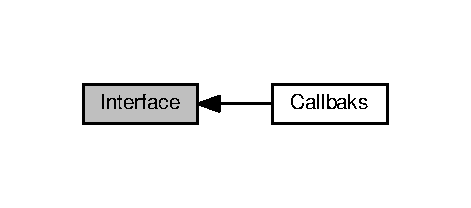
\includegraphics[width=226pt]{group__IRCInterface}
\end{center}
\end{figure}
\subsection*{Módulos}
\begin{DoxyCompactItemize}
\item 
\hyperlink{group__IRCInterfaceCallbacks}{Callbaks}
\end{DoxyCompactItemize}


\subsection{Descripción detallada}

\hypertarget{group__IRCInterfaceCallbacks}{}\section{Callbaks}
\label{group__IRCInterfaceCallbacks}\index{Callbaks@{Callbaks}}
Diagrama de colaboración para Callbaks\+:\nopagebreak
\begin{figure}[H]
\begin{center}
\leavevmode
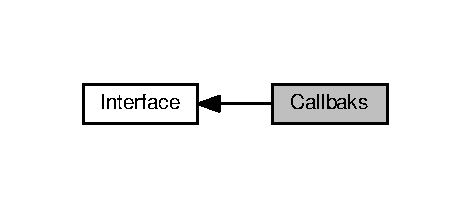
\includegraphics[width=226pt]{group__IRCInterfaceCallbacks}
\end{center}
\end{figure}
Funciones que van a ser llamadas desde el interface y que deben ser implementadas por el usuario. Todas estas funciones pertenecen al hilo del interfaz.

El programador puede, por supuesto, separar todas estas funciones en múltiples ficheros a efectos de desarrollo y modularización.



 \hypertarget{IRCInterface_ActivateChannelKey}{}\subsubsection{I\+R\+C\+Interface\+\_\+\+Activate\+Channel\+Key}\label{IRCInterface_ActivateChannelKey}
Llamada por el botón de activación de la clave del canal.


\begin{DoxyCode}
\textcolor{preprocessor}{#include <redes2/ircxchat.h>}

\textcolor{keywordtype}{void} \hyperlink{G-2313-06-P2__client_8c_a33f80a29a744e4182b29e23f13c1f05c}{IRCInterface\_ActivateChannelKey} (\textcolor{keywordtype}{char} *channel, \textcolor{keywordtype}{char} * key)
\end{DoxyCode}


Llamada por el botón de activación de la clave del canal. El segundo parámetro es la clave del canal que se desea poner. Si es N\+U\+LL deberá impedirse la activación con la función implementada a tal efecto. En cualquier caso sólo se puede realizar si el servidor acepta la orden. Las strings recibidas no deben ser manipuladas por el programador, sólo leídas.


\begin{DoxyParams}[1]{Parámetros}
\mbox{\tt in}  & {\em channel} & canal sobre el que se va a activar la clave. \\
\hline
\mbox{\tt in}  & {\em key} & clave para el canal indicado.\\
\hline
\end{DoxyParams}
\begin{DoxyWarning}{Atención}
Esta función debe ser implementada por el alumno.
\end{DoxyWarning}
\begin{DoxyAuthor}{Autor}
Eloy Anguiano (\href{mailto:eloy.anguiano@uam.es}{\tt eloy.\+anguiano@uam.\+es})
\end{DoxyAuthor}


 \hypertarget{IRCInterface_ActivateExternalMessages}{}\subsubsection{I\+R\+C\+Interface\+\_\+\+Activate\+External\+Messages}\label{IRCInterface_ActivateExternalMessages}
Llamada por el botón de activación de la recepción de mensajes externos.


\begin{DoxyCode}
\textcolor{preprocessor}{#include <redes2/ircxchat.h>}

\textcolor{keywordtype}{void} \hyperlink{G-2313-06-P2__client_8c_a7a439929c246e342ae525139b2c39f5d}{IRCInterface\_ActivateExternalMessages} (\textcolor{keywordtype}{char} *channel)
\end{DoxyCode}


Llamada por el botón de activación de la recepción de mensajes externos.

En cualquier caso sólo se puede realizar si el servidor acepta la orden. La string recibida no debe ser manipulada por el programador, sólo leída.


\begin{DoxyParams}[1]{Parámetros}
\mbox{\tt in}  & {\em channel} & canal sobre el que se activará la recepción de mensajes externos.\\
\hline
\end{DoxyParams}
\begin{DoxyWarning}{Atención}
Esta función debe ser implementada por el alumno.
\end{DoxyWarning}
\begin{DoxyAuthor}{Autor}
Eloy Anguiano (\href{mailto:eloy.anguiano@uam.es}{\tt eloy.\+anguiano@uam.\+es})
\end{DoxyAuthor}


 \hypertarget{IRCInterface_ActivateInvite}{}\subsubsection{I\+R\+C\+Interface\+\_\+\+Activate\+Invite}\label{IRCInterface_ActivateInvite}
Llamada por el botón de activación de canal de sólo invitación.


\begin{DoxyCode}
\textcolor{preprocessor}{#include <redes2/ircxchat.h>}

\textcolor{keywordtype}{void} \hyperlink{G-2313-06-P2__client_8c_ac72762ab1e3575b421b967241db23f9c}{IRCInterface\_ActivateInvite} (\textcolor{keywordtype}{char} *channel)
\end{DoxyCode}


Llamada por el botón de activación de canal de sólo invitación.

En cualquier caso sólo se puede realizar si el servidor acepta la orden. La string recibida no debe ser manipulada por el programador, sólo leída.


\begin{DoxyParams}[1]{Parámetros}
\mbox{\tt in}  & {\em channel} & canal sobre el que se activará la invitación.\\
\hline
\end{DoxyParams}
\begin{DoxyWarning}{Atención}
Esta función debe ser implementada por el alumno.
\end{DoxyWarning}
\begin{DoxyAuthor}{Autor}
Eloy Anguiano (\href{mailto:eloy.anguiano@uam.es}{\tt eloy.\+anguiano@uam.\+es})
\end{DoxyAuthor}


 \hypertarget{IRCInterface_ActivateModerated}{}\subsubsection{I\+R\+C\+Interface\+\_\+\+Activate\+Moderated}\label{IRCInterface_ActivateModerated}
Llamada por el botón de activación de la moderación del canal.


\begin{DoxyCode}
\textcolor{preprocessor}{#include <redes2/ircxchat.h>}

\textcolor{keywordtype}{void} \hyperlink{G-2313-06-P2__client_8c_af83498f4058311f4562c43a9b70566b2}{IRCInterface\_ActivateModerated} (\textcolor{keywordtype}{char} *channel)
\end{DoxyCode}


Llamada por el botón de activación de la moderación del canal.

En cualquier caso sólo se puede realizar si el servidor acepta la orden. La string recibida no debe ser manipulada por el programador, sólo leída.


\begin{DoxyParams}[1]{Parámetros}
\mbox{\tt in}  & {\em channel} & canal sobre el que se activará la moderación.\\
\hline
\end{DoxyParams}
\begin{DoxyWarning}{Atención}
Esta función debe ser implementada por el alumno.
\end{DoxyWarning}
\begin{DoxyAuthor}{Autor}
Eloy Anguiano (\href{mailto:eloy.anguiano@uam.es}{\tt eloy.\+anguiano@uam.\+es})
\end{DoxyAuthor}


 \hypertarget{IRCInterface_ActivateNicksLimit}{}\subsubsection{I\+R\+C\+Interface\+\_\+\+Activate\+Nicks\+Limit}\label{IRCInterface_ActivateNicksLimit}
Llamada por el botón de activación del límite de usuarios en el canal.


\begin{DoxyCode}
\textcolor{preprocessor}{#include <redes2/ircxchat.h>}

\textcolor{keywordtype}{void} \hyperlink{G-2313-06-P2__client_8c_ab5694cc413472173bfcaa969c7d9800e}{IRCInterface\_ActivateNicksLimit} (\textcolor{keywordtype}{char} *channel, \textcolor{keywordtype}{int} * limit)
\end{DoxyCode}


Llamada por el botón de activación del límite de usuarios en el canal. El segundo es el límite de usuarios que se desea poner. Si el valor es 0 se sobrentiende que se desea eliminar este límite.

En cualquier caso sólo se puede realizar si el servidor acepta la orden. La string recibida no debe ser manipulada por el programador, sólo leída.


\begin{DoxyParams}[1]{Parámetros}
\mbox{\tt in}  & {\em channel} & canal sobre el que se activará el límite de usuarios. \\
\hline
\mbox{\tt in}  & {\em limit} & límite de usuarios en el canal indicado.\\
\hline
\end{DoxyParams}
\begin{DoxyWarning}{Atención}
Esta función debe ser implementada por el alumno.
\end{DoxyWarning}
\begin{DoxyAuthor}{Autor}
Eloy Anguiano (\href{mailto:eloy.anguiano@uam.es}{\tt eloy.\+anguiano@uam.\+es})
\end{DoxyAuthor}


 \hypertarget{IRCInterface_ActivatePrivate}{}\subsubsection{I\+R\+C\+Interface\+\_\+\+Activate\+Private}\label{IRCInterface_ActivatePrivate}
Llamada por el botón de activación del modo privado.


\begin{DoxyCode}
\textcolor{preprocessor}{#include <redes2/ircxchat.h>}

\textcolor{keywordtype}{void} \hyperlink{G-2313-06-P2__client_8c_ab1f09c737c7c109a97e22de6072d731d}{IRCInterface\_ActivatePrivate} (\textcolor{keywordtype}{char} *channel)
\end{DoxyCode}


Llamada por el botón de activación del modo privado.

En cualquier caso sólo se puede realizar si el servidor acepta la orden. La string recibida no debe ser manipulada por el programador, sólo leída.


\begin{DoxyParams}[1]{Parámetros}
\mbox{\tt in}  & {\em channel} & canal sobre el que se va a activar la privacidad.\\
\hline
\end{DoxyParams}
\begin{DoxyWarning}{Atención}
Esta función debe ser implementada por el alumno.
\end{DoxyWarning}
\begin{DoxyAuthor}{Autor}
Eloy Anguiano (\href{mailto:eloy.anguiano@uam.es}{\tt eloy.\+anguiano@uam.\+es})
\end{DoxyAuthor}


 \hypertarget{IRCInterface_ActivateProtectTopic}{}\subsubsection{I\+R\+C\+Interface\+\_\+\+Activate\+Protect\+Topic}\label{IRCInterface_ActivateProtectTopic}
Llamada por el botón de activación de la protección de tópico.


\begin{DoxyCode}
\textcolor{preprocessor}{#include <redes2/ircxchat.h>}

\textcolor{keywordtype}{void} \hyperlink{G-2313-06-P2__client_8c_ac45f12d4dcacf3b5485eec6fdc51df93}{IRCInterface\_ActivateProtectTopic} (\textcolor{keywordtype}{char} *channel)
\end{DoxyCode}


Llamada por el botón de activación de la protección de tópico.

En cualquier caso sólo se puede realizar si el servidor acepta la orden. La string recibida no debe ser manipulada por el programador, sólo leída.


\begin{DoxyParams}[1]{Parámetros}
\mbox{\tt in}  & {\em channel} & canal sobre el que se va a activar la protección de tópico.\\
\hline
\end{DoxyParams}
\begin{DoxyWarning}{Atención}
Esta función debe ser implementada por el alumno.
\end{DoxyWarning}
\begin{DoxyAuthor}{Autor}
Eloy Anguiano (\href{mailto:eloy.anguiano@uam.es}{\tt eloy.\+anguiano@uam.\+es})
\end{DoxyAuthor}


 \hypertarget{IRCInterface_ActivateSecret}{}\subsubsection{I\+R\+C\+Interface\+\_\+\+Activate\+Secret}\label{IRCInterface_ActivateSecret}
Llamada por el botón de activación de canal secreto.


\begin{DoxyCode}
\textcolor{preprocessor}{#include <redes2/ircxchat.h>}

\textcolor{keywordtype}{void} \hyperlink{G-2313-06-P2__client_8c_aa9e9155115b834d85a4d10cb27f99093}{IRCInterface\_ActivateSecret} (\textcolor{keywordtype}{char} *channel)
\end{DoxyCode}


Llamada por el botón de activación de canal secreto.

En cualquier caso sólo se puede realizar si el servidor acepta la orden. La string recibida no debe ser manipulada por el programador, sólo leída.


\begin{DoxyParams}[1]{Parámetros}
\mbox{\tt in}  & {\em channel} & canal sobre el que se va a activar el estado de secreto.\\
\hline
\end{DoxyParams}
\begin{DoxyWarning}{Atención}
Esta función debe ser implementada por el alumno.
\end{DoxyWarning}
\begin{DoxyAuthor}{Autor}
Eloy Anguiano (\href{mailto:eloy.anguiano@uam.es}{\tt eloy.\+anguiano@uam.\+es})
\end{DoxyAuthor}


 \hypertarget{IRCInterface_BanNick}{}\subsubsection{I\+R\+C\+Interface\+\_\+\+Ban\+Nick}\label{IRCInterface_BanNick}
Llamada por el botón \char`\"{}\+Banear\char`\"{}.


\begin{DoxyCode}
\textcolor{preprocessor}{#include <redes2/ircxchat.h>}

\textcolor{keywordtype}{void} \hyperlink{G-2313-06-P2__client_8c_a42773b5a840f9d0455f148d285e1e595}{IRCInterface\_BanNick} (\textcolor{keywordtype}{char} *channel, \textcolor{keywordtype}{char} *nick)
\end{DoxyCode}


Llamada por el botón \char`\"{}\+Banear\char`\"{}. Previamente debe seleccionarse un nick del canal para darle voz a dicho usuario.

En cualquier caso sólo se puede realizar si el servidor acepta la orden. Las strings recibidas no deben ser manipuladas por el programador, sólo leídas.


\begin{DoxyParams}[1]{Parámetros}
\mbox{\tt in}  & {\em channel} & canal sobre el que se va a realizar el baneo. En principio es un valor innecesario. \\
\hline
\mbox{\tt in}  & {\em nick} & nick del usuario que va a ser baneado\\
\hline
\end{DoxyParams}
\begin{DoxyWarning}{Atención}
Esta función debe ser implementada por el alumno.
\end{DoxyWarning}
\begin{DoxyAuthor}{Autor}
Eloy Anguiano (\href{mailto:eloy.anguiano@uam.es}{\tt eloy.\+anguiano@uam.\+es})
\end{DoxyAuthor}


 \hypertarget{IRCInterface_Connect}{}\subsubsection{I\+R\+C\+Interface\+\_\+\+Connect}\label{IRCInterface_Connect}
Llamada por los distintos botones de conexión.


\begin{DoxyCode}
\textcolor{preprocessor}{#include <redes2/ircxchat.h>}

\textcolor{keywordtype}{long} \hyperlink{G-2313-06-P2__client_8c_aed072f4ce0d6e90697d4d6eb0278a2ad}{IRCInterface\_Connect} (\textcolor{keywordtype}{char} *nick, \textcolor{keywordtype}{char} * user, \textcolor{keywordtype}{char} * realname, \textcolor{keywordtype}{char} * password, \textcolor{keywordtype}{
      char} * server, \textcolor{keywordtype}{int} port, \textcolor{keywordtype}{boolean} ssl)
\end{DoxyCode}


Función a implementar por el programador. Llamada por los distintos botones de conexión. Si implementará la comunicación completa, incluido el registro del usuario en el servidor.

En cualquier caso sólo se puede realizar si el servidor acepta la orden. Las strings recibidas no deben ser manipuladas por el programador, sólo leída.


\begin{DoxyParams}[1]{Parámetros}
\mbox{\tt in}  & {\em nick} & nick con el que se va a realizar la conexíón. \\
\hline
\mbox{\tt in}  & {\em user} & usuario con el que se va a realizar la conexión. \\
\hline
\mbox{\tt in}  & {\em realname} & nombre real con el que se va a realizar la conexión. \\
\hline
\mbox{\tt in}  & {\em password} & password del usuario si es necesaria, puede valer N\+U\+LL. \\
\hline
\mbox{\tt in}  & {\em server} & nombre o ip del servidor con el que se va a realizar la conexión. \\
\hline
\mbox{\tt in}  & {\em port} & puerto del servidor con el que se va a realizar la conexión. \\
\hline
\mbox{\tt in}  & {\em ssl} & puede ser T\+R\+UE si la conexión tiene que ser segura y F\+A\+L\+SE si no es así.\\
\hline
\end{DoxyParams}

\begin{DoxyRetVals}{Valores devueltos}
{\em I\+R\+C\+\_\+\+OK} & si todo ha sido correcto (debe devolverlo). \\
\hline
{\em I\+R\+C\+E\+R\+R\+\_\+\+N\+O\+S\+SL} & si el valor de S\+SL es T\+R\+UE y no se puede activar la conexión S\+SL pero sí una conexión no protegida (debe devolverlo). \\
\hline
{\em I\+R\+C\+E\+R\+R\+\_\+\+N\+O\+C\+O\+N\+N\+E\+CT} & en caso de que no se pueda realizar la comunicación (debe devolverlo).\\
\hline
\end{DoxyRetVals}
\begin{DoxyWarning}{Atención}
Esta función debe ser implementada por el alumno.
\end{DoxyWarning}
\begin{DoxyAuthor}{Autor}
Eloy Anguiano (\href{mailto:eloy.anguiano@uam.es}{\tt eloy.\+anguiano@uam.\+es})
\end{DoxyAuthor}


 \hypertarget{IRCInterface_DeactivateChannelKey}{}\subsubsection{I\+R\+C\+Interface\+\_\+\+Deactivate\+Channel\+Key}\label{IRCInterface_DeactivateChannelKey}
Llamada por el botón de desactivación de la clave del canal.


\begin{DoxyCode}
\textcolor{preprocessor}{#include <redes2/ircxchat.h>}

\textcolor{keywordtype}{void} \hyperlink{G-2313-06-P2__client_8c_a3e67ee0cd384b524d57fda14593dce8e}{IRCInterface\_DeactivateChannelKey} (\textcolor{keywordtype}{char} *channel)
\end{DoxyCode}


Llamada por el botón de desactivación de la clave del canal.

En cualquier caso sólo se puede realizar si el servidor acepta la orden. La string recibida no debe ser manipulada por el programador, sólo leída.


\begin{DoxyParams}[1]{Parámetros}
\mbox{\tt in}  & {\em channel} & canal sobre el que se va a desactivar la clave.\\
\hline
\end{DoxyParams}
\begin{DoxyWarning}{Atención}
Esta función debe ser implementada por el alumno.
\end{DoxyWarning}
\begin{DoxyAuthor}{Autor}
Eloy Anguiano (\href{mailto:eloy.anguiano@uam.es}{\tt eloy.\+anguiano@uam.\+es})
\end{DoxyAuthor}


 \hypertarget{IRCInterface_DeactivateExternalMessages}{}\subsubsection{I\+R\+C\+Interface\+\_\+\+Deactivate\+External\+Messages}\label{IRCInterface_DeactivateExternalMessages}
Llamada por el botón de desactivación de la recepción de mensajes externos.


\begin{DoxyCode}
\textcolor{preprocessor}{#include <redes2/ircxchat.h>}

\textcolor{keywordtype}{void} \hyperlink{G-2313-06-P2__client_8c_a638b1535f4ecbc9a6affb2df2a6a946e}{IRCInterface\_DeactivateExternalMessages} (\textcolor{keywordtype}{char} *channel)
\end{DoxyCode}


Llamada por el botón de desactivación de la recepción de mensajes externos.

En cualquier caso sólo se puede realizar si el servidor acepta la orden. La string recibida no debe ser manipulada por el programador, sólo leída.


\begin{DoxyParams}[1]{Parámetros}
\mbox{\tt in}  & {\em channel} & canal sobre el que se va a deactivar la recepción de mensajes externos.\\
\hline
\end{DoxyParams}
\begin{DoxyWarning}{Atención}
Esta función debe ser implementada por el alumno.
\end{DoxyWarning}
\begin{DoxyAuthor}{Autor}
Eloy Anguiano (\href{mailto:eloy.anguiano@uam.es}{\tt eloy.\+anguiano@uam.\+es})
\end{DoxyAuthor}


 \hypertarget{IRCInterface_DeactivateInvite}{}\subsubsection{I\+R\+C\+Interface\+\_\+\+Deactivate\+Invite}\label{IRCInterface_DeactivateInvite}
Llamada por el botón de desactivación de canal de sólo invitación.


\begin{DoxyCode}
\textcolor{preprocessor}{#include <redes2/ircxchat.h>}

\textcolor{keywordtype}{void} \hyperlink{G-2313-06-P2__client_8c_a9ba4e98a3729737aa63ebec54ba4e894}{IRCInterface\_DeactivateInvite} (\textcolor{keywordtype}{char} *channel)
\end{DoxyCode}


Llamada por el botón de desactivación de canal de sólo invitación.

En cualquier caso sólo se puede realizar si el servidor acepta la orden. La string recibida no debe ser manipulada por el programador, sólo leída.


\begin{DoxyParams}[1]{Parámetros}
\mbox{\tt in}  & {\em channel} & canal sobre el que se va a desactivar la invitación.\\
\hline
\end{DoxyParams}
\begin{DoxyWarning}{Atención}
Esta función debe ser implementada por el alumno.
\end{DoxyWarning}
\begin{DoxyAuthor}{Autor}
Eloy Anguiano (\href{mailto:eloy.anguiano@uam.es}{\tt eloy.\+anguiano@uam.\+es})
\end{DoxyAuthor}


 \hypertarget{IRCInterface_DeactivateModerated}{}\subsubsection{I\+R\+C\+Interface\+\_\+\+Deactivate\+Moderated}\label{IRCInterface_DeactivateModerated}
Llamada por el botón de desactivación de la moderación del canal.


\begin{DoxyCode}
\textcolor{preprocessor}{#include <redes2/ircxchat.h>}

\textcolor{keywordtype}{void} \hyperlink{G-2313-06-P2__client_8c_ab760e8144b38f6c14bd809d157cee5d4}{IRCInterface\_DeactivateModerated} (\textcolor{keywordtype}{char} *channel)
\end{DoxyCode}


Llamada por el botón de desactivación de la moderación del canal.

En cualquier caso sólo se puede realizar si el servidor acepta la orden. La string recibida no debe ser manipulada por el programador, sólo leída.


\begin{DoxyParams}[1]{Parámetros}
\mbox{\tt in}  & {\em channel} & canal sobre el que se va a desactivar la moderación.\\
\hline
\end{DoxyParams}
\begin{DoxyWarning}{Atención}
Esta función debe ser implementada por el alumno.
\end{DoxyWarning}
\begin{DoxyAuthor}{Autor}
Eloy Anguiano (\href{mailto:eloy.anguiano@uam.es}{\tt eloy.\+anguiano@uam.\+es})
\end{DoxyAuthor}


 \hypertarget{IRCInterface_DeactivateNicksLimit}{}\subsubsection{I\+R\+C\+Interface\+\_\+\+Deactivate\+Nicks\+Limit}\label{IRCInterface_DeactivateNicksLimit}
Llamada por el botón de desactivación de la protección de tópico.


\begin{DoxyCode}
\textcolor{preprocessor}{#include <redes2/ircxchat.h>}

\textcolor{keywordtype}{void} \hyperlink{G-2313-06-P2__client_8c_a92c8cfbe2e14e19277e1c97d11719e80}{IRCInterface\_DeactivateNicksLimit} (\textcolor{keywordtype}{char} *channel)
\end{DoxyCode}


Llamada por el botón de desactivación del límite de usuarios en el canal.

En cualquier caso sólo se puede realizar si el servidor acepta la orden. La string recibida no debe ser manipulada por el programador, sólo leída.


\begin{DoxyParams}[1]{Parámetros}
\mbox{\tt in}  & {\em channel} & canal sobre el que se va a desactivar el límite de usuarios.\\
\hline
\end{DoxyParams}
\begin{DoxyWarning}{Atención}
Esta función debe ser implementada por el alumno.
\end{DoxyWarning}
\begin{DoxyAuthor}{Autor}
Eloy Anguiano (\href{mailto:eloy.anguiano@uam.es}{\tt eloy.\+anguiano@uam.\+es})
\end{DoxyAuthor}


 \hypertarget{IRCInterface_DeactivatePrivate}{}\subsubsection{I\+R\+C\+Interface\+\_\+\+Deactivate\+Private}\label{IRCInterface_DeactivatePrivate}
Llamada por el botón de desactivación del modo privado.


\begin{DoxyCode}
\textcolor{preprocessor}{#include <redes2/ircxchat.h>}

\textcolor{keywordtype}{void} \hyperlink{G-2313-06-P2__client_8c_a8a6141803691ba327f11ba763ad075d4}{IRCInterface\_DeactivatePrivate} (\textcolor{keywordtype}{char} *channel)
\end{DoxyCode}


Llamada por el botón de desactivación del modo privado.

En cualquier caso sólo se puede realizar si el servidor acepta la orden. La string recibida no debe ser manipulada por el programador, sólo leída.

\begin{DoxyWarning}{Atención}
Esta función debe ser implementada por el alumno.
\end{DoxyWarning}

\begin{DoxyParams}[1]{Parámetros}
\mbox{\tt in}  & {\em channel} & canal sobre el que se va a desactivar la privacidad.\\
\hline
\end{DoxyParams}
\begin{DoxyWarning}{Atención}
Esta función debe ser implementada por el alumno.
\end{DoxyWarning}
\begin{DoxyAuthor}{Autor}
Eloy Anguiano (\href{mailto:eloy.anguiano@uam.es}{\tt eloy.\+anguiano@uam.\+es})
\end{DoxyAuthor}


 \hypertarget{IRCInterface_DeactivateProtectTopic}{}\subsubsection{I\+R\+C\+Interface\+\_\+\+Deactivate\+Protect\+Topic}\label{IRCInterface_DeactivateProtectTopic}
Llamada por el botón de desactivación de la protección de tópico.


\begin{DoxyCode}
\textcolor{preprocessor}{#include <redes2/ircxchat.h>}

\textcolor{keywordtype}{void} \hyperlink{G-2313-06-P2__client_8c_a5a57541a950f8c2c40b4b44c32b28ed9}{IRCInterface\_DeactivateProtectTopic} (\textcolor{keywordtype}{char} *channel)
\end{DoxyCode}


Llamada por el botón de desactivación de la protección de tópico.

En cualquier caso sólo se puede realizar si el servidor acepta la orden. La string recibida no debe ser manipulada por el programador, sólo leída.


\begin{DoxyParams}[1]{Parámetros}
\mbox{\tt in}  & {\em channel} & canal sobre el que se va a desactivar la protección de tópico.\\
\hline
\end{DoxyParams}
\begin{DoxyWarning}{Atención}
Esta función debe ser implementada por el alumno.
\end{DoxyWarning}
\begin{DoxyAuthor}{Autor}
Eloy Anguiano (\href{mailto:eloy.anguiano@uam.es}{\tt eloy.\+anguiano@uam.\+es})
\end{DoxyAuthor}


 \hypertarget{IRCInterface_DeactivateSecret}{}\subsubsection{I\+R\+C\+Interface\+\_\+\+Deactivate\+Secret}\label{IRCInterface_DeactivateSecret}
Llamada por el botón de desactivación de canal secreto.


\begin{DoxyCode}
\textcolor{preprocessor}{#include <redes2/ircxchat.h>}

\textcolor{keywordtype}{void} \hyperlink{G-2313-06-P2__client_8c_a4956427664cabc7d5b2bd1589a207324}{IRCInterface\_DeactivateSecret} (\textcolor{keywordtype}{char} *channel)
\end{DoxyCode}


Llamada por el botón de desactivación de canal secreto.

En cualquier caso sólo se puede realizar si el servidor acepta la orden. La string recibida no debe ser manipulada por el programador, sólo leída.


\begin{DoxyParams}[1]{Parámetros}
\mbox{\tt in}  & {\em channel} & canal sobre el que se va a desactivar la propiedad de canal secreto.\\
\hline
\end{DoxyParams}
\begin{DoxyWarning}{Atención}
Esta función debe ser implementada por el alumno.
\end{DoxyWarning}
\begin{DoxyAuthor}{Autor}
Eloy Anguiano (\href{mailto:eloy.anguiano@uam.es}{\tt eloy.\+anguiano@uam.\+es})
\end{DoxyAuthor}


 \hypertarget{IRCInterface_DisconnectServer}{}\subsubsection{I\+R\+C\+Interface\+\_\+\+Disconnect\+Server}\label{IRCInterface_DisconnectServer}
Llamada por los distintos botones de desconexión.


\begin{DoxyCode}
\textcolor{preprocessor}{#include <redes2/ircxchat.h>}

\textcolor{keywordtype}{boolean} \hyperlink{G-2313-06-P2__client_8c_a8bf0424ef7f845be79a056e9aed56fe2}{IRCInterface\_DisconnectServer} (\textcolor{keywordtype}{char} * server, \textcolor{keywordtype}{int} port)
\end{DoxyCode}


Llamada por los distintos botones de desconexión. Debe cerrar la conexión con el servidor.

En cualquier caso sólo se puede realizar si el servidor acepta la orden. La string recibida no debe ser manipulada por el programador, sólo leída.


\begin{DoxyParams}[1]{Parámetros}
\mbox{\tt in}  & {\em server} & nombre o ip del servidor del que se va a realizar la desconexión. \\
\hline
\mbox{\tt in}  & {\em port} & puerto sobre el que se va a realizar la desconexión.\\
\hline
\end{DoxyParams}

\begin{DoxyRetVals}{Valores devueltos}
{\em T\+R\+UE} & si se ha cerrado la conexión (debe devolverlo). \\
\hline
{\em F\+A\+L\+SE} & en caso contrario (debe devolverlo).\\
\hline
\end{DoxyRetVals}
\begin{DoxyWarning}{Atención}
Esta función debe ser implementada por el alumno.
\end{DoxyWarning}
\begin{DoxyAuthor}{Autor}
Eloy Anguiano (\href{mailto:eloy.anguiano@uam.es}{\tt eloy.\+anguiano@uam.\+es})
\end{DoxyAuthor}


 \hypertarget{IRCInterface_ExitAudioChat}{}\subsubsection{I\+R\+C\+Interface\+\_\+\+Exit\+Audio\+Chat}\label{IRCInterface_ExitAudioChat}
Llamada por el botón \char`\"{}\+Cancelar\char`\"{} del diálogo de chat de voz.


\begin{DoxyCode}
\textcolor{preprocessor}{#include <redes2/ircxchat.h>}

\textcolor{keywordtype}{void} \hyperlink{G-2313-06-P2__client_8c_ab431412191716f751461f94d613ffdab}{IRCInterface\_ExitAudioChat} (\textcolor{keywordtype}{char} *nick)
\end{DoxyCode}


Llamada por el botón \char`\"{}\+Parar\char`\"{} del diálogo de chat de voz. Previamente debe seleccionarse un nick del canal para darle voz a dicho usuario. Esta función cierrala comunicación. Evidentemente tiene que actuar sobre el hilo de chat de voz.

En cualquier caso sólo se puede realizar si el servidor acepta la orden. La string recibida no debe ser manipulada por el programador, sólo leída.


\begin{DoxyParams}[1]{Parámetros}
\mbox{\tt in}  & {\em nick} & nick del usuario que solicita la parada del chat de audio.\\
\hline
\end{DoxyParams}

\begin{DoxyRetVals}{Valores devueltos}
{\em T\+R\+UE} & si se ha cerrado la comunicación (debe devolverlo). \\
\hline
{\em F\+A\+L\+SE} & en caso contrario (debe devolverlo).\\
\hline
\end{DoxyRetVals}
\begin{DoxyWarning}{Atención}
Esta función debe ser implementada por el alumno.
\end{DoxyWarning}
\begin{DoxyAuthor}{Autor}
Eloy Anguiano (\href{mailto:eloy.anguiano@uam.es}{\tt eloy.\+anguiano@uam.\+es})
\end{DoxyAuthor}


 \hypertarget{IRCInterface_GiveOp}{}\subsubsection{I\+R\+C\+Interface\+\_\+\+Give\+Op}\label{IRCInterface_GiveOp}
Llamada por el botón \char`\"{}\+Op\char`\"{}.


\begin{DoxyCode}
\textcolor{preprocessor}{#include <redes2/ircxchat.h>}

\textcolor{keywordtype}{void} \hyperlink{G-2313-06-P2__client_8c_ae075029bb55e8b995f22beb0810674f4}{IRCInterface\_GiveOp} (\textcolor{keywordtype}{char} *channel, \textcolor{keywordtype}{char} *nick)
\end{DoxyCode}


Llamada por el botón \char`\"{}\+Op\char`\"{}. Previamente debe seleccionarse un nick del canal para darle \char`\"{}op\char`\"{} a dicho usuario.

En cualquier caso sólo se puede realizar si el servidor acepta la orden. Las strings recibidas no deben ser manipuladas por el programador, sólo leídas.


\begin{DoxyParams}[1]{Parámetros}
\mbox{\tt in}  & {\em channel} & canal sobre el que se va dar op al usuario. \\
\hline
\mbox{\tt in}  & {\em nick} & nick al que se le va a dar el nivel de op.\\
\hline
\end{DoxyParams}
\begin{DoxyWarning}{Atención}
Esta función debe ser implementada por el alumno.
\end{DoxyWarning}
\begin{DoxyAuthor}{Autor}
Eloy Anguiano (\href{mailto:eloy.anguiano@uam.es}{\tt eloy.\+anguiano@uam.\+es})
\end{DoxyAuthor}


 \hypertarget{IRCInterface_GiveVoice}{}\subsubsection{I\+R\+C\+Interface\+\_\+\+Give\+Voice}\label{IRCInterface_GiveVoice}
Llamada por el botón \char`\"{}\+Dar voz\char`\"{}.


\begin{DoxyCode}
\textcolor{preprocessor}{#include <redes2/ircxchat.h>}

\textcolor{keywordtype}{void} \hyperlink{G-2313-06-P2__client_8c_ae9effb4bdaf4a2cdf2dd9edbeb90b430}{IRCInterface\_GiveVoice} (\textcolor{keywordtype}{char} *channel, \textcolor{keywordtype}{char} *nick)
\end{DoxyCode}


Llamada por el botón \char`\"{}\+Dar voz\char`\"{}. Previamente debe seleccionarse un nick del canal para darle voz a dicho usuario.

En cualquier caso sólo se puede realizar si el servidor acepta la orden. Las strings recibidas no deben ser manipuladas por el programador, sólo leídas.


\begin{DoxyParams}[1]{Parámetros}
\mbox{\tt in}  & {\em channel} & canal sobre el que se va dar voz al usuario. \\
\hline
\mbox{\tt in}  & {\em nick} & nick al que se le va a dar voz.\\
\hline
\end{DoxyParams}
\begin{DoxyWarning}{Atención}
Esta función debe ser implementada por el alumno.
\end{DoxyWarning}
\begin{DoxyAuthor}{Autor}
Eloy Anguiano (\href{mailto:eloy.anguiano@uam.es}{\tt eloy.\+anguiano@uam.\+es})
\end{DoxyAuthor}


 \hypertarget{IRCInterface_KickNick}{}\subsubsection{I\+R\+C\+Interface\+\_\+\+Kick\+Nick}\label{IRCInterface_KickNick}
Llamada por el botón \char`\"{}\+Echar\char`\"{}.


\begin{DoxyCode}
\textcolor{preprocessor}{#include <redes2/ircxchat.h>}

\textcolor{keywordtype}{void} \hyperlink{G-2313-06-P2__client_8c_a7adfea400a96160585f86179bafb055f}{IRCInterface\_KickNick} (\textcolor{keywordtype}{char} *channel, \textcolor{keywordtype}{char} *nick)
\end{DoxyCode}


Llamada por el botón \char`\"{}\+Echar\char`\"{}. Previamente debe seleccionarse un nick del canal para darle voz a dicho usuario.

En cualquier caso sólo se puede realizar si el servidor acepta la orden. Las strings recibidas no deben ser manipuladas por el programador, sólo leídas.


\begin{DoxyParams}[1]{Parámetros}
\mbox{\tt in}  & {\em channel} & canal sobre el que se va a expulsar al usuario. \\
\hline
\mbox{\tt in}  & {\em nick} & nick del usuario que va a ser expulsado.\\
\hline
\end{DoxyParams}
\begin{DoxyWarning}{Atención}
Esta función debe ser implementada por el alumno.
\end{DoxyWarning}
\begin{DoxyAuthor}{Autor}
Eloy Anguiano (\href{mailto:eloy.anguiano@uam.es}{\tt eloy.\+anguiano@uam.\+es})
\end{DoxyAuthor}


 \hypertarget{IRCInterface_NewCommandText}{}\subsubsection{I\+R\+C\+Interface\+\_\+\+New\+Command\+Text}\label{IRCInterface_NewCommandText}
Llamada la tecla E\+N\+T\+ER en el campo de texto y comandos.


\begin{DoxyCode}
\textcolor{preprocessor}{#include <redes2/ircxchat.h>}

\textcolor{keywordtype}{void} \hyperlink{G-2313-06-P2__client_8c_a214e10b19c8be028fb35d2a7abf3f798}{IRCInterface\_NewCommandText} (\textcolor{keywordtype}{char} *command)
\end{DoxyCode}


Llamada de la tecla E\+N\+T\+ER en el campo de texto y comandos. El texto deberá ser enviado y el comando procesado por las funciones de \char`\"{}parseo\char`\"{} de comandos de usuario.

En cualquier caso sólo se puede realizar si el servidor acepta la orden. La string recibida no debe ser manipulada por el programador, sólo leída.


\begin{DoxyParams}[1]{Parámetros}
\mbox{\tt in}  & {\em comando} & introducido por el usuario.\\
\hline
\end{DoxyParams}
\begin{DoxyWarning}{Atención}
Esta función debe ser implementada por el alumno.
\end{DoxyWarning}
\begin{DoxyAuthor}{Autor}
Eloy Anguiano (\href{mailto:eloy.anguiano@uam.es}{\tt eloy.\+anguiano@uam.\+es})
\end{DoxyAuthor}


 \hypertarget{IRCInterface_NewTopicEnter}{}\subsubsection{I\+R\+C\+Interface\+\_\+\+New\+Topic\+Enter}\label{IRCInterface_NewTopicEnter}
Llamada cuando se pulsa la tecla E\+N\+T\+ER en el campo de tópico.


\begin{DoxyCode}
\textcolor{preprocessor}{#include <redes2/ircxchat.h>}

\textcolor{keywordtype}{void} \hyperlink{G-2313-06-P2__client_8c_a080cf34ff506481737f6d08af60ca92b}{IRCInterface\_NewTopicEnter} (\textcolor{keywordtype}{char} * topicdata)
\end{DoxyCode}


Llamada cuando se pulsa la tecla E\+N\+T\+ER en el campo de tópico. Deberá intentarse cambiar el tópico del canal.

En cualquier caso sólo se puede realizar si el servidor acepta la orden. La string recibida no debe ser manipulada por el programador, sólo leída.

param\mbox{[}in\mbox{]} topicdata string con el tópico que se desea poner en el canal.

\begin{DoxyWarning}{Atención}
Esta función debe ser implementada por el alumno.
\end{DoxyWarning}
\begin{DoxyAuthor}{Autor}
Eloy Anguiano (\href{mailto:eloy.anguiano@uam.es}{\tt eloy.\+anguiano@uam.\+es})
\end{DoxyAuthor}


 \hypertarget{IRCInterface_SendFile}{}\subsubsection{I\+R\+C\+Interface\+\_\+\+Send\+File}\label{IRCInterface_SendFile}
Llamada por el botón \char`\"{}\+Enviar Archivo\char`\"{}.


\begin{DoxyCode}
\textcolor{preprocessor}{#include <redes2/ircxchat.h>}

\textcolor{keywordtype}{void} \hyperlink{G-2313-06-P2__client_8c_a100f1c87bb3b399a7284e62dd2e6172a}{IRCInterface\_SendFile} (\textcolor{keywordtype}{char} * filename, \textcolor{keywordtype}{char} *nick, \textcolor{keywordtype}{char} *data, \textcolor{keywordtype}{long} \textcolor{keywordtype}{unsigned} \textcolor{keywordtype}{int}
       length)
\end{DoxyCode}


Llamada por el botón \char`\"{}\+Enviar Archivo\char`\"{}. Previamente debe seleccionarse un nick del canal para darle voz a dicho usuario. Esta función como todos los demás callbacks bloquea el interface y por tanto es el programador el que debe determinar si crea un nuevo hilo para enviar el archivo o no lo hace.

En cualquier caso sólo se puede realizar si el servidor acepta la orden. Las strings recibidas no deben ser manipuladas por el programador, sólo leídas.


\begin{DoxyParams}[1]{Parámetros}
\mbox{\tt in}  & {\em filename} & nombre del fichero a enviar. \\
\hline
\mbox{\tt in}  & {\em nick} & nick del usuario que enviará el fichero. \\
\hline
\mbox{\tt in}  & {\em data} & datos a ser enviados. \\
\hline
\mbox{\tt in}  & {\em length} & longitud de los datos a ser enviados.\\
\hline
\end{DoxyParams}

\begin{DoxyRetVals}{Valores devueltos}
{\em T\+R\+UE} & si se ha establecido la comunicación (debe devolverlo). \\
\hline
{\em F\+A\+L\+SE} & en caso contrario (debe devolverlo).\\
\hline
\end{DoxyRetVals}
\begin{DoxyWarning}{Atención}
Esta función debe ser implementada por el alumno.
\end{DoxyWarning}
\begin{DoxyAuthor}{Autor}
Eloy Anguiano (\href{mailto:eloy.anguiano@uam.es}{\tt eloy.\+anguiano@uam.\+es})
\end{DoxyAuthor}


 \hypertarget{IRCInterface_StartAudioChat}{}\subsubsection{I\+R\+C\+Interface\+\_\+\+Start\+Audio\+Chat}\label{IRCInterface_StartAudioChat}
Llamada por el botón \char`\"{}\+Iniciar\char`\"{} del diálogo de chat de voz.


\begin{DoxyCode}
\textcolor{preprocessor}{#include <redes2/ircxchat.h>}

\textcolor{keywordtype}{void} \hyperlink{G-2313-06-P2__client_8c_a5dc7a44587e609b416a783cd420a12e3}{IRCInterface\_StartAudioChat} (\textcolor{keywordtype}{char} *nick)
\end{DoxyCode}


Llamada por el botón \char`\"{}\+Iniciar\char`\"{} del diálogo de chat de voz. Previamente debe seleccionarse un nick del canal para darle voz a dicho usuario. Esta función como todos los demás callbacks bloquea el interface y por tanto para mantener la funcionalidad del chat de voz es imprescindible crear un hilo a efectos de comunicación de voz.

En cualquier caso sólo se puede realizar si el servidor acepta la orden. La string recibida no debe ser manipulada por el programador, sólo leída.


\begin{DoxyParams}[1]{Parámetros}
\mbox{\tt in}  & {\em nick} & nick del usuario con el que se desea conectar.\\
\hline
\end{DoxyParams}

\begin{DoxyRetVals}{Valores devueltos}
{\em T\+R\+UE} & si se ha establecido la comunicación (debe devolverlo). \\
\hline
{\em F\+A\+L\+SE} & en caso contrario (debe devolverlo).\\
\hline
\end{DoxyRetVals}
\begin{DoxyWarning}{Atención}
Esta función debe ser implementada por el alumno.
\end{DoxyWarning}
\begin{DoxyAuthor}{Autor}
Eloy Anguiano (\href{mailto:eloy.anguiano@uam.es}{\tt eloy.\+anguiano@uam.\+es})
\end{DoxyAuthor}


 \hypertarget{IRCInterface_StopAudioChat}{}\subsubsection{I\+R\+C\+Interface\+\_\+\+Stop\+Audio\+Chat}\label{IRCInterface_StopAudioChat}
Llamada por el botón \char`\"{}\+Parar\char`\"{} del diálogo de chat de voz.


\begin{DoxyCode}
\textcolor{preprocessor}{#include <redes2/ircxchat.h>}

\textcolor{keywordtype}{void} \hyperlink{G-2313-06-P2__client_8c_a754a3d3dd311194637c07cc701e7d507}{IRCInterface\_StopAudioChat} (\textcolor{keywordtype}{char} *nick)
\end{DoxyCode}


Llamada por el botón \char`\"{}\+Parar\char`\"{} del diálogo de chat de voz. Previamente debe seleccionarse un nick del canal para darle voz a dicho usuario. Esta función sólo para la comunicación que puede ser reiniciada. Evidentemente tiene que actuar sobre el hilo de chat de voz.

En cualquier caso sólo se puede realizar si el servidor acepta la orden. La string recibida no debe ser manipulada por el programador, sólo leída.


\begin{DoxyParams}[1]{Parámetros}
\mbox{\tt in}  & {\em nick} & nick del usuario con el que se quiere parar el chat de voz.\\
\hline
\end{DoxyParams}

\begin{DoxyRetVals}{Valores devueltos}
{\em T\+R\+UE} & si se ha parado la comunicación (debe devolverlo). \\
\hline
{\em F\+A\+L\+SE} & en caso contrario (debe devolverlo).\\
\hline
\end{DoxyRetVals}
\begin{DoxyWarning}{Atención}
Esta función debe ser implementada por el alumno.
\end{DoxyWarning}
\begin{DoxyAuthor}{Autor}
Eloy Anguiano (\href{mailto:eloy.anguiano@uam.es}{\tt eloy.\+anguiano@uam.\+es})
\end{DoxyAuthor}


 \hypertarget{IRCInterface_TakeOp}{}\subsubsection{I\+R\+C\+Interface\+\_\+\+Take\+Op}\label{IRCInterface_TakeOp}
Llamada por el botón \char`\"{}\+Quitar Op\char`\"{}.


\begin{DoxyCode}
\textcolor{preprocessor}{#include <redes2/ircxchat.h>}

\textcolor{keywordtype}{void} \hyperlink{G-2313-06-P2__client_8c_a4e2a1ea75e59306142030a91a054b7e6}{IRCInterface\_TakeOp} (\textcolor{keywordtype}{char} *channel, \textcolor{keywordtype}{char} *nick)
\end{DoxyCode}


Llamada por el botón \char`\"{}\+Quitar Op\char`\"{}. Previamente debe seleccionarse un nick del canal para quitarle \char`\"{}op\char`\"{} a dicho usuario.

En cualquier caso sólo se puede realizar si el servidor acepta la orden. Las strings recibidas no deben ser manipuladas por el programador, sólo leídas.


\begin{DoxyParams}[1]{Parámetros}
\mbox{\tt in}  & {\em channel} & canal sobre el que se va a quitar op al usuario. \\
\hline
\mbox{\tt in}  & {\em nick} & nick del usuario al que se le va a quitar op.\\
\hline
\end{DoxyParams}
\begin{DoxyWarning}{Atención}
Esta función debe ser implementada por el alumno.
\end{DoxyWarning}
\begin{DoxyAuthor}{Autor}
Eloy Anguiano (\href{mailto:eloy.anguiano@uam.es}{\tt eloy.\+anguiano@uam.\+es})
\end{DoxyAuthor}


 \hypertarget{IRCInterface_TakeVoice}{}\subsubsection{I\+R\+C\+Interface\+\_\+\+Take\+Voice}\label{IRCInterface_TakeVoice}
Llamada por el botón \char`\"{}\+Quitar voz\char`\"{}.


\begin{DoxyCode}
\textcolor{preprocessor}{#include <redes2/ircxchat.h>}

\textcolor{keywordtype}{void} \hyperlink{G-2313-06-P2__client_8c_a2ff2e10ed1cb1a399293b6f76ac1e5ae}{IRCInterface\_TakeVoice} (\textcolor{keywordtype}{char} *channel, \textcolor{keywordtype}{char} *nick)
\end{DoxyCode}


Llamada por el botón \char`\"{}\+Quitar voz\char`\"{}. Previamente debe seleccionarse un nick del canal para darle voz a dicho usuario.

En cualquier caso sólo se puede realizar si el servidor acepta la orden. Las strings recibidas no deben ser manipuladas por el programador, sólo leídas.


\begin{DoxyParams}[1]{Parámetros}
\mbox{\tt in}  & {\em channel} & canal sobre el que se le va a quitar voz al usuario. \\
\hline
\mbox{\tt in}  & {\em nick} & nick del usuario al que se va a quitar la voz.\\
\hline
\end{DoxyParams}
\begin{DoxyWarning}{Atención}
Esta función debe ser implementada por el alumno.
\end{DoxyWarning}
\begin{DoxyAuthor}{Autor}
Eloy Anguiano (\href{mailto:eloy.anguiano@uam.es}{\tt eloy.\+anguiano@uam.\+es})
\end{DoxyAuthor}


 
\chapter{Documentación de las clases}
\hypertarget{structsrecv}{}\section{Referencia de la Estructura srecv}
\label{structsrecv}\index{srecv@{srecv}}


{\ttfamily \#include $<$G-\/2313-\/06-\/\+P2\+\_\+files.\+h$>$}

\subsection*{Atributos públicos}
\begin{DoxyCompactItemize}
\item 
char $\ast$ \hyperlink{structsrecv_abe3a30e845f4f2f6e47aac6583af3166}{nick}
\item 
char $\ast$ \hyperlink{structsrecv_a6ec350741c1d09ab84e115dfde89aa82}{filename}
\item 
char $\ast$ \hyperlink{structsrecv_ac5ef113d83ca6646b0cc58b757e22f78}{data}
\item 
long unsigned \hyperlink{structsrecv_af681620ef61aa562c7d575773f156761}{length}
\end{DoxyCompactItemize}


\subsection{Descripción detallada}


Definición en la línea 29 del archivo G-\/2313-\/06-\/\+P2\+\_\+files.\+h.



\subsection{Documentación de los datos miembro}
\index{srecv@{srecv}!data@{data}}
\index{data@{data}!srecv@{srecv}}
\subsubsection[{\texorpdfstring{data}{data}}]{\setlength{\rightskip}{0pt plus 5cm}char$\ast$ srecv\+::data}\hypertarget{structsrecv_ac5ef113d83ca6646b0cc58b757e22f78}{}\label{structsrecv_ac5ef113d83ca6646b0cc58b757e22f78}


Definición en la línea 32 del archivo G-\/2313-\/06-\/\+P2\+\_\+files.\+h.

\index{srecv@{srecv}!filename@{filename}}
\index{filename@{filename}!srecv@{srecv}}
\subsubsection[{\texorpdfstring{filename}{filename}}]{\setlength{\rightskip}{0pt plus 5cm}char$\ast$ srecv\+::filename}\hypertarget{structsrecv_a6ec350741c1d09ab84e115dfde89aa82}{}\label{structsrecv_a6ec350741c1d09ab84e115dfde89aa82}


Definición en la línea 31 del archivo G-\/2313-\/06-\/\+P2\+\_\+files.\+h.

\index{srecv@{srecv}!length@{length}}
\index{length@{length}!srecv@{srecv}}
\subsubsection[{\texorpdfstring{length}{length}}]{\setlength{\rightskip}{0pt plus 5cm}long unsigned srecv\+::length}\hypertarget{structsrecv_af681620ef61aa562c7d575773f156761}{}\label{structsrecv_af681620ef61aa562c7d575773f156761}


Definición en la línea 33 del archivo G-\/2313-\/06-\/\+P2\+\_\+files.\+h.

\index{srecv@{srecv}!nick@{nick}}
\index{nick@{nick}!srecv@{srecv}}
\subsubsection[{\texorpdfstring{nick}{nick}}]{\setlength{\rightskip}{0pt plus 5cm}char$\ast$ srecv\+::nick}\hypertarget{structsrecv_abe3a30e845f4f2f6e47aac6583af3166}{}\label{structsrecv_abe3a30e845f4f2f6e47aac6583af3166}


Definición en la línea 30 del archivo G-\/2313-\/06-\/\+P2\+\_\+files.\+h.



La documentación para esta estructura fue generada a partir del siguiente fichero\+:\begin{DoxyCompactItemize}
\item 
includes/\hyperlink{G-2313-06-P2__files_8h}{G-\/2313-\/06-\/\+P2\+\_\+files.\+h}\end{DoxyCompactItemize}

\chapter{Documentación de archivos}
\hypertarget{G-2313-06-P2__client_8h}{}\section{Referencia del Archivo includes/\+G-\/2313-\/06-\/\+P2\+\_\+client.h}
\label{G-2313-06-P2__client_8h}\index{includes/\+G-\/2313-\/06-\/\+P2\+\_\+client.\+h@{includes/\+G-\/2313-\/06-\/\+P2\+\_\+client.\+h}}
{\ttfamily \#include $<$errno.\+h$>$}\\*
{\ttfamily \#include $<$sys/time.\+h$>$}\\*
{\ttfamily \#include $<$unistd.\+h$>$}\\*
{\ttfamily \#include $<$sys/types.\+h$>$}\\*
{\ttfamily \#include $<$sys/socket.\+h$>$}\\*
{\ttfamily \#include $<$sys/stat.\+h$>$}\\*
{\ttfamily \#include $<$netinet/in.\+h$>$}\\*
{\ttfamily \#include $<$syslog.\+h$>$}\\*
{\ttfamily \#include $<$stdlib.\+h$>$}\\*
{\ttfamily \#include $<$stdio.\+h$>$}\\*
{\ttfamily \#include $<$strings.\+h$>$}\\*
{\ttfamily \#include $<$signal.\+h$>$}\\*
{\ttfamily \#include $<$stdbool.\+h$>$}\\*
{\ttfamily \#include $<$time.\+h$>$}\\*
{\ttfamily \#include $<$arpa/inet.\+h$>$}\\*
{\ttfamily \#include $<$redes2/irc.\+h$>$}\\*
{\ttfamily \#include $<$netdb.\+h$>$}\\*
{\ttfamily \#include $<$pthread.\+h$>$}\\*
{\ttfamily \#include $<$sys/ioctl.\+h$>$}\\*
{\ttfamily \#include $<$net/if.\+h$>$}\\*
{\ttfamily \#include $<$ifaddrs.\+h$>$}\\*
{\ttfamily \#include \char`\"{}G-\/2313-\/06-\/\+P2\+\_\+tcp.\+h\char`\"{}}\\*
{\ttfamily \#include \char`\"{}G-\/2313-\/06-\/\+P2\+\_\+files.\+h\char`\"{}}\\*
{\ttfamily \#include \char`\"{}G-\/2313-\/06-\/\+P2\+\_\+client\+\_\+common\+\_\+functions.\+h\char`\"{}}\\*
{\ttfamily \#include \char`\"{}G-\/2313-\/06-\/\+P2\+\_\+client\+\_\+function\+\_\+handlers.\+h\char`\"{}}\\*
Dependencia gráfica adjunta para G-\/2313-\/06-\/\+P2\+\_\+client.h\+:\nopagebreak
\begin{figure}[H]
\begin{center}
\leavevmode
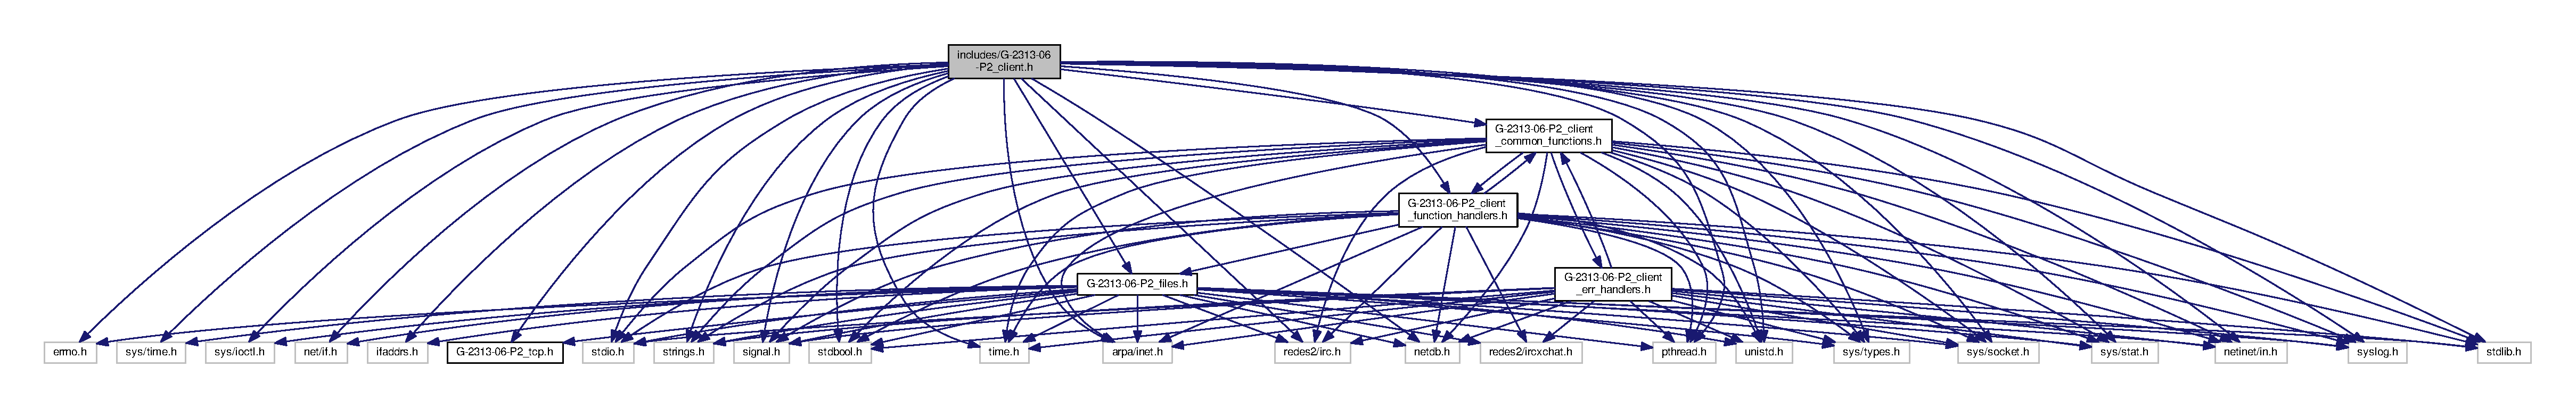
\includegraphics[width=350pt]{G-2313-06-P2__client_8h__incl}
\end{center}
\end{figure}
Gráfico de los archivos que directa o indirectamente incluyen a este archivo\+:\nopagebreak
\begin{figure}[H]
\begin{center}
\leavevmode
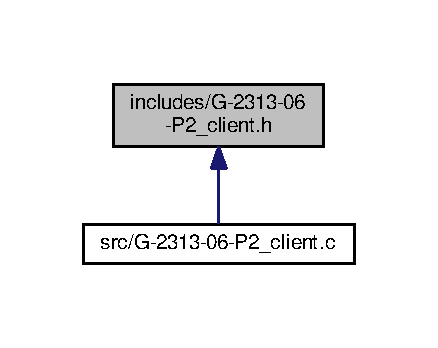
\includegraphics[width=210pt]{G-2313-06-P2__client_8h__dep__incl}
\end{center}
\end{figure}
\subsection*{Funciones}
\begin{DoxyCompactItemize}
\item 
void $\ast$ \hyperlink{G-2313-06-P2__client_8h_a7297f848d5b0bd4990857d03cf3111e4}{client\+\_\+function\+\_\+ping} (void $\ast$arg)
\item 
void $\ast$ \hyperlink{G-2313-06-P2__client_8h_afbd2dc7b3224fc3d2c5c9233b307c376}{client\+\_\+function\+\_\+response} (void $\ast$arg)
\item 
void \hyperlink{G-2313-06-P2__client_8h_aa74c686c447b275e6a8cf36419033e81}{client\+\_\+pre\+\_\+in\+\_\+function} (char $\ast$command)
\item 
void \hyperlink{G-2313-06-P2__client_8h_a6dd72e0b56b87f85d8cac2a30066198b}{client\+\_\+execute\+\_\+in\+\_\+function} (long function\+Name, char $\ast$command)
\item 
void \hyperlink{G-2313-06-P2__client_8h_a68019fe1e0edcc71bb3dadeb70a86dcd}{client\+\_\+pre\+\_\+out\+\_\+function} (char $\ast$command)
\item 
void \hyperlink{G-2313-06-P2__client_8h_a26512d35b24fec46c8fa4c803dc00867}{client\+\_\+execute\+\_\+out\+\_\+function} (long function\+Name, char $\ast$command)
\end{DoxyCompactItemize}


\subsection{Documentación de las funciones}
\index{G-\/2313-\/06-\/\+P2\+\_\+client.\+h@{G-\/2313-\/06-\/\+P2\+\_\+client.\+h}!client\+\_\+execute\+\_\+in\+\_\+function@{client\+\_\+execute\+\_\+in\+\_\+function}}
\index{client\+\_\+execute\+\_\+in\+\_\+function@{client\+\_\+execute\+\_\+in\+\_\+function}!G-\/2313-\/06-\/\+P2\+\_\+client.\+h@{G-\/2313-\/06-\/\+P2\+\_\+client.\+h}}
\subsubsection[{\texorpdfstring{client\+\_\+execute\+\_\+in\+\_\+function(long function\+Name, char $\ast$command)}{client_execute_in_function(long functionName, char *command)}}]{\setlength{\rightskip}{0pt plus 5cm}void client\+\_\+execute\+\_\+in\+\_\+function (
\begin{DoxyParamCaption}
\item[{long}]{function\+Name, }
\item[{char $\ast$}]{command}
\end{DoxyParamCaption}
)}\hypertarget{G-2313-06-P2__client_8h_a6dd72e0b56b87f85d8cac2a30066198b}{}\label{G-2313-06-P2__client_8h_a6dd72e0b56b87f85d8cac2a30066198b}


Definición en la línea 403 del archivo G-\/2313-\/06-\/\+P2\+\_\+client\+\_\+common\+\_\+functions.\+c.

\index{G-\/2313-\/06-\/\+P2\+\_\+client.\+h@{G-\/2313-\/06-\/\+P2\+\_\+client.\+h}!client\+\_\+execute\+\_\+out\+\_\+function@{client\+\_\+execute\+\_\+out\+\_\+function}}
\index{client\+\_\+execute\+\_\+out\+\_\+function@{client\+\_\+execute\+\_\+out\+\_\+function}!G-\/2313-\/06-\/\+P2\+\_\+client.\+h@{G-\/2313-\/06-\/\+P2\+\_\+client.\+h}}
\subsubsection[{\texorpdfstring{client\+\_\+execute\+\_\+out\+\_\+function(long function\+Name, char $\ast$command)}{client_execute_out_function(long functionName, char *command)}}]{\setlength{\rightskip}{0pt plus 5cm}void client\+\_\+execute\+\_\+out\+\_\+function (
\begin{DoxyParamCaption}
\item[{long}]{function\+Name, }
\item[{char $\ast$}]{command}
\end{DoxyParamCaption}
)}\hypertarget{G-2313-06-P2__client_8h_a26512d35b24fec46c8fa4c803dc00867}{}\label{G-2313-06-P2__client_8h_a26512d35b24fec46c8fa4c803dc00867}


Definición en la línea 565 del archivo G-\/2313-\/06-\/\+P2\+\_\+client\+\_\+common\+\_\+functions.\+c.

\index{G-\/2313-\/06-\/\+P2\+\_\+client.\+h@{G-\/2313-\/06-\/\+P2\+\_\+client.\+h}!client\+\_\+function\+\_\+ping@{client\+\_\+function\+\_\+ping}}
\index{client\+\_\+function\+\_\+ping@{client\+\_\+function\+\_\+ping}!G-\/2313-\/06-\/\+P2\+\_\+client.\+h@{G-\/2313-\/06-\/\+P2\+\_\+client.\+h}}
\subsubsection[{\texorpdfstring{client\+\_\+function\+\_\+ping(void $\ast$arg)}{client_function_ping(void *arg)}}]{\setlength{\rightskip}{0pt plus 5cm}void$\ast$ client\+\_\+function\+\_\+ping (
\begin{DoxyParamCaption}
\item[{void $\ast$}]{arg}
\end{DoxyParamCaption}
)}\hypertarget{G-2313-06-P2__client_8h_a7297f848d5b0bd4990857d03cf3111e4}{}\label{G-2313-06-P2__client_8h_a7297f848d5b0bd4990857d03cf3111e4}


Definición en la línea 185 del archivo G-\/2313-\/06-\/\+P2\+\_\+client\+\_\+common\+\_\+functions.\+c.

\index{G-\/2313-\/06-\/\+P2\+\_\+client.\+h@{G-\/2313-\/06-\/\+P2\+\_\+client.\+h}!client\+\_\+function\+\_\+response@{client\+\_\+function\+\_\+response}}
\index{client\+\_\+function\+\_\+response@{client\+\_\+function\+\_\+response}!G-\/2313-\/06-\/\+P2\+\_\+client.\+h@{G-\/2313-\/06-\/\+P2\+\_\+client.\+h}}
\subsubsection[{\texorpdfstring{client\+\_\+function\+\_\+response(void $\ast$arg)}{client_function_response(void *arg)}}]{\setlength{\rightskip}{0pt plus 5cm}void$\ast$ client\+\_\+function\+\_\+response (
\begin{DoxyParamCaption}
\item[{void $\ast$}]{arg}
\end{DoxyParamCaption}
)}\hypertarget{G-2313-06-P2__client_8h_afbd2dc7b3224fc3d2c5c9233b307c376}{}\label{G-2313-06-P2__client_8h_afbd2dc7b3224fc3d2c5c9233b307c376}


Definición en la línea 237 del archivo G-\/2313-\/06-\/\+P2\+\_\+client\+\_\+common\+\_\+functions.\+c.

\index{G-\/2313-\/06-\/\+P2\+\_\+client.\+h@{G-\/2313-\/06-\/\+P2\+\_\+client.\+h}!client\+\_\+pre\+\_\+in\+\_\+function@{client\+\_\+pre\+\_\+in\+\_\+function}}
\index{client\+\_\+pre\+\_\+in\+\_\+function@{client\+\_\+pre\+\_\+in\+\_\+function}!G-\/2313-\/06-\/\+P2\+\_\+client.\+h@{G-\/2313-\/06-\/\+P2\+\_\+client.\+h}}
\subsubsection[{\texorpdfstring{client\+\_\+pre\+\_\+in\+\_\+function(char $\ast$command)}{client_pre_in_function(char *command)}}]{\setlength{\rightskip}{0pt plus 5cm}void client\+\_\+pre\+\_\+in\+\_\+function (
\begin{DoxyParamCaption}
\item[{char $\ast$}]{command}
\end{DoxyParamCaption}
)}\hypertarget{G-2313-06-P2__client_8h_aa74c686c447b275e6a8cf36419033e81}{}\label{G-2313-06-P2__client_8h_aa74c686c447b275e6a8cf36419033e81}


Definición en la línea 306 del archivo G-\/2313-\/06-\/\+P2\+\_\+client\+\_\+common\+\_\+functions.\+c.

\index{G-\/2313-\/06-\/\+P2\+\_\+client.\+h@{G-\/2313-\/06-\/\+P2\+\_\+client.\+h}!client\+\_\+pre\+\_\+out\+\_\+function@{client\+\_\+pre\+\_\+out\+\_\+function}}
\index{client\+\_\+pre\+\_\+out\+\_\+function@{client\+\_\+pre\+\_\+out\+\_\+function}!G-\/2313-\/06-\/\+P2\+\_\+client.\+h@{G-\/2313-\/06-\/\+P2\+\_\+client.\+h}}
\subsubsection[{\texorpdfstring{client\+\_\+pre\+\_\+out\+\_\+function(char $\ast$command)}{client_pre_out_function(char *command)}}]{\setlength{\rightskip}{0pt plus 5cm}void client\+\_\+pre\+\_\+out\+\_\+function (
\begin{DoxyParamCaption}
\item[{char $\ast$}]{command}
\end{DoxyParamCaption}
)}\hypertarget{G-2313-06-P2__client_8h_a68019fe1e0edcc71bb3dadeb70a86dcd}{}\label{G-2313-06-P2__client_8h_a68019fe1e0edcc71bb3dadeb70a86dcd}


Definición en la línea 511 del archivo G-\/2313-\/06-\/\+P2\+\_\+client\+\_\+common\+\_\+functions.\+c.


\hypertarget{G-2313-06-P2__client__common__functions_8h}{}\section{Referencia del Archivo includes/\+G-\/2313-\/06-\/\+P2\+\_\+client\+\_\+common\+\_\+functions.h}
\label{G-2313-06-P2__client__common__functions_8h}\index{includes/\+G-\/2313-\/06-\/\+P2\+\_\+client\+\_\+common\+\_\+functions.\+h@{includes/\+G-\/2313-\/06-\/\+P2\+\_\+client\+\_\+common\+\_\+functions.\+h}}
{\ttfamily \#include $<$unistd.\+h$>$}\\*
{\ttfamily \#include $<$sys/types.\+h$>$}\\*
{\ttfamily \#include $<$sys/socket.\+h$>$}\\*
{\ttfamily \#include $<$sys/stat.\+h$>$}\\*
{\ttfamily \#include $<$netinet/in.\+h$>$}\\*
{\ttfamily \#include $<$syslog.\+h$>$}\\*
{\ttfamily \#include $<$stdlib.\+h$>$}\\*
{\ttfamily \#include $<$stdio.\+h$>$}\\*
{\ttfamily \#include $<$strings.\+h$>$}\\*
{\ttfamily \#include $<$signal.\+h$>$}\\*
{\ttfamily \#include $<$stdbool.\+h$>$}\\*
{\ttfamily \#include $<$time.\+h$>$}\\*
{\ttfamily \#include $<$arpa/inet.\+h$>$}\\*
{\ttfamily \#include $<$redes2/irc.\+h$>$}\\*
{\ttfamily \#include $<$netdb.\+h$>$}\\*
{\ttfamily \#include $<$pthread.\+h$>$}\\*
{\ttfamily \#include \char`\"{}G-\/2313-\/06-\/\+P2\+\_\+client\+\_\+function\+\_\+handlers.\+h\char`\"{}}\\*
{\ttfamily \#include \char`\"{}G-\/2313-\/06-\/\+P2\+\_\+client\+\_\+err\+\_\+handlers.\+h\char`\"{}}\\*
Dependencia gráfica adjunta para G-\/2313-\/06-\/\+P2\+\_\+client\+\_\+common\+\_\+functions.h\+:\nopagebreak
\begin{figure}[H]
\begin{center}
\leavevmode
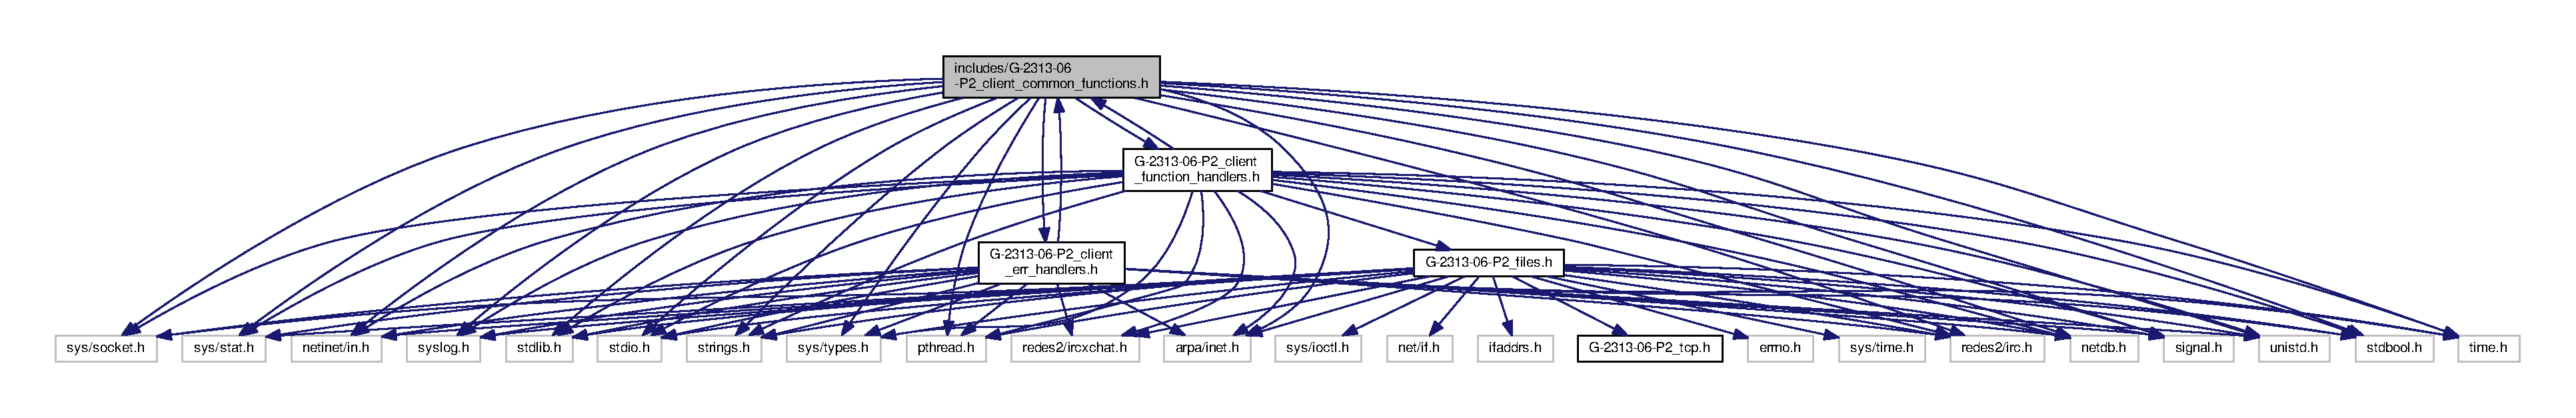
\includegraphics[width=350pt]{G-2313-06-P2__client__common__functions_8h__incl}
\end{center}
\end{figure}
Gráfico de los archivos que directa o indirectamente incluyen a este archivo\+:\nopagebreak
\begin{figure}[H]
\begin{center}
\leavevmode
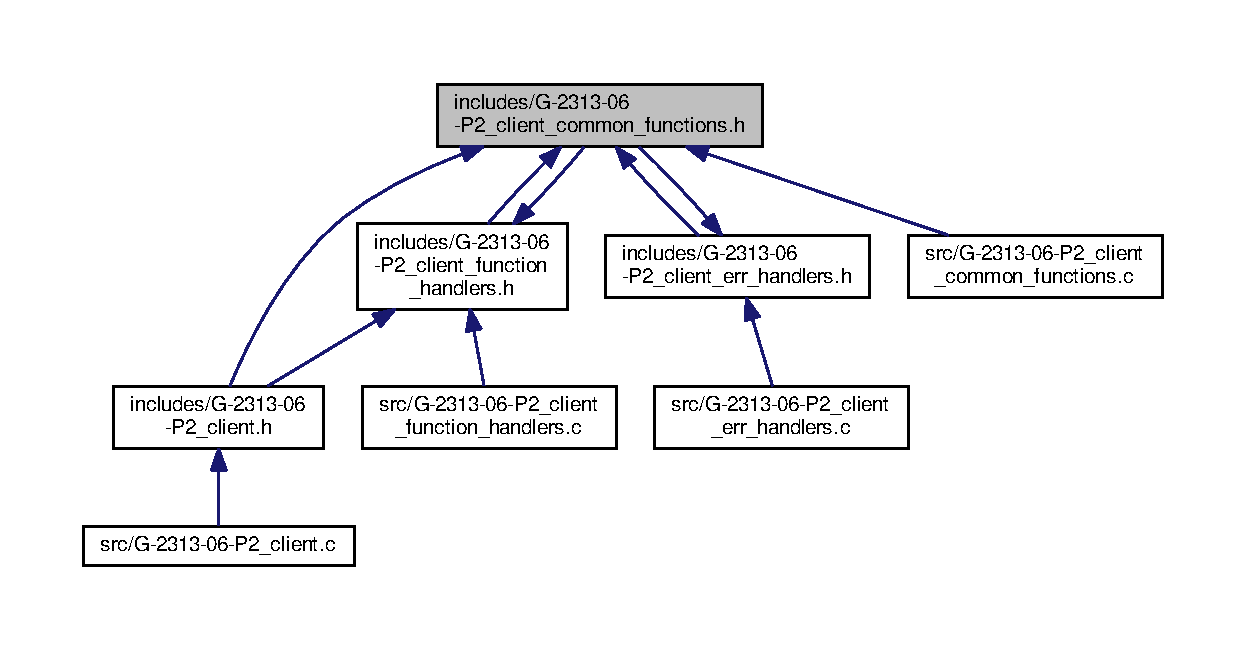
\includegraphics[width=350pt]{G-2313-06-P2__client__common__functions_8h__dep__incl}
\end{center}
\end{figure}
\subsection*{Funciones}
\begin{DoxyCompactItemize}
\item 
void $\ast$ \hyperlink{G-2313-06-P2__client__common__functions_8h_a7297f848d5b0bd4990857d03cf3111e4}{client\+\_\+function\+\_\+ping} (void $\ast$arg)
\item 
void $\ast$ \hyperlink{G-2313-06-P2__client__common__functions_8h_afbd2dc7b3224fc3d2c5c9233b307c376}{client\+\_\+function\+\_\+response} (void $\ast$arg)
\item 
void \hyperlink{G-2313-06-P2__client__common__functions_8h_a03942275c5a503be4f7288cda71fb139}{client\+\_\+show\+\_\+error} (char $\ast$msg)
\item 
void \hyperlink{G-2313-06-P2__client__common__functions_8h_aa74c686c447b275e6a8cf36419033e81}{client\+\_\+pre\+\_\+in\+\_\+function} (char $\ast$command)
\item 
void \hyperlink{G-2313-06-P2__client__common__functions_8h_a6dd72e0b56b87f85d8cac2a30066198b}{client\+\_\+execute\+\_\+in\+\_\+function} (long function\+Name, char $\ast$command)
\item 
void \hyperlink{G-2313-06-P2__client__common__functions_8h_a68019fe1e0edcc71bb3dadeb70a86dcd}{client\+\_\+pre\+\_\+out\+\_\+function} (char $\ast$command)
\item 
void \hyperlink{G-2313-06-P2__client__common__functions_8h_a26512d35b24fec46c8fa4c803dc00867}{client\+\_\+execute\+\_\+out\+\_\+function} (long function\+Name, char $\ast$command)
\end{DoxyCompactItemize}


\subsection{Documentación de las funciones}
\index{G-\/2313-\/06-\/\+P2\+\_\+client\+\_\+common\+\_\+functions.\+h@{G-\/2313-\/06-\/\+P2\+\_\+client\+\_\+common\+\_\+functions.\+h}!client\+\_\+execute\+\_\+in\+\_\+function@{client\+\_\+execute\+\_\+in\+\_\+function}}
\index{client\+\_\+execute\+\_\+in\+\_\+function@{client\+\_\+execute\+\_\+in\+\_\+function}!G-\/2313-\/06-\/\+P2\+\_\+client\+\_\+common\+\_\+functions.\+h@{G-\/2313-\/06-\/\+P2\+\_\+client\+\_\+common\+\_\+functions.\+h}}
\subsubsection[{\texorpdfstring{client\+\_\+execute\+\_\+in\+\_\+function(long function\+Name, char $\ast$command)}{client_execute_in_function(long functionName, char *command)}}]{\setlength{\rightskip}{0pt plus 5cm}void client\+\_\+execute\+\_\+in\+\_\+function (
\begin{DoxyParamCaption}
\item[{long}]{function\+Name, }
\item[{char $\ast$}]{command}
\end{DoxyParamCaption}
)}\hypertarget{G-2313-06-P2__client__common__functions_8h_a6dd72e0b56b87f85d8cac2a30066198b}{}\label{G-2313-06-P2__client__common__functions_8h_a6dd72e0b56b87f85d8cac2a30066198b}


Definición en la línea 67 del archivo G-\/2313-\/06-\/\+P2\+\_\+client\+\_\+common\+\_\+functions.\+c.

\index{G-\/2313-\/06-\/\+P2\+\_\+client\+\_\+common\+\_\+functions.\+h@{G-\/2313-\/06-\/\+P2\+\_\+client\+\_\+common\+\_\+functions.\+h}!client\+\_\+execute\+\_\+out\+\_\+function@{client\+\_\+execute\+\_\+out\+\_\+function}}
\index{client\+\_\+execute\+\_\+out\+\_\+function@{client\+\_\+execute\+\_\+out\+\_\+function}!G-\/2313-\/06-\/\+P2\+\_\+client\+\_\+common\+\_\+functions.\+h@{G-\/2313-\/06-\/\+P2\+\_\+client\+\_\+common\+\_\+functions.\+h}}
\subsubsection[{\texorpdfstring{client\+\_\+execute\+\_\+out\+\_\+function(long function\+Name, char $\ast$command)}{client_execute_out_function(long functionName, char *command)}}]{\setlength{\rightskip}{0pt plus 5cm}void client\+\_\+execute\+\_\+out\+\_\+function (
\begin{DoxyParamCaption}
\item[{long}]{function\+Name, }
\item[{char $\ast$}]{command}
\end{DoxyParamCaption}
)}\hypertarget{G-2313-06-P2__client__common__functions_8h_a26512d35b24fec46c8fa4c803dc00867}{}\label{G-2313-06-P2__client__common__functions_8h_a26512d35b24fec46c8fa4c803dc00867}


Definición en la línea 151 del archivo G-\/2313-\/06-\/\+P2\+\_\+client\+\_\+common\+\_\+functions.\+c.

\index{G-\/2313-\/06-\/\+P2\+\_\+client\+\_\+common\+\_\+functions.\+h@{G-\/2313-\/06-\/\+P2\+\_\+client\+\_\+common\+\_\+functions.\+h}!client\+\_\+function\+\_\+ping@{client\+\_\+function\+\_\+ping}}
\index{client\+\_\+function\+\_\+ping@{client\+\_\+function\+\_\+ping}!G-\/2313-\/06-\/\+P2\+\_\+client\+\_\+common\+\_\+functions.\+h@{G-\/2313-\/06-\/\+P2\+\_\+client\+\_\+common\+\_\+functions.\+h}}
\subsubsection[{\texorpdfstring{client\+\_\+function\+\_\+ping(void $\ast$arg)}{client_function_ping(void *arg)}}]{\setlength{\rightskip}{0pt plus 5cm}void$\ast$ client\+\_\+function\+\_\+ping (
\begin{DoxyParamCaption}
\item[{void $\ast$}]{arg}
\end{DoxyParamCaption}
)}\hypertarget{G-2313-06-P2__client__common__functions_8h_a7297f848d5b0bd4990857d03cf3111e4}{}\label{G-2313-06-P2__client__common__functions_8h_a7297f848d5b0bd4990857d03cf3111e4}


Definición en la línea 5 del archivo G-\/2313-\/06-\/\+P2\+\_\+client\+\_\+common\+\_\+functions.\+c.

\index{G-\/2313-\/06-\/\+P2\+\_\+client\+\_\+common\+\_\+functions.\+h@{G-\/2313-\/06-\/\+P2\+\_\+client\+\_\+common\+\_\+functions.\+h}!client\+\_\+function\+\_\+response@{client\+\_\+function\+\_\+response}}
\index{client\+\_\+function\+\_\+response@{client\+\_\+function\+\_\+response}!G-\/2313-\/06-\/\+P2\+\_\+client\+\_\+common\+\_\+functions.\+h@{G-\/2313-\/06-\/\+P2\+\_\+client\+\_\+common\+\_\+functions.\+h}}
\subsubsection[{\texorpdfstring{client\+\_\+function\+\_\+response(void $\ast$arg)}{client_function_response(void *arg)}}]{\setlength{\rightskip}{0pt plus 5cm}void$\ast$ client\+\_\+function\+\_\+response (
\begin{DoxyParamCaption}
\item[{void $\ast$}]{arg}
\end{DoxyParamCaption}
)}\hypertarget{G-2313-06-P2__client__common__functions_8h_afbd2dc7b3224fc3d2c5c9233b307c376}{}\label{G-2313-06-P2__client__common__functions_8h_afbd2dc7b3224fc3d2c5c9233b307c376}


Definición en la línea 23 del archivo G-\/2313-\/06-\/\+P2\+\_\+client\+\_\+common\+\_\+functions.\+c.

\index{G-\/2313-\/06-\/\+P2\+\_\+client\+\_\+common\+\_\+functions.\+h@{G-\/2313-\/06-\/\+P2\+\_\+client\+\_\+common\+\_\+functions.\+h}!client\+\_\+pre\+\_\+in\+\_\+function@{client\+\_\+pre\+\_\+in\+\_\+function}}
\index{client\+\_\+pre\+\_\+in\+\_\+function@{client\+\_\+pre\+\_\+in\+\_\+function}!G-\/2313-\/06-\/\+P2\+\_\+client\+\_\+common\+\_\+functions.\+h@{G-\/2313-\/06-\/\+P2\+\_\+client\+\_\+common\+\_\+functions.\+h}}
\subsubsection[{\texorpdfstring{client\+\_\+pre\+\_\+in\+\_\+function(char $\ast$command)}{client_pre_in_function(char *command)}}]{\setlength{\rightskip}{0pt plus 5cm}void client\+\_\+pre\+\_\+in\+\_\+function (
\begin{DoxyParamCaption}
\item[{char $\ast$}]{command}
\end{DoxyParamCaption}
)}\hypertarget{G-2313-06-P2__client__common__functions_8h_aa74c686c447b275e6a8cf36419033e81}{}\label{G-2313-06-P2__client__common__functions_8h_aa74c686c447b275e6a8cf36419033e81}


Definición en la línea 63 del archivo G-\/2313-\/06-\/\+P2\+\_\+client\+\_\+common\+\_\+functions.\+c.

\index{G-\/2313-\/06-\/\+P2\+\_\+client\+\_\+common\+\_\+functions.\+h@{G-\/2313-\/06-\/\+P2\+\_\+client\+\_\+common\+\_\+functions.\+h}!client\+\_\+pre\+\_\+out\+\_\+function@{client\+\_\+pre\+\_\+out\+\_\+function}}
\index{client\+\_\+pre\+\_\+out\+\_\+function@{client\+\_\+pre\+\_\+out\+\_\+function}!G-\/2313-\/06-\/\+P2\+\_\+client\+\_\+common\+\_\+functions.\+h@{G-\/2313-\/06-\/\+P2\+\_\+client\+\_\+common\+\_\+functions.\+h}}
\subsubsection[{\texorpdfstring{client\+\_\+pre\+\_\+out\+\_\+function(char $\ast$command)}{client_pre_out_function(char *command)}}]{\setlength{\rightskip}{0pt plus 5cm}void client\+\_\+pre\+\_\+out\+\_\+function (
\begin{DoxyParamCaption}
\item[{char $\ast$}]{command}
\end{DoxyParamCaption}
)}\hypertarget{G-2313-06-P2__client__common__functions_8h_a68019fe1e0edcc71bb3dadeb70a86dcd}{}\label{G-2313-06-P2__client__common__functions_8h_a68019fe1e0edcc71bb3dadeb70a86dcd}


Definición en la línea 146 del archivo G-\/2313-\/06-\/\+P2\+\_\+client\+\_\+common\+\_\+functions.\+c.

\index{G-\/2313-\/06-\/\+P2\+\_\+client\+\_\+common\+\_\+functions.\+h@{G-\/2313-\/06-\/\+P2\+\_\+client\+\_\+common\+\_\+functions.\+h}!client\+\_\+show\+\_\+error@{client\+\_\+show\+\_\+error}}
\index{client\+\_\+show\+\_\+error@{client\+\_\+show\+\_\+error}!G-\/2313-\/06-\/\+P2\+\_\+client\+\_\+common\+\_\+functions.\+h@{G-\/2313-\/06-\/\+P2\+\_\+client\+\_\+common\+\_\+functions.\+h}}
\subsubsection[{\texorpdfstring{client\+\_\+show\+\_\+error(char $\ast$msg)}{client_show_error(char *msg)}}]{\setlength{\rightskip}{0pt plus 5cm}void client\+\_\+show\+\_\+error (
\begin{DoxyParamCaption}
\item[{char $\ast$}]{msg}
\end{DoxyParamCaption}
)}\hypertarget{G-2313-06-P2__client__common__functions_8h_a03942275c5a503be4f7288cda71fb139}{}\label{G-2313-06-P2__client__common__functions_8h_a03942275c5a503be4f7288cda71fb139}


Definición en la línea 53 del archivo G-\/2313-\/06-\/\+P2\+\_\+client\+\_\+common\+\_\+functions.\+c.


\hypertarget{G-2313-06-P2__client__err__handlers_8h}{}\section{Referencia del Archivo includes/\+G-\/2313-\/06-\/\+P2\+\_\+client\+\_\+err\+\_\+handlers.h}
\label{G-2313-06-P2__client__err__handlers_8h}\index{includes/\+G-\/2313-\/06-\/\+P2\+\_\+client\+\_\+err\+\_\+handlers.\+h@{includes/\+G-\/2313-\/06-\/\+P2\+\_\+client\+\_\+err\+\_\+handlers.\+h}}
{\ttfamily \#include $<$unistd.\+h$>$}\\*
{\ttfamily \#include $<$sys/types.\+h$>$}\\*
{\ttfamily \#include $<$sys/socket.\+h$>$}\\*
{\ttfamily \#include $<$sys/stat.\+h$>$}\\*
{\ttfamily \#include $<$netinet/in.\+h$>$}\\*
{\ttfamily \#include $<$syslog.\+h$>$}\\*
{\ttfamily \#include $<$stdlib.\+h$>$}\\*
{\ttfamily \#include $<$stdio.\+h$>$}\\*
{\ttfamily \#include $<$strings.\+h$>$}\\*
{\ttfamily \#include $<$signal.\+h$>$}\\*
{\ttfamily \#include $<$stdbool.\+h$>$}\\*
{\ttfamily \#include $<$time.\+h$>$}\\*
{\ttfamily \#include $<$arpa/inet.\+h$>$}\\*
{\ttfamily \#include $<$redes2/irc.\+h$>$}\\*
{\ttfamily \#include $<$redes2/ircxchat.\+h$>$}\\*
{\ttfamily \#include $<$netdb.\+h$>$}\\*
{\ttfamily \#include $<$pthread.\+h$>$}\\*
{\ttfamily \#include \char`\"{}G-\/2313-\/06-\/\+P2\+\_\+client\+\_\+common\+\_\+functions.\+h\char`\"{}}\\*
Dependencia gráfica adjunta para G-\/2313-\/06-\/\+P2\+\_\+client\+\_\+err\+\_\+handlers.h\+:\nopagebreak
\begin{figure}[H]
\begin{center}
\leavevmode
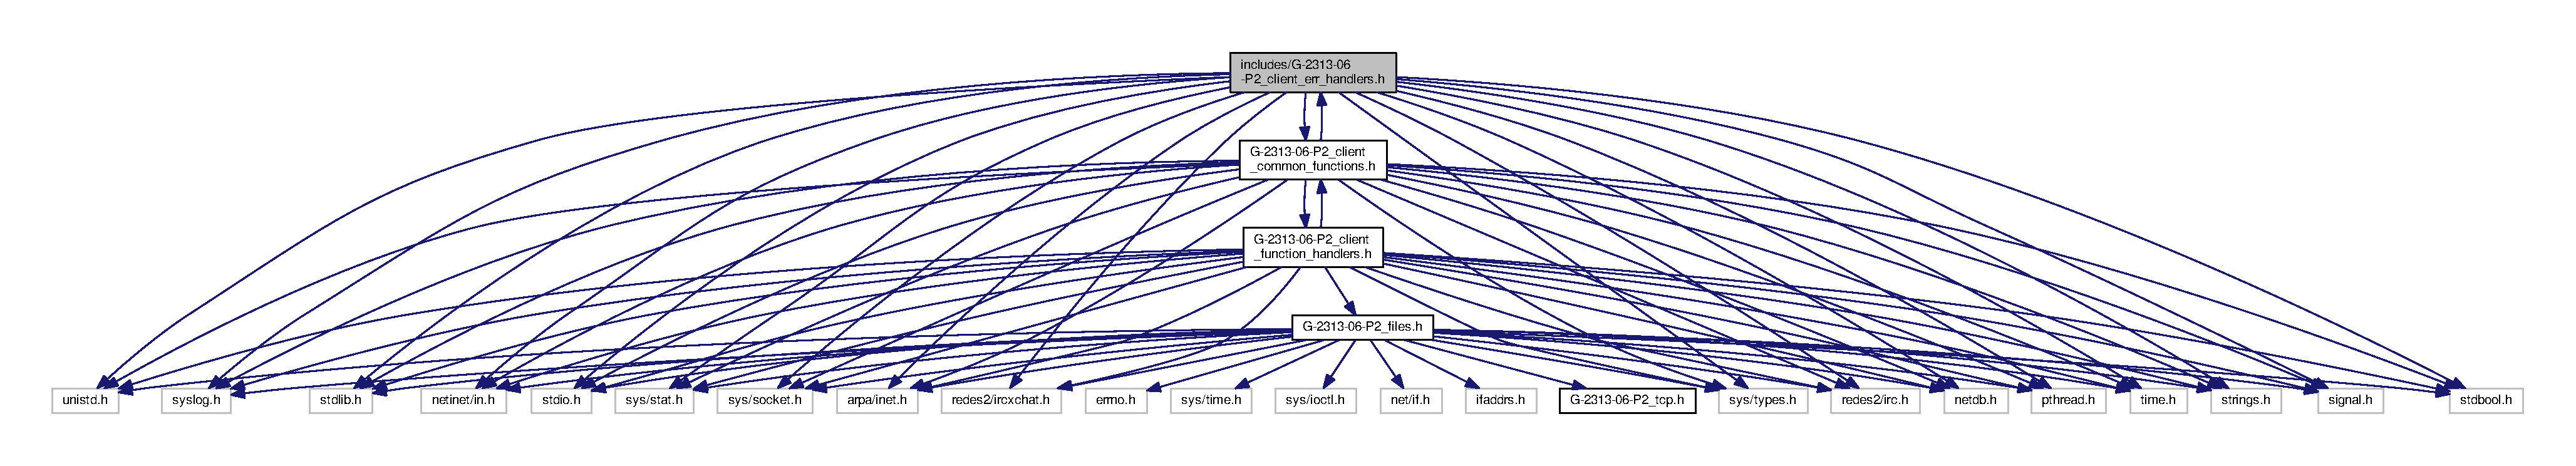
\includegraphics[width=350pt]{G-2313-06-P2__client__err__handlers_8h__incl}
\end{center}
\end{figure}
Gráfico de los archivos que directa o indirectamente incluyen a este archivo\+:\nopagebreak
\begin{figure}[H]
\begin{center}
\leavevmode
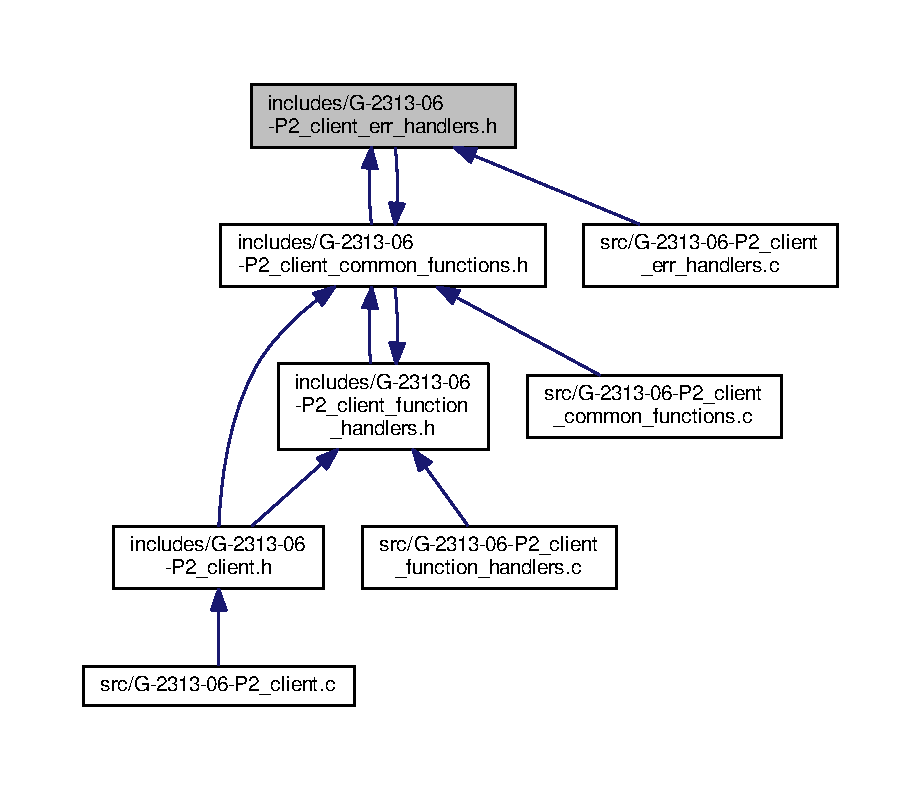
\includegraphics[width=350pt]{G-2313-06-P2__client__err__handlers_8h__dep__incl}
\end{center}
\end{figure}
\subsection*{Funciones}
\begin{DoxyCompactItemize}
\item 
void \hyperlink{G-2313-06-P2__client__err__handlers_8h_aee5973ae831d1c7c63b1a62b59f561c2}{server\+\_\+in\+\_\+command\+\_\+err\+\_\+cannotsendtochan} (char $\ast$command)
\item 
void \hyperlink{G-2313-06-P2__client__err__handlers_8h_a14bfb17eb95d0f2bef1869aa2ebf520c}{server\+\_\+in\+\_\+command\+\_\+err\+\_\+alreadyregistred} (char $\ast$command)
\item 
void \hyperlink{G-2313-06-P2__client__err__handlers_8h_aaa9cfb1b5050bd1218c227d8d0a041fe}{server\+\_\+in\+\_\+command\+\_\+err\+\_\+nonicknamegiven} (char $\ast$command)
\item 
void \hyperlink{G-2313-06-P2__client__err__handlers_8h_abeb8ead21ebba982eb59f161eda735cb}{server\+\_\+in\+\_\+command\+\_\+err\+\_\+erroneusnickname} (char $\ast$command)
\item 
void \hyperlink{G-2313-06-P2__client__err__handlers_8h_ab6d8f2d05566bf6ee9dfcfc4a20f5d23}{server\+\_\+in\+\_\+command\+\_\+err\+\_\+nicknameinuse} (char $\ast$command)
\item 
void \hyperlink{G-2313-06-P2__client__err__handlers_8h_a4af95b292b293c08c0989b4e7334c7eb}{server\+\_\+in\+\_\+command\+\_\+err\+\_\+nickcollision} (char $\ast$command)
\item 
void \hyperlink{G-2313-06-P2__client__err__handlers_8h_ae4fcb567dc7685f5d7a4abbc7c6506b4}{server\+\_\+in\+\_\+command\+\_\+err\+\_\+unavailresource} (char $\ast$command)
\item 
void \hyperlink{G-2313-06-P2__client__err__handlers_8h_ada432444f58d5effbb05fd558a8ce289}{server\+\_\+in\+\_\+command\+\_\+err\+\_\+restricted} (char $\ast$command)
\item 
void \hyperlink{G-2313-06-P2__client__err__handlers_8h_a548a7ad35236521dca4b829e466f3379}{server\+\_\+in\+\_\+command\+\_\+err\+\_\+passwdmismatch} (char $\ast$command)
\item 
void \hyperlink{G-2313-06-P2__client__err__handlers_8h_a0e4059ef132eaac2218fdd89b20ca852}{server\+\_\+in\+\_\+command\+\_\+err\+\_\+bannedfromchan} (char $\ast$command)
\item 
void \hyperlink{G-2313-06-P2__client__err__handlers_8h_a05db0aa32f2ec2925cba3b952435bf59}{server\+\_\+in\+\_\+command\+\_\+err\+\_\+channelisfull} (char $\ast$command)
\item 
void \hyperlink{G-2313-06-P2__client__err__handlers_8h_a9fcb3f66fbcc994c7a78b36ebc0fe63d}{server\+\_\+in\+\_\+command\+\_\+err\+\_\+chanoprivsneeded} (char $\ast$command)
\item 
void \hyperlink{G-2313-06-P2__client__err__handlers_8h_ae5512c3dd8e1584fd8bafc4f5dd15d8c}{server\+\_\+in\+\_\+command\+\_\+err\+\_\+inviteonlychan} (char $\ast$command)
\item 
void \hyperlink{G-2313-06-P2__client__err__handlers_8h_aade31864807344a9961ffdab697b5727}{server\+\_\+in\+\_\+command\+\_\+err\+\_\+nochanmodes} (char $\ast$command)
\item 
void \hyperlink{G-2313-06-P2__client__err__handlers_8h_a83109e15e2a8f93c9523a84a546098c0}{server\+\_\+in\+\_\+command\+\_\+err\+\_\+nosuchchannel} (char $\ast$command)
\item 
void \hyperlink{G-2313-06-P2__client__err__handlers_8h_af262f3569e06c21e3e466266fa4e2c80}{server\+\_\+in\+\_\+command\+\_\+err\+\_\+unknownmode} (char $\ast$command)
\item 
void \hyperlink{G-2313-06-P2__client__err__handlers_8h_a678f368edc1fd437f5f115ef897bdcd9}{server\+\_\+in\+\_\+command\+\_\+err\+\_\+nomotd} (char $\ast$command)
\item 
void \hyperlink{G-2313-06-P2__client__err__handlers_8h_a01f8c9822aac18d5424ebbaf67c06a51}{server\+\_\+in\+\_\+command\+\_\+err\+\_\+nosuchnick} (char $\ast$command)
\end{DoxyCompactItemize}


\subsection{Documentación de las funciones}
\index{G-\/2313-\/06-\/\+P2\+\_\+client\+\_\+err\+\_\+handlers.\+h@{G-\/2313-\/06-\/\+P2\+\_\+client\+\_\+err\+\_\+handlers.\+h}!server\+\_\+in\+\_\+command\+\_\+err\+\_\+alreadyregistred@{server\+\_\+in\+\_\+command\+\_\+err\+\_\+alreadyregistred}}
\index{server\+\_\+in\+\_\+command\+\_\+err\+\_\+alreadyregistred@{server\+\_\+in\+\_\+command\+\_\+err\+\_\+alreadyregistred}!G-\/2313-\/06-\/\+P2\+\_\+client\+\_\+err\+\_\+handlers.\+h@{G-\/2313-\/06-\/\+P2\+\_\+client\+\_\+err\+\_\+handlers.\+h}}
\subsubsection[{\texorpdfstring{server\+\_\+in\+\_\+command\+\_\+err\+\_\+alreadyregistred(char $\ast$command)}{server_in_command_err_alreadyregistred(char *command)}}]{\setlength{\rightskip}{0pt plus 5cm}void server\+\_\+in\+\_\+command\+\_\+err\+\_\+alreadyregistred (
\begin{DoxyParamCaption}
\item[{char $\ast$}]{command}
\end{DoxyParamCaption}
)}\hypertarget{G-2313-06-P2__client__err__handlers_8h_a14bfb17eb95d0f2bef1869aa2ebf520c}{}\label{G-2313-06-P2__client__err__handlers_8h_a14bfb17eb95d0f2bef1869aa2ebf520c}


Definición en la línea 17 del archivo G-\/2313-\/06-\/\+P2\+\_\+client\+\_\+err\+\_\+handlers.\+c.

\index{G-\/2313-\/06-\/\+P2\+\_\+client\+\_\+err\+\_\+handlers.\+h@{G-\/2313-\/06-\/\+P2\+\_\+client\+\_\+err\+\_\+handlers.\+h}!server\+\_\+in\+\_\+command\+\_\+err\+\_\+bannedfromchan@{server\+\_\+in\+\_\+command\+\_\+err\+\_\+bannedfromchan}}
\index{server\+\_\+in\+\_\+command\+\_\+err\+\_\+bannedfromchan@{server\+\_\+in\+\_\+command\+\_\+err\+\_\+bannedfromchan}!G-\/2313-\/06-\/\+P2\+\_\+client\+\_\+err\+\_\+handlers.\+h@{G-\/2313-\/06-\/\+P2\+\_\+client\+\_\+err\+\_\+handlers.\+h}}
\subsubsection[{\texorpdfstring{server\+\_\+in\+\_\+command\+\_\+err\+\_\+bannedfromchan(char $\ast$command)}{server_in_command_err_bannedfromchan(char *command)}}]{\setlength{\rightskip}{0pt plus 5cm}void server\+\_\+in\+\_\+command\+\_\+err\+\_\+bannedfromchan (
\begin{DoxyParamCaption}
\item[{char $\ast$}]{command}
\end{DoxyParamCaption}
)}\hypertarget{G-2313-06-P2__client__err__handlers_8h_a0e4059ef132eaac2218fdd89b20ca852}{}\label{G-2313-06-P2__client__err__handlers_8h_a0e4059ef132eaac2218fdd89b20ca852}


Definición en la línea 97 del archivo G-\/2313-\/06-\/\+P2\+\_\+client\+\_\+err\+\_\+handlers.\+c.

\index{G-\/2313-\/06-\/\+P2\+\_\+client\+\_\+err\+\_\+handlers.\+h@{G-\/2313-\/06-\/\+P2\+\_\+client\+\_\+err\+\_\+handlers.\+h}!server\+\_\+in\+\_\+command\+\_\+err\+\_\+cannotsendtochan@{server\+\_\+in\+\_\+command\+\_\+err\+\_\+cannotsendtochan}}
\index{server\+\_\+in\+\_\+command\+\_\+err\+\_\+cannotsendtochan@{server\+\_\+in\+\_\+command\+\_\+err\+\_\+cannotsendtochan}!G-\/2313-\/06-\/\+P2\+\_\+client\+\_\+err\+\_\+handlers.\+h@{G-\/2313-\/06-\/\+P2\+\_\+client\+\_\+err\+\_\+handlers.\+h}}
\subsubsection[{\texorpdfstring{server\+\_\+in\+\_\+command\+\_\+err\+\_\+cannotsendtochan(char $\ast$command)}{server_in_command_err_cannotsendtochan(char *command)}}]{\setlength{\rightskip}{0pt plus 5cm}void server\+\_\+in\+\_\+command\+\_\+err\+\_\+cannotsendtochan (
\begin{DoxyParamCaption}
\item[{char $\ast$}]{command}
\end{DoxyParamCaption}
)}\hypertarget{G-2313-06-P2__client__err__handlers_8h_aee5973ae831d1c7c63b1a62b59f561c2}{}\label{G-2313-06-P2__client__err__handlers_8h_aee5973ae831d1c7c63b1a62b59f561c2}


Definición en la línea 7 del archivo G-\/2313-\/06-\/\+P2\+\_\+client\+\_\+err\+\_\+handlers.\+c.

\index{G-\/2313-\/06-\/\+P2\+\_\+client\+\_\+err\+\_\+handlers.\+h@{G-\/2313-\/06-\/\+P2\+\_\+client\+\_\+err\+\_\+handlers.\+h}!server\+\_\+in\+\_\+command\+\_\+err\+\_\+channelisfull@{server\+\_\+in\+\_\+command\+\_\+err\+\_\+channelisfull}}
\index{server\+\_\+in\+\_\+command\+\_\+err\+\_\+channelisfull@{server\+\_\+in\+\_\+command\+\_\+err\+\_\+channelisfull}!G-\/2313-\/06-\/\+P2\+\_\+client\+\_\+err\+\_\+handlers.\+h@{G-\/2313-\/06-\/\+P2\+\_\+client\+\_\+err\+\_\+handlers.\+h}}
\subsubsection[{\texorpdfstring{server\+\_\+in\+\_\+command\+\_\+err\+\_\+channelisfull(char $\ast$command)}{server_in_command_err_channelisfull(char *command)}}]{\setlength{\rightskip}{0pt plus 5cm}void server\+\_\+in\+\_\+command\+\_\+err\+\_\+channelisfull (
\begin{DoxyParamCaption}
\item[{char $\ast$}]{command}
\end{DoxyParamCaption}
)}\hypertarget{G-2313-06-P2__client__err__handlers_8h_a05db0aa32f2ec2925cba3b952435bf59}{}\label{G-2313-06-P2__client__err__handlers_8h_a05db0aa32f2ec2925cba3b952435bf59}


Definición en la línea 107 del archivo G-\/2313-\/06-\/\+P2\+\_\+client\+\_\+err\+\_\+handlers.\+c.

\index{G-\/2313-\/06-\/\+P2\+\_\+client\+\_\+err\+\_\+handlers.\+h@{G-\/2313-\/06-\/\+P2\+\_\+client\+\_\+err\+\_\+handlers.\+h}!server\+\_\+in\+\_\+command\+\_\+err\+\_\+chanoprivsneeded@{server\+\_\+in\+\_\+command\+\_\+err\+\_\+chanoprivsneeded}}
\index{server\+\_\+in\+\_\+command\+\_\+err\+\_\+chanoprivsneeded@{server\+\_\+in\+\_\+command\+\_\+err\+\_\+chanoprivsneeded}!G-\/2313-\/06-\/\+P2\+\_\+client\+\_\+err\+\_\+handlers.\+h@{G-\/2313-\/06-\/\+P2\+\_\+client\+\_\+err\+\_\+handlers.\+h}}
\subsubsection[{\texorpdfstring{server\+\_\+in\+\_\+command\+\_\+err\+\_\+chanoprivsneeded(char $\ast$command)}{server_in_command_err_chanoprivsneeded(char *command)}}]{\setlength{\rightskip}{0pt plus 5cm}void server\+\_\+in\+\_\+command\+\_\+err\+\_\+chanoprivsneeded (
\begin{DoxyParamCaption}
\item[{char $\ast$}]{command}
\end{DoxyParamCaption}
)}\hypertarget{G-2313-06-P2__client__err__handlers_8h_a9fcb3f66fbcc994c7a78b36ebc0fe63d}{}\label{G-2313-06-P2__client__err__handlers_8h_a9fcb3f66fbcc994c7a78b36ebc0fe63d}


Definición en la línea 117 del archivo G-\/2313-\/06-\/\+P2\+\_\+client\+\_\+err\+\_\+handlers.\+c.

\index{G-\/2313-\/06-\/\+P2\+\_\+client\+\_\+err\+\_\+handlers.\+h@{G-\/2313-\/06-\/\+P2\+\_\+client\+\_\+err\+\_\+handlers.\+h}!server\+\_\+in\+\_\+command\+\_\+err\+\_\+erroneusnickname@{server\+\_\+in\+\_\+command\+\_\+err\+\_\+erroneusnickname}}
\index{server\+\_\+in\+\_\+command\+\_\+err\+\_\+erroneusnickname@{server\+\_\+in\+\_\+command\+\_\+err\+\_\+erroneusnickname}!G-\/2313-\/06-\/\+P2\+\_\+client\+\_\+err\+\_\+handlers.\+h@{G-\/2313-\/06-\/\+P2\+\_\+client\+\_\+err\+\_\+handlers.\+h}}
\subsubsection[{\texorpdfstring{server\+\_\+in\+\_\+command\+\_\+err\+\_\+erroneusnickname(char $\ast$command)}{server_in_command_err_erroneusnickname(char *command)}}]{\setlength{\rightskip}{0pt plus 5cm}void server\+\_\+in\+\_\+command\+\_\+err\+\_\+erroneusnickname (
\begin{DoxyParamCaption}
\item[{char $\ast$}]{command}
\end{DoxyParamCaption}
)}\hypertarget{G-2313-06-P2__client__err__handlers_8h_abeb8ead21ebba982eb59f161eda735cb}{}\label{G-2313-06-P2__client__err__handlers_8h_abeb8ead21ebba982eb59f161eda735cb}


Definición en la línea 37 del archivo G-\/2313-\/06-\/\+P2\+\_\+client\+\_\+err\+\_\+handlers.\+c.

\index{G-\/2313-\/06-\/\+P2\+\_\+client\+\_\+err\+\_\+handlers.\+h@{G-\/2313-\/06-\/\+P2\+\_\+client\+\_\+err\+\_\+handlers.\+h}!server\+\_\+in\+\_\+command\+\_\+err\+\_\+inviteonlychan@{server\+\_\+in\+\_\+command\+\_\+err\+\_\+inviteonlychan}}
\index{server\+\_\+in\+\_\+command\+\_\+err\+\_\+inviteonlychan@{server\+\_\+in\+\_\+command\+\_\+err\+\_\+inviteonlychan}!G-\/2313-\/06-\/\+P2\+\_\+client\+\_\+err\+\_\+handlers.\+h@{G-\/2313-\/06-\/\+P2\+\_\+client\+\_\+err\+\_\+handlers.\+h}}
\subsubsection[{\texorpdfstring{server\+\_\+in\+\_\+command\+\_\+err\+\_\+inviteonlychan(char $\ast$command)}{server_in_command_err_inviteonlychan(char *command)}}]{\setlength{\rightskip}{0pt plus 5cm}void server\+\_\+in\+\_\+command\+\_\+err\+\_\+inviteonlychan (
\begin{DoxyParamCaption}
\item[{char $\ast$}]{command}
\end{DoxyParamCaption}
)}\hypertarget{G-2313-06-P2__client__err__handlers_8h_ae5512c3dd8e1584fd8bafc4f5dd15d8c}{}\label{G-2313-06-P2__client__err__handlers_8h_ae5512c3dd8e1584fd8bafc4f5dd15d8c}


Definición en la línea 127 del archivo G-\/2313-\/06-\/\+P2\+\_\+client\+\_\+err\+\_\+handlers.\+c.

\index{G-\/2313-\/06-\/\+P2\+\_\+client\+\_\+err\+\_\+handlers.\+h@{G-\/2313-\/06-\/\+P2\+\_\+client\+\_\+err\+\_\+handlers.\+h}!server\+\_\+in\+\_\+command\+\_\+err\+\_\+nickcollision@{server\+\_\+in\+\_\+command\+\_\+err\+\_\+nickcollision}}
\index{server\+\_\+in\+\_\+command\+\_\+err\+\_\+nickcollision@{server\+\_\+in\+\_\+command\+\_\+err\+\_\+nickcollision}!G-\/2313-\/06-\/\+P2\+\_\+client\+\_\+err\+\_\+handlers.\+h@{G-\/2313-\/06-\/\+P2\+\_\+client\+\_\+err\+\_\+handlers.\+h}}
\subsubsection[{\texorpdfstring{server\+\_\+in\+\_\+command\+\_\+err\+\_\+nickcollision(char $\ast$command)}{server_in_command_err_nickcollision(char *command)}}]{\setlength{\rightskip}{0pt plus 5cm}void server\+\_\+in\+\_\+command\+\_\+err\+\_\+nickcollision (
\begin{DoxyParamCaption}
\item[{char $\ast$}]{command}
\end{DoxyParamCaption}
)}\hypertarget{G-2313-06-P2__client__err__handlers_8h_a4af95b292b293c08c0989b4e7334c7eb}{}\label{G-2313-06-P2__client__err__handlers_8h_a4af95b292b293c08c0989b4e7334c7eb}


Definición en la línea 57 del archivo G-\/2313-\/06-\/\+P2\+\_\+client\+\_\+err\+\_\+handlers.\+c.

\index{G-\/2313-\/06-\/\+P2\+\_\+client\+\_\+err\+\_\+handlers.\+h@{G-\/2313-\/06-\/\+P2\+\_\+client\+\_\+err\+\_\+handlers.\+h}!server\+\_\+in\+\_\+command\+\_\+err\+\_\+nicknameinuse@{server\+\_\+in\+\_\+command\+\_\+err\+\_\+nicknameinuse}}
\index{server\+\_\+in\+\_\+command\+\_\+err\+\_\+nicknameinuse@{server\+\_\+in\+\_\+command\+\_\+err\+\_\+nicknameinuse}!G-\/2313-\/06-\/\+P2\+\_\+client\+\_\+err\+\_\+handlers.\+h@{G-\/2313-\/06-\/\+P2\+\_\+client\+\_\+err\+\_\+handlers.\+h}}
\subsubsection[{\texorpdfstring{server\+\_\+in\+\_\+command\+\_\+err\+\_\+nicknameinuse(char $\ast$command)}{server_in_command_err_nicknameinuse(char *command)}}]{\setlength{\rightskip}{0pt plus 5cm}void server\+\_\+in\+\_\+command\+\_\+err\+\_\+nicknameinuse (
\begin{DoxyParamCaption}
\item[{char $\ast$}]{command}
\end{DoxyParamCaption}
)}\hypertarget{G-2313-06-P2__client__err__handlers_8h_ab6d8f2d05566bf6ee9dfcfc4a20f5d23}{}\label{G-2313-06-P2__client__err__handlers_8h_ab6d8f2d05566bf6ee9dfcfc4a20f5d23}


Definición en la línea 47 del archivo G-\/2313-\/06-\/\+P2\+\_\+client\+\_\+err\+\_\+handlers.\+c.

\index{G-\/2313-\/06-\/\+P2\+\_\+client\+\_\+err\+\_\+handlers.\+h@{G-\/2313-\/06-\/\+P2\+\_\+client\+\_\+err\+\_\+handlers.\+h}!server\+\_\+in\+\_\+command\+\_\+err\+\_\+nochanmodes@{server\+\_\+in\+\_\+command\+\_\+err\+\_\+nochanmodes}}
\index{server\+\_\+in\+\_\+command\+\_\+err\+\_\+nochanmodes@{server\+\_\+in\+\_\+command\+\_\+err\+\_\+nochanmodes}!G-\/2313-\/06-\/\+P2\+\_\+client\+\_\+err\+\_\+handlers.\+h@{G-\/2313-\/06-\/\+P2\+\_\+client\+\_\+err\+\_\+handlers.\+h}}
\subsubsection[{\texorpdfstring{server\+\_\+in\+\_\+command\+\_\+err\+\_\+nochanmodes(char $\ast$command)}{server_in_command_err_nochanmodes(char *command)}}]{\setlength{\rightskip}{0pt plus 5cm}void server\+\_\+in\+\_\+command\+\_\+err\+\_\+nochanmodes (
\begin{DoxyParamCaption}
\item[{char $\ast$}]{command}
\end{DoxyParamCaption}
)}\hypertarget{G-2313-06-P2__client__err__handlers_8h_aade31864807344a9961ffdab697b5727}{}\label{G-2313-06-P2__client__err__handlers_8h_aade31864807344a9961ffdab697b5727}


Definición en la línea 137 del archivo G-\/2313-\/06-\/\+P2\+\_\+client\+\_\+err\+\_\+handlers.\+c.

\index{G-\/2313-\/06-\/\+P2\+\_\+client\+\_\+err\+\_\+handlers.\+h@{G-\/2313-\/06-\/\+P2\+\_\+client\+\_\+err\+\_\+handlers.\+h}!server\+\_\+in\+\_\+command\+\_\+err\+\_\+nomotd@{server\+\_\+in\+\_\+command\+\_\+err\+\_\+nomotd}}
\index{server\+\_\+in\+\_\+command\+\_\+err\+\_\+nomotd@{server\+\_\+in\+\_\+command\+\_\+err\+\_\+nomotd}!G-\/2313-\/06-\/\+P2\+\_\+client\+\_\+err\+\_\+handlers.\+h@{G-\/2313-\/06-\/\+P2\+\_\+client\+\_\+err\+\_\+handlers.\+h}}
\subsubsection[{\texorpdfstring{server\+\_\+in\+\_\+command\+\_\+err\+\_\+nomotd(char $\ast$command)}{server_in_command_err_nomotd(char *command)}}]{\setlength{\rightskip}{0pt plus 5cm}void server\+\_\+in\+\_\+command\+\_\+err\+\_\+nomotd (
\begin{DoxyParamCaption}
\item[{char $\ast$}]{command}
\end{DoxyParamCaption}
)}\hypertarget{G-2313-06-P2__client__err__handlers_8h_a678f368edc1fd437f5f115ef897bdcd9}{}\label{G-2313-06-P2__client__err__handlers_8h_a678f368edc1fd437f5f115ef897bdcd9}


Definición en la línea 167 del archivo G-\/2313-\/06-\/\+P2\+\_\+client\+\_\+err\+\_\+handlers.\+c.

\index{G-\/2313-\/06-\/\+P2\+\_\+client\+\_\+err\+\_\+handlers.\+h@{G-\/2313-\/06-\/\+P2\+\_\+client\+\_\+err\+\_\+handlers.\+h}!server\+\_\+in\+\_\+command\+\_\+err\+\_\+nonicknamegiven@{server\+\_\+in\+\_\+command\+\_\+err\+\_\+nonicknamegiven}}
\index{server\+\_\+in\+\_\+command\+\_\+err\+\_\+nonicknamegiven@{server\+\_\+in\+\_\+command\+\_\+err\+\_\+nonicknamegiven}!G-\/2313-\/06-\/\+P2\+\_\+client\+\_\+err\+\_\+handlers.\+h@{G-\/2313-\/06-\/\+P2\+\_\+client\+\_\+err\+\_\+handlers.\+h}}
\subsubsection[{\texorpdfstring{server\+\_\+in\+\_\+command\+\_\+err\+\_\+nonicknamegiven(char $\ast$command)}{server_in_command_err_nonicknamegiven(char *command)}}]{\setlength{\rightskip}{0pt plus 5cm}void server\+\_\+in\+\_\+command\+\_\+err\+\_\+nonicknamegiven (
\begin{DoxyParamCaption}
\item[{char $\ast$}]{command}
\end{DoxyParamCaption}
)}\hypertarget{G-2313-06-P2__client__err__handlers_8h_aaa9cfb1b5050bd1218c227d8d0a041fe}{}\label{G-2313-06-P2__client__err__handlers_8h_aaa9cfb1b5050bd1218c227d8d0a041fe}


Definición en la línea 27 del archivo G-\/2313-\/06-\/\+P2\+\_\+client\+\_\+err\+\_\+handlers.\+c.

\index{G-\/2313-\/06-\/\+P2\+\_\+client\+\_\+err\+\_\+handlers.\+h@{G-\/2313-\/06-\/\+P2\+\_\+client\+\_\+err\+\_\+handlers.\+h}!server\+\_\+in\+\_\+command\+\_\+err\+\_\+nosuchchannel@{server\+\_\+in\+\_\+command\+\_\+err\+\_\+nosuchchannel}}
\index{server\+\_\+in\+\_\+command\+\_\+err\+\_\+nosuchchannel@{server\+\_\+in\+\_\+command\+\_\+err\+\_\+nosuchchannel}!G-\/2313-\/06-\/\+P2\+\_\+client\+\_\+err\+\_\+handlers.\+h@{G-\/2313-\/06-\/\+P2\+\_\+client\+\_\+err\+\_\+handlers.\+h}}
\subsubsection[{\texorpdfstring{server\+\_\+in\+\_\+command\+\_\+err\+\_\+nosuchchannel(char $\ast$command)}{server_in_command_err_nosuchchannel(char *command)}}]{\setlength{\rightskip}{0pt plus 5cm}void server\+\_\+in\+\_\+command\+\_\+err\+\_\+nosuchchannel (
\begin{DoxyParamCaption}
\item[{char $\ast$}]{command}
\end{DoxyParamCaption}
)}\hypertarget{G-2313-06-P2__client__err__handlers_8h_a83109e15e2a8f93c9523a84a546098c0}{}\label{G-2313-06-P2__client__err__handlers_8h_a83109e15e2a8f93c9523a84a546098c0}


Definición en la línea 147 del archivo G-\/2313-\/06-\/\+P2\+\_\+client\+\_\+err\+\_\+handlers.\+c.

\index{G-\/2313-\/06-\/\+P2\+\_\+client\+\_\+err\+\_\+handlers.\+h@{G-\/2313-\/06-\/\+P2\+\_\+client\+\_\+err\+\_\+handlers.\+h}!server\+\_\+in\+\_\+command\+\_\+err\+\_\+nosuchnick@{server\+\_\+in\+\_\+command\+\_\+err\+\_\+nosuchnick}}
\index{server\+\_\+in\+\_\+command\+\_\+err\+\_\+nosuchnick@{server\+\_\+in\+\_\+command\+\_\+err\+\_\+nosuchnick}!G-\/2313-\/06-\/\+P2\+\_\+client\+\_\+err\+\_\+handlers.\+h@{G-\/2313-\/06-\/\+P2\+\_\+client\+\_\+err\+\_\+handlers.\+h}}
\subsubsection[{\texorpdfstring{server\+\_\+in\+\_\+command\+\_\+err\+\_\+nosuchnick(char $\ast$command)}{server_in_command_err_nosuchnick(char *command)}}]{\setlength{\rightskip}{0pt plus 5cm}void server\+\_\+in\+\_\+command\+\_\+err\+\_\+nosuchnick (
\begin{DoxyParamCaption}
\item[{char $\ast$}]{command}
\end{DoxyParamCaption}
)}\hypertarget{G-2313-06-P2__client__err__handlers_8h_a01f8c9822aac18d5424ebbaf67c06a51}{}\label{G-2313-06-P2__client__err__handlers_8h_a01f8c9822aac18d5424ebbaf67c06a51}


Definición en la línea 177 del archivo G-\/2313-\/06-\/\+P2\+\_\+client\+\_\+err\+\_\+handlers.\+c.

\index{G-\/2313-\/06-\/\+P2\+\_\+client\+\_\+err\+\_\+handlers.\+h@{G-\/2313-\/06-\/\+P2\+\_\+client\+\_\+err\+\_\+handlers.\+h}!server\+\_\+in\+\_\+command\+\_\+err\+\_\+passwdmismatch@{server\+\_\+in\+\_\+command\+\_\+err\+\_\+passwdmismatch}}
\index{server\+\_\+in\+\_\+command\+\_\+err\+\_\+passwdmismatch@{server\+\_\+in\+\_\+command\+\_\+err\+\_\+passwdmismatch}!G-\/2313-\/06-\/\+P2\+\_\+client\+\_\+err\+\_\+handlers.\+h@{G-\/2313-\/06-\/\+P2\+\_\+client\+\_\+err\+\_\+handlers.\+h}}
\subsubsection[{\texorpdfstring{server\+\_\+in\+\_\+command\+\_\+err\+\_\+passwdmismatch(char $\ast$command)}{server_in_command_err_passwdmismatch(char *command)}}]{\setlength{\rightskip}{0pt plus 5cm}void server\+\_\+in\+\_\+command\+\_\+err\+\_\+passwdmismatch (
\begin{DoxyParamCaption}
\item[{char $\ast$}]{command}
\end{DoxyParamCaption}
)}\hypertarget{G-2313-06-P2__client__err__handlers_8h_a548a7ad35236521dca4b829e466f3379}{}\label{G-2313-06-P2__client__err__handlers_8h_a548a7ad35236521dca4b829e466f3379}


Definición en la línea 87 del archivo G-\/2313-\/06-\/\+P2\+\_\+client\+\_\+err\+\_\+handlers.\+c.

\index{G-\/2313-\/06-\/\+P2\+\_\+client\+\_\+err\+\_\+handlers.\+h@{G-\/2313-\/06-\/\+P2\+\_\+client\+\_\+err\+\_\+handlers.\+h}!server\+\_\+in\+\_\+command\+\_\+err\+\_\+restricted@{server\+\_\+in\+\_\+command\+\_\+err\+\_\+restricted}}
\index{server\+\_\+in\+\_\+command\+\_\+err\+\_\+restricted@{server\+\_\+in\+\_\+command\+\_\+err\+\_\+restricted}!G-\/2313-\/06-\/\+P2\+\_\+client\+\_\+err\+\_\+handlers.\+h@{G-\/2313-\/06-\/\+P2\+\_\+client\+\_\+err\+\_\+handlers.\+h}}
\subsubsection[{\texorpdfstring{server\+\_\+in\+\_\+command\+\_\+err\+\_\+restricted(char $\ast$command)}{server_in_command_err_restricted(char *command)}}]{\setlength{\rightskip}{0pt plus 5cm}void server\+\_\+in\+\_\+command\+\_\+err\+\_\+restricted (
\begin{DoxyParamCaption}
\item[{char $\ast$}]{command}
\end{DoxyParamCaption}
)}\hypertarget{G-2313-06-P2__client__err__handlers_8h_ada432444f58d5effbb05fd558a8ce289}{}\label{G-2313-06-P2__client__err__handlers_8h_ada432444f58d5effbb05fd558a8ce289}


Definición en la línea 77 del archivo G-\/2313-\/06-\/\+P2\+\_\+client\+\_\+err\+\_\+handlers.\+c.

\index{G-\/2313-\/06-\/\+P2\+\_\+client\+\_\+err\+\_\+handlers.\+h@{G-\/2313-\/06-\/\+P2\+\_\+client\+\_\+err\+\_\+handlers.\+h}!server\+\_\+in\+\_\+command\+\_\+err\+\_\+unavailresource@{server\+\_\+in\+\_\+command\+\_\+err\+\_\+unavailresource}}
\index{server\+\_\+in\+\_\+command\+\_\+err\+\_\+unavailresource@{server\+\_\+in\+\_\+command\+\_\+err\+\_\+unavailresource}!G-\/2313-\/06-\/\+P2\+\_\+client\+\_\+err\+\_\+handlers.\+h@{G-\/2313-\/06-\/\+P2\+\_\+client\+\_\+err\+\_\+handlers.\+h}}
\subsubsection[{\texorpdfstring{server\+\_\+in\+\_\+command\+\_\+err\+\_\+unavailresource(char $\ast$command)}{server_in_command_err_unavailresource(char *command)}}]{\setlength{\rightskip}{0pt plus 5cm}void server\+\_\+in\+\_\+command\+\_\+err\+\_\+unavailresource (
\begin{DoxyParamCaption}
\item[{char $\ast$}]{command}
\end{DoxyParamCaption}
)}\hypertarget{G-2313-06-P2__client__err__handlers_8h_ae4fcb567dc7685f5d7a4abbc7c6506b4}{}\label{G-2313-06-P2__client__err__handlers_8h_ae4fcb567dc7685f5d7a4abbc7c6506b4}


Definición en la línea 67 del archivo G-\/2313-\/06-\/\+P2\+\_\+client\+\_\+err\+\_\+handlers.\+c.

\index{G-\/2313-\/06-\/\+P2\+\_\+client\+\_\+err\+\_\+handlers.\+h@{G-\/2313-\/06-\/\+P2\+\_\+client\+\_\+err\+\_\+handlers.\+h}!server\+\_\+in\+\_\+command\+\_\+err\+\_\+unknownmode@{server\+\_\+in\+\_\+command\+\_\+err\+\_\+unknownmode}}
\index{server\+\_\+in\+\_\+command\+\_\+err\+\_\+unknownmode@{server\+\_\+in\+\_\+command\+\_\+err\+\_\+unknownmode}!G-\/2313-\/06-\/\+P2\+\_\+client\+\_\+err\+\_\+handlers.\+h@{G-\/2313-\/06-\/\+P2\+\_\+client\+\_\+err\+\_\+handlers.\+h}}
\subsubsection[{\texorpdfstring{server\+\_\+in\+\_\+command\+\_\+err\+\_\+unknownmode(char $\ast$command)}{server_in_command_err_unknownmode(char *command)}}]{\setlength{\rightskip}{0pt plus 5cm}void server\+\_\+in\+\_\+command\+\_\+err\+\_\+unknownmode (
\begin{DoxyParamCaption}
\item[{char $\ast$}]{command}
\end{DoxyParamCaption}
)}\hypertarget{G-2313-06-P2__client__err__handlers_8h_af262f3569e06c21e3e466266fa4e2c80}{}\label{G-2313-06-P2__client__err__handlers_8h_af262f3569e06c21e3e466266fa4e2c80}


Definición en la línea 157 del archivo G-\/2313-\/06-\/\+P2\+\_\+client\+\_\+err\+\_\+handlers.\+c.


\hypertarget{G-2313-06-P2__client__function__handlers_8h}{}\section{Referencia del Archivo includes/\+G-\/2313-\/06-\/\+P2\+\_\+client\+\_\+function\+\_\+handlers.h}
\label{G-2313-06-P2__client__function__handlers_8h}\index{includes/\+G-\/2313-\/06-\/\+P2\+\_\+client\+\_\+function\+\_\+handlers.\+h@{includes/\+G-\/2313-\/06-\/\+P2\+\_\+client\+\_\+function\+\_\+handlers.\+h}}
{\ttfamily \#include $<$unistd.\+h$>$}\\*
{\ttfamily \#include $<$sys/types.\+h$>$}\\*
{\ttfamily \#include $<$sys/socket.\+h$>$}\\*
{\ttfamily \#include $<$sys/stat.\+h$>$}\\*
{\ttfamily \#include $<$netinet/in.\+h$>$}\\*
{\ttfamily \#include $<$syslog.\+h$>$}\\*
{\ttfamily \#include $<$stdlib.\+h$>$}\\*
{\ttfamily \#include $<$stdio.\+h$>$}\\*
{\ttfamily \#include $<$strings.\+h$>$}\\*
{\ttfamily \#include $<$signal.\+h$>$}\\*
{\ttfamily \#include $<$stdbool.\+h$>$}\\*
{\ttfamily \#include $<$time.\+h$>$}\\*
{\ttfamily \#include $<$arpa/inet.\+h$>$}\\*
{\ttfamily \#include $<$redes2/irc.\+h$>$}\\*
{\ttfamily \#include $<$redes2/ircxchat.\+h$>$}\\*
{\ttfamily \#include $<$netdb.\+h$>$}\\*
{\ttfamily \#include $<$pthread.\+h$>$}\\*
{\ttfamily \#include \char`\"{}G-\/2313-\/06-\/\+P2\+\_\+files.\+h\char`\"{}}\\*
{\ttfamily \#include \char`\"{}G-\/2313-\/06-\/\+P2\+\_\+client\+\_\+common\+\_\+functions.\+h\char`\"{}}\\*
Dependencia gráfica adjunta para G-\/2313-\/06-\/\+P2\+\_\+client\+\_\+function\+\_\+handlers.h\+:\nopagebreak
\begin{figure}[H]
\begin{center}
\leavevmode
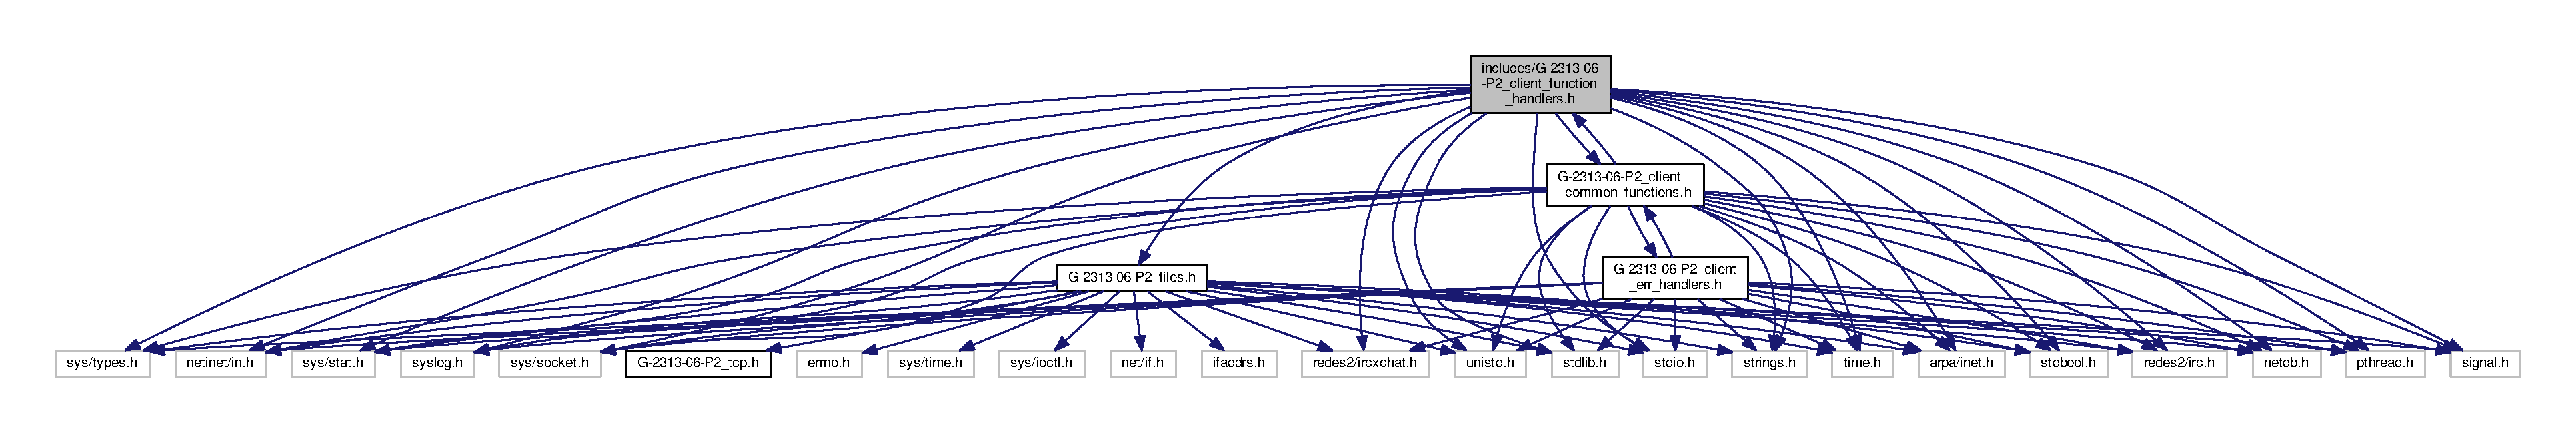
\includegraphics[width=350pt]{G-2313-06-P2__client__function__handlers_8h__incl}
\end{center}
\end{figure}
Gráfico de los archivos que directa o indirectamente incluyen a este archivo\+:\nopagebreak
\begin{figure}[H]
\begin{center}
\leavevmode
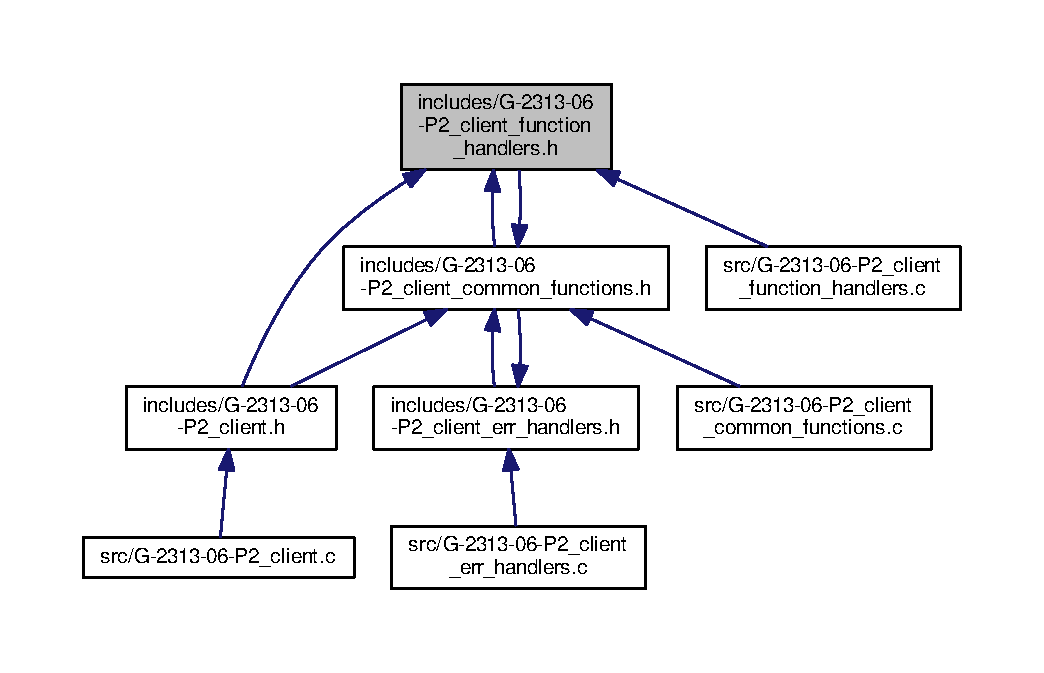
\includegraphics[width=350pt]{G-2313-06-P2__client__function__handlers_8h__dep__incl}
\end{center}
\end{figure}
\subsection*{Funciones}
\begin{DoxyCompactItemize}
\item 
void \hyperlink{G-2313-06-P2__client__function__handlers_8h_a3271de16b2f7077059343bd6f52e4866}{server\+\_\+in\+\_\+command\+\_\+nick} (char $\ast$command)
\item 
void \hyperlink{G-2313-06-P2__client__function__handlers_8h_a64c324e32edf01774722861d3abc7be3}{server\+\_\+in\+\_\+command\+\_\+join} (char $\ast$command)
\item 
void \hyperlink{G-2313-06-P2__client__function__handlers_8h_a53568ffb9d2301140815861c2f7178ad}{server\+\_\+in\+\_\+command\+\_\+part} (char $\ast$command)
\item 
void \hyperlink{G-2313-06-P2__client__function__handlers_8h_ae5f66619469f8ea0efa0a7a5d75938dc}{server\+\_\+in\+\_\+command\+\_\+mode} (char $\ast$command)
\item 
void \hyperlink{G-2313-06-P2__client__function__handlers_8h_ad908abfd32d53b9483d5afa4ca18ff14}{server\+\_\+in\+\_\+command\+\_\+topic} (char $\ast$command)
\item 
void \hyperlink{G-2313-06-P2__client__function__handlers_8h_aa3d18c616914957b9794f086466788bb}{server\+\_\+in\+\_\+command\+\_\+kick} (char $\ast$command)
\item 
void \hyperlink{G-2313-06-P2__client__function__handlers_8h_a858c0e5586286e535590f7de14620300}{server\+\_\+in\+\_\+command\+\_\+who} (char $\ast$command)
\item 
void \hyperlink{G-2313-06-P2__client__function__handlers_8h_a32594eebe5482f63993568825a9e126a}{server\+\_\+in\+\_\+command\+\_\+privmsg} (char $\ast$command)
\item 
void \hyperlink{G-2313-06-P2__client__function__handlers_8h_a09a9d4d13037bd783036a70d5a76ac46}{server\+\_\+in\+\_\+command\+\_\+ping} (char $\ast$command)
\item 
void \hyperlink{G-2313-06-P2__client__function__handlers_8h_a06042a6459e89e0ae7586e66f8595fa3}{server\+\_\+in\+\_\+command\+\_\+pong} (char $\ast$command)
\item 
void \hyperlink{G-2313-06-P2__client__function__handlers_8h_a294ef5e5070e9859d88beb603ef950f2}{server\+\_\+in\+\_\+command\+\_\+rpl\+\_\+welcome} (char $\ast$command)
\item 
void \hyperlink{G-2313-06-P2__client__function__handlers_8h_a40e46db4017fb76fc547536d9c51f5d9}{server\+\_\+in\+\_\+command\+\_\+rpl\+\_\+created} (char $\ast$command)
\item 
void \hyperlink{G-2313-06-P2__client__function__handlers_8h_a3f4cf6c0d74b06a0916f7a9619972eee}{server\+\_\+in\+\_\+command\+\_\+rpl\+\_\+yourhost} (char $\ast$command)
\item 
void \hyperlink{G-2313-06-P2__client__function__handlers_8h_af5091cf59cbab7ce259c405c019fa8dd}{server\+\_\+in\+\_\+command\+\_\+rpl\+\_\+luserclient} (char $\ast$command)
\item 
void \hyperlink{G-2313-06-P2__client__function__handlers_8h_a5764225aa28906c7ccebf0996b2c5a08}{server\+\_\+in\+\_\+command\+\_\+rpl\+\_\+luserme} (char $\ast$command)
\item 
void \hyperlink{G-2313-06-P2__client__function__handlers_8h_acd688f18855dcb6ee9bf10a72e0c8f6c}{server\+\_\+in\+\_\+command\+\_\+rpl\+\_\+motdstart} (char $\ast$command)
\item 
void \hyperlink{G-2313-06-P2__client__function__handlers_8h_a774c98f4ea94eb6f92a5b22d33030674}{server\+\_\+in\+\_\+command\+\_\+rpl\+\_\+motd} (char $\ast$command)
\item 
void \hyperlink{G-2313-06-P2__client__function__handlers_8h_ad22233e08c30cad9e0598f80b5b38744}{server\+\_\+in\+\_\+command\+\_\+rpl\+\_\+endofmotd} (char $\ast$command)
\item 
void \hyperlink{G-2313-06-P2__client__function__handlers_8h_a86782df5d9b151dd061b9831a47a2c5f}{server\+\_\+in\+\_\+command\+\_\+rpl\+\_\+whoreply} (char $\ast$command)
\item 
void \hyperlink{G-2313-06-P2__client__function__handlers_8h_add282510a7e92a90d45091e6dc3a3488}{server\+\_\+in\+\_\+command\+\_\+rpl\+\_\+away} (char $\ast$command)
\item 
void \hyperlink{G-2313-06-P2__client__function__handlers_8h_ada377e1754f9a22a2ebe0bada8838b5b}{server\+\_\+in\+\_\+command\+\_\+rpl\+\_\+nowaway} (char $\ast$command)
\item 
void \hyperlink{G-2313-06-P2__client__function__handlers_8h_abc030e3bc9ce4ad126ea2c66e304e2d5}{server\+\_\+in\+\_\+command\+\_\+rpl\+\_\+topic} (char $\ast$command)
\item 
void \hyperlink{G-2313-06-P2__client__function__handlers_8h_ab9b55bd1e18bde61e8327fcf6936d91f}{server\+\_\+in\+\_\+command\+\_\+rpl\+\_\+notopic} (char $\ast$command)
\item 
void \hyperlink{G-2313-06-P2__client__function__handlers_8h_a24bb76a5941798964a8dd18e1cfb1d81}{server\+\_\+in\+\_\+command\+\_\+rpl\+\_\+youroper} (char $\ast$command)
\item 
void \hyperlink{G-2313-06-P2__client__function__handlers_8h_aa885b5d729d8a920a1c38678abdbe6b7}{server\+\_\+in\+\_\+command\+\_\+rpl\+\_\+luserop} (char $\ast$command)
\item 
void \hyperlink{G-2313-06-P2__client__function__handlers_8h_ae53c29cff5b1b8b3981be92c317cf29d}{server\+\_\+in\+\_\+command\+\_\+rpl\+\_\+luserchannels} (char $\ast$command)
\item 
void \hyperlink{G-2313-06-P2__client__function__handlers_8h_a9a54a1989e86596904bc4d1c2618ba84}{server\+\_\+in\+\_\+command\+\_\+rpl\+\_\+youreservice} (char $\ast$command)
\item 
void \hyperlink{G-2313-06-P2__client__function__handlers_8h_aa4c4d377b1cde9f0b40997a54c81c3de}{server\+\_\+in\+\_\+command\+\_\+rpl\+\_\+myinfo} (char $\ast$command)
\item 
void \hyperlink{G-2313-06-P2__client__function__handlers_8h_a441993de1d4be974fab21e17aacc553e}{server\+\_\+in\+\_\+command\+\_\+rpl\+\_\+endofwho} (char $\ast$command)
\item 
void \hyperlink{G-2313-06-P2__client__function__handlers_8h_a56185c77cfea8620c1ce413a44865bc4}{server\+\_\+in\+\_\+command\+\_\+rpl\+\_\+endofwhois} (char $\ast$command)
\item 
void \hyperlink{G-2313-06-P2__client__function__handlers_8h_a6477df39f199931be3274e311a18b276}{server\+\_\+in\+\_\+command\+\_\+rpl\+\_\+info} (char $\ast$command)
\item 
void \hyperlink{G-2313-06-P2__client__function__handlers_8h_af2190c9ca68abe019cde6f3a18e380c2}{server\+\_\+in\+\_\+command\+\_\+rpl\+\_\+whoisuser} (char $\ast$command)
\item 
void \hyperlink{G-2313-06-P2__client__function__handlers_8h_a7ed4d1bd7f485fe7c6d26bd1d8eef662}{server\+\_\+in\+\_\+command\+\_\+rpl\+\_\+whoischannels} (char $\ast$command)
\item 
void \hyperlink{G-2313-06-P2__client__function__handlers_8h_a890fb67530ca5c1f5c14da877fc9ba21}{server\+\_\+in\+\_\+command\+\_\+rpl\+\_\+whoisoperator} (char $\ast$command)
\item 
void \hyperlink{G-2313-06-P2__client__function__handlers_8h_a27bc970f66b7e5a2f3806853c3fa156f}{server\+\_\+in\+\_\+command\+\_\+rpl\+\_\+whoisserver} (char $\ast$command)
\item 
void \hyperlink{G-2313-06-P2__client__function__handlers_8h_ada14de5a081899ca2b5eccbfb9779d62}{server\+\_\+in\+\_\+command\+\_\+rpl\+\_\+whoisidle} (char $\ast$command)
\item 
void \hyperlink{G-2313-06-P2__client__function__handlers_8h_a23ae57a558e401f83bc03209efb34be2}{server\+\_\+in\+\_\+command\+\_\+rpl\+\_\+channelmodeis} (char $\ast$command)
\item 
void \hyperlink{G-2313-06-P2__client__function__handlers_8h_a11fdd753a098bb69dc7ca93a89433abb}{server\+\_\+in\+\_\+command\+\_\+rpl\+\_\+endofnames} (char $\ast$command)
\item 
void \hyperlink{G-2313-06-P2__client__function__handlers_8h_a032cc47903f14a4fbdcec9e54f6a8e4a}{server\+\_\+in\+\_\+command\+\_\+rpl\+\_\+list} (char $\ast$command)
\item 
void \hyperlink{G-2313-06-P2__client__function__handlers_8h_ad4a1e3d492ae6907a5e15e92cb9b69f7}{server\+\_\+in\+\_\+command\+\_\+rpl\+\_\+listend} (char $\ast$command)
\item 
void \hyperlink{G-2313-06-P2__client__function__handlers_8h_a770ed57ba6c48c4a349208439e3f19ef}{server\+\_\+in\+\_\+command\+\_\+rpl\+\_\+namreply} (char $\ast$command)
\item 
void \hyperlink{G-2313-06-P2__client__function__handlers_8h_a43f3e63fcf23bd087e02911f79b789b0}{server\+\_\+out\+\_\+command\+\_\+nick} (char $\ast$command)
\item 
void \hyperlink{G-2313-06-P2__client__function__handlers_8h_a49e60d29aef3725ab2a91c7f99e61021}{server\+\_\+out\+\_\+command\+\_\+join} (char $\ast$command)
\item 
void \hyperlink{G-2313-06-P2__client__function__handlers_8h_ab2f3bd779063c27074a6cdce0f98ee0a}{server\+\_\+out\+\_\+command\+\_\+names} (char $\ast$command)
\item 
void \hyperlink{G-2313-06-P2__client__function__handlers_8h_a0a66dad6908cd303ae31f06dda298e5f}{server\+\_\+out\+\_\+command\+\_\+list} (char $\ast$command)
\item 
void \hyperlink{G-2313-06-P2__client__function__handlers_8h_a39f81214b8394e2b7fb0989e5fe10fb3}{server\+\_\+out\+\_\+command\+\_\+part} (char $\ast$command)
\item 
void \hyperlink{G-2313-06-P2__client__function__handlers_8h_afa583197101ff2eb07ab93ccd10da962}{server\+\_\+out\+\_\+command\+\_\+mode} (char $\ast$command)
\item 
void \hyperlink{G-2313-06-P2__client__function__handlers_8h_a4e94d9864089e10109fc24ce92d4368b}{server\+\_\+out\+\_\+command\+\_\+kick} (char $\ast$command)
\item 
void \hyperlink{G-2313-06-P2__client__function__handlers_8h_a4c442d20949a3a3e84551a5f23ce8263}{server\+\_\+out\+\_\+command\+\_\+privmsg} (char $\ast$command)
\item 
void \hyperlink{G-2313-06-P2__client__function__handlers_8h_af34c02fb3b13802e2c457a302c66cb89}{server\+\_\+out\+\_\+command\+\_\+whois} (char $\ast$command)
\item 
void \hyperlink{G-2313-06-P2__client__function__handlers_8h_a6760491bb5560bf6db1e652022f0720f}{server\+\_\+out\+\_\+command\+\_\+invite} (char $\ast$command)
\item 
void \hyperlink{G-2313-06-P2__client__function__handlers_8h_affd97f456e87778153ec551468bb7f25}{server\+\_\+out\+\_\+command\+\_\+topic} (char $\ast$command)
\item 
void \hyperlink{G-2313-06-P2__client__function__handlers_8h_a9680c711ecaa492727c14a9c5d7e82ca}{server\+\_\+out\+\_\+command\+\_\+me} (char $\ast$command)
\item 
void \hyperlink{G-2313-06-P2__client__function__handlers_8h_ad2280719361affeaf8d3a663b48f0b3f}{server\+\_\+out\+\_\+command\+\_\+msg} (char $\ast$command)
\item 
void \hyperlink{G-2313-06-P2__client__function__handlers_8h_a6e05dad9592e0e473e84647cfe263034}{server\+\_\+out\+\_\+command\+\_\+notice} (char $\ast$command)
\item 
void \hyperlink{G-2313-06-P2__client__function__handlers_8h_a3b0bef634e60a6e59223cfb7e444fb36}{server\+\_\+out\+\_\+command\+\_\+ignore} (char $\ast$command)
\item 
void \hyperlink{G-2313-06-P2__client__function__handlers_8h_a4f8f2db21b7edd9e6b7fbad232ee27fd}{server\+\_\+out\+\_\+command\+\_\+who} (char $\ast$command)
\item 
void \hyperlink{G-2313-06-P2__client__function__handlers_8h_a74f475c007446256a2cbada71f51f30a}{server\+\_\+out\+\_\+command\+\_\+whowas} (char $\ast$command)
\item 
void \hyperlink{G-2313-06-P2__client__function__handlers_8h_ae721ae6a65ec5f0790d6b6883dcf94a5}{server\+\_\+out\+\_\+command\+\_\+motd} (char $\ast$command)
\item 
void \hyperlink{G-2313-06-P2__client__function__handlers_8h_ac0c8a1e0d4144fd3d78c124bad9228d6}{server\+\_\+out\+\_\+command\+\_\+away} (char $\ast$command)
\item 
void \hyperlink{G-2313-06-P2__client__function__handlers_8h_a3719651e6671245a46f4994fcf462c7d}{server\+\_\+out\+\_\+command\+\_\+ping} (char $\ast$command)
\end{DoxyCompactItemize}


\subsection{Documentación de las funciones}
\index{G-\/2313-\/06-\/\+P2\+\_\+client\+\_\+function\+\_\+handlers.\+h@{G-\/2313-\/06-\/\+P2\+\_\+client\+\_\+function\+\_\+handlers.\+h}!server\+\_\+in\+\_\+command\+\_\+join@{server\+\_\+in\+\_\+command\+\_\+join}}
\index{server\+\_\+in\+\_\+command\+\_\+join@{server\+\_\+in\+\_\+command\+\_\+join}!G-\/2313-\/06-\/\+P2\+\_\+client\+\_\+function\+\_\+handlers.\+h@{G-\/2313-\/06-\/\+P2\+\_\+client\+\_\+function\+\_\+handlers.\+h}}
\subsubsection[{\texorpdfstring{server\+\_\+in\+\_\+command\+\_\+join(char $\ast$command)}{server_in_command_join(char *command)}}]{\setlength{\rightskip}{0pt plus 5cm}void server\+\_\+in\+\_\+command\+\_\+join (
\begin{DoxyParamCaption}
\item[{char $\ast$}]{command}
\end{DoxyParamCaption}
)}\hypertarget{G-2313-06-P2__client__function__handlers_8h_a64c324e32edf01774722861d3abc7be3}{}\label{G-2313-06-P2__client__function__handlers_8h_a64c324e32edf01774722861d3abc7be3}


Definición en la línea 51 del archivo G-\/2313-\/06-\/\+P2\+\_\+client\+\_\+function\+\_\+handlers.\+c.

\index{G-\/2313-\/06-\/\+P2\+\_\+client\+\_\+function\+\_\+handlers.\+h@{G-\/2313-\/06-\/\+P2\+\_\+client\+\_\+function\+\_\+handlers.\+h}!server\+\_\+in\+\_\+command\+\_\+kick@{server\+\_\+in\+\_\+command\+\_\+kick}}
\index{server\+\_\+in\+\_\+command\+\_\+kick@{server\+\_\+in\+\_\+command\+\_\+kick}!G-\/2313-\/06-\/\+P2\+\_\+client\+\_\+function\+\_\+handlers.\+h@{G-\/2313-\/06-\/\+P2\+\_\+client\+\_\+function\+\_\+handlers.\+h}}
\subsubsection[{\texorpdfstring{server\+\_\+in\+\_\+command\+\_\+kick(char $\ast$command)}{server_in_command_kick(char *command)}}]{\setlength{\rightskip}{0pt plus 5cm}void server\+\_\+in\+\_\+command\+\_\+kick (
\begin{DoxyParamCaption}
\item[{char $\ast$}]{command}
\end{DoxyParamCaption}
)}\hypertarget{G-2313-06-P2__client__function__handlers_8h_aa3d18c616914957b9794f086466788bb}{}\label{G-2313-06-P2__client__function__handlers_8h_aa3d18c616914957b9794f086466788bb}


Definición en la línea 204 del archivo G-\/2313-\/06-\/\+P2\+\_\+client\+\_\+function\+\_\+handlers.\+c.

\index{G-\/2313-\/06-\/\+P2\+\_\+client\+\_\+function\+\_\+handlers.\+h@{G-\/2313-\/06-\/\+P2\+\_\+client\+\_\+function\+\_\+handlers.\+h}!server\+\_\+in\+\_\+command\+\_\+mode@{server\+\_\+in\+\_\+command\+\_\+mode}}
\index{server\+\_\+in\+\_\+command\+\_\+mode@{server\+\_\+in\+\_\+command\+\_\+mode}!G-\/2313-\/06-\/\+P2\+\_\+client\+\_\+function\+\_\+handlers.\+h@{G-\/2313-\/06-\/\+P2\+\_\+client\+\_\+function\+\_\+handlers.\+h}}
\subsubsection[{\texorpdfstring{server\+\_\+in\+\_\+command\+\_\+mode(char $\ast$command)}{server_in_command_mode(char *command)}}]{\setlength{\rightskip}{0pt plus 5cm}void server\+\_\+in\+\_\+command\+\_\+mode (
\begin{DoxyParamCaption}
\item[{char $\ast$}]{command}
\end{DoxyParamCaption}
)}\hypertarget{G-2313-06-P2__client__function__handlers_8h_ae5f66619469f8ea0efa0a7a5d75938dc}{}\label{G-2313-06-P2__client__function__handlers_8h_ae5f66619469f8ea0efa0a7a5d75938dc}


Definición en la línea 103 del archivo G-\/2313-\/06-\/\+P2\+\_\+client\+\_\+function\+\_\+handlers.\+c.

\index{G-\/2313-\/06-\/\+P2\+\_\+client\+\_\+function\+\_\+handlers.\+h@{G-\/2313-\/06-\/\+P2\+\_\+client\+\_\+function\+\_\+handlers.\+h}!server\+\_\+in\+\_\+command\+\_\+nick@{server\+\_\+in\+\_\+command\+\_\+nick}}
\index{server\+\_\+in\+\_\+command\+\_\+nick@{server\+\_\+in\+\_\+command\+\_\+nick}!G-\/2313-\/06-\/\+P2\+\_\+client\+\_\+function\+\_\+handlers.\+h@{G-\/2313-\/06-\/\+P2\+\_\+client\+\_\+function\+\_\+handlers.\+h}}
\subsubsection[{\texorpdfstring{server\+\_\+in\+\_\+command\+\_\+nick(char $\ast$command)}{server_in_command_nick(char *command)}}]{\setlength{\rightskip}{0pt plus 5cm}void server\+\_\+in\+\_\+command\+\_\+nick (
\begin{DoxyParamCaption}
\item[{char $\ast$}]{command}
\end{DoxyParamCaption}
)}\hypertarget{G-2313-06-P2__client__function__handlers_8h_a3271de16b2f7077059343bd6f52e4866}{}\label{G-2313-06-P2__client__function__handlers_8h_a3271de16b2f7077059343bd6f52e4866}


Definición en la línea 7 del archivo G-\/2313-\/06-\/\+P2\+\_\+client\+\_\+function\+\_\+handlers.\+c.

\index{G-\/2313-\/06-\/\+P2\+\_\+client\+\_\+function\+\_\+handlers.\+h@{G-\/2313-\/06-\/\+P2\+\_\+client\+\_\+function\+\_\+handlers.\+h}!server\+\_\+in\+\_\+command\+\_\+part@{server\+\_\+in\+\_\+command\+\_\+part}}
\index{server\+\_\+in\+\_\+command\+\_\+part@{server\+\_\+in\+\_\+command\+\_\+part}!G-\/2313-\/06-\/\+P2\+\_\+client\+\_\+function\+\_\+handlers.\+h@{G-\/2313-\/06-\/\+P2\+\_\+client\+\_\+function\+\_\+handlers.\+h}}
\subsubsection[{\texorpdfstring{server\+\_\+in\+\_\+command\+\_\+part(char $\ast$command)}{server_in_command_part(char *command)}}]{\setlength{\rightskip}{0pt plus 5cm}void server\+\_\+in\+\_\+command\+\_\+part (
\begin{DoxyParamCaption}
\item[{char $\ast$}]{command}
\end{DoxyParamCaption}
)}\hypertarget{G-2313-06-P2__client__function__handlers_8h_a53568ffb9d2301140815861c2f7178ad}{}\label{G-2313-06-P2__client__function__handlers_8h_a53568ffb9d2301140815861c2f7178ad}


Definición en la línea 83 del archivo G-\/2313-\/06-\/\+P2\+\_\+client\+\_\+function\+\_\+handlers.\+c.

\index{G-\/2313-\/06-\/\+P2\+\_\+client\+\_\+function\+\_\+handlers.\+h@{G-\/2313-\/06-\/\+P2\+\_\+client\+\_\+function\+\_\+handlers.\+h}!server\+\_\+in\+\_\+command\+\_\+ping@{server\+\_\+in\+\_\+command\+\_\+ping}}
\index{server\+\_\+in\+\_\+command\+\_\+ping@{server\+\_\+in\+\_\+command\+\_\+ping}!G-\/2313-\/06-\/\+P2\+\_\+client\+\_\+function\+\_\+handlers.\+h@{G-\/2313-\/06-\/\+P2\+\_\+client\+\_\+function\+\_\+handlers.\+h}}
\subsubsection[{\texorpdfstring{server\+\_\+in\+\_\+command\+\_\+ping(char $\ast$command)}{server_in_command_ping(char *command)}}]{\setlength{\rightskip}{0pt plus 5cm}void server\+\_\+in\+\_\+command\+\_\+ping (
\begin{DoxyParamCaption}
\item[{char $\ast$}]{command}
\end{DoxyParamCaption}
)}\hypertarget{G-2313-06-P2__client__function__handlers_8h_a09a9d4d13037bd783036a70d5a76ac46}{}\label{G-2313-06-P2__client__function__handlers_8h_a09a9d4d13037bd783036a70d5a76ac46}


Definición en la línea 274 del archivo G-\/2313-\/06-\/\+P2\+\_\+client\+\_\+function\+\_\+handlers.\+c.

\index{G-\/2313-\/06-\/\+P2\+\_\+client\+\_\+function\+\_\+handlers.\+h@{G-\/2313-\/06-\/\+P2\+\_\+client\+\_\+function\+\_\+handlers.\+h}!server\+\_\+in\+\_\+command\+\_\+pong@{server\+\_\+in\+\_\+command\+\_\+pong}}
\index{server\+\_\+in\+\_\+command\+\_\+pong@{server\+\_\+in\+\_\+command\+\_\+pong}!G-\/2313-\/06-\/\+P2\+\_\+client\+\_\+function\+\_\+handlers.\+h@{G-\/2313-\/06-\/\+P2\+\_\+client\+\_\+function\+\_\+handlers.\+h}}
\subsubsection[{\texorpdfstring{server\+\_\+in\+\_\+command\+\_\+pong(char $\ast$command)}{server_in_command_pong(char *command)}}]{\setlength{\rightskip}{0pt plus 5cm}void server\+\_\+in\+\_\+command\+\_\+pong (
\begin{DoxyParamCaption}
\item[{char $\ast$}]{command}
\end{DoxyParamCaption}
)}\hypertarget{G-2313-06-P2__client__function__handlers_8h_a06042a6459e89e0ae7586e66f8595fa3}{}\label{G-2313-06-P2__client__function__handlers_8h_a06042a6459e89e0ae7586e66f8595fa3}


Definición en la línea 289 del archivo G-\/2313-\/06-\/\+P2\+\_\+client\+\_\+function\+\_\+handlers.\+c.

\index{G-\/2313-\/06-\/\+P2\+\_\+client\+\_\+function\+\_\+handlers.\+h@{G-\/2313-\/06-\/\+P2\+\_\+client\+\_\+function\+\_\+handlers.\+h}!server\+\_\+in\+\_\+command\+\_\+privmsg@{server\+\_\+in\+\_\+command\+\_\+privmsg}}
\index{server\+\_\+in\+\_\+command\+\_\+privmsg@{server\+\_\+in\+\_\+command\+\_\+privmsg}!G-\/2313-\/06-\/\+P2\+\_\+client\+\_\+function\+\_\+handlers.\+h@{G-\/2313-\/06-\/\+P2\+\_\+client\+\_\+function\+\_\+handlers.\+h}}
\subsubsection[{\texorpdfstring{server\+\_\+in\+\_\+command\+\_\+privmsg(char $\ast$command)}{server_in_command_privmsg(char *command)}}]{\setlength{\rightskip}{0pt plus 5cm}void server\+\_\+in\+\_\+command\+\_\+privmsg (
\begin{DoxyParamCaption}
\item[{char $\ast$}]{command}
\end{DoxyParamCaption}
)}\hypertarget{G-2313-06-P2__client__function__handlers_8h_a32594eebe5482f63993568825a9e126a}{}\label{G-2313-06-P2__client__function__handlers_8h_a32594eebe5482f63993568825a9e126a}


Definición en la línea 241 del archivo G-\/2313-\/06-\/\+P2\+\_\+client\+\_\+function\+\_\+handlers.\+c.

\index{G-\/2313-\/06-\/\+P2\+\_\+client\+\_\+function\+\_\+handlers.\+h@{G-\/2313-\/06-\/\+P2\+\_\+client\+\_\+function\+\_\+handlers.\+h}!server\+\_\+in\+\_\+command\+\_\+rpl\+\_\+away@{server\+\_\+in\+\_\+command\+\_\+rpl\+\_\+away}}
\index{server\+\_\+in\+\_\+command\+\_\+rpl\+\_\+away@{server\+\_\+in\+\_\+command\+\_\+rpl\+\_\+away}!G-\/2313-\/06-\/\+P2\+\_\+client\+\_\+function\+\_\+handlers.\+h@{G-\/2313-\/06-\/\+P2\+\_\+client\+\_\+function\+\_\+handlers.\+h}}
\subsubsection[{\texorpdfstring{server\+\_\+in\+\_\+command\+\_\+rpl\+\_\+away(char $\ast$command)}{server_in_command_rpl_away(char *command)}}]{\setlength{\rightskip}{0pt plus 5cm}void server\+\_\+in\+\_\+command\+\_\+rpl\+\_\+away (
\begin{DoxyParamCaption}
\item[{char $\ast$}]{command}
\end{DoxyParamCaption}
)}\hypertarget{G-2313-06-P2__client__function__handlers_8h_add282510a7e92a90d45091e6dc3a3488}{}\label{G-2313-06-P2__client__function__handlers_8h_add282510a7e92a90d45091e6dc3a3488}


Definición en la línea 407 del archivo G-\/2313-\/06-\/\+P2\+\_\+client\+\_\+function\+\_\+handlers.\+c.

\index{G-\/2313-\/06-\/\+P2\+\_\+client\+\_\+function\+\_\+handlers.\+h@{G-\/2313-\/06-\/\+P2\+\_\+client\+\_\+function\+\_\+handlers.\+h}!server\+\_\+in\+\_\+command\+\_\+rpl\+\_\+channelmodeis@{server\+\_\+in\+\_\+command\+\_\+rpl\+\_\+channelmodeis}}
\index{server\+\_\+in\+\_\+command\+\_\+rpl\+\_\+channelmodeis@{server\+\_\+in\+\_\+command\+\_\+rpl\+\_\+channelmodeis}!G-\/2313-\/06-\/\+P2\+\_\+client\+\_\+function\+\_\+handlers.\+h@{G-\/2313-\/06-\/\+P2\+\_\+client\+\_\+function\+\_\+handlers.\+h}}
\subsubsection[{\texorpdfstring{server\+\_\+in\+\_\+command\+\_\+rpl\+\_\+channelmodeis(char $\ast$command)}{server_in_command_rpl_channelmodeis(char *command)}}]{\setlength{\rightskip}{0pt plus 5cm}void server\+\_\+in\+\_\+command\+\_\+rpl\+\_\+channelmodeis (
\begin{DoxyParamCaption}
\item[{char $\ast$}]{command}
\end{DoxyParamCaption}
)}\hypertarget{G-2313-06-P2__client__function__handlers_8h_a23ae57a558e401f83bc03209efb34be2}{}\label{G-2313-06-P2__client__function__handlers_8h_a23ae57a558e401f83bc03209efb34be2}


Definición en la línea 599 del archivo G-\/2313-\/06-\/\+P2\+\_\+client\+\_\+function\+\_\+handlers.\+c.

\index{G-\/2313-\/06-\/\+P2\+\_\+client\+\_\+function\+\_\+handlers.\+h@{G-\/2313-\/06-\/\+P2\+\_\+client\+\_\+function\+\_\+handlers.\+h}!server\+\_\+in\+\_\+command\+\_\+rpl\+\_\+created@{server\+\_\+in\+\_\+command\+\_\+rpl\+\_\+created}}
\index{server\+\_\+in\+\_\+command\+\_\+rpl\+\_\+created@{server\+\_\+in\+\_\+command\+\_\+rpl\+\_\+created}!G-\/2313-\/06-\/\+P2\+\_\+client\+\_\+function\+\_\+handlers.\+h@{G-\/2313-\/06-\/\+P2\+\_\+client\+\_\+function\+\_\+handlers.\+h}}
\subsubsection[{\texorpdfstring{server\+\_\+in\+\_\+command\+\_\+rpl\+\_\+created(char $\ast$command)}{server_in_command_rpl_created(char *command)}}]{\setlength{\rightskip}{0pt plus 5cm}void server\+\_\+in\+\_\+command\+\_\+rpl\+\_\+created (
\begin{DoxyParamCaption}
\item[{char $\ast$}]{command}
\end{DoxyParamCaption}
)}\hypertarget{G-2313-06-P2__client__function__handlers_8h_a40e46db4017fb76fc547536d9c51f5d9}{}\label{G-2313-06-P2__client__function__handlers_8h_a40e46db4017fb76fc547536d9c51f5d9}


Definición en la línea 318 del archivo G-\/2313-\/06-\/\+P2\+\_\+client\+\_\+function\+\_\+handlers.\+c.

\index{G-\/2313-\/06-\/\+P2\+\_\+client\+\_\+function\+\_\+handlers.\+h@{G-\/2313-\/06-\/\+P2\+\_\+client\+\_\+function\+\_\+handlers.\+h}!server\+\_\+in\+\_\+command\+\_\+rpl\+\_\+endofmotd@{server\+\_\+in\+\_\+command\+\_\+rpl\+\_\+endofmotd}}
\index{server\+\_\+in\+\_\+command\+\_\+rpl\+\_\+endofmotd@{server\+\_\+in\+\_\+command\+\_\+rpl\+\_\+endofmotd}!G-\/2313-\/06-\/\+P2\+\_\+client\+\_\+function\+\_\+handlers.\+h@{G-\/2313-\/06-\/\+P2\+\_\+client\+\_\+function\+\_\+handlers.\+h}}
\subsubsection[{\texorpdfstring{server\+\_\+in\+\_\+command\+\_\+rpl\+\_\+endofmotd(char $\ast$command)}{server_in_command_rpl_endofmotd(char *command)}}]{\setlength{\rightskip}{0pt plus 5cm}void server\+\_\+in\+\_\+command\+\_\+rpl\+\_\+endofmotd (
\begin{DoxyParamCaption}
\item[{char $\ast$}]{command}
\end{DoxyParamCaption}
)}\hypertarget{G-2313-06-P2__client__function__handlers_8h_ad22233e08c30cad9e0598f80b5b38744}{}\label{G-2313-06-P2__client__function__handlers_8h_ad22233e08c30cad9e0598f80b5b38744}


Definición en la línea 374 del archivo G-\/2313-\/06-\/\+P2\+\_\+client\+\_\+function\+\_\+handlers.\+c.

\index{G-\/2313-\/06-\/\+P2\+\_\+client\+\_\+function\+\_\+handlers.\+h@{G-\/2313-\/06-\/\+P2\+\_\+client\+\_\+function\+\_\+handlers.\+h}!server\+\_\+in\+\_\+command\+\_\+rpl\+\_\+endofnames@{server\+\_\+in\+\_\+command\+\_\+rpl\+\_\+endofnames}}
\index{server\+\_\+in\+\_\+command\+\_\+rpl\+\_\+endofnames@{server\+\_\+in\+\_\+command\+\_\+rpl\+\_\+endofnames}!G-\/2313-\/06-\/\+P2\+\_\+client\+\_\+function\+\_\+handlers.\+h@{G-\/2313-\/06-\/\+P2\+\_\+client\+\_\+function\+\_\+handlers.\+h}}
\subsubsection[{\texorpdfstring{server\+\_\+in\+\_\+command\+\_\+rpl\+\_\+endofnames(char $\ast$command)}{server_in_command_rpl_endofnames(char *command)}}]{\setlength{\rightskip}{0pt plus 5cm}void server\+\_\+in\+\_\+command\+\_\+rpl\+\_\+endofnames (
\begin{DoxyParamCaption}
\item[{char $\ast$}]{command}
\end{DoxyParamCaption}
)}\hypertarget{G-2313-06-P2__client__function__handlers_8h_a11fdd753a098bb69dc7ca93a89433abb}{}\label{G-2313-06-P2__client__function__handlers_8h_a11fdd753a098bb69dc7ca93a89433abb}


Definición en la línea 610 del archivo G-\/2313-\/06-\/\+P2\+\_\+client\+\_\+function\+\_\+handlers.\+c.

\index{G-\/2313-\/06-\/\+P2\+\_\+client\+\_\+function\+\_\+handlers.\+h@{G-\/2313-\/06-\/\+P2\+\_\+client\+\_\+function\+\_\+handlers.\+h}!server\+\_\+in\+\_\+command\+\_\+rpl\+\_\+endofwho@{server\+\_\+in\+\_\+command\+\_\+rpl\+\_\+endofwho}}
\index{server\+\_\+in\+\_\+command\+\_\+rpl\+\_\+endofwho@{server\+\_\+in\+\_\+command\+\_\+rpl\+\_\+endofwho}!G-\/2313-\/06-\/\+P2\+\_\+client\+\_\+function\+\_\+handlers.\+h@{G-\/2313-\/06-\/\+P2\+\_\+client\+\_\+function\+\_\+handlers.\+h}}
\subsubsection[{\texorpdfstring{server\+\_\+in\+\_\+command\+\_\+rpl\+\_\+endofwho(char $\ast$command)}{server_in_command_rpl_endofwho(char *command)}}]{\setlength{\rightskip}{0pt plus 5cm}void server\+\_\+in\+\_\+command\+\_\+rpl\+\_\+endofwho (
\begin{DoxyParamCaption}
\item[{char $\ast$}]{command}
\end{DoxyParamCaption}
)}\hypertarget{G-2313-06-P2__client__function__handlers_8h_a441993de1d4be974fab21e17aacc553e}{}\label{G-2313-06-P2__client__function__handlers_8h_a441993de1d4be974fab21e17aacc553e}


Definición en la línea 512 del archivo G-\/2313-\/06-\/\+P2\+\_\+client\+\_\+function\+\_\+handlers.\+c.

\index{G-\/2313-\/06-\/\+P2\+\_\+client\+\_\+function\+\_\+handlers.\+h@{G-\/2313-\/06-\/\+P2\+\_\+client\+\_\+function\+\_\+handlers.\+h}!server\+\_\+in\+\_\+command\+\_\+rpl\+\_\+endofwhois@{server\+\_\+in\+\_\+command\+\_\+rpl\+\_\+endofwhois}}
\index{server\+\_\+in\+\_\+command\+\_\+rpl\+\_\+endofwhois@{server\+\_\+in\+\_\+command\+\_\+rpl\+\_\+endofwhois}!G-\/2313-\/06-\/\+P2\+\_\+client\+\_\+function\+\_\+handlers.\+h@{G-\/2313-\/06-\/\+P2\+\_\+client\+\_\+function\+\_\+handlers.\+h}}
\subsubsection[{\texorpdfstring{server\+\_\+in\+\_\+command\+\_\+rpl\+\_\+endofwhois(char $\ast$command)}{server_in_command_rpl_endofwhois(char *command)}}]{\setlength{\rightskip}{0pt plus 5cm}void server\+\_\+in\+\_\+command\+\_\+rpl\+\_\+endofwhois (
\begin{DoxyParamCaption}
\item[{char $\ast$}]{command}
\end{DoxyParamCaption}
)}\hypertarget{G-2313-06-P2__client__function__handlers_8h_a56185c77cfea8620c1ce413a44865bc4}{}\label{G-2313-06-P2__client__function__handlers_8h_a56185c77cfea8620c1ce413a44865bc4}


Definición en la línea 521 del archivo G-\/2313-\/06-\/\+P2\+\_\+client\+\_\+function\+\_\+handlers.\+c.

\index{G-\/2313-\/06-\/\+P2\+\_\+client\+\_\+function\+\_\+handlers.\+h@{G-\/2313-\/06-\/\+P2\+\_\+client\+\_\+function\+\_\+handlers.\+h}!server\+\_\+in\+\_\+command\+\_\+rpl\+\_\+info@{server\+\_\+in\+\_\+command\+\_\+rpl\+\_\+info}}
\index{server\+\_\+in\+\_\+command\+\_\+rpl\+\_\+info@{server\+\_\+in\+\_\+command\+\_\+rpl\+\_\+info}!G-\/2313-\/06-\/\+P2\+\_\+client\+\_\+function\+\_\+handlers.\+h@{G-\/2313-\/06-\/\+P2\+\_\+client\+\_\+function\+\_\+handlers.\+h}}
\subsubsection[{\texorpdfstring{server\+\_\+in\+\_\+command\+\_\+rpl\+\_\+info(char $\ast$command)}{server_in_command_rpl_info(char *command)}}]{\setlength{\rightskip}{0pt plus 5cm}void server\+\_\+in\+\_\+command\+\_\+rpl\+\_\+info (
\begin{DoxyParamCaption}
\item[{char $\ast$}]{command}
\end{DoxyParamCaption}
)}\hypertarget{G-2313-06-P2__client__function__handlers_8h_a6477df39f199931be3274e311a18b276}{}\label{G-2313-06-P2__client__function__handlers_8h_a6477df39f199931be3274e311a18b276}


Definición en la línea 530 del archivo G-\/2313-\/06-\/\+P2\+\_\+client\+\_\+function\+\_\+handlers.\+c.

\index{G-\/2313-\/06-\/\+P2\+\_\+client\+\_\+function\+\_\+handlers.\+h@{G-\/2313-\/06-\/\+P2\+\_\+client\+\_\+function\+\_\+handlers.\+h}!server\+\_\+in\+\_\+command\+\_\+rpl\+\_\+list@{server\+\_\+in\+\_\+command\+\_\+rpl\+\_\+list}}
\index{server\+\_\+in\+\_\+command\+\_\+rpl\+\_\+list@{server\+\_\+in\+\_\+command\+\_\+rpl\+\_\+list}!G-\/2313-\/06-\/\+P2\+\_\+client\+\_\+function\+\_\+handlers.\+h@{G-\/2313-\/06-\/\+P2\+\_\+client\+\_\+function\+\_\+handlers.\+h}}
\subsubsection[{\texorpdfstring{server\+\_\+in\+\_\+command\+\_\+rpl\+\_\+list(char $\ast$command)}{server_in_command_rpl_list(char *command)}}]{\setlength{\rightskip}{0pt plus 5cm}void server\+\_\+in\+\_\+command\+\_\+rpl\+\_\+list (
\begin{DoxyParamCaption}
\item[{char $\ast$}]{command}
\end{DoxyParamCaption}
)}\hypertarget{G-2313-06-P2__client__function__handlers_8h_a032cc47903f14a4fbdcec9e54f6a8e4a}{}\label{G-2313-06-P2__client__function__handlers_8h_a032cc47903f14a4fbdcec9e54f6a8e4a}


Definición en la línea 619 del archivo G-\/2313-\/06-\/\+P2\+\_\+client\+\_\+function\+\_\+handlers.\+c.

\index{G-\/2313-\/06-\/\+P2\+\_\+client\+\_\+function\+\_\+handlers.\+h@{G-\/2313-\/06-\/\+P2\+\_\+client\+\_\+function\+\_\+handlers.\+h}!server\+\_\+in\+\_\+command\+\_\+rpl\+\_\+listend@{server\+\_\+in\+\_\+command\+\_\+rpl\+\_\+listend}}
\index{server\+\_\+in\+\_\+command\+\_\+rpl\+\_\+listend@{server\+\_\+in\+\_\+command\+\_\+rpl\+\_\+listend}!G-\/2313-\/06-\/\+P2\+\_\+client\+\_\+function\+\_\+handlers.\+h@{G-\/2313-\/06-\/\+P2\+\_\+client\+\_\+function\+\_\+handlers.\+h}}
\subsubsection[{\texorpdfstring{server\+\_\+in\+\_\+command\+\_\+rpl\+\_\+listend(char $\ast$command)}{server_in_command_rpl_listend(char *command)}}]{\setlength{\rightskip}{0pt plus 5cm}void server\+\_\+in\+\_\+command\+\_\+rpl\+\_\+listend (
\begin{DoxyParamCaption}
\item[{char $\ast$}]{command}
\end{DoxyParamCaption}
)}\hypertarget{G-2313-06-P2__client__function__handlers_8h_ad4a1e3d492ae6907a5e15e92cb9b69f7}{}\label{G-2313-06-P2__client__function__handlers_8h_ad4a1e3d492ae6907a5e15e92cb9b69f7}


Definición en la línea 630 del archivo G-\/2313-\/06-\/\+P2\+\_\+client\+\_\+function\+\_\+handlers.\+c.

\index{G-\/2313-\/06-\/\+P2\+\_\+client\+\_\+function\+\_\+handlers.\+h@{G-\/2313-\/06-\/\+P2\+\_\+client\+\_\+function\+\_\+handlers.\+h}!server\+\_\+in\+\_\+command\+\_\+rpl\+\_\+luserchannels@{server\+\_\+in\+\_\+command\+\_\+rpl\+\_\+luserchannels}}
\index{server\+\_\+in\+\_\+command\+\_\+rpl\+\_\+luserchannels@{server\+\_\+in\+\_\+command\+\_\+rpl\+\_\+luserchannels}!G-\/2313-\/06-\/\+P2\+\_\+client\+\_\+function\+\_\+handlers.\+h@{G-\/2313-\/06-\/\+P2\+\_\+client\+\_\+function\+\_\+handlers.\+h}}
\subsubsection[{\texorpdfstring{server\+\_\+in\+\_\+command\+\_\+rpl\+\_\+luserchannels(char $\ast$command)}{server_in_command_rpl_luserchannels(char *command)}}]{\setlength{\rightskip}{0pt plus 5cm}void server\+\_\+in\+\_\+command\+\_\+rpl\+\_\+luserchannels (
\begin{DoxyParamCaption}
\item[{char $\ast$}]{command}
\end{DoxyParamCaption}
)}\hypertarget{G-2313-06-P2__client__function__handlers_8h_ae53c29cff5b1b8b3981be92c317cf29d}{}\label{G-2313-06-P2__client__function__handlers_8h_ae53c29cff5b1b8b3981be92c317cf29d}


Definición en la línea 476 del archivo G-\/2313-\/06-\/\+P2\+\_\+client\+\_\+function\+\_\+handlers.\+c.

\index{G-\/2313-\/06-\/\+P2\+\_\+client\+\_\+function\+\_\+handlers.\+h@{G-\/2313-\/06-\/\+P2\+\_\+client\+\_\+function\+\_\+handlers.\+h}!server\+\_\+in\+\_\+command\+\_\+rpl\+\_\+luserclient@{server\+\_\+in\+\_\+command\+\_\+rpl\+\_\+luserclient}}
\index{server\+\_\+in\+\_\+command\+\_\+rpl\+\_\+luserclient@{server\+\_\+in\+\_\+command\+\_\+rpl\+\_\+luserclient}!G-\/2313-\/06-\/\+P2\+\_\+client\+\_\+function\+\_\+handlers.\+h@{G-\/2313-\/06-\/\+P2\+\_\+client\+\_\+function\+\_\+handlers.\+h}}
\subsubsection[{\texorpdfstring{server\+\_\+in\+\_\+command\+\_\+rpl\+\_\+luserclient(char $\ast$command)}{server_in_command_rpl_luserclient(char *command)}}]{\setlength{\rightskip}{0pt plus 5cm}void server\+\_\+in\+\_\+command\+\_\+rpl\+\_\+luserclient (
\begin{DoxyParamCaption}
\item[{char $\ast$}]{command}
\end{DoxyParamCaption}
)}\hypertarget{G-2313-06-P2__client__function__handlers_8h_af5091cf59cbab7ce259c405c019fa8dd}{}\label{G-2313-06-P2__client__function__handlers_8h_af5091cf59cbab7ce259c405c019fa8dd}


Definición en la línea 336 del archivo G-\/2313-\/06-\/\+P2\+\_\+client\+\_\+function\+\_\+handlers.\+c.

\index{G-\/2313-\/06-\/\+P2\+\_\+client\+\_\+function\+\_\+handlers.\+h@{G-\/2313-\/06-\/\+P2\+\_\+client\+\_\+function\+\_\+handlers.\+h}!server\+\_\+in\+\_\+command\+\_\+rpl\+\_\+luserme@{server\+\_\+in\+\_\+command\+\_\+rpl\+\_\+luserme}}
\index{server\+\_\+in\+\_\+command\+\_\+rpl\+\_\+luserme@{server\+\_\+in\+\_\+command\+\_\+rpl\+\_\+luserme}!G-\/2313-\/06-\/\+P2\+\_\+client\+\_\+function\+\_\+handlers.\+h@{G-\/2313-\/06-\/\+P2\+\_\+client\+\_\+function\+\_\+handlers.\+h}}
\subsubsection[{\texorpdfstring{server\+\_\+in\+\_\+command\+\_\+rpl\+\_\+luserme(char $\ast$command)}{server_in_command_rpl_luserme(char *command)}}]{\setlength{\rightskip}{0pt plus 5cm}void server\+\_\+in\+\_\+command\+\_\+rpl\+\_\+luserme (
\begin{DoxyParamCaption}
\item[{char $\ast$}]{command}
\end{DoxyParamCaption}
)}\hypertarget{G-2313-06-P2__client__function__handlers_8h_a5764225aa28906c7ccebf0996b2c5a08}{}\label{G-2313-06-P2__client__function__handlers_8h_a5764225aa28906c7ccebf0996b2c5a08}


Definición en la línea 346 del archivo G-\/2313-\/06-\/\+P2\+\_\+client\+\_\+function\+\_\+handlers.\+c.

\index{G-\/2313-\/06-\/\+P2\+\_\+client\+\_\+function\+\_\+handlers.\+h@{G-\/2313-\/06-\/\+P2\+\_\+client\+\_\+function\+\_\+handlers.\+h}!server\+\_\+in\+\_\+command\+\_\+rpl\+\_\+luserop@{server\+\_\+in\+\_\+command\+\_\+rpl\+\_\+luserop}}
\index{server\+\_\+in\+\_\+command\+\_\+rpl\+\_\+luserop@{server\+\_\+in\+\_\+command\+\_\+rpl\+\_\+luserop}!G-\/2313-\/06-\/\+P2\+\_\+client\+\_\+function\+\_\+handlers.\+h@{G-\/2313-\/06-\/\+P2\+\_\+client\+\_\+function\+\_\+handlers.\+h}}
\subsubsection[{\texorpdfstring{server\+\_\+in\+\_\+command\+\_\+rpl\+\_\+luserop(char $\ast$command)}{server_in_command_rpl_luserop(char *command)}}]{\setlength{\rightskip}{0pt plus 5cm}void server\+\_\+in\+\_\+command\+\_\+rpl\+\_\+luserop (
\begin{DoxyParamCaption}
\item[{char $\ast$}]{command}
\end{DoxyParamCaption}
)}\hypertarget{G-2313-06-P2__client__function__handlers_8h_aa885b5d729d8a920a1c38678abdbe6b7}{}\label{G-2313-06-P2__client__function__handlers_8h_aa885b5d729d8a920a1c38678abdbe6b7}


Definición en la línea 464 del archivo G-\/2313-\/06-\/\+P2\+\_\+client\+\_\+function\+\_\+handlers.\+c.

\index{G-\/2313-\/06-\/\+P2\+\_\+client\+\_\+function\+\_\+handlers.\+h@{G-\/2313-\/06-\/\+P2\+\_\+client\+\_\+function\+\_\+handlers.\+h}!server\+\_\+in\+\_\+command\+\_\+rpl\+\_\+motd@{server\+\_\+in\+\_\+command\+\_\+rpl\+\_\+motd}}
\index{server\+\_\+in\+\_\+command\+\_\+rpl\+\_\+motd@{server\+\_\+in\+\_\+command\+\_\+rpl\+\_\+motd}!G-\/2313-\/06-\/\+P2\+\_\+client\+\_\+function\+\_\+handlers.\+h@{G-\/2313-\/06-\/\+P2\+\_\+client\+\_\+function\+\_\+handlers.\+h}}
\subsubsection[{\texorpdfstring{server\+\_\+in\+\_\+command\+\_\+rpl\+\_\+motd(char $\ast$command)}{server_in_command_rpl_motd(char *command)}}]{\setlength{\rightskip}{0pt plus 5cm}void server\+\_\+in\+\_\+command\+\_\+rpl\+\_\+motd (
\begin{DoxyParamCaption}
\item[{char $\ast$}]{command}
\end{DoxyParamCaption}
)}\hypertarget{G-2313-06-P2__client__function__handlers_8h_a774c98f4ea94eb6f92a5b22d33030674}{}\label{G-2313-06-P2__client__function__handlers_8h_a774c98f4ea94eb6f92a5b22d33030674}


Definición en la línea 365 del archivo G-\/2313-\/06-\/\+P2\+\_\+client\+\_\+function\+\_\+handlers.\+c.

\index{G-\/2313-\/06-\/\+P2\+\_\+client\+\_\+function\+\_\+handlers.\+h@{G-\/2313-\/06-\/\+P2\+\_\+client\+\_\+function\+\_\+handlers.\+h}!server\+\_\+in\+\_\+command\+\_\+rpl\+\_\+motdstart@{server\+\_\+in\+\_\+command\+\_\+rpl\+\_\+motdstart}}
\index{server\+\_\+in\+\_\+command\+\_\+rpl\+\_\+motdstart@{server\+\_\+in\+\_\+command\+\_\+rpl\+\_\+motdstart}!G-\/2313-\/06-\/\+P2\+\_\+client\+\_\+function\+\_\+handlers.\+h@{G-\/2313-\/06-\/\+P2\+\_\+client\+\_\+function\+\_\+handlers.\+h}}
\subsubsection[{\texorpdfstring{server\+\_\+in\+\_\+command\+\_\+rpl\+\_\+motdstart(char $\ast$command)}{server_in_command_rpl_motdstart(char *command)}}]{\setlength{\rightskip}{0pt plus 5cm}void server\+\_\+in\+\_\+command\+\_\+rpl\+\_\+motdstart (
\begin{DoxyParamCaption}
\item[{char $\ast$}]{command}
\end{DoxyParamCaption}
)}\hypertarget{G-2313-06-P2__client__function__handlers_8h_acd688f18855dcb6ee9bf10a72e0c8f6c}{}\label{G-2313-06-P2__client__function__handlers_8h_acd688f18855dcb6ee9bf10a72e0c8f6c}


Definición en la línea 356 del archivo G-\/2313-\/06-\/\+P2\+\_\+client\+\_\+function\+\_\+handlers.\+c.

\index{G-\/2313-\/06-\/\+P2\+\_\+client\+\_\+function\+\_\+handlers.\+h@{G-\/2313-\/06-\/\+P2\+\_\+client\+\_\+function\+\_\+handlers.\+h}!server\+\_\+in\+\_\+command\+\_\+rpl\+\_\+myinfo@{server\+\_\+in\+\_\+command\+\_\+rpl\+\_\+myinfo}}
\index{server\+\_\+in\+\_\+command\+\_\+rpl\+\_\+myinfo@{server\+\_\+in\+\_\+command\+\_\+rpl\+\_\+myinfo}!G-\/2313-\/06-\/\+P2\+\_\+client\+\_\+function\+\_\+handlers.\+h@{G-\/2313-\/06-\/\+P2\+\_\+client\+\_\+function\+\_\+handlers.\+h}}
\subsubsection[{\texorpdfstring{server\+\_\+in\+\_\+command\+\_\+rpl\+\_\+myinfo(char $\ast$command)}{server_in_command_rpl_myinfo(char *command)}}]{\setlength{\rightskip}{0pt plus 5cm}void server\+\_\+in\+\_\+command\+\_\+rpl\+\_\+myinfo (
\begin{DoxyParamCaption}
\item[{char $\ast$}]{command}
\end{DoxyParamCaption}
)}\hypertarget{G-2313-06-P2__client__function__handlers_8h_aa4c4d377b1cde9f0b40997a54c81c3de}{}\label{G-2313-06-P2__client__function__handlers_8h_aa4c4d377b1cde9f0b40997a54c81c3de}


Definición en la línea 499 del archivo G-\/2313-\/06-\/\+P2\+\_\+client\+\_\+function\+\_\+handlers.\+c.

\index{G-\/2313-\/06-\/\+P2\+\_\+client\+\_\+function\+\_\+handlers.\+h@{G-\/2313-\/06-\/\+P2\+\_\+client\+\_\+function\+\_\+handlers.\+h}!server\+\_\+in\+\_\+command\+\_\+rpl\+\_\+namreply@{server\+\_\+in\+\_\+command\+\_\+rpl\+\_\+namreply}}
\index{server\+\_\+in\+\_\+command\+\_\+rpl\+\_\+namreply@{server\+\_\+in\+\_\+command\+\_\+rpl\+\_\+namreply}!G-\/2313-\/06-\/\+P2\+\_\+client\+\_\+function\+\_\+handlers.\+h@{G-\/2313-\/06-\/\+P2\+\_\+client\+\_\+function\+\_\+handlers.\+h}}
\subsubsection[{\texorpdfstring{server\+\_\+in\+\_\+command\+\_\+rpl\+\_\+namreply(char $\ast$command)}{server_in_command_rpl_namreply(char *command)}}]{\setlength{\rightskip}{0pt plus 5cm}void server\+\_\+in\+\_\+command\+\_\+rpl\+\_\+namreply (
\begin{DoxyParamCaption}
\item[{char $\ast$}]{command}
\end{DoxyParamCaption}
)}\hypertarget{G-2313-06-P2__client__function__handlers_8h_a770ed57ba6c48c4a349208439e3f19ef}{}\label{G-2313-06-P2__client__function__handlers_8h_a770ed57ba6c48c4a349208439e3f19ef}


Definición en la línea 639 del archivo G-\/2313-\/06-\/\+P2\+\_\+client\+\_\+function\+\_\+handlers.\+c.

\index{G-\/2313-\/06-\/\+P2\+\_\+client\+\_\+function\+\_\+handlers.\+h@{G-\/2313-\/06-\/\+P2\+\_\+client\+\_\+function\+\_\+handlers.\+h}!server\+\_\+in\+\_\+command\+\_\+rpl\+\_\+notopic@{server\+\_\+in\+\_\+command\+\_\+rpl\+\_\+notopic}}
\index{server\+\_\+in\+\_\+command\+\_\+rpl\+\_\+notopic@{server\+\_\+in\+\_\+command\+\_\+rpl\+\_\+notopic}!G-\/2313-\/06-\/\+P2\+\_\+client\+\_\+function\+\_\+handlers.\+h@{G-\/2313-\/06-\/\+P2\+\_\+client\+\_\+function\+\_\+handlers.\+h}}
\subsubsection[{\texorpdfstring{server\+\_\+in\+\_\+command\+\_\+rpl\+\_\+notopic(char $\ast$command)}{server_in_command_rpl_notopic(char *command)}}]{\setlength{\rightskip}{0pt plus 5cm}void server\+\_\+in\+\_\+command\+\_\+rpl\+\_\+notopic (
\begin{DoxyParamCaption}
\item[{char $\ast$}]{command}
\end{DoxyParamCaption}
)}\hypertarget{G-2313-06-P2__client__function__handlers_8h_ab9b55bd1e18bde61e8327fcf6936d91f}{}\label{G-2313-06-P2__client__function__handlers_8h_ab9b55bd1e18bde61e8327fcf6936d91f}


Definición en la línea 442 del archivo G-\/2313-\/06-\/\+P2\+\_\+client\+\_\+function\+\_\+handlers.\+c.

\index{G-\/2313-\/06-\/\+P2\+\_\+client\+\_\+function\+\_\+handlers.\+h@{G-\/2313-\/06-\/\+P2\+\_\+client\+\_\+function\+\_\+handlers.\+h}!server\+\_\+in\+\_\+command\+\_\+rpl\+\_\+nowaway@{server\+\_\+in\+\_\+command\+\_\+rpl\+\_\+nowaway}}
\index{server\+\_\+in\+\_\+command\+\_\+rpl\+\_\+nowaway@{server\+\_\+in\+\_\+command\+\_\+rpl\+\_\+nowaway}!G-\/2313-\/06-\/\+P2\+\_\+client\+\_\+function\+\_\+handlers.\+h@{G-\/2313-\/06-\/\+P2\+\_\+client\+\_\+function\+\_\+handlers.\+h}}
\subsubsection[{\texorpdfstring{server\+\_\+in\+\_\+command\+\_\+rpl\+\_\+nowaway(char $\ast$command)}{server_in_command_rpl_nowaway(char *command)}}]{\setlength{\rightskip}{0pt plus 5cm}void server\+\_\+in\+\_\+command\+\_\+rpl\+\_\+nowaway (
\begin{DoxyParamCaption}
\item[{char $\ast$}]{command}
\end{DoxyParamCaption}
)}\hypertarget{G-2313-06-P2__client__function__handlers_8h_ada377e1754f9a22a2ebe0bada8838b5b}{}\label{G-2313-06-P2__client__function__handlers_8h_ada377e1754f9a22a2ebe0bada8838b5b}


Definición en la línea 419 del archivo G-\/2313-\/06-\/\+P2\+\_\+client\+\_\+function\+\_\+handlers.\+c.

\index{G-\/2313-\/06-\/\+P2\+\_\+client\+\_\+function\+\_\+handlers.\+h@{G-\/2313-\/06-\/\+P2\+\_\+client\+\_\+function\+\_\+handlers.\+h}!server\+\_\+in\+\_\+command\+\_\+rpl\+\_\+topic@{server\+\_\+in\+\_\+command\+\_\+rpl\+\_\+topic}}
\index{server\+\_\+in\+\_\+command\+\_\+rpl\+\_\+topic@{server\+\_\+in\+\_\+command\+\_\+rpl\+\_\+topic}!G-\/2313-\/06-\/\+P2\+\_\+client\+\_\+function\+\_\+handlers.\+h@{G-\/2313-\/06-\/\+P2\+\_\+client\+\_\+function\+\_\+handlers.\+h}}
\subsubsection[{\texorpdfstring{server\+\_\+in\+\_\+command\+\_\+rpl\+\_\+topic(char $\ast$command)}{server_in_command_rpl_topic(char *command)}}]{\setlength{\rightskip}{0pt plus 5cm}void server\+\_\+in\+\_\+command\+\_\+rpl\+\_\+topic (
\begin{DoxyParamCaption}
\item[{char $\ast$}]{command}
\end{DoxyParamCaption}
)}\hypertarget{G-2313-06-P2__client__function__handlers_8h_abc030e3bc9ce4ad126ea2c66e304e2d5}{}\label{G-2313-06-P2__client__function__handlers_8h_abc030e3bc9ce4ad126ea2c66e304e2d5}


Definición en la línea 431 del archivo G-\/2313-\/06-\/\+P2\+\_\+client\+\_\+function\+\_\+handlers.\+c.

\index{G-\/2313-\/06-\/\+P2\+\_\+client\+\_\+function\+\_\+handlers.\+h@{G-\/2313-\/06-\/\+P2\+\_\+client\+\_\+function\+\_\+handlers.\+h}!server\+\_\+in\+\_\+command\+\_\+rpl\+\_\+welcome@{server\+\_\+in\+\_\+command\+\_\+rpl\+\_\+welcome}}
\index{server\+\_\+in\+\_\+command\+\_\+rpl\+\_\+welcome@{server\+\_\+in\+\_\+command\+\_\+rpl\+\_\+welcome}!G-\/2313-\/06-\/\+P2\+\_\+client\+\_\+function\+\_\+handlers.\+h@{G-\/2313-\/06-\/\+P2\+\_\+client\+\_\+function\+\_\+handlers.\+h}}
\subsubsection[{\texorpdfstring{server\+\_\+in\+\_\+command\+\_\+rpl\+\_\+welcome(char $\ast$command)}{server_in_command_rpl_welcome(char *command)}}]{\setlength{\rightskip}{0pt plus 5cm}void server\+\_\+in\+\_\+command\+\_\+rpl\+\_\+welcome (
\begin{DoxyParamCaption}
\item[{char $\ast$}]{command}
\end{DoxyParamCaption}
)}\hypertarget{G-2313-06-P2__client__function__handlers_8h_a294ef5e5070e9859d88beb603ef950f2}{}\label{G-2313-06-P2__client__function__handlers_8h_a294ef5e5070e9859d88beb603ef950f2}


Definición en la línea 309 del archivo G-\/2313-\/06-\/\+P2\+\_\+client\+\_\+function\+\_\+handlers.\+c.

\index{G-\/2313-\/06-\/\+P2\+\_\+client\+\_\+function\+\_\+handlers.\+h@{G-\/2313-\/06-\/\+P2\+\_\+client\+\_\+function\+\_\+handlers.\+h}!server\+\_\+in\+\_\+command\+\_\+rpl\+\_\+whoischannels@{server\+\_\+in\+\_\+command\+\_\+rpl\+\_\+whoischannels}}
\index{server\+\_\+in\+\_\+command\+\_\+rpl\+\_\+whoischannels@{server\+\_\+in\+\_\+command\+\_\+rpl\+\_\+whoischannels}!G-\/2313-\/06-\/\+P2\+\_\+client\+\_\+function\+\_\+handlers.\+h@{G-\/2313-\/06-\/\+P2\+\_\+client\+\_\+function\+\_\+handlers.\+h}}
\subsubsection[{\texorpdfstring{server\+\_\+in\+\_\+command\+\_\+rpl\+\_\+whoischannels(char $\ast$command)}{server_in_command_rpl_whoischannels(char *command)}}]{\setlength{\rightskip}{0pt plus 5cm}void server\+\_\+in\+\_\+command\+\_\+rpl\+\_\+whoischannels (
\begin{DoxyParamCaption}
\item[{char $\ast$}]{command}
\end{DoxyParamCaption}
)}\hypertarget{G-2313-06-P2__client__function__handlers_8h_a7ed4d1bd7f485fe7c6d26bd1d8eef662}{}\label{G-2313-06-P2__client__function__handlers_8h_a7ed4d1bd7f485fe7c6d26bd1d8eef662}


Definición en la línea 553 del archivo G-\/2313-\/06-\/\+P2\+\_\+client\+\_\+function\+\_\+handlers.\+c.

\index{G-\/2313-\/06-\/\+P2\+\_\+client\+\_\+function\+\_\+handlers.\+h@{G-\/2313-\/06-\/\+P2\+\_\+client\+\_\+function\+\_\+handlers.\+h}!server\+\_\+in\+\_\+command\+\_\+rpl\+\_\+whoisidle@{server\+\_\+in\+\_\+command\+\_\+rpl\+\_\+whoisidle}}
\index{server\+\_\+in\+\_\+command\+\_\+rpl\+\_\+whoisidle@{server\+\_\+in\+\_\+command\+\_\+rpl\+\_\+whoisidle}!G-\/2313-\/06-\/\+P2\+\_\+client\+\_\+function\+\_\+handlers.\+h@{G-\/2313-\/06-\/\+P2\+\_\+client\+\_\+function\+\_\+handlers.\+h}}
\subsubsection[{\texorpdfstring{server\+\_\+in\+\_\+command\+\_\+rpl\+\_\+whoisidle(char $\ast$command)}{server_in_command_rpl_whoisidle(char *command)}}]{\setlength{\rightskip}{0pt plus 5cm}void server\+\_\+in\+\_\+command\+\_\+rpl\+\_\+whoisidle (
\begin{DoxyParamCaption}
\item[{char $\ast$}]{command}
\end{DoxyParamCaption}
)}\hypertarget{G-2313-06-P2__client__function__handlers_8h_ada14de5a081899ca2b5eccbfb9779d62}{}\label{G-2313-06-P2__client__function__handlers_8h_ada14de5a081899ca2b5eccbfb9779d62}


Definición en la línea 586 del archivo G-\/2313-\/06-\/\+P2\+\_\+client\+\_\+function\+\_\+handlers.\+c.

\index{G-\/2313-\/06-\/\+P2\+\_\+client\+\_\+function\+\_\+handlers.\+h@{G-\/2313-\/06-\/\+P2\+\_\+client\+\_\+function\+\_\+handlers.\+h}!server\+\_\+in\+\_\+command\+\_\+rpl\+\_\+whoisoperator@{server\+\_\+in\+\_\+command\+\_\+rpl\+\_\+whoisoperator}}
\index{server\+\_\+in\+\_\+command\+\_\+rpl\+\_\+whoisoperator@{server\+\_\+in\+\_\+command\+\_\+rpl\+\_\+whoisoperator}!G-\/2313-\/06-\/\+P2\+\_\+client\+\_\+function\+\_\+handlers.\+h@{G-\/2313-\/06-\/\+P2\+\_\+client\+\_\+function\+\_\+handlers.\+h}}
\subsubsection[{\texorpdfstring{server\+\_\+in\+\_\+command\+\_\+rpl\+\_\+whoisoperator(char $\ast$command)}{server_in_command_rpl_whoisoperator(char *command)}}]{\setlength{\rightskip}{0pt plus 5cm}void server\+\_\+in\+\_\+command\+\_\+rpl\+\_\+whoisoperator (
\begin{DoxyParamCaption}
\item[{char $\ast$}]{command}
\end{DoxyParamCaption}
)}\hypertarget{G-2313-06-P2__client__function__handlers_8h_a890fb67530ca5c1f5c14da877fc9ba21}{}\label{G-2313-06-P2__client__function__handlers_8h_a890fb67530ca5c1f5c14da877fc9ba21}


Definición en la línea 565 del archivo G-\/2313-\/06-\/\+P2\+\_\+client\+\_\+function\+\_\+handlers.\+c.

\index{G-\/2313-\/06-\/\+P2\+\_\+client\+\_\+function\+\_\+handlers.\+h@{G-\/2313-\/06-\/\+P2\+\_\+client\+\_\+function\+\_\+handlers.\+h}!server\+\_\+in\+\_\+command\+\_\+rpl\+\_\+whoisserver@{server\+\_\+in\+\_\+command\+\_\+rpl\+\_\+whoisserver}}
\index{server\+\_\+in\+\_\+command\+\_\+rpl\+\_\+whoisserver@{server\+\_\+in\+\_\+command\+\_\+rpl\+\_\+whoisserver}!G-\/2313-\/06-\/\+P2\+\_\+client\+\_\+function\+\_\+handlers.\+h@{G-\/2313-\/06-\/\+P2\+\_\+client\+\_\+function\+\_\+handlers.\+h}}
\subsubsection[{\texorpdfstring{server\+\_\+in\+\_\+command\+\_\+rpl\+\_\+whoisserver(char $\ast$command)}{server_in_command_rpl_whoisserver(char *command)}}]{\setlength{\rightskip}{0pt plus 5cm}void server\+\_\+in\+\_\+command\+\_\+rpl\+\_\+whoisserver (
\begin{DoxyParamCaption}
\item[{char $\ast$}]{command}
\end{DoxyParamCaption}
)}\hypertarget{G-2313-06-P2__client__function__handlers_8h_a27bc970f66b7e5a2f3806853c3fa156f}{}\label{G-2313-06-P2__client__function__handlers_8h_a27bc970f66b7e5a2f3806853c3fa156f}


Definición en la línea 574 del archivo G-\/2313-\/06-\/\+P2\+\_\+client\+\_\+function\+\_\+handlers.\+c.

\index{G-\/2313-\/06-\/\+P2\+\_\+client\+\_\+function\+\_\+handlers.\+h@{G-\/2313-\/06-\/\+P2\+\_\+client\+\_\+function\+\_\+handlers.\+h}!server\+\_\+in\+\_\+command\+\_\+rpl\+\_\+whoisuser@{server\+\_\+in\+\_\+command\+\_\+rpl\+\_\+whoisuser}}
\index{server\+\_\+in\+\_\+command\+\_\+rpl\+\_\+whoisuser@{server\+\_\+in\+\_\+command\+\_\+rpl\+\_\+whoisuser}!G-\/2313-\/06-\/\+P2\+\_\+client\+\_\+function\+\_\+handlers.\+h@{G-\/2313-\/06-\/\+P2\+\_\+client\+\_\+function\+\_\+handlers.\+h}}
\subsubsection[{\texorpdfstring{server\+\_\+in\+\_\+command\+\_\+rpl\+\_\+whoisuser(char $\ast$command)}{server_in_command_rpl_whoisuser(char *command)}}]{\setlength{\rightskip}{0pt plus 5cm}void server\+\_\+in\+\_\+command\+\_\+rpl\+\_\+whoisuser (
\begin{DoxyParamCaption}
\item[{char $\ast$}]{command}
\end{DoxyParamCaption}
)}\hypertarget{G-2313-06-P2__client__function__handlers_8h_af2190c9ca68abe019cde6f3a18e380c2}{}\label{G-2313-06-P2__client__function__handlers_8h_af2190c9ca68abe019cde6f3a18e380c2}


Definición en la línea 539 del archivo G-\/2313-\/06-\/\+P2\+\_\+client\+\_\+function\+\_\+handlers.\+c.

\index{G-\/2313-\/06-\/\+P2\+\_\+client\+\_\+function\+\_\+handlers.\+h@{G-\/2313-\/06-\/\+P2\+\_\+client\+\_\+function\+\_\+handlers.\+h}!server\+\_\+in\+\_\+command\+\_\+rpl\+\_\+whoreply@{server\+\_\+in\+\_\+command\+\_\+rpl\+\_\+whoreply}}
\index{server\+\_\+in\+\_\+command\+\_\+rpl\+\_\+whoreply@{server\+\_\+in\+\_\+command\+\_\+rpl\+\_\+whoreply}!G-\/2313-\/06-\/\+P2\+\_\+client\+\_\+function\+\_\+handlers.\+h@{G-\/2313-\/06-\/\+P2\+\_\+client\+\_\+function\+\_\+handlers.\+h}}
\subsubsection[{\texorpdfstring{server\+\_\+in\+\_\+command\+\_\+rpl\+\_\+whoreply(char $\ast$command)}{server_in_command_rpl_whoreply(char *command)}}]{\setlength{\rightskip}{0pt plus 5cm}void server\+\_\+in\+\_\+command\+\_\+rpl\+\_\+whoreply (
\begin{DoxyParamCaption}
\item[{char $\ast$}]{command}
\end{DoxyParamCaption}
)}\hypertarget{G-2313-06-P2__client__function__handlers_8h_a86782df5d9b151dd061b9831a47a2c5f}{}\label{G-2313-06-P2__client__function__handlers_8h_a86782df5d9b151dd061b9831a47a2c5f}


Definición en la línea 383 del archivo G-\/2313-\/06-\/\+P2\+\_\+client\+\_\+function\+\_\+handlers.\+c.

\index{G-\/2313-\/06-\/\+P2\+\_\+client\+\_\+function\+\_\+handlers.\+h@{G-\/2313-\/06-\/\+P2\+\_\+client\+\_\+function\+\_\+handlers.\+h}!server\+\_\+in\+\_\+command\+\_\+rpl\+\_\+youreservice@{server\+\_\+in\+\_\+command\+\_\+rpl\+\_\+youreservice}}
\index{server\+\_\+in\+\_\+command\+\_\+rpl\+\_\+youreservice@{server\+\_\+in\+\_\+command\+\_\+rpl\+\_\+youreservice}!G-\/2313-\/06-\/\+P2\+\_\+client\+\_\+function\+\_\+handlers.\+h@{G-\/2313-\/06-\/\+P2\+\_\+client\+\_\+function\+\_\+handlers.\+h}}
\subsubsection[{\texorpdfstring{server\+\_\+in\+\_\+command\+\_\+rpl\+\_\+youreservice(char $\ast$command)}{server_in_command_rpl_youreservice(char *command)}}]{\setlength{\rightskip}{0pt plus 5cm}void server\+\_\+in\+\_\+command\+\_\+rpl\+\_\+youreservice (
\begin{DoxyParamCaption}
\item[{char $\ast$}]{command}
\end{DoxyParamCaption}
)}\hypertarget{G-2313-06-P2__client__function__handlers_8h_a9a54a1989e86596904bc4d1c2618ba84}{}\label{G-2313-06-P2__client__function__handlers_8h_a9a54a1989e86596904bc4d1c2618ba84}


Definición en la línea 488 del archivo G-\/2313-\/06-\/\+P2\+\_\+client\+\_\+function\+\_\+handlers.\+c.

\index{G-\/2313-\/06-\/\+P2\+\_\+client\+\_\+function\+\_\+handlers.\+h@{G-\/2313-\/06-\/\+P2\+\_\+client\+\_\+function\+\_\+handlers.\+h}!server\+\_\+in\+\_\+command\+\_\+rpl\+\_\+yourhost@{server\+\_\+in\+\_\+command\+\_\+rpl\+\_\+yourhost}}
\index{server\+\_\+in\+\_\+command\+\_\+rpl\+\_\+yourhost@{server\+\_\+in\+\_\+command\+\_\+rpl\+\_\+yourhost}!G-\/2313-\/06-\/\+P2\+\_\+client\+\_\+function\+\_\+handlers.\+h@{G-\/2313-\/06-\/\+P2\+\_\+client\+\_\+function\+\_\+handlers.\+h}}
\subsubsection[{\texorpdfstring{server\+\_\+in\+\_\+command\+\_\+rpl\+\_\+yourhost(char $\ast$command)}{server_in_command_rpl_yourhost(char *command)}}]{\setlength{\rightskip}{0pt plus 5cm}void server\+\_\+in\+\_\+command\+\_\+rpl\+\_\+yourhost (
\begin{DoxyParamCaption}
\item[{char $\ast$}]{command}
\end{DoxyParamCaption}
)}\hypertarget{G-2313-06-P2__client__function__handlers_8h_a3f4cf6c0d74b06a0916f7a9619972eee}{}\label{G-2313-06-P2__client__function__handlers_8h_a3f4cf6c0d74b06a0916f7a9619972eee}


Definición en la línea 327 del archivo G-\/2313-\/06-\/\+P2\+\_\+client\+\_\+function\+\_\+handlers.\+c.

\index{G-\/2313-\/06-\/\+P2\+\_\+client\+\_\+function\+\_\+handlers.\+h@{G-\/2313-\/06-\/\+P2\+\_\+client\+\_\+function\+\_\+handlers.\+h}!server\+\_\+in\+\_\+command\+\_\+rpl\+\_\+youroper@{server\+\_\+in\+\_\+command\+\_\+rpl\+\_\+youroper}}
\index{server\+\_\+in\+\_\+command\+\_\+rpl\+\_\+youroper@{server\+\_\+in\+\_\+command\+\_\+rpl\+\_\+youroper}!G-\/2313-\/06-\/\+P2\+\_\+client\+\_\+function\+\_\+handlers.\+h@{G-\/2313-\/06-\/\+P2\+\_\+client\+\_\+function\+\_\+handlers.\+h}}
\subsubsection[{\texorpdfstring{server\+\_\+in\+\_\+command\+\_\+rpl\+\_\+youroper(char $\ast$command)}{server_in_command_rpl_youroper(char *command)}}]{\setlength{\rightskip}{0pt plus 5cm}void server\+\_\+in\+\_\+command\+\_\+rpl\+\_\+youroper (
\begin{DoxyParamCaption}
\item[{char $\ast$}]{command}
\end{DoxyParamCaption}
)}\hypertarget{G-2313-06-P2__client__function__handlers_8h_a24bb76a5941798964a8dd18e1cfb1d81}{}\label{G-2313-06-P2__client__function__handlers_8h_a24bb76a5941798964a8dd18e1cfb1d81}


Definición en la línea 453 del archivo G-\/2313-\/06-\/\+P2\+\_\+client\+\_\+function\+\_\+handlers.\+c.

\index{G-\/2313-\/06-\/\+P2\+\_\+client\+\_\+function\+\_\+handlers.\+h@{G-\/2313-\/06-\/\+P2\+\_\+client\+\_\+function\+\_\+handlers.\+h}!server\+\_\+in\+\_\+command\+\_\+topic@{server\+\_\+in\+\_\+command\+\_\+topic}}
\index{server\+\_\+in\+\_\+command\+\_\+topic@{server\+\_\+in\+\_\+command\+\_\+topic}!G-\/2313-\/06-\/\+P2\+\_\+client\+\_\+function\+\_\+handlers.\+h@{G-\/2313-\/06-\/\+P2\+\_\+client\+\_\+function\+\_\+handlers.\+h}}
\subsubsection[{\texorpdfstring{server\+\_\+in\+\_\+command\+\_\+topic(char $\ast$command)}{server_in_command_topic(char *command)}}]{\setlength{\rightskip}{0pt plus 5cm}void server\+\_\+in\+\_\+command\+\_\+topic (
\begin{DoxyParamCaption}
\item[{char $\ast$}]{command}
\end{DoxyParamCaption}
)}\hypertarget{G-2313-06-P2__client__function__handlers_8h_ad908abfd32d53b9483d5afa4ca18ff14}{}\label{G-2313-06-P2__client__function__handlers_8h_ad908abfd32d53b9483d5afa4ca18ff14}


Definición en la línea 188 del archivo G-\/2313-\/06-\/\+P2\+\_\+client\+\_\+function\+\_\+handlers.\+c.

\index{G-\/2313-\/06-\/\+P2\+\_\+client\+\_\+function\+\_\+handlers.\+h@{G-\/2313-\/06-\/\+P2\+\_\+client\+\_\+function\+\_\+handlers.\+h}!server\+\_\+in\+\_\+command\+\_\+who@{server\+\_\+in\+\_\+command\+\_\+who}}
\index{server\+\_\+in\+\_\+command\+\_\+who@{server\+\_\+in\+\_\+command\+\_\+who}!G-\/2313-\/06-\/\+P2\+\_\+client\+\_\+function\+\_\+handlers.\+h@{G-\/2313-\/06-\/\+P2\+\_\+client\+\_\+function\+\_\+handlers.\+h}}
\subsubsection[{\texorpdfstring{server\+\_\+in\+\_\+command\+\_\+who(char $\ast$command)}{server_in_command_who(char *command)}}]{\setlength{\rightskip}{0pt plus 5cm}void server\+\_\+in\+\_\+command\+\_\+who (
\begin{DoxyParamCaption}
\item[{char $\ast$}]{command}
\end{DoxyParamCaption}
)}\hypertarget{G-2313-06-P2__client__function__handlers_8h_a858c0e5586286e535590f7de14620300}{}\label{G-2313-06-P2__client__function__handlers_8h_a858c0e5586286e535590f7de14620300}


Definición en la línea 230 del archivo G-\/2313-\/06-\/\+P2\+\_\+client\+\_\+function\+\_\+handlers.\+c.

\index{G-\/2313-\/06-\/\+P2\+\_\+client\+\_\+function\+\_\+handlers.\+h@{G-\/2313-\/06-\/\+P2\+\_\+client\+\_\+function\+\_\+handlers.\+h}!server\+\_\+out\+\_\+command\+\_\+away@{server\+\_\+out\+\_\+command\+\_\+away}}
\index{server\+\_\+out\+\_\+command\+\_\+away@{server\+\_\+out\+\_\+command\+\_\+away}!G-\/2313-\/06-\/\+P2\+\_\+client\+\_\+function\+\_\+handlers.\+h@{G-\/2313-\/06-\/\+P2\+\_\+client\+\_\+function\+\_\+handlers.\+h}}
\subsubsection[{\texorpdfstring{server\+\_\+out\+\_\+command\+\_\+away(char $\ast$command)}{server_out_command_away(char *command)}}]{\setlength{\rightskip}{0pt plus 5cm}void server\+\_\+out\+\_\+command\+\_\+away (
\begin{DoxyParamCaption}
\item[{char $\ast$}]{command}
\end{DoxyParamCaption}
)}\hypertarget{G-2313-06-P2__client__function__handlers_8h_ac0c8a1e0d4144fd3d78c124bad9228d6}{}\label{G-2313-06-P2__client__function__handlers_8h_ac0c8a1e0d4144fd3d78c124bad9228d6}


Definición en la línea 940 del archivo G-\/2313-\/06-\/\+P2\+\_\+client\+\_\+function\+\_\+handlers.\+c.

\index{G-\/2313-\/06-\/\+P2\+\_\+client\+\_\+function\+\_\+handlers.\+h@{G-\/2313-\/06-\/\+P2\+\_\+client\+\_\+function\+\_\+handlers.\+h}!server\+\_\+out\+\_\+command\+\_\+ignore@{server\+\_\+out\+\_\+command\+\_\+ignore}}
\index{server\+\_\+out\+\_\+command\+\_\+ignore@{server\+\_\+out\+\_\+command\+\_\+ignore}!G-\/2313-\/06-\/\+P2\+\_\+client\+\_\+function\+\_\+handlers.\+h@{G-\/2313-\/06-\/\+P2\+\_\+client\+\_\+function\+\_\+handlers.\+h}}
\subsubsection[{\texorpdfstring{server\+\_\+out\+\_\+command\+\_\+ignore(char $\ast$command)}{server_out_command_ignore(char *command)}}]{\setlength{\rightskip}{0pt plus 5cm}void server\+\_\+out\+\_\+command\+\_\+ignore (
\begin{DoxyParamCaption}
\item[{char $\ast$}]{command}
\end{DoxyParamCaption}
)}\hypertarget{G-2313-06-P2__client__function__handlers_8h_a3b0bef634e60a6e59223cfb7e444fb36}{}\label{G-2313-06-P2__client__function__handlers_8h_a3b0bef634e60a6e59223cfb7e444fb36}


Definición en la línea 886 del archivo G-\/2313-\/06-\/\+P2\+\_\+client\+\_\+function\+\_\+handlers.\+c.

\index{G-\/2313-\/06-\/\+P2\+\_\+client\+\_\+function\+\_\+handlers.\+h@{G-\/2313-\/06-\/\+P2\+\_\+client\+\_\+function\+\_\+handlers.\+h}!server\+\_\+out\+\_\+command\+\_\+invite@{server\+\_\+out\+\_\+command\+\_\+invite}}
\index{server\+\_\+out\+\_\+command\+\_\+invite@{server\+\_\+out\+\_\+command\+\_\+invite}!G-\/2313-\/06-\/\+P2\+\_\+client\+\_\+function\+\_\+handlers.\+h@{G-\/2313-\/06-\/\+P2\+\_\+client\+\_\+function\+\_\+handlers.\+h}}
\subsubsection[{\texorpdfstring{server\+\_\+out\+\_\+command\+\_\+invite(char $\ast$command)}{server_out_command_invite(char *command)}}]{\setlength{\rightskip}{0pt plus 5cm}void server\+\_\+out\+\_\+command\+\_\+invite (
\begin{DoxyParamCaption}
\item[{char $\ast$}]{command}
\end{DoxyParamCaption}
)}\hypertarget{G-2313-06-P2__client__function__handlers_8h_a6760491bb5560bf6db1e652022f0720f}{}\label{G-2313-06-P2__client__function__handlers_8h_a6760491bb5560bf6db1e652022f0720f}


Definición en la línea 806 del archivo G-\/2313-\/06-\/\+P2\+\_\+client\+\_\+function\+\_\+handlers.\+c.

\index{G-\/2313-\/06-\/\+P2\+\_\+client\+\_\+function\+\_\+handlers.\+h@{G-\/2313-\/06-\/\+P2\+\_\+client\+\_\+function\+\_\+handlers.\+h}!server\+\_\+out\+\_\+command\+\_\+join@{server\+\_\+out\+\_\+command\+\_\+join}}
\index{server\+\_\+out\+\_\+command\+\_\+join@{server\+\_\+out\+\_\+command\+\_\+join}!G-\/2313-\/06-\/\+P2\+\_\+client\+\_\+function\+\_\+handlers.\+h@{G-\/2313-\/06-\/\+P2\+\_\+client\+\_\+function\+\_\+handlers.\+h}}
\subsubsection[{\texorpdfstring{server\+\_\+out\+\_\+command\+\_\+join(char $\ast$command)}{server_out_command_join(char *command)}}]{\setlength{\rightskip}{0pt plus 5cm}void server\+\_\+out\+\_\+command\+\_\+join (
\begin{DoxyParamCaption}
\item[{char $\ast$}]{command}
\end{DoxyParamCaption}
)}\hypertarget{G-2313-06-P2__client__function__handlers_8h_a49e60d29aef3725ab2a91c7f99e61021}{}\label{G-2313-06-P2__client__function__handlers_8h_a49e60d29aef3725ab2a91c7f99e61021}


Definición en la línea 671 del archivo G-\/2313-\/06-\/\+P2\+\_\+client\+\_\+function\+\_\+handlers.\+c.

\index{G-\/2313-\/06-\/\+P2\+\_\+client\+\_\+function\+\_\+handlers.\+h@{G-\/2313-\/06-\/\+P2\+\_\+client\+\_\+function\+\_\+handlers.\+h}!server\+\_\+out\+\_\+command\+\_\+kick@{server\+\_\+out\+\_\+command\+\_\+kick}}
\index{server\+\_\+out\+\_\+command\+\_\+kick@{server\+\_\+out\+\_\+command\+\_\+kick}!G-\/2313-\/06-\/\+P2\+\_\+client\+\_\+function\+\_\+handlers.\+h@{G-\/2313-\/06-\/\+P2\+\_\+client\+\_\+function\+\_\+handlers.\+h}}
\subsubsection[{\texorpdfstring{server\+\_\+out\+\_\+command\+\_\+kick(char $\ast$command)}{server_out_command_kick(char *command)}}]{\setlength{\rightskip}{0pt plus 5cm}void server\+\_\+out\+\_\+command\+\_\+kick (
\begin{DoxyParamCaption}
\item[{char $\ast$}]{command}
\end{DoxyParamCaption}
)}\hypertarget{G-2313-06-P2__client__function__handlers_8h_a4e94d9864089e10109fc24ce92d4368b}{}\label{G-2313-06-P2__client__function__handlers_8h_a4e94d9864089e10109fc24ce92d4368b}


Definición en la línea 754 del archivo G-\/2313-\/06-\/\+P2\+\_\+client\+\_\+function\+\_\+handlers.\+c.

\index{G-\/2313-\/06-\/\+P2\+\_\+client\+\_\+function\+\_\+handlers.\+h@{G-\/2313-\/06-\/\+P2\+\_\+client\+\_\+function\+\_\+handlers.\+h}!server\+\_\+out\+\_\+command\+\_\+list@{server\+\_\+out\+\_\+command\+\_\+list}}
\index{server\+\_\+out\+\_\+command\+\_\+list@{server\+\_\+out\+\_\+command\+\_\+list}!G-\/2313-\/06-\/\+P2\+\_\+client\+\_\+function\+\_\+handlers.\+h@{G-\/2313-\/06-\/\+P2\+\_\+client\+\_\+function\+\_\+handlers.\+h}}
\subsubsection[{\texorpdfstring{server\+\_\+out\+\_\+command\+\_\+list(char $\ast$command)}{server_out_command_list(char *command)}}]{\setlength{\rightskip}{0pt plus 5cm}void server\+\_\+out\+\_\+command\+\_\+list (
\begin{DoxyParamCaption}
\item[{char $\ast$}]{command}
\end{DoxyParamCaption}
)}\hypertarget{G-2313-06-P2__client__function__handlers_8h_a0a66dad6908cd303ae31f06dda298e5f}{}\label{G-2313-06-P2__client__function__handlers_8h_a0a66dad6908cd303ae31f06dda298e5f}


Definición en la línea 698 del archivo G-\/2313-\/06-\/\+P2\+\_\+client\+\_\+function\+\_\+handlers.\+c.

\index{G-\/2313-\/06-\/\+P2\+\_\+client\+\_\+function\+\_\+handlers.\+h@{G-\/2313-\/06-\/\+P2\+\_\+client\+\_\+function\+\_\+handlers.\+h}!server\+\_\+out\+\_\+command\+\_\+me@{server\+\_\+out\+\_\+command\+\_\+me}}
\index{server\+\_\+out\+\_\+command\+\_\+me@{server\+\_\+out\+\_\+command\+\_\+me}!G-\/2313-\/06-\/\+P2\+\_\+client\+\_\+function\+\_\+handlers.\+h@{G-\/2313-\/06-\/\+P2\+\_\+client\+\_\+function\+\_\+handlers.\+h}}
\subsubsection[{\texorpdfstring{server\+\_\+out\+\_\+command\+\_\+me(char $\ast$command)}{server_out_command_me(char *command)}}]{\setlength{\rightskip}{0pt plus 5cm}void server\+\_\+out\+\_\+command\+\_\+me (
\begin{DoxyParamCaption}
\item[{char $\ast$}]{command}
\end{DoxyParamCaption}
)}\hypertarget{G-2313-06-P2__client__function__handlers_8h_a9680c711ecaa492727c14a9c5d7e82ca}{}\label{G-2313-06-P2__client__function__handlers_8h_a9680c711ecaa492727c14a9c5d7e82ca}


Definición en la línea 839 del archivo G-\/2313-\/06-\/\+P2\+\_\+client\+\_\+function\+\_\+handlers.\+c.

\index{G-\/2313-\/06-\/\+P2\+\_\+client\+\_\+function\+\_\+handlers.\+h@{G-\/2313-\/06-\/\+P2\+\_\+client\+\_\+function\+\_\+handlers.\+h}!server\+\_\+out\+\_\+command\+\_\+mode@{server\+\_\+out\+\_\+command\+\_\+mode}}
\index{server\+\_\+out\+\_\+command\+\_\+mode@{server\+\_\+out\+\_\+command\+\_\+mode}!G-\/2313-\/06-\/\+P2\+\_\+client\+\_\+function\+\_\+handlers.\+h@{G-\/2313-\/06-\/\+P2\+\_\+client\+\_\+function\+\_\+handlers.\+h}}
\subsubsection[{\texorpdfstring{server\+\_\+out\+\_\+command\+\_\+mode(char $\ast$command)}{server_out_command_mode(char *command)}}]{\setlength{\rightskip}{0pt plus 5cm}void server\+\_\+out\+\_\+command\+\_\+mode (
\begin{DoxyParamCaption}
\item[{char $\ast$}]{command}
\end{DoxyParamCaption}
)}\hypertarget{G-2313-06-P2__client__function__handlers_8h_afa583197101ff2eb07ab93ccd10da962}{}\label{G-2313-06-P2__client__function__handlers_8h_afa583197101ff2eb07ab93ccd10da962}


Definición en la línea 735 del archivo G-\/2313-\/06-\/\+P2\+\_\+client\+\_\+function\+\_\+handlers.\+c.

\index{G-\/2313-\/06-\/\+P2\+\_\+client\+\_\+function\+\_\+handlers.\+h@{G-\/2313-\/06-\/\+P2\+\_\+client\+\_\+function\+\_\+handlers.\+h}!server\+\_\+out\+\_\+command\+\_\+motd@{server\+\_\+out\+\_\+command\+\_\+motd}}
\index{server\+\_\+out\+\_\+command\+\_\+motd@{server\+\_\+out\+\_\+command\+\_\+motd}!G-\/2313-\/06-\/\+P2\+\_\+client\+\_\+function\+\_\+handlers.\+h@{G-\/2313-\/06-\/\+P2\+\_\+client\+\_\+function\+\_\+handlers.\+h}}
\subsubsection[{\texorpdfstring{server\+\_\+out\+\_\+command\+\_\+motd(char $\ast$command)}{server_out_command_motd(char *command)}}]{\setlength{\rightskip}{0pt plus 5cm}void server\+\_\+out\+\_\+command\+\_\+motd (
\begin{DoxyParamCaption}
\item[{char $\ast$}]{command}
\end{DoxyParamCaption}
)}\hypertarget{G-2313-06-P2__client__function__handlers_8h_ae721ae6a65ec5f0790d6b6883dcf94a5}{}\label{G-2313-06-P2__client__function__handlers_8h_ae721ae6a65ec5f0790d6b6883dcf94a5}


Definición en la línea 924 del archivo G-\/2313-\/06-\/\+P2\+\_\+client\+\_\+function\+\_\+handlers.\+c.

\index{G-\/2313-\/06-\/\+P2\+\_\+client\+\_\+function\+\_\+handlers.\+h@{G-\/2313-\/06-\/\+P2\+\_\+client\+\_\+function\+\_\+handlers.\+h}!server\+\_\+out\+\_\+command\+\_\+msg@{server\+\_\+out\+\_\+command\+\_\+msg}}
\index{server\+\_\+out\+\_\+command\+\_\+msg@{server\+\_\+out\+\_\+command\+\_\+msg}!G-\/2313-\/06-\/\+P2\+\_\+client\+\_\+function\+\_\+handlers.\+h@{G-\/2313-\/06-\/\+P2\+\_\+client\+\_\+function\+\_\+handlers.\+h}}
\subsubsection[{\texorpdfstring{server\+\_\+out\+\_\+command\+\_\+msg(char $\ast$command)}{server_out_command_msg(char *command)}}]{\setlength{\rightskip}{0pt plus 5cm}void server\+\_\+out\+\_\+command\+\_\+msg (
\begin{DoxyParamCaption}
\item[{char $\ast$}]{command}
\end{DoxyParamCaption}
)}\hypertarget{G-2313-06-P2__client__function__handlers_8h_ad2280719361affeaf8d3a663b48f0b3f}{}\label{G-2313-06-P2__client__function__handlers_8h_ad2280719361affeaf8d3a663b48f0b3f}


Definición en la línea 858 del archivo G-\/2313-\/06-\/\+P2\+\_\+client\+\_\+function\+\_\+handlers.\+c.

\index{G-\/2313-\/06-\/\+P2\+\_\+client\+\_\+function\+\_\+handlers.\+h@{G-\/2313-\/06-\/\+P2\+\_\+client\+\_\+function\+\_\+handlers.\+h}!server\+\_\+out\+\_\+command\+\_\+names@{server\+\_\+out\+\_\+command\+\_\+names}}
\index{server\+\_\+out\+\_\+command\+\_\+names@{server\+\_\+out\+\_\+command\+\_\+names}!G-\/2313-\/06-\/\+P2\+\_\+client\+\_\+function\+\_\+handlers.\+h@{G-\/2313-\/06-\/\+P2\+\_\+client\+\_\+function\+\_\+handlers.\+h}}
\subsubsection[{\texorpdfstring{server\+\_\+out\+\_\+command\+\_\+names(char $\ast$command)}{server_out_command_names(char *command)}}]{\setlength{\rightskip}{0pt plus 5cm}void server\+\_\+out\+\_\+command\+\_\+names (
\begin{DoxyParamCaption}
\item[{char $\ast$}]{command}
\end{DoxyParamCaption}
)}\hypertarget{G-2313-06-P2__client__function__handlers_8h_ab2f3bd779063c27074a6cdce0f98ee0a}{}\label{G-2313-06-P2__client__function__handlers_8h_ab2f3bd779063c27074a6cdce0f98ee0a}


Definición en la línea 684 del archivo G-\/2313-\/06-\/\+P2\+\_\+client\+\_\+function\+\_\+handlers.\+c.

\index{G-\/2313-\/06-\/\+P2\+\_\+client\+\_\+function\+\_\+handlers.\+h@{G-\/2313-\/06-\/\+P2\+\_\+client\+\_\+function\+\_\+handlers.\+h}!server\+\_\+out\+\_\+command\+\_\+nick@{server\+\_\+out\+\_\+command\+\_\+nick}}
\index{server\+\_\+out\+\_\+command\+\_\+nick@{server\+\_\+out\+\_\+command\+\_\+nick}!G-\/2313-\/06-\/\+P2\+\_\+client\+\_\+function\+\_\+handlers.\+h@{G-\/2313-\/06-\/\+P2\+\_\+client\+\_\+function\+\_\+handlers.\+h}}
\subsubsection[{\texorpdfstring{server\+\_\+out\+\_\+command\+\_\+nick(char $\ast$command)}{server_out_command_nick(char *command)}}]{\setlength{\rightskip}{0pt plus 5cm}void server\+\_\+out\+\_\+command\+\_\+nick (
\begin{DoxyParamCaption}
\item[{char $\ast$}]{command}
\end{DoxyParamCaption}
)}\hypertarget{G-2313-06-P2__client__function__handlers_8h_a43f3e63fcf23bd087e02911f79b789b0}{}\label{G-2313-06-P2__client__function__handlers_8h_a43f3e63fcf23bd087e02911f79b789b0}


Definición en la línea 651 del archivo G-\/2313-\/06-\/\+P2\+\_\+client\+\_\+function\+\_\+handlers.\+c.

\index{G-\/2313-\/06-\/\+P2\+\_\+client\+\_\+function\+\_\+handlers.\+h@{G-\/2313-\/06-\/\+P2\+\_\+client\+\_\+function\+\_\+handlers.\+h}!server\+\_\+out\+\_\+command\+\_\+notice@{server\+\_\+out\+\_\+command\+\_\+notice}}
\index{server\+\_\+out\+\_\+command\+\_\+notice@{server\+\_\+out\+\_\+command\+\_\+notice}!G-\/2313-\/06-\/\+P2\+\_\+client\+\_\+function\+\_\+handlers.\+h@{G-\/2313-\/06-\/\+P2\+\_\+client\+\_\+function\+\_\+handlers.\+h}}
\subsubsection[{\texorpdfstring{server\+\_\+out\+\_\+command\+\_\+notice(char $\ast$command)}{server_out_command_notice(char *command)}}]{\setlength{\rightskip}{0pt plus 5cm}void server\+\_\+out\+\_\+command\+\_\+notice (
\begin{DoxyParamCaption}
\item[{char $\ast$}]{command}
\end{DoxyParamCaption}
)}\hypertarget{G-2313-06-P2__client__function__handlers_8h_a6e05dad9592e0e473e84647cfe263034}{}\label{G-2313-06-P2__client__function__handlers_8h_a6e05dad9592e0e473e84647cfe263034}


Definición en la línea 872 del archivo G-\/2313-\/06-\/\+P2\+\_\+client\+\_\+function\+\_\+handlers.\+c.

\index{G-\/2313-\/06-\/\+P2\+\_\+client\+\_\+function\+\_\+handlers.\+h@{G-\/2313-\/06-\/\+P2\+\_\+client\+\_\+function\+\_\+handlers.\+h}!server\+\_\+out\+\_\+command\+\_\+part@{server\+\_\+out\+\_\+command\+\_\+part}}
\index{server\+\_\+out\+\_\+command\+\_\+part@{server\+\_\+out\+\_\+command\+\_\+part}!G-\/2313-\/06-\/\+P2\+\_\+client\+\_\+function\+\_\+handlers.\+h@{G-\/2313-\/06-\/\+P2\+\_\+client\+\_\+function\+\_\+handlers.\+h}}
\subsubsection[{\texorpdfstring{server\+\_\+out\+\_\+command\+\_\+part(char $\ast$command)}{server_out_command_part(char *command)}}]{\setlength{\rightskip}{0pt plus 5cm}void server\+\_\+out\+\_\+command\+\_\+part (
\begin{DoxyParamCaption}
\item[{char $\ast$}]{command}
\end{DoxyParamCaption}
)}\hypertarget{G-2313-06-P2__client__function__handlers_8h_a39f81214b8394e2b7fb0989e5fe10fb3}{}\label{G-2313-06-P2__client__function__handlers_8h_a39f81214b8394e2b7fb0989e5fe10fb3}


Definición en la línea 711 del archivo G-\/2313-\/06-\/\+P2\+\_\+client\+\_\+function\+\_\+handlers.\+c.

\index{G-\/2313-\/06-\/\+P2\+\_\+client\+\_\+function\+\_\+handlers.\+h@{G-\/2313-\/06-\/\+P2\+\_\+client\+\_\+function\+\_\+handlers.\+h}!server\+\_\+out\+\_\+command\+\_\+ping@{server\+\_\+out\+\_\+command\+\_\+ping}}
\index{server\+\_\+out\+\_\+command\+\_\+ping@{server\+\_\+out\+\_\+command\+\_\+ping}!G-\/2313-\/06-\/\+P2\+\_\+client\+\_\+function\+\_\+handlers.\+h@{G-\/2313-\/06-\/\+P2\+\_\+client\+\_\+function\+\_\+handlers.\+h}}
\subsubsection[{\texorpdfstring{server\+\_\+out\+\_\+command\+\_\+ping(char $\ast$command)}{server_out_command_ping(char *command)}}]{\setlength{\rightskip}{0pt plus 5cm}void server\+\_\+out\+\_\+command\+\_\+ping (
\begin{DoxyParamCaption}
\item[{char $\ast$}]{command}
\end{DoxyParamCaption}
)}\hypertarget{G-2313-06-P2__client__function__handlers_8h_a3719651e6671245a46f4994fcf462c7d}{}\label{G-2313-06-P2__client__function__handlers_8h_a3719651e6671245a46f4994fcf462c7d}


Definición en la línea 956 del archivo G-\/2313-\/06-\/\+P2\+\_\+client\+\_\+function\+\_\+handlers.\+c.

\index{G-\/2313-\/06-\/\+P2\+\_\+client\+\_\+function\+\_\+handlers.\+h@{G-\/2313-\/06-\/\+P2\+\_\+client\+\_\+function\+\_\+handlers.\+h}!server\+\_\+out\+\_\+command\+\_\+privmsg@{server\+\_\+out\+\_\+command\+\_\+privmsg}}
\index{server\+\_\+out\+\_\+command\+\_\+privmsg@{server\+\_\+out\+\_\+command\+\_\+privmsg}!G-\/2313-\/06-\/\+P2\+\_\+client\+\_\+function\+\_\+handlers.\+h@{G-\/2313-\/06-\/\+P2\+\_\+client\+\_\+function\+\_\+handlers.\+h}}
\subsubsection[{\texorpdfstring{server\+\_\+out\+\_\+command\+\_\+privmsg(char $\ast$command)}{server_out_command_privmsg(char *command)}}]{\setlength{\rightskip}{0pt plus 5cm}void server\+\_\+out\+\_\+command\+\_\+privmsg (
\begin{DoxyParamCaption}
\item[{char $\ast$}]{command}
\end{DoxyParamCaption}
)}\hypertarget{G-2313-06-P2__client__function__handlers_8h_a4c442d20949a3a3e84551a5f23ce8263}{}\label{G-2313-06-P2__client__function__handlers_8h_a4c442d20949a3a3e84551a5f23ce8263}


Definición en la línea 773 del archivo G-\/2313-\/06-\/\+P2\+\_\+client\+\_\+function\+\_\+handlers.\+c.

\index{G-\/2313-\/06-\/\+P2\+\_\+client\+\_\+function\+\_\+handlers.\+h@{G-\/2313-\/06-\/\+P2\+\_\+client\+\_\+function\+\_\+handlers.\+h}!server\+\_\+out\+\_\+command\+\_\+topic@{server\+\_\+out\+\_\+command\+\_\+topic}}
\index{server\+\_\+out\+\_\+command\+\_\+topic@{server\+\_\+out\+\_\+command\+\_\+topic}!G-\/2313-\/06-\/\+P2\+\_\+client\+\_\+function\+\_\+handlers.\+h@{G-\/2313-\/06-\/\+P2\+\_\+client\+\_\+function\+\_\+handlers.\+h}}
\subsubsection[{\texorpdfstring{server\+\_\+out\+\_\+command\+\_\+topic(char $\ast$command)}{server_out_command_topic(char *command)}}]{\setlength{\rightskip}{0pt plus 5cm}void server\+\_\+out\+\_\+command\+\_\+topic (
\begin{DoxyParamCaption}
\item[{char $\ast$}]{command}
\end{DoxyParamCaption}
)}\hypertarget{G-2313-06-P2__client__function__handlers_8h_affd97f456e87778153ec551468bb7f25}{}\label{G-2313-06-P2__client__function__handlers_8h_affd97f456e87778153ec551468bb7f25}


Definición en la línea 820 del archivo G-\/2313-\/06-\/\+P2\+\_\+client\+\_\+function\+\_\+handlers.\+c.

\index{G-\/2313-\/06-\/\+P2\+\_\+client\+\_\+function\+\_\+handlers.\+h@{G-\/2313-\/06-\/\+P2\+\_\+client\+\_\+function\+\_\+handlers.\+h}!server\+\_\+out\+\_\+command\+\_\+who@{server\+\_\+out\+\_\+command\+\_\+who}}
\index{server\+\_\+out\+\_\+command\+\_\+who@{server\+\_\+out\+\_\+command\+\_\+who}!G-\/2313-\/06-\/\+P2\+\_\+client\+\_\+function\+\_\+handlers.\+h@{G-\/2313-\/06-\/\+P2\+\_\+client\+\_\+function\+\_\+handlers.\+h}}
\subsubsection[{\texorpdfstring{server\+\_\+out\+\_\+command\+\_\+who(char $\ast$command)}{server_out_command_who(char *command)}}]{\setlength{\rightskip}{0pt plus 5cm}void server\+\_\+out\+\_\+command\+\_\+who (
\begin{DoxyParamCaption}
\item[{char $\ast$}]{command}
\end{DoxyParamCaption}
)}\hypertarget{G-2313-06-P2__client__function__handlers_8h_a4f8f2db21b7edd9e6b7fbad232ee27fd}{}\label{G-2313-06-P2__client__function__handlers_8h_a4f8f2db21b7edd9e6b7fbad232ee27fd}


Definición en la línea 891 del archivo G-\/2313-\/06-\/\+P2\+\_\+client\+\_\+function\+\_\+handlers.\+c.

\index{G-\/2313-\/06-\/\+P2\+\_\+client\+\_\+function\+\_\+handlers.\+h@{G-\/2313-\/06-\/\+P2\+\_\+client\+\_\+function\+\_\+handlers.\+h}!server\+\_\+out\+\_\+command\+\_\+whois@{server\+\_\+out\+\_\+command\+\_\+whois}}
\index{server\+\_\+out\+\_\+command\+\_\+whois@{server\+\_\+out\+\_\+command\+\_\+whois}!G-\/2313-\/06-\/\+P2\+\_\+client\+\_\+function\+\_\+handlers.\+h@{G-\/2313-\/06-\/\+P2\+\_\+client\+\_\+function\+\_\+handlers.\+h}}
\subsubsection[{\texorpdfstring{server\+\_\+out\+\_\+command\+\_\+whois(char $\ast$command)}{server_out_command_whois(char *command)}}]{\setlength{\rightskip}{0pt plus 5cm}void server\+\_\+out\+\_\+command\+\_\+whois (
\begin{DoxyParamCaption}
\item[{char $\ast$}]{command}
\end{DoxyParamCaption}
)}\hypertarget{G-2313-06-P2__client__function__handlers_8h_af34c02fb3b13802e2c457a302c66cb89}{}\label{G-2313-06-P2__client__function__handlers_8h_af34c02fb3b13802e2c457a302c66cb89}


Definición en la línea 792 del archivo G-\/2313-\/06-\/\+P2\+\_\+client\+\_\+function\+\_\+handlers.\+c.

\index{G-\/2313-\/06-\/\+P2\+\_\+client\+\_\+function\+\_\+handlers.\+h@{G-\/2313-\/06-\/\+P2\+\_\+client\+\_\+function\+\_\+handlers.\+h}!server\+\_\+out\+\_\+command\+\_\+whowas@{server\+\_\+out\+\_\+command\+\_\+whowas}}
\index{server\+\_\+out\+\_\+command\+\_\+whowas@{server\+\_\+out\+\_\+command\+\_\+whowas}!G-\/2313-\/06-\/\+P2\+\_\+client\+\_\+function\+\_\+handlers.\+h@{G-\/2313-\/06-\/\+P2\+\_\+client\+\_\+function\+\_\+handlers.\+h}}
\subsubsection[{\texorpdfstring{server\+\_\+out\+\_\+command\+\_\+whowas(char $\ast$command)}{server_out_command_whowas(char *command)}}]{\setlength{\rightskip}{0pt plus 5cm}void server\+\_\+out\+\_\+command\+\_\+whowas (
\begin{DoxyParamCaption}
\item[{char $\ast$}]{command}
\end{DoxyParamCaption}
)}\hypertarget{G-2313-06-P2__client__function__handlers_8h_a74f475c007446256a2cbada71f51f30a}{}\label{G-2313-06-P2__client__function__handlers_8h_a74f475c007446256a2cbada71f51f30a}


Definición en la línea 907 del archivo G-\/2313-\/06-\/\+P2\+\_\+client\+\_\+function\+\_\+handlers.\+c.


\hypertarget{G-2313-06-P2__files_8h}{}\section{Referencia del Archivo includes/\+G-\/2313-\/06-\/\+P2\+\_\+files.h}
\label{G-2313-06-P2__files_8h}\index{includes/\+G-\/2313-\/06-\/\+P2\+\_\+files.\+h@{includes/\+G-\/2313-\/06-\/\+P2\+\_\+files.\+h}}
{\ttfamily \#include $<$errno.\+h$>$}\\*
{\ttfamily \#include $<$sys/time.\+h$>$}\\*
{\ttfamily \#include $<$unistd.\+h$>$}\\*
{\ttfamily \#include $<$sys/types.\+h$>$}\\*
{\ttfamily \#include $<$sys/socket.\+h$>$}\\*
{\ttfamily \#include $<$sys/stat.\+h$>$}\\*
{\ttfamily \#include $<$netinet/in.\+h$>$}\\*
{\ttfamily \#include $<$syslog.\+h$>$}\\*
{\ttfamily \#include $<$stdlib.\+h$>$}\\*
{\ttfamily \#include $<$stdio.\+h$>$}\\*
{\ttfamily \#include $<$strings.\+h$>$}\\*
{\ttfamily \#include $<$signal.\+h$>$}\\*
{\ttfamily \#include $<$stdbool.\+h$>$}\\*
{\ttfamily \#include $<$time.\+h$>$}\\*
{\ttfamily \#include $<$arpa/inet.\+h$>$}\\*
{\ttfamily \#include $<$redes2/irc.\+h$>$}\\*
{\ttfamily \#include $<$netdb.\+h$>$}\\*
{\ttfamily \#include $<$pthread.\+h$>$}\\*
{\ttfamily \#include $<$sys/ioctl.\+h$>$}\\*
{\ttfamily \#include $<$net/if.\+h$>$}\\*
{\ttfamily \#include $<$ifaddrs.\+h$>$}\\*
{\ttfamily \#include $<$redes2/ircxchat.\+h$>$}\\*
{\ttfamily \#include \char`\"{}G-\/2313-\/06-\/\+P2\+\_\+tcp.\+h\char`\"{}}\\*
Dependencia gráfica adjunta para G-\/2313-\/06-\/\+P2\+\_\+files.h\+:\nopagebreak
\begin{figure}[H]
\begin{center}
\leavevmode
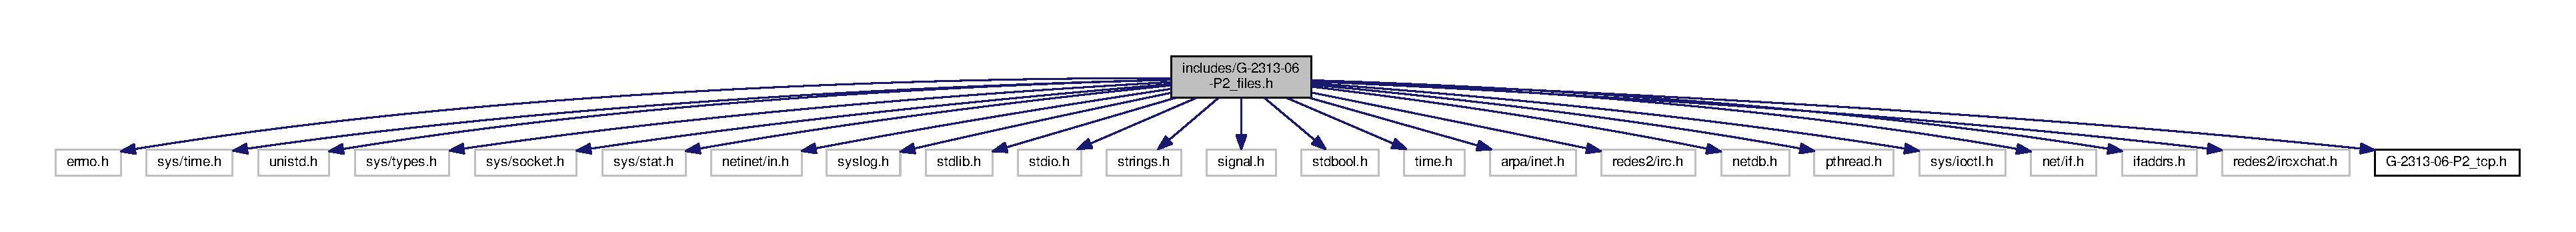
\includegraphics[width=350pt]{G-2313-06-P2__files_8h__incl}
\end{center}
\end{figure}
Gráfico de los archivos que directa o indirectamente incluyen a este archivo\+:\nopagebreak
\begin{figure}[H]
\begin{center}
\leavevmode
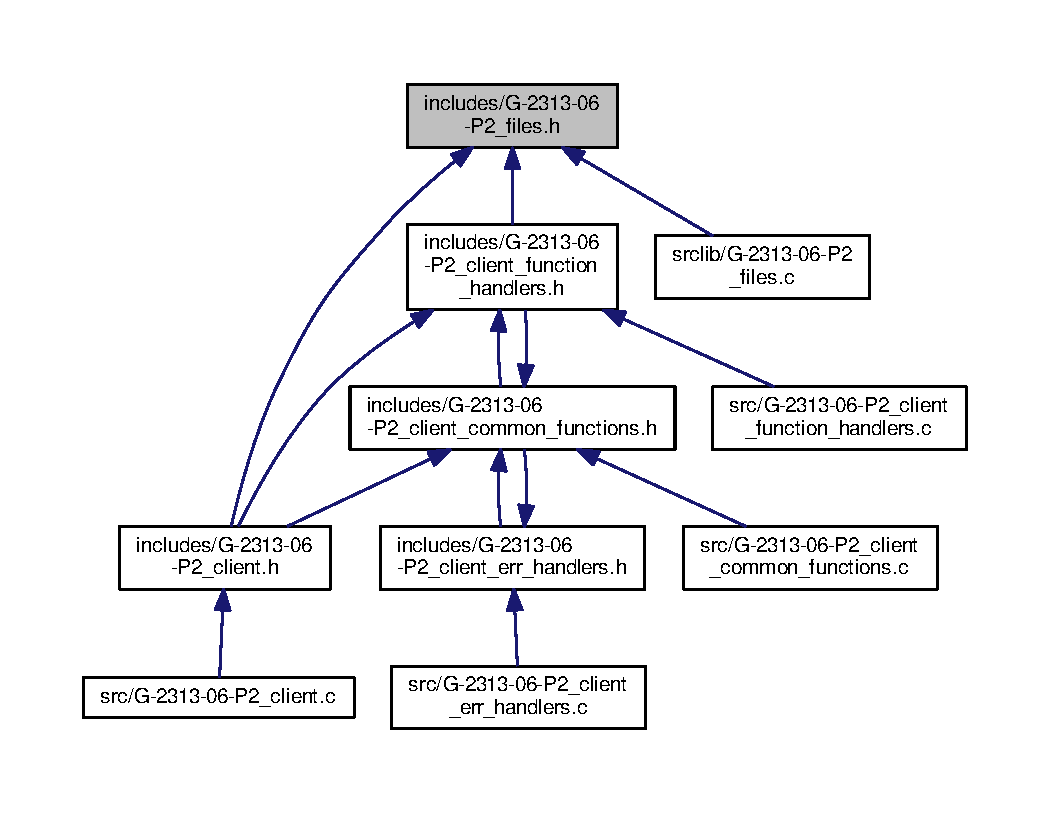
\includegraphics[width=350pt]{G-2313-06-P2__files_8h__dep__incl}
\end{center}
\end{figure}
\subsection*{Clases}
\begin{DoxyCompactItemize}
\item 
struct \hyperlink{structsrecv}{srecv}
\end{DoxyCompactItemize}
\subsection*{Funciones}
\begin{DoxyCompactItemize}
\item 
void $\ast$ \hyperlink{G-2313-06-P2__files_8h_ad00af19306b45db3947f1b89ae4b5def}{server\+\_\+especial\+\_\+enviar\+\_\+ficheros} (void $\ast$vrecv)
\item 
void $\ast$ \hyperlink{G-2313-06-P2__files_8h_a6796f20636727f52161d02748cb2b17e}{server\+\_\+especial\+\_\+recibir\+\_\+ficheros} (void $\ast$vmsg)
\end{DoxyCompactItemize}


\subsection{Documentación de las funciones}
\index{G-\/2313-\/06-\/\+P2\+\_\+files.\+h@{G-\/2313-\/06-\/\+P2\+\_\+files.\+h}!server\+\_\+especial\+\_\+enviar\+\_\+ficheros@{server\+\_\+especial\+\_\+enviar\+\_\+ficheros}}
\index{server\+\_\+especial\+\_\+enviar\+\_\+ficheros@{server\+\_\+especial\+\_\+enviar\+\_\+ficheros}!G-\/2313-\/06-\/\+P2\+\_\+files.\+h@{G-\/2313-\/06-\/\+P2\+\_\+files.\+h}}
\subsubsection[{\texorpdfstring{server\+\_\+especial\+\_\+enviar\+\_\+ficheros(void $\ast$vrecv)}{server_especial_enviar_ficheros(void *vrecv)}}]{\setlength{\rightskip}{0pt plus 5cm}void$\ast$ server\+\_\+especial\+\_\+enviar\+\_\+ficheros (
\begin{DoxyParamCaption}
\item[{void $\ast$}]{vrecv}
\end{DoxyParamCaption}
)}\hypertarget{G-2313-06-P2__files_8h_ad00af19306b45db3947f1b89ae4b5def}{}\label{G-2313-06-P2__files_8h_ad00af19306b45db3947f1b89ae4b5def}


Definición en la línea 53 del archivo G-\/2313-\/06-\/\+P2\+\_\+files.\+c.

\index{G-\/2313-\/06-\/\+P2\+\_\+files.\+h@{G-\/2313-\/06-\/\+P2\+\_\+files.\+h}!server\+\_\+especial\+\_\+recibir\+\_\+ficheros@{server\+\_\+especial\+\_\+recibir\+\_\+ficheros}}
\index{server\+\_\+especial\+\_\+recibir\+\_\+ficheros@{server\+\_\+especial\+\_\+recibir\+\_\+ficheros}!G-\/2313-\/06-\/\+P2\+\_\+files.\+h@{G-\/2313-\/06-\/\+P2\+\_\+files.\+h}}
\subsubsection[{\texorpdfstring{server\+\_\+especial\+\_\+recibir\+\_\+ficheros(void $\ast$vmsg)}{server_especial_recibir_ficheros(void *vmsg)}}]{\setlength{\rightskip}{0pt plus 5cm}void$\ast$ server\+\_\+especial\+\_\+recibir\+\_\+ficheros (
\begin{DoxyParamCaption}
\item[{void $\ast$}]{vmsg}
\end{DoxyParamCaption}
)}\hypertarget{G-2313-06-P2__files_8h_a6796f20636727f52161d02748cb2b17e}{}\label{G-2313-06-P2__files_8h_a6796f20636727f52161d02748cb2b17e}


Definición en la línea 213 del archivo G-\/2313-\/06-\/\+P2\+\_\+files.\+c.


\hypertarget{G-2313-06-P2__tcp_8h}{}\section{Referencia del Archivo includes/\+G-\/2313-\/06-\/\+P2\+\_\+tcp.h}
\label{G-2313-06-P2__tcp_8h}\index{includes/\+G-\/2313-\/06-\/\+P2\+\_\+tcp.\+h@{includes/\+G-\/2313-\/06-\/\+P2\+\_\+tcp.\+h}}
Gráfico de los archivos que directa o indirectamente incluyen a este archivo\+:\nopagebreak
\begin{figure}[H]
\begin{center}
\leavevmode
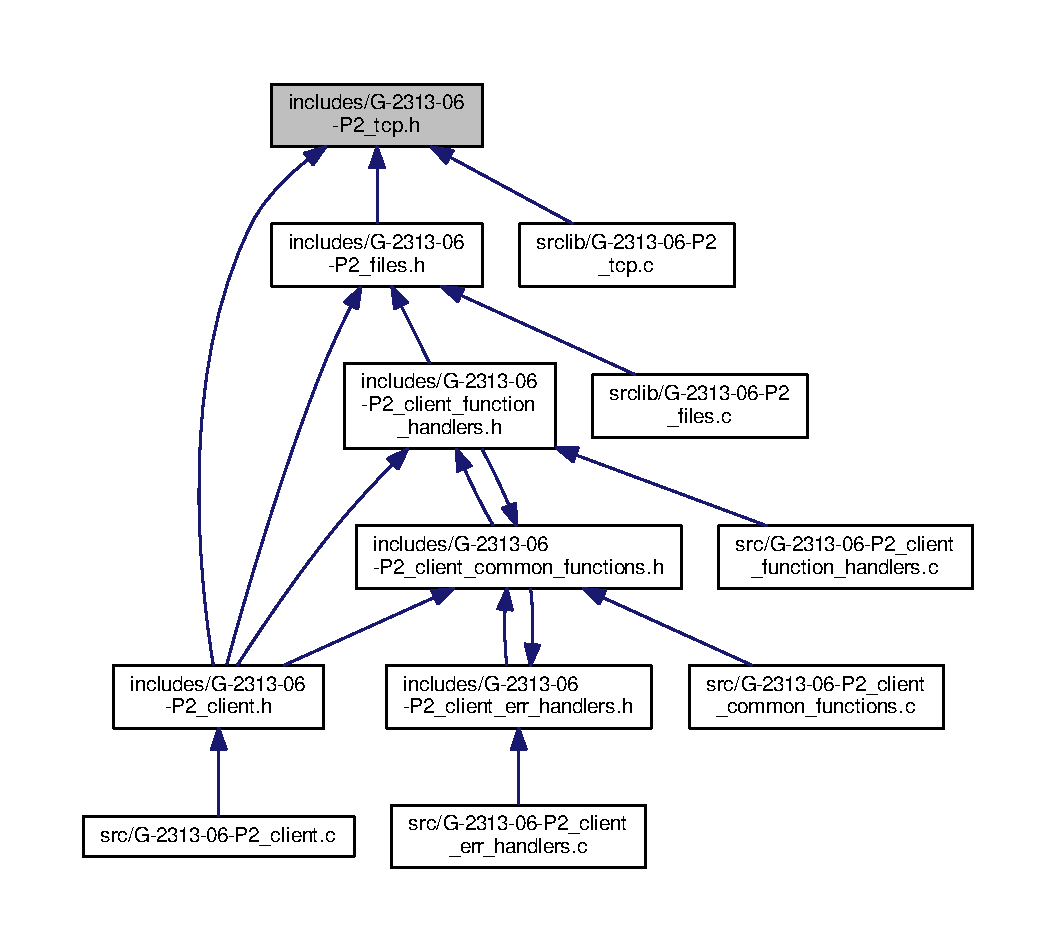
\includegraphics[width=350pt]{G-2313-06-P2__tcp_8h__dep__incl}
\end{center}
\end{figure}
\subsection*{Funciones}
\begin{DoxyCompactItemize}
\item 
int \hyperlink{G-2313-06-P2__tcp_8h_a4e5ce422aa030ac8b3998e858b79cae2}{tcp\+\_\+connect} (char $\ast$server, int port)
\item 
int \hyperlink{G-2313-06-P2__tcp_8h_a14d727cfbcd2ce3c5f4fae5a470a84da}{tcp\+\_\+listen} (int port, int max\+\_\+conn)
\item 
int \hyperlink{G-2313-06-P2__tcp_8h_a1e2b75e457a02f23d433a6821f6902b7}{tcp\+\_\+send} (int fd, char $\ast$msg)
\item 
int \hyperlink{G-2313-06-P2__tcp_8h_af3354e60e1181adcd72f9f242063fafe}{tcp\+\_\+receive} (int fd, char $\ast$msg, int len)
\item 
int \hyperlink{G-2313-06-P2__tcp_8h_a2d1f9e76e5da3a7c1e172d1294a33611}{tcp\+\_\+disconnect} (int fd)
\end{DoxyCompactItemize}


\subsection{Documentación de las funciones}
\index{G-\/2313-\/06-\/\+P2\+\_\+tcp.\+h@{G-\/2313-\/06-\/\+P2\+\_\+tcp.\+h}!tcp\+\_\+connect@{tcp\+\_\+connect}}
\index{tcp\+\_\+connect@{tcp\+\_\+connect}!G-\/2313-\/06-\/\+P2\+\_\+tcp.\+h@{G-\/2313-\/06-\/\+P2\+\_\+tcp.\+h}}
\subsubsection[{\texorpdfstring{tcp\+\_\+connect(char $\ast$server, int port)}{tcp_connect(char *server, int port)}}]{\setlength{\rightskip}{0pt plus 5cm}int tcp\+\_\+connect (
\begin{DoxyParamCaption}
\item[{char $\ast$}]{server, }
\item[{int}]{port}
\end{DoxyParamCaption}
)}\hypertarget{G-2313-06-P2__tcp_8h_a4e5ce422aa030ac8b3998e858b79cae2}{}\label{G-2313-06-P2__tcp_8h_a4e5ce422aa030ac8b3998e858b79cae2}


Definición en la línea 7 del archivo G-\/2313-\/06-\/\+P2\+\_\+tcp.\+c.

\index{G-\/2313-\/06-\/\+P2\+\_\+tcp.\+h@{G-\/2313-\/06-\/\+P2\+\_\+tcp.\+h}!tcp\+\_\+disconnect@{tcp\+\_\+disconnect}}
\index{tcp\+\_\+disconnect@{tcp\+\_\+disconnect}!G-\/2313-\/06-\/\+P2\+\_\+tcp.\+h@{G-\/2313-\/06-\/\+P2\+\_\+tcp.\+h}}
\subsubsection[{\texorpdfstring{tcp\+\_\+disconnect(int fd)}{tcp_disconnect(int fd)}}]{\setlength{\rightskip}{0pt plus 5cm}int tcp\+\_\+disconnect (
\begin{DoxyParamCaption}
\item[{int}]{fd}
\end{DoxyParamCaption}
)}\hypertarget{G-2313-06-P2__tcp_8h_a2d1f9e76e5da3a7c1e172d1294a33611}{}\label{G-2313-06-P2__tcp_8h_a2d1f9e76e5da3a7c1e172d1294a33611}


Definición en la línea 88 del archivo G-\/2313-\/06-\/\+P2\+\_\+tcp.\+c.

\index{G-\/2313-\/06-\/\+P2\+\_\+tcp.\+h@{G-\/2313-\/06-\/\+P2\+\_\+tcp.\+h}!tcp\+\_\+listen@{tcp\+\_\+listen}}
\index{tcp\+\_\+listen@{tcp\+\_\+listen}!G-\/2313-\/06-\/\+P2\+\_\+tcp.\+h@{G-\/2313-\/06-\/\+P2\+\_\+tcp.\+h}}
\subsubsection[{\texorpdfstring{tcp\+\_\+listen(int port, int max\+\_\+conn)}{tcp_listen(int port, int max_conn)}}]{\setlength{\rightskip}{0pt plus 5cm}int tcp\+\_\+listen (
\begin{DoxyParamCaption}
\item[{int}]{port, }
\item[{int}]{max\+\_\+conn}
\end{DoxyParamCaption}
)}\hypertarget{G-2313-06-P2__tcp_8h_a14d727cfbcd2ce3c5f4fae5a470a84da}{}\label{G-2313-06-P2__tcp_8h_a14d727cfbcd2ce3c5f4fae5a470a84da}


Definición en la línea 39 del archivo G-\/2313-\/06-\/\+P2\+\_\+tcp.\+c.

\index{G-\/2313-\/06-\/\+P2\+\_\+tcp.\+h@{G-\/2313-\/06-\/\+P2\+\_\+tcp.\+h}!tcp\+\_\+receive@{tcp\+\_\+receive}}
\index{tcp\+\_\+receive@{tcp\+\_\+receive}!G-\/2313-\/06-\/\+P2\+\_\+tcp.\+h@{G-\/2313-\/06-\/\+P2\+\_\+tcp.\+h}}
\subsubsection[{\texorpdfstring{tcp\+\_\+receive(int fd, char $\ast$msg, int len)}{tcp_receive(int fd, char *msg, int len)}}]{\setlength{\rightskip}{0pt plus 5cm}int tcp\+\_\+receive (
\begin{DoxyParamCaption}
\item[{int}]{fd, }
\item[{char $\ast$}]{msg, }
\item[{int}]{len}
\end{DoxyParamCaption}
)}\hypertarget{G-2313-06-P2__tcp_8h_af3354e60e1181adcd72f9f242063fafe}{}\label{G-2313-06-P2__tcp_8h_af3354e60e1181adcd72f9f242063fafe}


Definición en la línea 81 del archivo G-\/2313-\/06-\/\+P2\+\_\+tcp.\+c.

\index{G-\/2313-\/06-\/\+P2\+\_\+tcp.\+h@{G-\/2313-\/06-\/\+P2\+\_\+tcp.\+h}!tcp\+\_\+send@{tcp\+\_\+send}}
\index{tcp\+\_\+send@{tcp\+\_\+send}!G-\/2313-\/06-\/\+P2\+\_\+tcp.\+h@{G-\/2313-\/06-\/\+P2\+\_\+tcp.\+h}}
\subsubsection[{\texorpdfstring{tcp\+\_\+send(int fd, char $\ast$msg)}{tcp_send(int fd, char *msg)}}]{\setlength{\rightskip}{0pt plus 5cm}int tcp\+\_\+send (
\begin{DoxyParamCaption}
\item[{int}]{fd, }
\item[{char $\ast$}]{msg}
\end{DoxyParamCaption}
)}\hypertarget{G-2313-06-P2__tcp_8h_a1e2b75e457a02f23d433a6821f6902b7}{}\label{G-2313-06-P2__tcp_8h_a1e2b75e457a02f23d433a6821f6902b7}


Definición en la línea 74 del archivo G-\/2313-\/06-\/\+P2\+\_\+tcp.\+c.


\hypertarget{G-2313-06-P2__client_8c}{}\section{Referencia del Archivo src/\+G-\/2313-\/06-\/\+P2\+\_\+client.c}
\label{G-2313-06-P2__client_8c}\index{src/\+G-\/2313-\/06-\/\+P2\+\_\+client.\+c@{src/\+G-\/2313-\/06-\/\+P2\+\_\+client.\+c}}
{\ttfamily \#include $<$redes2/ircxchat.\+h$>$}\\*
{\ttfamily \#include \char`\"{}../includes/\+G-\/2313-\/06-\/\+P2\+\_\+client.\+h\char`\"{}}\\*
Dependencia gráfica adjunta para G-\/2313-\/06-\/\+P2\+\_\+client.c\+:\nopagebreak
\begin{figure}[H]
\begin{center}
\leavevmode
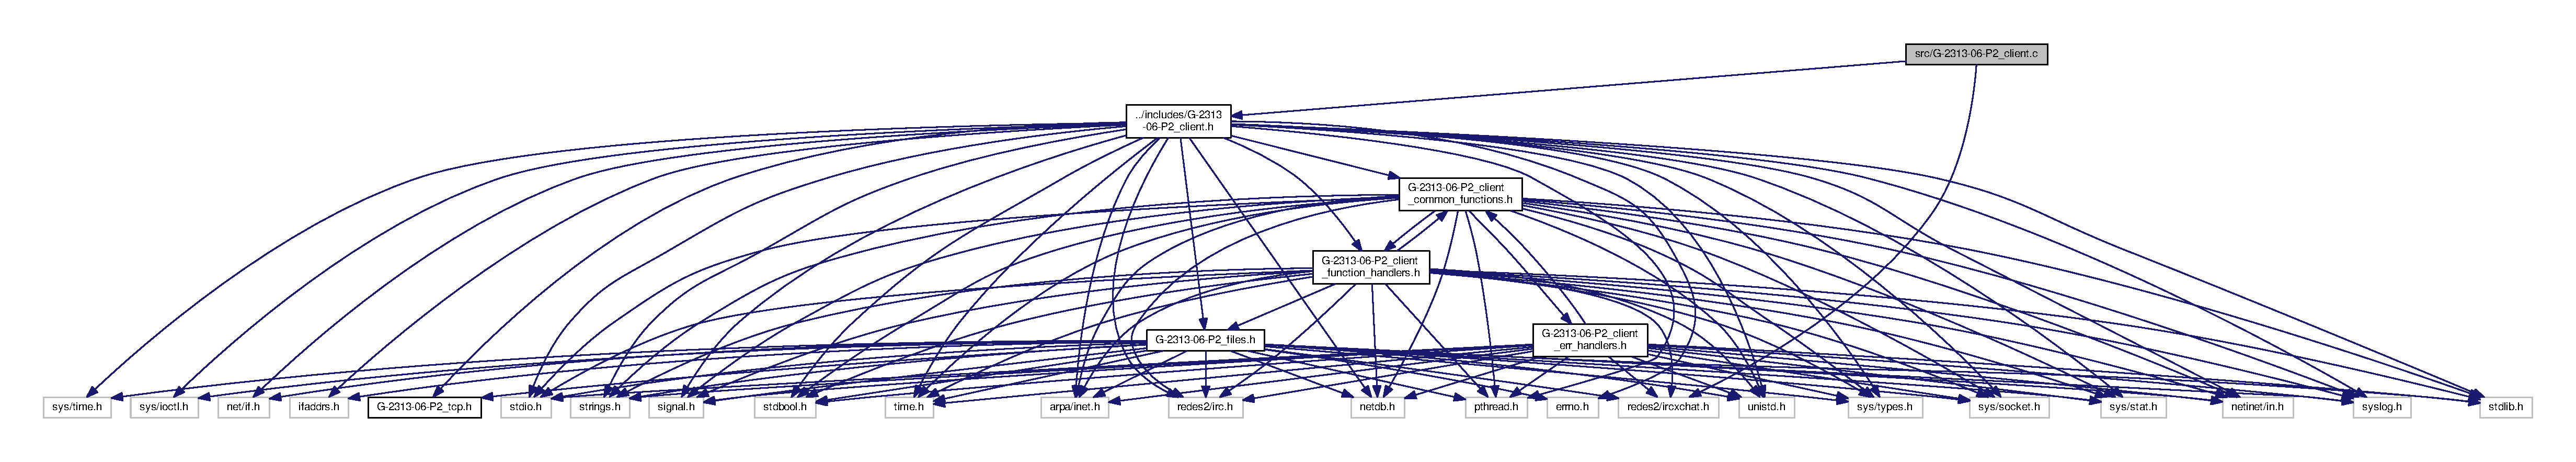
\includegraphics[width=350pt]{G-2313-06-P2__client_8c__incl}
\end{center}
\end{figure}
\subsection*{Funciones}
\begin{DoxyCompactItemize}
\item 
void \hyperlink{G-2313-06-P2__client_8c_a33f80a29a744e4182b29e23f13c1f05c}{I\+R\+C\+Interface\+\_\+\+Activate\+Channel\+Key} (char $\ast$channel, char $\ast$key)
\item 
void \hyperlink{G-2313-06-P2__client_8c_a7a439929c246e342ae525139b2c39f5d}{I\+R\+C\+Interface\+\_\+\+Activate\+External\+Messages} (char $\ast$channel)
\item 
void \hyperlink{G-2313-06-P2__client_8c_ac72762ab1e3575b421b967241db23f9c}{I\+R\+C\+Interface\+\_\+\+Activate\+Invite} (char $\ast$channel)
\item 
void \hyperlink{G-2313-06-P2__client_8c_af83498f4058311f4562c43a9b70566b2}{I\+R\+C\+Interface\+\_\+\+Activate\+Moderated} (char $\ast$channel)
\item 
void \hyperlink{G-2313-06-P2__client_8c_ab5694cc413472173bfcaa969c7d9800e}{I\+R\+C\+Interface\+\_\+\+Activate\+Nicks\+Limit} (char $\ast$channel, int limit)
\item 
void \hyperlink{G-2313-06-P2__client_8c_ab1f09c737c7c109a97e22de6072d731d}{I\+R\+C\+Interface\+\_\+\+Activate\+Private} (char $\ast$channel)
\item 
void \hyperlink{G-2313-06-P2__client_8c_ac45f12d4dcacf3b5485eec6fdc51df93}{I\+R\+C\+Interface\+\_\+\+Activate\+Protect\+Topic} (char $\ast$channel)
\item 
void \hyperlink{G-2313-06-P2__client_8c_aa9e9155115b834d85a4d10cb27f99093}{I\+R\+C\+Interface\+\_\+\+Activate\+Secret} (char $\ast$channel)
\item 
void \hyperlink{G-2313-06-P2__client_8c_a42773b5a840f9d0455f148d285e1e595}{I\+R\+C\+Interface\+\_\+\+Ban\+Nick} (char $\ast$channel, char $\ast$nick)
\item 
long \hyperlink{G-2313-06-P2__client_8c_aed072f4ce0d6e90697d4d6eb0278a2ad}{I\+R\+C\+Interface\+\_\+\+Connect} (char $\ast$nick, char $\ast$user, char $\ast$realname, char $\ast$password, char $\ast$server, int port, boolean ssl)
\item 
void \hyperlink{G-2313-06-P2__client_8c_a3e67ee0cd384b524d57fda14593dce8e}{I\+R\+C\+Interface\+\_\+\+Deactivate\+Channel\+Key} (char $\ast$channel)
\item 
void \hyperlink{G-2313-06-P2__client_8c_a638b1535f4ecbc9a6affb2df2a6a946e}{I\+R\+C\+Interface\+\_\+\+Deactivate\+External\+Messages} (char $\ast$channel)
\item 
void \hyperlink{G-2313-06-P2__client_8c_a9ba4e98a3729737aa63ebec54ba4e894}{I\+R\+C\+Interface\+\_\+\+Deactivate\+Invite} (char $\ast$channel)
\item 
void \hyperlink{G-2313-06-P2__client_8c_ab760e8144b38f6c14bd809d157cee5d4}{I\+R\+C\+Interface\+\_\+\+Deactivate\+Moderated} (char $\ast$channel)
\item 
void \hyperlink{G-2313-06-P2__client_8c_a92c8cfbe2e14e19277e1c97d11719e80}{I\+R\+C\+Interface\+\_\+\+Deactivate\+Nicks\+Limit} (char $\ast$channel)
\item 
void \hyperlink{G-2313-06-P2__client_8c_a8a6141803691ba327f11ba763ad075d4}{I\+R\+C\+Interface\+\_\+\+Deactivate\+Private} (char $\ast$channel)
\item 
void \hyperlink{G-2313-06-P2__client_8c_a5a57541a950f8c2c40b4b44c32b28ed9}{I\+R\+C\+Interface\+\_\+\+Deactivate\+Protect\+Topic} (char $\ast$channel)
\item 
void \hyperlink{G-2313-06-P2__client_8c_a4956427664cabc7d5b2bd1589a207324}{I\+R\+C\+Interface\+\_\+\+Deactivate\+Secret} (char $\ast$channel)
\item 
boolean \hyperlink{G-2313-06-P2__client_8c_a8bf0424ef7f845be79a056e9aed56fe2}{I\+R\+C\+Interface\+\_\+\+Disconnect\+Server} (char $\ast$server, int port)
\item 
boolean \hyperlink{G-2313-06-P2__client_8c_ab431412191716f751461f94d613ffdab}{I\+R\+C\+Interface\+\_\+\+Exit\+Audio\+Chat} (char $\ast$nick)
\item 
void \hyperlink{G-2313-06-P2__client_8c_ae075029bb55e8b995f22beb0810674f4}{I\+R\+C\+Interface\+\_\+\+Give\+Op} (char $\ast$channel, char $\ast$nick)
\item 
void \hyperlink{G-2313-06-P2__client_8c_ae9effb4bdaf4a2cdf2dd9edbeb90b430}{I\+R\+C\+Interface\+\_\+\+Give\+Voice} (char $\ast$channel, char $\ast$nick)
\item 
void \hyperlink{G-2313-06-P2__client_8c_a7adfea400a96160585f86179bafb055f}{I\+R\+C\+Interface\+\_\+\+Kick\+Nick} (char $\ast$channel, char $\ast$nick)
\item 
void \hyperlink{G-2313-06-P2__client_8c_a214e10b19c8be028fb35d2a7abf3f798}{I\+R\+C\+Interface\+\_\+\+New\+Command\+Text} (char $\ast$command)
\item 
void \hyperlink{G-2313-06-P2__client_8c_a080cf34ff506481737f6d08af60ca92b}{I\+R\+C\+Interface\+\_\+\+New\+Topic\+Enter} (char $\ast$topicdata)
\item 
boolean \hyperlink{G-2313-06-P2__client_8c_a100f1c87bb3b399a7284e62dd2e6172a}{I\+R\+C\+Interface\+\_\+\+Send\+File} (char $\ast$filename, char $\ast$nick, char $\ast$data, long unsigned int length)
\item 
boolean \hyperlink{G-2313-06-P2__client_8c_a5dc7a44587e609b416a783cd420a12e3}{I\+R\+C\+Interface\+\_\+\+Start\+Audio\+Chat} (char $\ast$nick)
\item 
boolean \hyperlink{G-2313-06-P2__client_8c_a754a3d3dd311194637c07cc701e7d507}{I\+R\+C\+Interface\+\_\+\+Stop\+Audio\+Chat} (char $\ast$nick)
\item 
void \hyperlink{G-2313-06-P2__client_8c_a4e2a1ea75e59306142030a91a054b7e6}{I\+R\+C\+Interface\+\_\+\+Take\+Op} (char $\ast$channel, char $\ast$nick)
\item 
void \hyperlink{G-2313-06-P2__client_8c_a2ff2e10ed1cb1a399293b6f76ac1e5ae}{I\+R\+C\+Interface\+\_\+\+Take\+Voice} (char $\ast$channel, char $\ast$nick)
\item 
int \hyperlink{G-2313-06-P2__client_8c_a0ddf1224851353fc92bfbff6f499fa97}{main} (int argc, char $\ast$argv\mbox{[}$\,$\mbox{]})
\end{DoxyCompactItemize}
\subsection*{Variables}
\begin{DoxyCompactItemize}
\item 
int \hyperlink{G-2313-06-P2__client_8c_adeadf7cb6916a10c7142ce7d265ab32a}{socket\+\_\+desc}
\item 
char $\ast$ \hyperlink{G-2313-06-P2__client_8c_ab93a317ee9a27c82844c9128a76b136a}{nick\+\_\+cliente}
\item 
pthread\+\_\+t \hyperlink{G-2313-06-P2__client_8c_a497238a5c30172237878376d95472ce4}{thread\+\_\+ficheros}
\item 
pthread\+\_\+t \hyperlink{G-2313-06-P2__client_8c_a081c16d23aa5029dd2454dfb0c355eb0}{thread\+\_\+ping}
\item 
pthread\+\_\+t \hyperlink{G-2313-06-P2__client_8c_a2b3ce8d8dc4bda71d7bd4a3b47fffd9d}{thread\+\_\+response}
\end{DoxyCompactItemize}


\subsection{Documentación de las funciones}
\index{G-\/2313-\/06-\/\+P2\+\_\+client.\+c@{G-\/2313-\/06-\/\+P2\+\_\+client.\+c}!I\+R\+C\+Interface\+\_\+\+Activate\+Channel\+Key@{I\+R\+C\+Interface\+\_\+\+Activate\+Channel\+Key}}
\index{I\+R\+C\+Interface\+\_\+\+Activate\+Channel\+Key@{I\+R\+C\+Interface\+\_\+\+Activate\+Channel\+Key}!G-\/2313-\/06-\/\+P2\+\_\+client.\+c@{G-\/2313-\/06-\/\+P2\+\_\+client.\+c}}
\subsubsection[{\texorpdfstring{I\+R\+C\+Interface\+\_\+\+Activate\+Channel\+Key(char $\ast$channel, char $\ast$key)}{IRCInterface_ActivateChannelKey(char *channel, char *key)}}]{\setlength{\rightskip}{0pt plus 5cm}void I\+R\+C\+Interface\+\_\+\+Activate\+Channel\+Key (
\begin{DoxyParamCaption}
\item[{char $\ast$}]{channel, }
\item[{char $\ast$}]{key}
\end{DoxyParamCaption}
)}\hypertarget{G-2313-06-P2__client_8c_a33f80a29a744e4182b29e23f13c1f05c}{}\label{G-2313-06-P2__client_8c_a33f80a29a744e4182b29e23f13c1f05c}


Definición en la línea 61 del archivo G-\/2313-\/06-\/\+P2\+\_\+client.\+c.

\index{G-\/2313-\/06-\/\+P2\+\_\+client.\+c@{G-\/2313-\/06-\/\+P2\+\_\+client.\+c}!I\+R\+C\+Interface\+\_\+\+Activate\+External\+Messages@{I\+R\+C\+Interface\+\_\+\+Activate\+External\+Messages}}
\index{I\+R\+C\+Interface\+\_\+\+Activate\+External\+Messages@{I\+R\+C\+Interface\+\_\+\+Activate\+External\+Messages}!G-\/2313-\/06-\/\+P2\+\_\+client.\+c@{G-\/2313-\/06-\/\+P2\+\_\+client.\+c}}
\subsubsection[{\texorpdfstring{I\+R\+C\+Interface\+\_\+\+Activate\+External\+Messages(char $\ast$channel)}{IRCInterface_ActivateExternalMessages(char *channel)}}]{\setlength{\rightskip}{0pt plus 5cm}void I\+R\+C\+Interface\+\_\+\+Activate\+External\+Messages (
\begin{DoxyParamCaption}
\item[{char $\ast$}]{channel}
\end{DoxyParamCaption}
)}\hypertarget{G-2313-06-P2__client_8c_a7a439929c246e342ae525139b2c39f5d}{}\label{G-2313-06-P2__client_8c_a7a439929c246e342ae525139b2c39f5d}


Definición en la línea 108 del archivo G-\/2313-\/06-\/\+P2\+\_\+client.\+c.

\index{G-\/2313-\/06-\/\+P2\+\_\+client.\+c@{G-\/2313-\/06-\/\+P2\+\_\+client.\+c}!I\+R\+C\+Interface\+\_\+\+Activate\+Invite@{I\+R\+C\+Interface\+\_\+\+Activate\+Invite}}
\index{I\+R\+C\+Interface\+\_\+\+Activate\+Invite@{I\+R\+C\+Interface\+\_\+\+Activate\+Invite}!G-\/2313-\/06-\/\+P2\+\_\+client.\+c@{G-\/2313-\/06-\/\+P2\+\_\+client.\+c}}
\subsubsection[{\texorpdfstring{I\+R\+C\+Interface\+\_\+\+Activate\+Invite(char $\ast$channel)}{IRCInterface_ActivateInvite(char *channel)}}]{\setlength{\rightskip}{0pt plus 5cm}void I\+R\+C\+Interface\+\_\+\+Activate\+Invite (
\begin{DoxyParamCaption}
\item[{char $\ast$}]{channel}
\end{DoxyParamCaption}
)}\hypertarget{G-2313-06-P2__client_8c_ac72762ab1e3575b421b967241db23f9c}{}\label{G-2313-06-P2__client_8c_ac72762ab1e3575b421b967241db23f9c}


Definición en la línea 156 del archivo G-\/2313-\/06-\/\+P2\+\_\+client.\+c.

\index{G-\/2313-\/06-\/\+P2\+\_\+client.\+c@{G-\/2313-\/06-\/\+P2\+\_\+client.\+c}!I\+R\+C\+Interface\+\_\+\+Activate\+Moderated@{I\+R\+C\+Interface\+\_\+\+Activate\+Moderated}}
\index{I\+R\+C\+Interface\+\_\+\+Activate\+Moderated@{I\+R\+C\+Interface\+\_\+\+Activate\+Moderated}!G-\/2313-\/06-\/\+P2\+\_\+client.\+c@{G-\/2313-\/06-\/\+P2\+\_\+client.\+c}}
\subsubsection[{\texorpdfstring{I\+R\+C\+Interface\+\_\+\+Activate\+Moderated(char $\ast$channel)}{IRCInterface_ActivateModerated(char *channel)}}]{\setlength{\rightskip}{0pt plus 5cm}void I\+R\+C\+Interface\+\_\+\+Activate\+Moderated (
\begin{DoxyParamCaption}
\item[{char $\ast$}]{channel}
\end{DoxyParamCaption}
)}\hypertarget{G-2313-06-P2__client_8c_af83498f4058311f4562c43a9b70566b2}{}\label{G-2313-06-P2__client_8c_af83498f4058311f4562c43a9b70566b2}


Definición en la línea 200 del archivo G-\/2313-\/06-\/\+P2\+\_\+client.\+c.

\index{G-\/2313-\/06-\/\+P2\+\_\+client.\+c@{G-\/2313-\/06-\/\+P2\+\_\+client.\+c}!I\+R\+C\+Interface\+\_\+\+Activate\+Nicks\+Limit@{I\+R\+C\+Interface\+\_\+\+Activate\+Nicks\+Limit}}
\index{I\+R\+C\+Interface\+\_\+\+Activate\+Nicks\+Limit@{I\+R\+C\+Interface\+\_\+\+Activate\+Nicks\+Limit}!G-\/2313-\/06-\/\+P2\+\_\+client.\+c@{G-\/2313-\/06-\/\+P2\+\_\+client.\+c}}
\subsubsection[{\texorpdfstring{I\+R\+C\+Interface\+\_\+\+Activate\+Nicks\+Limit(char $\ast$channel, int limit)}{IRCInterface_ActivateNicksLimit(char *channel, int limit)}}]{\setlength{\rightskip}{0pt plus 5cm}void I\+R\+C\+Interface\+\_\+\+Activate\+Nicks\+Limit (
\begin{DoxyParamCaption}
\item[{char $\ast$}]{channel, }
\item[{int}]{limit}
\end{DoxyParamCaption}
)}\hypertarget{G-2313-06-P2__client_8c_ab5694cc413472173bfcaa969c7d9800e}{}\label{G-2313-06-P2__client_8c_ab5694cc413472173bfcaa969c7d9800e}


Definición en la línea 251 del archivo G-\/2313-\/06-\/\+P2\+\_\+client.\+c.

\index{G-\/2313-\/06-\/\+P2\+\_\+client.\+c@{G-\/2313-\/06-\/\+P2\+\_\+client.\+c}!I\+R\+C\+Interface\+\_\+\+Activate\+Private@{I\+R\+C\+Interface\+\_\+\+Activate\+Private}}
\index{I\+R\+C\+Interface\+\_\+\+Activate\+Private@{I\+R\+C\+Interface\+\_\+\+Activate\+Private}!G-\/2313-\/06-\/\+P2\+\_\+client.\+c@{G-\/2313-\/06-\/\+P2\+\_\+client.\+c}}
\subsubsection[{\texorpdfstring{I\+R\+C\+Interface\+\_\+\+Activate\+Private(char $\ast$channel)}{IRCInterface_ActivatePrivate(char *channel)}}]{\setlength{\rightskip}{0pt plus 5cm}void I\+R\+C\+Interface\+\_\+\+Activate\+Private (
\begin{DoxyParamCaption}
\item[{char $\ast$}]{channel}
\end{DoxyParamCaption}
)}\hypertarget{G-2313-06-P2__client_8c_ab1f09c737c7c109a97e22de6072d731d}{}\label{G-2313-06-P2__client_8c_ab1f09c737c7c109a97e22de6072d731d}


Definición en la línea 300 del archivo G-\/2313-\/06-\/\+P2\+\_\+client.\+c.

\index{G-\/2313-\/06-\/\+P2\+\_\+client.\+c@{G-\/2313-\/06-\/\+P2\+\_\+client.\+c}!I\+R\+C\+Interface\+\_\+\+Activate\+Protect\+Topic@{I\+R\+C\+Interface\+\_\+\+Activate\+Protect\+Topic}}
\index{I\+R\+C\+Interface\+\_\+\+Activate\+Protect\+Topic@{I\+R\+C\+Interface\+\_\+\+Activate\+Protect\+Topic}!G-\/2313-\/06-\/\+P2\+\_\+client.\+c@{G-\/2313-\/06-\/\+P2\+\_\+client.\+c}}
\subsubsection[{\texorpdfstring{I\+R\+C\+Interface\+\_\+\+Activate\+Protect\+Topic(char $\ast$channel)}{IRCInterface_ActivateProtectTopic(char *channel)}}]{\setlength{\rightskip}{0pt plus 5cm}void I\+R\+C\+Interface\+\_\+\+Activate\+Protect\+Topic (
\begin{DoxyParamCaption}
\item[{char $\ast$}]{channel}
\end{DoxyParamCaption}
)}\hypertarget{G-2313-06-P2__client_8c_ac45f12d4dcacf3b5485eec6fdc51df93}{}\label{G-2313-06-P2__client_8c_ac45f12d4dcacf3b5485eec6fdc51df93}


Definición en la línea 344 del archivo G-\/2313-\/06-\/\+P2\+\_\+client.\+c.

\index{G-\/2313-\/06-\/\+P2\+\_\+client.\+c@{G-\/2313-\/06-\/\+P2\+\_\+client.\+c}!I\+R\+C\+Interface\+\_\+\+Activate\+Secret@{I\+R\+C\+Interface\+\_\+\+Activate\+Secret}}
\index{I\+R\+C\+Interface\+\_\+\+Activate\+Secret@{I\+R\+C\+Interface\+\_\+\+Activate\+Secret}!G-\/2313-\/06-\/\+P2\+\_\+client.\+c@{G-\/2313-\/06-\/\+P2\+\_\+client.\+c}}
\subsubsection[{\texorpdfstring{I\+R\+C\+Interface\+\_\+\+Activate\+Secret(char $\ast$channel)}{IRCInterface_ActivateSecret(char *channel)}}]{\setlength{\rightskip}{0pt plus 5cm}void I\+R\+C\+Interface\+\_\+\+Activate\+Secret (
\begin{DoxyParamCaption}
\item[{char $\ast$}]{channel}
\end{DoxyParamCaption}
)}\hypertarget{G-2313-06-P2__client_8c_aa9e9155115b834d85a4d10cb27f99093}{}\label{G-2313-06-P2__client_8c_aa9e9155115b834d85a4d10cb27f99093}


Definición en la línea 392 del archivo G-\/2313-\/06-\/\+P2\+\_\+client.\+c.

\index{G-\/2313-\/06-\/\+P2\+\_\+client.\+c@{G-\/2313-\/06-\/\+P2\+\_\+client.\+c}!I\+R\+C\+Interface\+\_\+\+Ban\+Nick@{I\+R\+C\+Interface\+\_\+\+Ban\+Nick}}
\index{I\+R\+C\+Interface\+\_\+\+Ban\+Nick@{I\+R\+C\+Interface\+\_\+\+Ban\+Nick}!G-\/2313-\/06-\/\+P2\+\_\+client.\+c@{G-\/2313-\/06-\/\+P2\+\_\+client.\+c}}
\subsubsection[{\texorpdfstring{I\+R\+C\+Interface\+\_\+\+Ban\+Nick(char $\ast$channel, char $\ast$nick)}{IRCInterface_BanNick(char *channel, char *nick)}}]{\setlength{\rightskip}{0pt plus 5cm}void I\+R\+C\+Interface\+\_\+\+Ban\+Nick (
\begin{DoxyParamCaption}
\item[{char $\ast$}]{channel, }
\item[{char $\ast$}]{nick}
\end{DoxyParamCaption}
)}\hypertarget{G-2313-06-P2__client_8c_a42773b5a840f9d0455f148d285e1e595}{}\label{G-2313-06-P2__client_8c_a42773b5a840f9d0455f148d285e1e595}


Definición en la línea 442 del archivo G-\/2313-\/06-\/\+P2\+\_\+client.\+c.

\index{G-\/2313-\/06-\/\+P2\+\_\+client.\+c@{G-\/2313-\/06-\/\+P2\+\_\+client.\+c}!I\+R\+C\+Interface\+\_\+\+Connect@{I\+R\+C\+Interface\+\_\+\+Connect}}
\index{I\+R\+C\+Interface\+\_\+\+Connect@{I\+R\+C\+Interface\+\_\+\+Connect}!G-\/2313-\/06-\/\+P2\+\_\+client.\+c@{G-\/2313-\/06-\/\+P2\+\_\+client.\+c}}
\subsubsection[{\texorpdfstring{I\+R\+C\+Interface\+\_\+\+Connect(char $\ast$nick, char $\ast$user, char $\ast$realname, char $\ast$password, char $\ast$server, int port, boolean ssl)}{IRCInterface_Connect(char *nick, char *user, char *realname, char *password, char *server, int port, boolean ssl)}}]{\setlength{\rightskip}{0pt plus 5cm}long I\+R\+C\+Interface\+\_\+\+Connect (
\begin{DoxyParamCaption}
\item[{char $\ast$}]{nick, }
\item[{char $\ast$}]{user, }
\item[{char $\ast$}]{realname, }
\item[{char $\ast$}]{password, }
\item[{char $\ast$}]{server, }
\item[{int}]{port, }
\item[{boolean}]{ssl}
\end{DoxyParamCaption}
)}\hypertarget{G-2313-06-P2__client_8c_aed072f4ce0d6e90697d4d6eb0278a2ad}{}\label{G-2313-06-P2__client_8c_aed072f4ce0d6e90697d4d6eb0278a2ad}


Definición en la línea 502 del archivo G-\/2313-\/06-\/\+P2\+\_\+client.\+c.

\index{G-\/2313-\/06-\/\+P2\+\_\+client.\+c@{G-\/2313-\/06-\/\+P2\+\_\+client.\+c}!I\+R\+C\+Interface\+\_\+\+Deactivate\+Channel\+Key@{I\+R\+C\+Interface\+\_\+\+Deactivate\+Channel\+Key}}
\index{I\+R\+C\+Interface\+\_\+\+Deactivate\+Channel\+Key@{I\+R\+C\+Interface\+\_\+\+Deactivate\+Channel\+Key}!G-\/2313-\/06-\/\+P2\+\_\+client.\+c@{G-\/2313-\/06-\/\+P2\+\_\+client.\+c}}
\subsubsection[{\texorpdfstring{I\+R\+C\+Interface\+\_\+\+Deactivate\+Channel\+Key(char $\ast$channel)}{IRCInterface_DeactivateChannelKey(char *channel)}}]{\setlength{\rightskip}{0pt plus 5cm}void I\+R\+C\+Interface\+\_\+\+Deactivate\+Channel\+Key (
\begin{DoxyParamCaption}
\item[{char $\ast$}]{channel}
\end{DoxyParamCaption}
)}\hypertarget{G-2313-06-P2__client_8c_a3e67ee0cd384b524d57fda14593dce8e}{}\label{G-2313-06-P2__client_8c_a3e67ee0cd384b524d57fda14593dce8e}


Definición en la línea 599 del archivo G-\/2313-\/06-\/\+P2\+\_\+client.\+c.

\index{G-\/2313-\/06-\/\+P2\+\_\+client.\+c@{G-\/2313-\/06-\/\+P2\+\_\+client.\+c}!I\+R\+C\+Interface\+\_\+\+Deactivate\+External\+Messages@{I\+R\+C\+Interface\+\_\+\+Deactivate\+External\+Messages}}
\index{I\+R\+C\+Interface\+\_\+\+Deactivate\+External\+Messages@{I\+R\+C\+Interface\+\_\+\+Deactivate\+External\+Messages}!G-\/2313-\/06-\/\+P2\+\_\+client.\+c@{G-\/2313-\/06-\/\+P2\+\_\+client.\+c}}
\subsubsection[{\texorpdfstring{I\+R\+C\+Interface\+\_\+\+Deactivate\+External\+Messages(char $\ast$channel)}{IRCInterface_DeactivateExternalMessages(char *channel)}}]{\setlength{\rightskip}{0pt plus 5cm}void I\+R\+C\+Interface\+\_\+\+Deactivate\+External\+Messages (
\begin{DoxyParamCaption}
\item[{char $\ast$}]{channel}
\end{DoxyParamCaption}
)}\hypertarget{G-2313-06-P2__client_8c_a638b1535f4ecbc9a6affb2df2a6a946e}{}\label{G-2313-06-P2__client_8c_a638b1535f4ecbc9a6affb2df2a6a946e}


Definición en la línea 646 del archivo G-\/2313-\/06-\/\+P2\+\_\+client.\+c.

\index{G-\/2313-\/06-\/\+P2\+\_\+client.\+c@{G-\/2313-\/06-\/\+P2\+\_\+client.\+c}!I\+R\+C\+Interface\+\_\+\+Deactivate\+Invite@{I\+R\+C\+Interface\+\_\+\+Deactivate\+Invite}}
\index{I\+R\+C\+Interface\+\_\+\+Deactivate\+Invite@{I\+R\+C\+Interface\+\_\+\+Deactivate\+Invite}!G-\/2313-\/06-\/\+P2\+\_\+client.\+c@{G-\/2313-\/06-\/\+P2\+\_\+client.\+c}}
\subsubsection[{\texorpdfstring{I\+R\+C\+Interface\+\_\+\+Deactivate\+Invite(char $\ast$channel)}{IRCInterface_DeactivateInvite(char *channel)}}]{\setlength{\rightskip}{0pt plus 5cm}void I\+R\+C\+Interface\+\_\+\+Deactivate\+Invite (
\begin{DoxyParamCaption}
\item[{char $\ast$}]{channel}
\end{DoxyParamCaption}
)}\hypertarget{G-2313-06-P2__client_8c_a9ba4e98a3729737aa63ebec54ba4e894}{}\label{G-2313-06-P2__client_8c_a9ba4e98a3729737aa63ebec54ba4e894}


Definición en la línea 693 del archivo G-\/2313-\/06-\/\+P2\+\_\+client.\+c.

\index{G-\/2313-\/06-\/\+P2\+\_\+client.\+c@{G-\/2313-\/06-\/\+P2\+\_\+client.\+c}!I\+R\+C\+Interface\+\_\+\+Deactivate\+Moderated@{I\+R\+C\+Interface\+\_\+\+Deactivate\+Moderated}}
\index{I\+R\+C\+Interface\+\_\+\+Deactivate\+Moderated@{I\+R\+C\+Interface\+\_\+\+Deactivate\+Moderated}!G-\/2313-\/06-\/\+P2\+\_\+client.\+c@{G-\/2313-\/06-\/\+P2\+\_\+client.\+c}}
\subsubsection[{\texorpdfstring{I\+R\+C\+Interface\+\_\+\+Deactivate\+Moderated(char $\ast$channel)}{IRCInterface_DeactivateModerated(char *channel)}}]{\setlength{\rightskip}{0pt plus 5cm}void I\+R\+C\+Interface\+\_\+\+Deactivate\+Moderated (
\begin{DoxyParamCaption}
\item[{char $\ast$}]{channel}
\end{DoxyParamCaption}
)}\hypertarget{G-2313-06-P2__client_8c_ab760e8144b38f6c14bd809d157cee5d4}{}\label{G-2313-06-P2__client_8c_ab760e8144b38f6c14bd809d157cee5d4}


Definición en la línea 740 del archivo G-\/2313-\/06-\/\+P2\+\_\+client.\+c.

\index{G-\/2313-\/06-\/\+P2\+\_\+client.\+c@{G-\/2313-\/06-\/\+P2\+\_\+client.\+c}!I\+R\+C\+Interface\+\_\+\+Deactivate\+Nicks\+Limit@{I\+R\+C\+Interface\+\_\+\+Deactivate\+Nicks\+Limit}}
\index{I\+R\+C\+Interface\+\_\+\+Deactivate\+Nicks\+Limit@{I\+R\+C\+Interface\+\_\+\+Deactivate\+Nicks\+Limit}!G-\/2313-\/06-\/\+P2\+\_\+client.\+c@{G-\/2313-\/06-\/\+P2\+\_\+client.\+c}}
\subsubsection[{\texorpdfstring{I\+R\+C\+Interface\+\_\+\+Deactivate\+Nicks\+Limit(char $\ast$channel)}{IRCInterface_DeactivateNicksLimit(char *channel)}}]{\setlength{\rightskip}{0pt plus 5cm}void I\+R\+C\+Interface\+\_\+\+Deactivate\+Nicks\+Limit (
\begin{DoxyParamCaption}
\item[{char $\ast$}]{channel}
\end{DoxyParamCaption}
)}\hypertarget{G-2313-06-P2__client_8c_a92c8cfbe2e14e19277e1c97d11719e80}{}\label{G-2313-06-P2__client_8c_a92c8cfbe2e14e19277e1c97d11719e80}


Definición en la línea 787 del archivo G-\/2313-\/06-\/\+P2\+\_\+client.\+c.

\index{G-\/2313-\/06-\/\+P2\+\_\+client.\+c@{G-\/2313-\/06-\/\+P2\+\_\+client.\+c}!I\+R\+C\+Interface\+\_\+\+Deactivate\+Private@{I\+R\+C\+Interface\+\_\+\+Deactivate\+Private}}
\index{I\+R\+C\+Interface\+\_\+\+Deactivate\+Private@{I\+R\+C\+Interface\+\_\+\+Deactivate\+Private}!G-\/2313-\/06-\/\+P2\+\_\+client.\+c@{G-\/2313-\/06-\/\+P2\+\_\+client.\+c}}
\subsubsection[{\texorpdfstring{I\+R\+C\+Interface\+\_\+\+Deactivate\+Private(char $\ast$channel)}{IRCInterface_DeactivatePrivate(char *channel)}}]{\setlength{\rightskip}{0pt plus 5cm}void I\+R\+C\+Interface\+\_\+\+Deactivate\+Private (
\begin{DoxyParamCaption}
\item[{char $\ast$}]{channel}
\end{DoxyParamCaption}
)}\hypertarget{G-2313-06-P2__client_8c_a8a6141803691ba327f11ba763ad075d4}{}\label{G-2313-06-P2__client_8c_a8a6141803691ba327f11ba763ad075d4}


Definición en la línea 836 del archivo G-\/2313-\/06-\/\+P2\+\_\+client.\+c.

\index{G-\/2313-\/06-\/\+P2\+\_\+client.\+c@{G-\/2313-\/06-\/\+P2\+\_\+client.\+c}!I\+R\+C\+Interface\+\_\+\+Deactivate\+Protect\+Topic@{I\+R\+C\+Interface\+\_\+\+Deactivate\+Protect\+Topic}}
\index{I\+R\+C\+Interface\+\_\+\+Deactivate\+Protect\+Topic@{I\+R\+C\+Interface\+\_\+\+Deactivate\+Protect\+Topic}!G-\/2313-\/06-\/\+P2\+\_\+client.\+c@{G-\/2313-\/06-\/\+P2\+\_\+client.\+c}}
\subsubsection[{\texorpdfstring{I\+R\+C\+Interface\+\_\+\+Deactivate\+Protect\+Topic(char $\ast$channel)}{IRCInterface_DeactivateProtectTopic(char *channel)}}]{\setlength{\rightskip}{0pt plus 5cm}void I\+R\+C\+Interface\+\_\+\+Deactivate\+Protect\+Topic (
\begin{DoxyParamCaption}
\item[{char $\ast$}]{channel}
\end{DoxyParamCaption}
)}\hypertarget{G-2313-06-P2__client_8c_a5a57541a950f8c2c40b4b44c32b28ed9}{}\label{G-2313-06-P2__client_8c_a5a57541a950f8c2c40b4b44c32b28ed9}


Definición en la línea 883 del archivo G-\/2313-\/06-\/\+P2\+\_\+client.\+c.

\index{G-\/2313-\/06-\/\+P2\+\_\+client.\+c@{G-\/2313-\/06-\/\+P2\+\_\+client.\+c}!I\+R\+C\+Interface\+\_\+\+Deactivate\+Secret@{I\+R\+C\+Interface\+\_\+\+Deactivate\+Secret}}
\index{I\+R\+C\+Interface\+\_\+\+Deactivate\+Secret@{I\+R\+C\+Interface\+\_\+\+Deactivate\+Secret}!G-\/2313-\/06-\/\+P2\+\_\+client.\+c@{G-\/2313-\/06-\/\+P2\+\_\+client.\+c}}
\subsubsection[{\texorpdfstring{I\+R\+C\+Interface\+\_\+\+Deactivate\+Secret(char $\ast$channel)}{IRCInterface_DeactivateSecret(char *channel)}}]{\setlength{\rightskip}{0pt plus 5cm}void I\+R\+C\+Interface\+\_\+\+Deactivate\+Secret (
\begin{DoxyParamCaption}
\item[{char $\ast$}]{channel}
\end{DoxyParamCaption}
)}\hypertarget{G-2313-06-P2__client_8c_a4956427664cabc7d5b2bd1589a207324}{}\label{G-2313-06-P2__client_8c_a4956427664cabc7d5b2bd1589a207324}


Definición en la línea 931 del archivo G-\/2313-\/06-\/\+P2\+\_\+client.\+c.

\index{G-\/2313-\/06-\/\+P2\+\_\+client.\+c@{G-\/2313-\/06-\/\+P2\+\_\+client.\+c}!I\+R\+C\+Interface\+\_\+\+Disconnect\+Server@{I\+R\+C\+Interface\+\_\+\+Disconnect\+Server}}
\index{I\+R\+C\+Interface\+\_\+\+Disconnect\+Server@{I\+R\+C\+Interface\+\_\+\+Disconnect\+Server}!G-\/2313-\/06-\/\+P2\+\_\+client.\+c@{G-\/2313-\/06-\/\+P2\+\_\+client.\+c}}
\subsubsection[{\texorpdfstring{I\+R\+C\+Interface\+\_\+\+Disconnect\+Server(char $\ast$server, int port)}{IRCInterface_DisconnectServer(char *server, int port)}}]{\setlength{\rightskip}{0pt plus 5cm}boolean I\+R\+C\+Interface\+\_\+\+Disconnect\+Server (
\begin{DoxyParamCaption}
\item[{char $\ast$}]{server, }
\item[{int}]{port}
\end{DoxyParamCaption}
)}\hypertarget{G-2313-06-P2__client_8c_a8bf0424ef7f845be79a056e9aed56fe2}{}\label{G-2313-06-P2__client_8c_a8bf0424ef7f845be79a056e9aed56fe2}


Definición en la línea 982 del archivo G-\/2313-\/06-\/\+P2\+\_\+client.\+c.

\index{G-\/2313-\/06-\/\+P2\+\_\+client.\+c@{G-\/2313-\/06-\/\+P2\+\_\+client.\+c}!I\+R\+C\+Interface\+\_\+\+Exit\+Audio\+Chat@{I\+R\+C\+Interface\+\_\+\+Exit\+Audio\+Chat}}
\index{I\+R\+C\+Interface\+\_\+\+Exit\+Audio\+Chat@{I\+R\+C\+Interface\+\_\+\+Exit\+Audio\+Chat}!G-\/2313-\/06-\/\+P2\+\_\+client.\+c@{G-\/2313-\/06-\/\+P2\+\_\+client.\+c}}
\subsubsection[{\texorpdfstring{I\+R\+C\+Interface\+\_\+\+Exit\+Audio\+Chat(char $\ast$nick)}{IRCInterface_ExitAudioChat(char *nick)}}]{\setlength{\rightskip}{0pt plus 5cm}boolean I\+R\+C\+Interface\+\_\+\+Exit\+Audio\+Chat (
\begin{DoxyParamCaption}
\item[{char $\ast$}]{nick}
\end{DoxyParamCaption}
)}\hypertarget{G-2313-06-P2__client_8c_ab431412191716f751461f94d613ffdab}{}\label{G-2313-06-P2__client_8c_ab431412191716f751461f94d613ffdab}


Definición en la línea 1036 del archivo G-\/2313-\/06-\/\+P2\+\_\+client.\+c.

\index{G-\/2313-\/06-\/\+P2\+\_\+client.\+c@{G-\/2313-\/06-\/\+P2\+\_\+client.\+c}!I\+R\+C\+Interface\+\_\+\+Give\+Op@{I\+R\+C\+Interface\+\_\+\+Give\+Op}}
\index{I\+R\+C\+Interface\+\_\+\+Give\+Op@{I\+R\+C\+Interface\+\_\+\+Give\+Op}!G-\/2313-\/06-\/\+P2\+\_\+client.\+c@{G-\/2313-\/06-\/\+P2\+\_\+client.\+c}}
\subsubsection[{\texorpdfstring{I\+R\+C\+Interface\+\_\+\+Give\+Op(char $\ast$channel, char $\ast$nick)}{IRCInterface_GiveOp(char *channel, char *nick)}}]{\setlength{\rightskip}{0pt plus 5cm}void I\+R\+C\+Interface\+\_\+\+Give\+Op (
\begin{DoxyParamCaption}
\item[{char $\ast$}]{channel, }
\item[{char $\ast$}]{nick}
\end{DoxyParamCaption}
)}\hypertarget{G-2313-06-P2__client_8c_ae075029bb55e8b995f22beb0810674f4}{}\label{G-2313-06-P2__client_8c_ae075029bb55e8b995f22beb0810674f4}


Definición en la línea 1073 del archivo G-\/2313-\/06-\/\+P2\+\_\+client.\+c.

\index{G-\/2313-\/06-\/\+P2\+\_\+client.\+c@{G-\/2313-\/06-\/\+P2\+\_\+client.\+c}!I\+R\+C\+Interface\+\_\+\+Give\+Voice@{I\+R\+C\+Interface\+\_\+\+Give\+Voice}}
\index{I\+R\+C\+Interface\+\_\+\+Give\+Voice@{I\+R\+C\+Interface\+\_\+\+Give\+Voice}!G-\/2313-\/06-\/\+P2\+\_\+client.\+c@{G-\/2313-\/06-\/\+P2\+\_\+client.\+c}}
\subsubsection[{\texorpdfstring{I\+R\+C\+Interface\+\_\+\+Give\+Voice(char $\ast$channel, char $\ast$nick)}{IRCInterface_GiveVoice(char *channel, char *nick)}}]{\setlength{\rightskip}{0pt plus 5cm}void I\+R\+C\+Interface\+\_\+\+Give\+Voice (
\begin{DoxyParamCaption}
\item[{char $\ast$}]{channel, }
\item[{char $\ast$}]{nick}
\end{DoxyParamCaption}
)}\hypertarget{G-2313-06-P2__client_8c_ae9effb4bdaf4a2cdf2dd9edbeb90b430}{}\label{G-2313-06-P2__client_8c_ae9effb4bdaf4a2cdf2dd9edbeb90b430}


Definición en la línea 1118 del archivo G-\/2313-\/06-\/\+P2\+\_\+client.\+c.

\index{G-\/2313-\/06-\/\+P2\+\_\+client.\+c@{G-\/2313-\/06-\/\+P2\+\_\+client.\+c}!I\+R\+C\+Interface\+\_\+\+Kick\+Nick@{I\+R\+C\+Interface\+\_\+\+Kick\+Nick}}
\index{I\+R\+C\+Interface\+\_\+\+Kick\+Nick@{I\+R\+C\+Interface\+\_\+\+Kick\+Nick}!G-\/2313-\/06-\/\+P2\+\_\+client.\+c@{G-\/2313-\/06-\/\+P2\+\_\+client.\+c}}
\subsubsection[{\texorpdfstring{I\+R\+C\+Interface\+\_\+\+Kick\+Nick(char $\ast$channel, char $\ast$nick)}{IRCInterface_KickNick(char *channel, char *nick)}}]{\setlength{\rightskip}{0pt plus 5cm}void I\+R\+C\+Interface\+\_\+\+Kick\+Nick (
\begin{DoxyParamCaption}
\item[{char $\ast$}]{channel, }
\item[{char $\ast$}]{nick}
\end{DoxyParamCaption}
)}\hypertarget{G-2313-06-P2__client_8c_a7adfea400a96160585f86179bafb055f}{}\label{G-2313-06-P2__client_8c_a7adfea400a96160585f86179bafb055f}


Definición en la línea 1163 del archivo G-\/2313-\/06-\/\+P2\+\_\+client.\+c.

\index{G-\/2313-\/06-\/\+P2\+\_\+client.\+c@{G-\/2313-\/06-\/\+P2\+\_\+client.\+c}!I\+R\+C\+Interface\+\_\+\+New\+Command\+Text@{I\+R\+C\+Interface\+\_\+\+New\+Command\+Text}}
\index{I\+R\+C\+Interface\+\_\+\+New\+Command\+Text@{I\+R\+C\+Interface\+\_\+\+New\+Command\+Text}!G-\/2313-\/06-\/\+P2\+\_\+client.\+c@{G-\/2313-\/06-\/\+P2\+\_\+client.\+c}}
\subsubsection[{\texorpdfstring{I\+R\+C\+Interface\+\_\+\+New\+Command\+Text(char $\ast$command)}{IRCInterface_NewCommandText(char *command)}}]{\setlength{\rightskip}{0pt plus 5cm}void I\+R\+C\+Interface\+\_\+\+New\+Command\+Text (
\begin{DoxyParamCaption}
\item[{char $\ast$}]{command}
\end{DoxyParamCaption}
)}\hypertarget{G-2313-06-P2__client_8c_a214e10b19c8be028fb35d2a7abf3f798}{}\label{G-2313-06-P2__client_8c_a214e10b19c8be028fb35d2a7abf3f798}


Definición en la línea 1208 del archivo G-\/2313-\/06-\/\+P2\+\_\+client.\+c.

\index{G-\/2313-\/06-\/\+P2\+\_\+client.\+c@{G-\/2313-\/06-\/\+P2\+\_\+client.\+c}!I\+R\+C\+Interface\+\_\+\+New\+Topic\+Enter@{I\+R\+C\+Interface\+\_\+\+New\+Topic\+Enter}}
\index{I\+R\+C\+Interface\+\_\+\+New\+Topic\+Enter@{I\+R\+C\+Interface\+\_\+\+New\+Topic\+Enter}!G-\/2313-\/06-\/\+P2\+\_\+client.\+c@{G-\/2313-\/06-\/\+P2\+\_\+client.\+c}}
\subsubsection[{\texorpdfstring{I\+R\+C\+Interface\+\_\+\+New\+Topic\+Enter(char $\ast$topicdata)}{IRCInterface_NewTopicEnter(char *topicdata)}}]{\setlength{\rightskip}{0pt plus 5cm}void I\+R\+C\+Interface\+\_\+\+New\+Topic\+Enter (
\begin{DoxyParamCaption}
\item[{char $\ast$}]{topicdata}
\end{DoxyParamCaption}
)}\hypertarget{G-2313-06-P2__client_8c_a080cf34ff506481737f6d08af60ca92b}{}\label{G-2313-06-P2__client_8c_a080cf34ff506481737f6d08af60ca92b}


Definición en la línea 1245 del archivo G-\/2313-\/06-\/\+P2\+\_\+client.\+c.

\index{G-\/2313-\/06-\/\+P2\+\_\+client.\+c@{G-\/2313-\/06-\/\+P2\+\_\+client.\+c}!I\+R\+C\+Interface\+\_\+\+Send\+File@{I\+R\+C\+Interface\+\_\+\+Send\+File}}
\index{I\+R\+C\+Interface\+\_\+\+Send\+File@{I\+R\+C\+Interface\+\_\+\+Send\+File}!G-\/2313-\/06-\/\+P2\+\_\+client.\+c@{G-\/2313-\/06-\/\+P2\+\_\+client.\+c}}
\subsubsection[{\texorpdfstring{I\+R\+C\+Interface\+\_\+\+Send\+File(char $\ast$filename, char $\ast$nick, char $\ast$data, long unsigned int length)}{IRCInterface_SendFile(char *filename, char *nick, char *data, long unsigned int length)}}]{\setlength{\rightskip}{0pt plus 5cm}boolean I\+R\+C\+Interface\+\_\+\+Send\+File (
\begin{DoxyParamCaption}
\item[{char $\ast$}]{filename, }
\item[{char $\ast$}]{nick, }
\item[{char $\ast$}]{data, }
\item[{long unsigned int}]{length}
\end{DoxyParamCaption}
)}\hypertarget{G-2313-06-P2__client_8c_a100f1c87bb3b399a7284e62dd2e6172a}{}\label{G-2313-06-P2__client_8c_a100f1c87bb3b399a7284e62dd2e6172a}


Definición en la línea 1298 del archivo G-\/2313-\/06-\/\+P2\+\_\+client.\+c.

\index{G-\/2313-\/06-\/\+P2\+\_\+client.\+c@{G-\/2313-\/06-\/\+P2\+\_\+client.\+c}!I\+R\+C\+Interface\+\_\+\+Start\+Audio\+Chat@{I\+R\+C\+Interface\+\_\+\+Start\+Audio\+Chat}}
\index{I\+R\+C\+Interface\+\_\+\+Start\+Audio\+Chat@{I\+R\+C\+Interface\+\_\+\+Start\+Audio\+Chat}!G-\/2313-\/06-\/\+P2\+\_\+client.\+c@{G-\/2313-\/06-\/\+P2\+\_\+client.\+c}}
\subsubsection[{\texorpdfstring{I\+R\+C\+Interface\+\_\+\+Start\+Audio\+Chat(char $\ast$nick)}{IRCInterface_StartAudioChat(char *nick)}}]{\setlength{\rightskip}{0pt plus 5cm}boolean I\+R\+C\+Interface\+\_\+\+Start\+Audio\+Chat (
\begin{DoxyParamCaption}
\item[{char $\ast$}]{nick}
\end{DoxyParamCaption}
)}\hypertarget{G-2313-06-P2__client_8c_a5dc7a44587e609b416a783cd420a12e3}{}\label{G-2313-06-P2__client_8c_a5dc7a44587e609b416a783cd420a12e3}


Definición en la línea 1356 del archivo G-\/2313-\/06-\/\+P2\+\_\+client.\+c.

\index{G-\/2313-\/06-\/\+P2\+\_\+client.\+c@{G-\/2313-\/06-\/\+P2\+\_\+client.\+c}!I\+R\+C\+Interface\+\_\+\+Stop\+Audio\+Chat@{I\+R\+C\+Interface\+\_\+\+Stop\+Audio\+Chat}}
\index{I\+R\+C\+Interface\+\_\+\+Stop\+Audio\+Chat@{I\+R\+C\+Interface\+\_\+\+Stop\+Audio\+Chat}!G-\/2313-\/06-\/\+P2\+\_\+client.\+c@{G-\/2313-\/06-\/\+P2\+\_\+client.\+c}}
\subsubsection[{\texorpdfstring{I\+R\+C\+Interface\+\_\+\+Stop\+Audio\+Chat(char $\ast$nick)}{IRCInterface_StopAudioChat(char *nick)}}]{\setlength{\rightskip}{0pt plus 5cm}boolean I\+R\+C\+Interface\+\_\+\+Stop\+Audio\+Chat (
\begin{DoxyParamCaption}
\item[{char $\ast$}]{nick}
\end{DoxyParamCaption}
)}\hypertarget{G-2313-06-P2__client_8c_a754a3d3dd311194637c07cc701e7d507}{}\label{G-2313-06-P2__client_8c_a754a3d3dd311194637c07cc701e7d507}


Definición en la línea 1396 del archivo G-\/2313-\/06-\/\+P2\+\_\+client.\+c.

\index{G-\/2313-\/06-\/\+P2\+\_\+client.\+c@{G-\/2313-\/06-\/\+P2\+\_\+client.\+c}!I\+R\+C\+Interface\+\_\+\+Take\+Op@{I\+R\+C\+Interface\+\_\+\+Take\+Op}}
\index{I\+R\+C\+Interface\+\_\+\+Take\+Op@{I\+R\+C\+Interface\+\_\+\+Take\+Op}!G-\/2313-\/06-\/\+P2\+\_\+client.\+c@{G-\/2313-\/06-\/\+P2\+\_\+client.\+c}}
\subsubsection[{\texorpdfstring{I\+R\+C\+Interface\+\_\+\+Take\+Op(char $\ast$channel, char $\ast$nick)}{IRCInterface_TakeOp(char *channel, char *nick)}}]{\setlength{\rightskip}{0pt plus 5cm}void I\+R\+C\+Interface\+\_\+\+Take\+Op (
\begin{DoxyParamCaption}
\item[{char $\ast$}]{channel, }
\item[{char $\ast$}]{nick}
\end{DoxyParamCaption}
)}\hypertarget{G-2313-06-P2__client_8c_a4e2a1ea75e59306142030a91a054b7e6}{}\label{G-2313-06-P2__client_8c_a4e2a1ea75e59306142030a91a054b7e6}


Definición en la línea 1433 del archivo G-\/2313-\/06-\/\+P2\+\_\+client.\+c.

\index{G-\/2313-\/06-\/\+P2\+\_\+client.\+c@{G-\/2313-\/06-\/\+P2\+\_\+client.\+c}!I\+R\+C\+Interface\+\_\+\+Take\+Voice@{I\+R\+C\+Interface\+\_\+\+Take\+Voice}}
\index{I\+R\+C\+Interface\+\_\+\+Take\+Voice@{I\+R\+C\+Interface\+\_\+\+Take\+Voice}!G-\/2313-\/06-\/\+P2\+\_\+client.\+c@{G-\/2313-\/06-\/\+P2\+\_\+client.\+c}}
\subsubsection[{\texorpdfstring{I\+R\+C\+Interface\+\_\+\+Take\+Voice(char $\ast$channel, char $\ast$nick)}{IRCInterface_TakeVoice(char *channel, char *nick)}}]{\setlength{\rightskip}{0pt plus 5cm}void I\+R\+C\+Interface\+\_\+\+Take\+Voice (
\begin{DoxyParamCaption}
\item[{char $\ast$}]{channel, }
\item[{char $\ast$}]{nick}
\end{DoxyParamCaption}
)}\hypertarget{G-2313-06-P2__client_8c_a2ff2e10ed1cb1a399293b6f76ac1e5ae}{}\label{G-2313-06-P2__client_8c_a2ff2e10ed1cb1a399293b6f76ac1e5ae}


Definición en la línea 1478 del archivo G-\/2313-\/06-\/\+P2\+\_\+client.\+c.

\index{G-\/2313-\/06-\/\+P2\+\_\+client.\+c@{G-\/2313-\/06-\/\+P2\+\_\+client.\+c}!main@{main}}
\index{main@{main}!G-\/2313-\/06-\/\+P2\+\_\+client.\+c@{G-\/2313-\/06-\/\+P2\+\_\+client.\+c}}
\subsubsection[{\texorpdfstring{main(int argc, char $\ast$argv[])}{main(int argc, char *argv[])}}]{\setlength{\rightskip}{0pt plus 5cm}int main (
\begin{DoxyParamCaption}
\item[{int}]{argc, }
\item[{char $\ast$}]{argv\mbox{[}$\,$\mbox{]}}
\end{DoxyParamCaption}
)}\hypertarget{G-2313-06-P2__client_8c_a0ddf1224851353fc92bfbff6f499fa97}{}\label{G-2313-06-P2__client_8c_a0ddf1224851353fc92bfbff6f499fa97}
M\+M\+M\+M\+M\+M\+M\+M\+MM M\+M\+M\+MM A\+A\+A\+A\+A\+AA I\+I\+I\+I\+I\+II N\+N\+N\+N\+N\+N\+N\+N\+NN N\+N\+N\+N\+NN M\+M\+M\+M\+M\+M\+M\+M\+MM M\+M\+M\+MM A\+A\+A\+A\+A\+A\+AA I\+I\+I\+II N\+N\+N\+N\+N\+N\+N\+N\+NN N\+N\+NN M\+M\+M\+MM M\+M\+MM MM MM A\+A\+A\+AA AA I\+II N\+N\+N\+NN N\+N\+NN NN M\+M\+M\+MM M\+M\+MM MM MM A\+A\+A\+AA AA I\+II N\+N\+N\+NN N\+N\+NN NN M\+M\+M\+MM M\+M\+MM MM MM A\+A\+A\+AA AA I\+II N\+N\+N\+NN N\+N\+NN NN M\+M\+M\+MM M\+M\+MM MM MM A\+A\+A\+AA AA I\+II N\+N\+N\+NN N\+N\+NN NN M\+M\+M\+MM M\+M\+MM MM MM A\+A\+A\+AA AA I\+II N\+N\+N\+NN N\+N\+NN NN M\+M\+M\+MM M\+M\+MM MM MM A\+A\+A\+A\+A\+A\+A\+A\+A\+A\+A\+A\+AA I\+II N\+N\+N\+NN N\+N\+NN NN M\+M\+M\+MM M\+M\+M\+MM MM A\+A\+A\+AA AA I\+II N\+N\+N\+NN N\+N\+NN NN M\+M\+M\+MM M\+MM MM A\+A\+A\+AA AA I\+II N\+N\+N\+NN N\+N\+NN NN M\+M\+M\+MM MM A\+A\+A\+AA AA I\+II N\+N\+N\+NN N\+N\+NN NN M\+M\+M\+MM MM A\+A\+A\+AA AA I\+II N\+N\+N\+NN N\+N\+NN NN M\+M\+M\+M\+M\+MM M\+M\+MM A\+A\+A\+A\+AA A\+A\+AA I\+I\+I\+II N\+N\+N\+N\+NN N\+N\+N\+N\+N\+NN M\+M\+M\+M\+M\+M\+M\+MM M\+M\+M\+M\+MM A\+A\+A\+A\+A\+A\+AA A\+A\+A\+A\+AA I\+I\+I\+I\+I\+II N\+N\+N\+N\+N\+NN N\+N\+N\+N\+N\+NN 

Definición en la línea 1515 del archivo G-\/2313-\/06-\/\+P2\+\_\+client.\+c.



\subsection{Documentación de las variables}
\index{G-\/2313-\/06-\/\+P2\+\_\+client.\+c@{G-\/2313-\/06-\/\+P2\+\_\+client.\+c}!nick\+\_\+cliente@{nick\+\_\+cliente}}
\index{nick\+\_\+cliente@{nick\+\_\+cliente}!G-\/2313-\/06-\/\+P2\+\_\+client.\+c@{G-\/2313-\/06-\/\+P2\+\_\+client.\+c}}
\subsubsection[{\texorpdfstring{nick\+\_\+cliente}{nick_cliente}}]{\setlength{\rightskip}{0pt plus 5cm}char$\ast$ nick\+\_\+cliente}\hypertarget{G-2313-06-P2__client_8c_ab93a317ee9a27c82844c9128a76b136a}{}\label{G-2313-06-P2__client_8c_ab93a317ee9a27c82844c9128a76b136a}


Definición en la línea 5 del archivo G-\/2313-\/06-\/\+P2\+\_\+client.\+c.

\index{G-\/2313-\/06-\/\+P2\+\_\+client.\+c@{G-\/2313-\/06-\/\+P2\+\_\+client.\+c}!socket\+\_\+desc@{socket\+\_\+desc}}
\index{socket\+\_\+desc@{socket\+\_\+desc}!G-\/2313-\/06-\/\+P2\+\_\+client.\+c@{G-\/2313-\/06-\/\+P2\+\_\+client.\+c}}
\subsubsection[{\texorpdfstring{socket\+\_\+desc}{socket_desc}}]{\setlength{\rightskip}{0pt plus 5cm}int socket\+\_\+desc}\hypertarget{G-2313-06-P2__client_8c_adeadf7cb6916a10c7142ce7d265ab32a}{}\label{G-2313-06-P2__client_8c_adeadf7cb6916a10c7142ce7d265ab32a}


Definición en la línea 4 del archivo G-\/2313-\/06-\/\+P2\+\_\+client.\+c.

\index{G-\/2313-\/06-\/\+P2\+\_\+client.\+c@{G-\/2313-\/06-\/\+P2\+\_\+client.\+c}!thread\+\_\+ficheros@{thread\+\_\+ficheros}}
\index{thread\+\_\+ficheros@{thread\+\_\+ficheros}!G-\/2313-\/06-\/\+P2\+\_\+client.\+c@{G-\/2313-\/06-\/\+P2\+\_\+client.\+c}}
\subsubsection[{\texorpdfstring{thread\+\_\+ficheros}{thread_ficheros}}]{\setlength{\rightskip}{0pt plus 5cm}pthread\+\_\+t thread\+\_\+ficheros}\hypertarget{G-2313-06-P2__client_8c_a497238a5c30172237878376d95472ce4}{}\label{G-2313-06-P2__client_8c_a497238a5c30172237878376d95472ce4}


Definición en la línea 6 del archivo G-\/2313-\/06-\/\+P2\+\_\+client.\+c.

\index{G-\/2313-\/06-\/\+P2\+\_\+client.\+c@{G-\/2313-\/06-\/\+P2\+\_\+client.\+c}!thread\+\_\+ping@{thread\+\_\+ping}}
\index{thread\+\_\+ping@{thread\+\_\+ping}!G-\/2313-\/06-\/\+P2\+\_\+client.\+c@{G-\/2313-\/06-\/\+P2\+\_\+client.\+c}}
\subsubsection[{\texorpdfstring{thread\+\_\+ping}{thread_ping}}]{\setlength{\rightskip}{0pt plus 5cm}pthread\+\_\+t thread\+\_\+ping}\hypertarget{G-2313-06-P2__client_8c_a081c16d23aa5029dd2454dfb0c355eb0}{}\label{G-2313-06-P2__client_8c_a081c16d23aa5029dd2454dfb0c355eb0}


Definición en la línea 6 del archivo G-\/2313-\/06-\/\+P2\+\_\+client.\+c.

\index{G-\/2313-\/06-\/\+P2\+\_\+client.\+c@{G-\/2313-\/06-\/\+P2\+\_\+client.\+c}!thread\+\_\+response@{thread\+\_\+response}}
\index{thread\+\_\+response@{thread\+\_\+response}!G-\/2313-\/06-\/\+P2\+\_\+client.\+c@{G-\/2313-\/06-\/\+P2\+\_\+client.\+c}}
\subsubsection[{\texorpdfstring{thread\+\_\+response}{thread_response}}]{\setlength{\rightskip}{0pt plus 5cm}pthread\+\_\+t thread\+\_\+response}\hypertarget{G-2313-06-P2__client_8c_a2b3ce8d8dc4bda71d7bd4a3b47fffd9d}{}\label{G-2313-06-P2__client_8c_a2b3ce8d8dc4bda71d7bd4a3b47fffd9d}


Definición en la línea 6 del archivo G-\/2313-\/06-\/\+P2\+\_\+client.\+c.


\hypertarget{G-2313-06-P2__client__common__functions_8c}{}\section{Referencia del Archivo src/\+G-\/2313-\/06-\/\+P2\+\_\+client\+\_\+common\+\_\+functions.c}
\label{G-2313-06-P2__client__common__functions_8c}\index{src/\+G-\/2313-\/06-\/\+P2\+\_\+client\+\_\+common\+\_\+functions.\+c@{src/\+G-\/2313-\/06-\/\+P2\+\_\+client\+\_\+common\+\_\+functions.\+c}}
{\ttfamily \#include \char`\"{}../includes/\+G-\/2313-\/06-\/\+P2\+\_\+client\+\_\+common\+\_\+functions.\+h\char`\"{}}\\*
Dependencia gráfica adjunta para G-\/2313-\/06-\/\+P2\+\_\+client\+\_\+common\+\_\+functions.c\+:\nopagebreak
\begin{figure}[H]
\begin{center}
\leavevmode
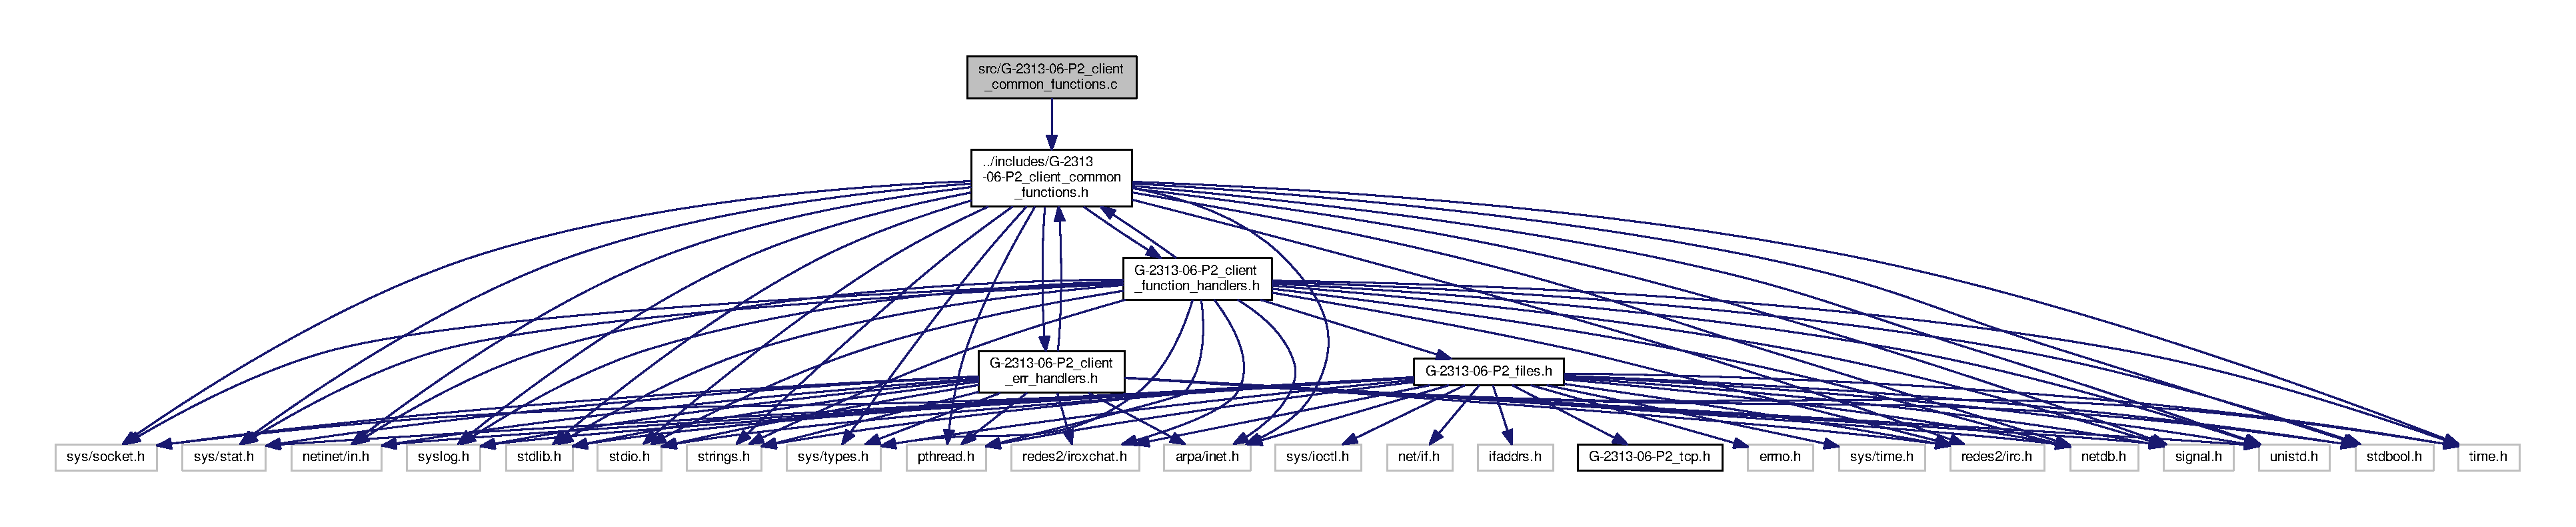
\includegraphics[width=350pt]{G-2313-06-P2__client__common__functions_8c__incl}
\end{center}
\end{figure}
\subsection*{Funciones}
\begin{DoxyCompactItemize}
\item 
void $\ast$ \hyperlink{G-2313-06-P2__client__common__functions_8c_a7297f848d5b0bd4990857d03cf3111e4}{client\+\_\+function\+\_\+ping} (void $\ast$arg)
\item 
void $\ast$ \hyperlink{G-2313-06-P2__client__common__functions_8c_afbd2dc7b3224fc3d2c5c9233b307c376}{client\+\_\+function\+\_\+response} (void $\ast$arg)
\item 
void \hyperlink{G-2313-06-P2__client__common__functions_8c_a03942275c5a503be4f7288cda71fb139}{client\+\_\+show\+\_\+error} (char $\ast$msg)
\item 
void \hyperlink{G-2313-06-P2__client__common__functions_8c_aa1f1dfdb0122f771b6c56edab7bc3613}{client\+\_\+show\+\_\+error\+\_\+main} (char $\ast$msg)
\item 
void \hyperlink{G-2313-06-P2__client__common__functions_8c_aa74c686c447b275e6a8cf36419033e81}{client\+\_\+pre\+\_\+in\+\_\+function} (char $\ast$command)
\item 
void \hyperlink{G-2313-06-P2__client__common__functions_8c_a6dd72e0b56b87f85d8cac2a30066198b}{client\+\_\+execute\+\_\+in\+\_\+function} (long function\+Name, char $\ast$command)
\item 
void \hyperlink{G-2313-06-P2__client__common__functions_8c_a68019fe1e0edcc71bb3dadeb70a86dcd}{client\+\_\+pre\+\_\+out\+\_\+function} (char $\ast$command)
\item 
void \hyperlink{G-2313-06-P2__client__common__functions_8c_a26512d35b24fec46c8fa4c803dc00867}{client\+\_\+execute\+\_\+out\+\_\+function} (long function\+Name, char $\ast$command)
\end{DoxyCompactItemize}
\subsection*{Variables}
\begin{DoxyCompactItemize}
\item 
int \hyperlink{G-2313-06-P2__client__common__functions_8c_adeadf7cb6916a10c7142ce7d265ab32a}{socket\+\_\+desc}
\end{DoxyCompactItemize}


\subsection{Documentación de las funciones}
\index{G-\/2313-\/06-\/\+P2\+\_\+client\+\_\+common\+\_\+functions.\+c@{G-\/2313-\/06-\/\+P2\+\_\+client\+\_\+common\+\_\+functions.\+c}!client\+\_\+execute\+\_\+in\+\_\+function@{client\+\_\+execute\+\_\+in\+\_\+function}}
\index{client\+\_\+execute\+\_\+in\+\_\+function@{client\+\_\+execute\+\_\+in\+\_\+function}!G-\/2313-\/06-\/\+P2\+\_\+client\+\_\+common\+\_\+functions.\+c@{G-\/2313-\/06-\/\+P2\+\_\+client\+\_\+common\+\_\+functions.\+c}}
\subsubsection[{\texorpdfstring{client\+\_\+execute\+\_\+in\+\_\+function(long function\+Name, char $\ast$command)}{client_execute_in_function(long functionName, char *command)}}]{\setlength{\rightskip}{0pt plus 5cm}void client\+\_\+execute\+\_\+in\+\_\+function (
\begin{DoxyParamCaption}
\item[{long}]{function\+Name, }
\item[{char $\ast$}]{command}
\end{DoxyParamCaption}
)}\hypertarget{G-2313-06-P2__client__common__functions_8c_a6dd72e0b56b87f85d8cac2a30066198b}{}\label{G-2313-06-P2__client__common__functions_8c_a6dd72e0b56b87f85d8cac2a30066198b}


Definición en la línea 420 del archivo G-\/2313-\/06-\/\+P2\+\_\+client\+\_\+common\+\_\+functions.\+c.

\index{G-\/2313-\/06-\/\+P2\+\_\+client\+\_\+common\+\_\+functions.\+c@{G-\/2313-\/06-\/\+P2\+\_\+client\+\_\+common\+\_\+functions.\+c}!client\+\_\+execute\+\_\+out\+\_\+function@{client\+\_\+execute\+\_\+out\+\_\+function}}
\index{client\+\_\+execute\+\_\+out\+\_\+function@{client\+\_\+execute\+\_\+out\+\_\+function}!G-\/2313-\/06-\/\+P2\+\_\+client\+\_\+common\+\_\+functions.\+c@{G-\/2313-\/06-\/\+P2\+\_\+client\+\_\+common\+\_\+functions.\+c}}
\subsubsection[{\texorpdfstring{client\+\_\+execute\+\_\+out\+\_\+function(long function\+Name, char $\ast$command)}{client_execute_out_function(long functionName, char *command)}}]{\setlength{\rightskip}{0pt plus 5cm}void client\+\_\+execute\+\_\+out\+\_\+function (
\begin{DoxyParamCaption}
\item[{long}]{function\+Name, }
\item[{char $\ast$}]{command}
\end{DoxyParamCaption}
)}\hypertarget{G-2313-06-P2__client__common__functions_8c_a26512d35b24fec46c8fa4c803dc00867}{}\label{G-2313-06-P2__client__common__functions_8c_a26512d35b24fec46c8fa4c803dc00867}


Definición en la línea 582 del archivo G-\/2313-\/06-\/\+P2\+\_\+client\+\_\+common\+\_\+functions.\+c.

\index{G-\/2313-\/06-\/\+P2\+\_\+client\+\_\+common\+\_\+functions.\+c@{G-\/2313-\/06-\/\+P2\+\_\+client\+\_\+common\+\_\+functions.\+c}!client\+\_\+function\+\_\+ping@{client\+\_\+function\+\_\+ping}}
\index{client\+\_\+function\+\_\+ping@{client\+\_\+function\+\_\+ping}!G-\/2313-\/06-\/\+P2\+\_\+client\+\_\+common\+\_\+functions.\+c@{G-\/2313-\/06-\/\+P2\+\_\+client\+\_\+common\+\_\+functions.\+c}}
\subsubsection[{\texorpdfstring{client\+\_\+function\+\_\+ping(void $\ast$arg)}{client_function_ping(void *arg)}}]{\setlength{\rightskip}{0pt plus 5cm}void$\ast$ client\+\_\+function\+\_\+ping (
\begin{DoxyParamCaption}
\item[{void $\ast$}]{arg}
\end{DoxyParamCaption}
)}\hypertarget{G-2313-06-P2__client__common__functions_8c_a7297f848d5b0bd4990857d03cf3111e4}{}\label{G-2313-06-P2__client__common__functions_8c_a7297f848d5b0bd4990857d03cf3111e4}


Definición en la línea 192 del archivo G-\/2313-\/06-\/\+P2\+\_\+client\+\_\+common\+\_\+functions.\+c.

\index{G-\/2313-\/06-\/\+P2\+\_\+client\+\_\+common\+\_\+functions.\+c@{G-\/2313-\/06-\/\+P2\+\_\+client\+\_\+common\+\_\+functions.\+c}!client\+\_\+function\+\_\+response@{client\+\_\+function\+\_\+response}}
\index{client\+\_\+function\+\_\+response@{client\+\_\+function\+\_\+response}!G-\/2313-\/06-\/\+P2\+\_\+client\+\_\+common\+\_\+functions.\+c@{G-\/2313-\/06-\/\+P2\+\_\+client\+\_\+common\+\_\+functions.\+c}}
\subsubsection[{\texorpdfstring{client\+\_\+function\+\_\+response(void $\ast$arg)}{client_function_response(void *arg)}}]{\setlength{\rightskip}{0pt plus 5cm}void$\ast$ client\+\_\+function\+\_\+response (
\begin{DoxyParamCaption}
\item[{void $\ast$}]{arg}
\end{DoxyParamCaption}
)}\hypertarget{G-2313-06-P2__client__common__functions_8c_afbd2dc7b3224fc3d2c5c9233b307c376}{}\label{G-2313-06-P2__client__common__functions_8c_afbd2dc7b3224fc3d2c5c9233b307c376}


Definición en la línea 244 del archivo G-\/2313-\/06-\/\+P2\+\_\+client\+\_\+common\+\_\+functions.\+c.

\index{G-\/2313-\/06-\/\+P2\+\_\+client\+\_\+common\+\_\+functions.\+c@{G-\/2313-\/06-\/\+P2\+\_\+client\+\_\+common\+\_\+functions.\+c}!client\+\_\+pre\+\_\+in\+\_\+function@{client\+\_\+pre\+\_\+in\+\_\+function}}
\index{client\+\_\+pre\+\_\+in\+\_\+function@{client\+\_\+pre\+\_\+in\+\_\+function}!G-\/2313-\/06-\/\+P2\+\_\+client\+\_\+common\+\_\+functions.\+c@{G-\/2313-\/06-\/\+P2\+\_\+client\+\_\+common\+\_\+functions.\+c}}
\subsubsection[{\texorpdfstring{client\+\_\+pre\+\_\+in\+\_\+function(char $\ast$command)}{client_pre_in_function(char *command)}}]{\setlength{\rightskip}{0pt plus 5cm}void client\+\_\+pre\+\_\+in\+\_\+function (
\begin{DoxyParamCaption}
\item[{char $\ast$}]{command}
\end{DoxyParamCaption}
)}\hypertarget{G-2313-06-P2__client__common__functions_8c_aa74c686c447b275e6a8cf36419033e81}{}\label{G-2313-06-P2__client__common__functions_8c_aa74c686c447b275e6a8cf36419033e81}


Definición en la línea 323 del archivo G-\/2313-\/06-\/\+P2\+\_\+client\+\_\+common\+\_\+functions.\+c.

\index{G-\/2313-\/06-\/\+P2\+\_\+client\+\_\+common\+\_\+functions.\+c@{G-\/2313-\/06-\/\+P2\+\_\+client\+\_\+common\+\_\+functions.\+c}!client\+\_\+pre\+\_\+out\+\_\+function@{client\+\_\+pre\+\_\+out\+\_\+function}}
\index{client\+\_\+pre\+\_\+out\+\_\+function@{client\+\_\+pre\+\_\+out\+\_\+function}!G-\/2313-\/06-\/\+P2\+\_\+client\+\_\+common\+\_\+functions.\+c@{G-\/2313-\/06-\/\+P2\+\_\+client\+\_\+common\+\_\+functions.\+c}}
\subsubsection[{\texorpdfstring{client\+\_\+pre\+\_\+out\+\_\+function(char $\ast$command)}{client_pre_out_function(char *command)}}]{\setlength{\rightskip}{0pt plus 5cm}void client\+\_\+pre\+\_\+out\+\_\+function (
\begin{DoxyParamCaption}
\item[{char $\ast$}]{command}
\end{DoxyParamCaption}
)}\hypertarget{G-2313-06-P2__client__common__functions_8c_a68019fe1e0edcc71bb3dadeb70a86dcd}{}\label{G-2313-06-P2__client__common__functions_8c_a68019fe1e0edcc71bb3dadeb70a86dcd}


Definición en la línea 528 del archivo G-\/2313-\/06-\/\+P2\+\_\+client\+\_\+common\+\_\+functions.\+c.

\index{G-\/2313-\/06-\/\+P2\+\_\+client\+\_\+common\+\_\+functions.\+c@{G-\/2313-\/06-\/\+P2\+\_\+client\+\_\+common\+\_\+functions.\+c}!client\+\_\+show\+\_\+error@{client\+\_\+show\+\_\+error}}
\index{client\+\_\+show\+\_\+error@{client\+\_\+show\+\_\+error}!G-\/2313-\/06-\/\+P2\+\_\+client\+\_\+common\+\_\+functions.\+c@{G-\/2313-\/06-\/\+P2\+\_\+client\+\_\+common\+\_\+functions.\+c}}
\subsubsection[{\texorpdfstring{client\+\_\+show\+\_\+error(char $\ast$msg)}{client_show_error(char *msg)}}]{\setlength{\rightskip}{0pt plus 5cm}void client\+\_\+show\+\_\+error (
\begin{DoxyParamCaption}
\item[{char $\ast$}]{msg}
\end{DoxyParamCaption}
)}\hypertarget{G-2313-06-P2__client__common__functions_8c_a03942275c5a503be4f7288cda71fb139}{}\label{G-2313-06-P2__client__common__functions_8c_a03942275c5a503be4f7288cda71fb139}


Definición en la línea 274 del archivo G-\/2313-\/06-\/\+P2\+\_\+client\+\_\+common\+\_\+functions.\+c.

\index{G-\/2313-\/06-\/\+P2\+\_\+client\+\_\+common\+\_\+functions.\+c@{G-\/2313-\/06-\/\+P2\+\_\+client\+\_\+common\+\_\+functions.\+c}!client\+\_\+show\+\_\+error\+\_\+main@{client\+\_\+show\+\_\+error\+\_\+main}}
\index{client\+\_\+show\+\_\+error\+\_\+main@{client\+\_\+show\+\_\+error\+\_\+main}!G-\/2313-\/06-\/\+P2\+\_\+client\+\_\+common\+\_\+functions.\+c@{G-\/2313-\/06-\/\+P2\+\_\+client\+\_\+common\+\_\+functions.\+c}}
\subsubsection[{\texorpdfstring{client\+\_\+show\+\_\+error\+\_\+main(char $\ast$msg)}{client_show_error_main(char *msg)}}]{\setlength{\rightskip}{0pt plus 5cm}void client\+\_\+show\+\_\+error\+\_\+main (
\begin{DoxyParamCaption}
\item[{char $\ast$}]{msg}
\end{DoxyParamCaption}
)}\hypertarget{G-2313-06-P2__client__common__functions_8c_aa1f1dfdb0122f771b6c56edab7bc3613}{}\label{G-2313-06-P2__client__common__functions_8c_aa1f1dfdb0122f771b6c56edab7bc3613}


Definición en la línea 284 del archivo G-\/2313-\/06-\/\+P2\+\_\+client\+\_\+common\+\_\+functions.\+c.



\subsection{Documentación de las variables}
\index{G-\/2313-\/06-\/\+P2\+\_\+client\+\_\+common\+\_\+functions.\+c@{G-\/2313-\/06-\/\+P2\+\_\+client\+\_\+common\+\_\+functions.\+c}!socket\+\_\+desc@{socket\+\_\+desc}}
\index{socket\+\_\+desc@{socket\+\_\+desc}!G-\/2313-\/06-\/\+P2\+\_\+client\+\_\+common\+\_\+functions.\+c@{G-\/2313-\/06-\/\+P2\+\_\+client\+\_\+common\+\_\+functions.\+c}}
\subsubsection[{\texorpdfstring{socket\+\_\+desc}{socket_desc}}]{\setlength{\rightskip}{0pt plus 5cm}int socket\+\_\+desc}\hypertarget{G-2313-06-P2__client__common__functions_8c_adeadf7cb6916a10c7142ce7d265ab32a}{}\label{G-2313-06-P2__client__common__functions_8c_adeadf7cb6916a10c7142ce7d265ab32a}


Definición en la línea 4 del archivo G-\/2313-\/06-\/\+P2\+\_\+client.\+c.


\hypertarget{G-2313-06-P2__client__err__handlers_8c}{}\section{Referencia del Archivo src/\+G-\/2313-\/06-\/\+P2\+\_\+client\+\_\+err\+\_\+handlers.c}
\label{G-2313-06-P2__client__err__handlers_8c}\index{src/\+G-\/2313-\/06-\/\+P2\+\_\+client\+\_\+err\+\_\+handlers.\+c@{src/\+G-\/2313-\/06-\/\+P2\+\_\+client\+\_\+err\+\_\+handlers.\+c}}
{\ttfamily \#include \char`\"{}../includes/\+G-\/2313-\/06-\/\+P2\+\_\+client\+\_\+err\+\_\+handlers.\+h\char`\"{}}\\*
Dependencia gráfica adjunta para G-\/2313-\/06-\/\+P2\+\_\+client\+\_\+err\+\_\+handlers.c\+:\nopagebreak
\begin{figure}[H]
\begin{center}
\leavevmode
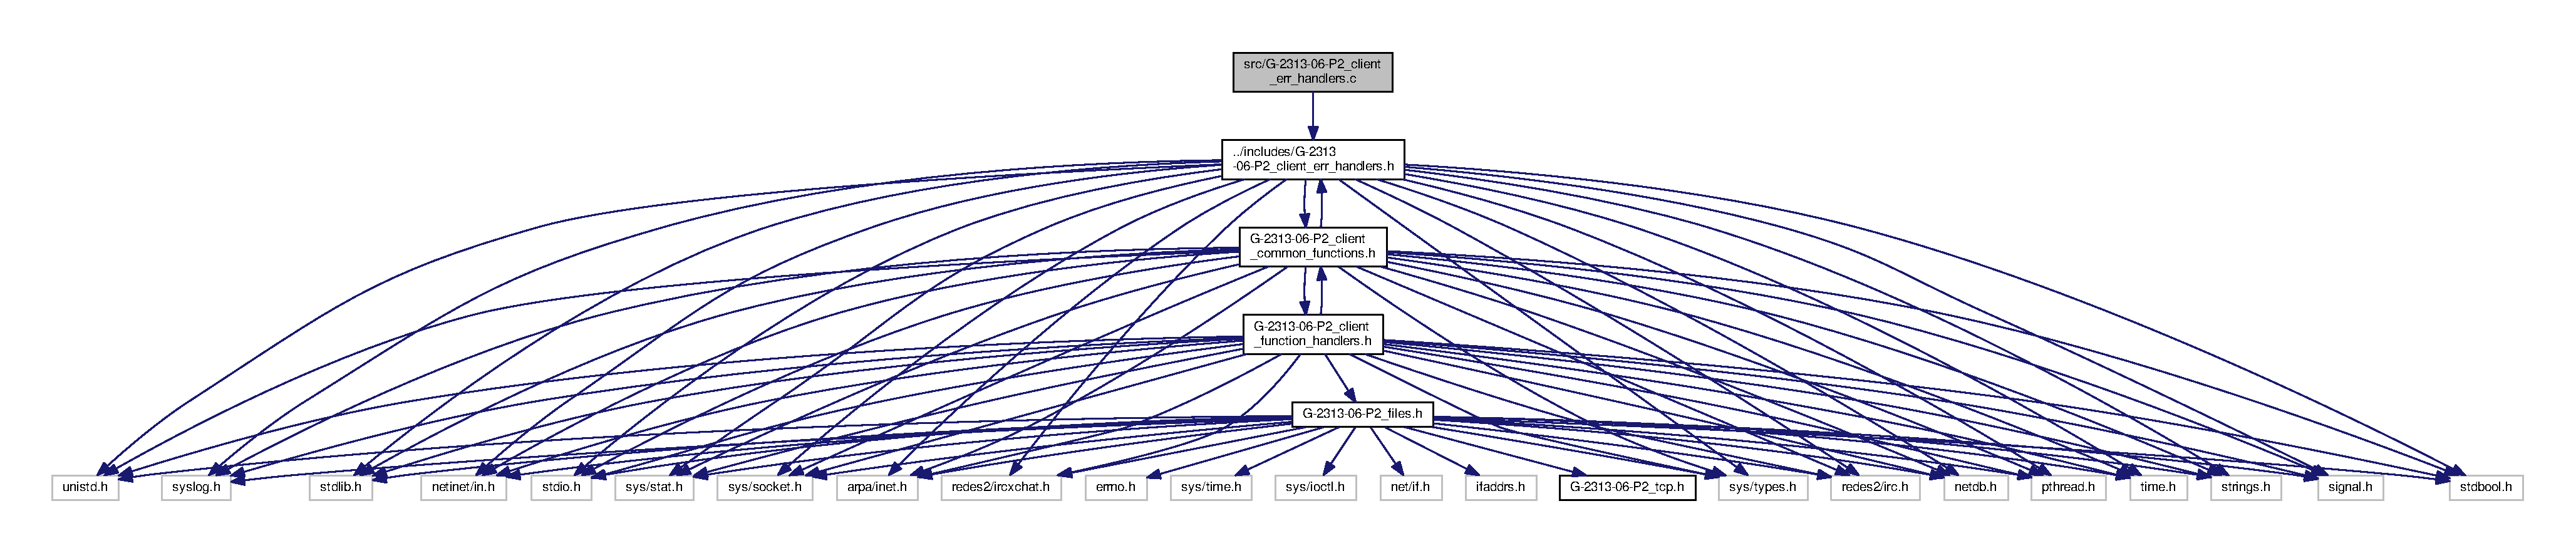
\includegraphics[width=350pt]{G-2313-06-P2__client__err__handlers_8c__incl}
\end{center}
\end{figure}
\subsection*{Funciones}
\begin{DoxyCompactItemize}
\item 
void \hyperlink{G-2313-06-P2__client__err__handlers_8c_aee5973ae831d1c7c63b1a62b59f561c2}{server\+\_\+in\+\_\+command\+\_\+err\+\_\+cannotsendtochan} (char $\ast$command)
\item 
void \hyperlink{G-2313-06-P2__client__err__handlers_8c_a14bfb17eb95d0f2bef1869aa2ebf520c}{server\+\_\+in\+\_\+command\+\_\+err\+\_\+alreadyregistred} (char $\ast$command)
\item 
void \hyperlink{G-2313-06-P2__client__err__handlers_8c_aaa9cfb1b5050bd1218c227d8d0a041fe}{server\+\_\+in\+\_\+command\+\_\+err\+\_\+nonicknamegiven} (char $\ast$command)
\item 
void \hyperlink{G-2313-06-P2__client__err__handlers_8c_abeb8ead21ebba982eb59f161eda735cb}{server\+\_\+in\+\_\+command\+\_\+err\+\_\+erroneusnickname} (char $\ast$command)
\item 
void \hyperlink{G-2313-06-P2__client__err__handlers_8c_ab6d8f2d05566bf6ee9dfcfc4a20f5d23}{server\+\_\+in\+\_\+command\+\_\+err\+\_\+nicknameinuse} (char $\ast$command)
\item 
void \hyperlink{G-2313-06-P2__client__err__handlers_8c_a4af95b292b293c08c0989b4e7334c7eb}{server\+\_\+in\+\_\+command\+\_\+err\+\_\+nickcollision} (char $\ast$command)
\item 
void \hyperlink{G-2313-06-P2__client__err__handlers_8c_ae4fcb567dc7685f5d7a4abbc7c6506b4}{server\+\_\+in\+\_\+command\+\_\+err\+\_\+unavailresource} (char $\ast$command)
\item 
void \hyperlink{G-2313-06-P2__client__err__handlers_8c_ada432444f58d5effbb05fd558a8ce289}{server\+\_\+in\+\_\+command\+\_\+err\+\_\+restricted} (char $\ast$command)
\item 
void \hyperlink{G-2313-06-P2__client__err__handlers_8c_a548a7ad35236521dca4b829e466f3379}{server\+\_\+in\+\_\+command\+\_\+err\+\_\+passwdmismatch} (char $\ast$command)
\item 
void \hyperlink{G-2313-06-P2__client__err__handlers_8c_a0e4059ef132eaac2218fdd89b20ca852}{server\+\_\+in\+\_\+command\+\_\+err\+\_\+bannedfromchan} (char $\ast$command)
\item 
void \hyperlink{G-2313-06-P2__client__err__handlers_8c_a05db0aa32f2ec2925cba3b952435bf59}{server\+\_\+in\+\_\+command\+\_\+err\+\_\+channelisfull} (char $\ast$command)
\item 
void \hyperlink{G-2313-06-P2__client__err__handlers_8c_a9fcb3f66fbcc994c7a78b36ebc0fe63d}{server\+\_\+in\+\_\+command\+\_\+err\+\_\+chanoprivsneeded} (char $\ast$command)
\item 
void \hyperlink{G-2313-06-P2__client__err__handlers_8c_ae5512c3dd8e1584fd8bafc4f5dd15d8c}{server\+\_\+in\+\_\+command\+\_\+err\+\_\+inviteonlychan} (char $\ast$command)
\item 
void \hyperlink{G-2313-06-P2__client__err__handlers_8c_aade31864807344a9961ffdab697b5727}{server\+\_\+in\+\_\+command\+\_\+err\+\_\+nochanmodes} (char $\ast$command)
\item 
void \hyperlink{G-2313-06-P2__client__err__handlers_8c_a83109e15e2a8f93c9523a84a546098c0}{server\+\_\+in\+\_\+command\+\_\+err\+\_\+nosuchchannel} (char $\ast$command)
\item 
void \hyperlink{G-2313-06-P2__client__err__handlers_8c_af262f3569e06c21e3e466266fa4e2c80}{server\+\_\+in\+\_\+command\+\_\+err\+\_\+unknownmode} (char $\ast$command)
\item 
void \hyperlink{G-2313-06-P2__client__err__handlers_8c_a678f368edc1fd437f5f115ef897bdcd9}{server\+\_\+in\+\_\+command\+\_\+err\+\_\+nomotd} (char $\ast$command)
\item 
void \hyperlink{G-2313-06-P2__client__err__handlers_8c_a01f8c9822aac18d5424ebbaf67c06a51}{server\+\_\+in\+\_\+command\+\_\+err\+\_\+nosuchnick} (char $\ast$command)
\end{DoxyCompactItemize}
\subsection*{Variables}
\begin{DoxyCompactItemize}
\item 
int \hyperlink{G-2313-06-P2__client__err__handlers_8c_adeadf7cb6916a10c7142ce7d265ab32a}{socket\+\_\+desc}
\item 
char $\ast$ \hyperlink{G-2313-06-P2__client__err__handlers_8c_ab93a317ee9a27c82844c9128a76b136a}{nick\+\_\+cliente}
\end{DoxyCompactItemize}


\subsection{Documentación de las funciones}
\index{G-\/2313-\/06-\/\+P2\+\_\+client\+\_\+err\+\_\+handlers.\+c@{G-\/2313-\/06-\/\+P2\+\_\+client\+\_\+err\+\_\+handlers.\+c}!server\+\_\+in\+\_\+command\+\_\+err\+\_\+alreadyregistred@{server\+\_\+in\+\_\+command\+\_\+err\+\_\+alreadyregistred}}
\index{server\+\_\+in\+\_\+command\+\_\+err\+\_\+alreadyregistred@{server\+\_\+in\+\_\+command\+\_\+err\+\_\+alreadyregistred}!G-\/2313-\/06-\/\+P2\+\_\+client\+\_\+err\+\_\+handlers.\+c@{G-\/2313-\/06-\/\+P2\+\_\+client\+\_\+err\+\_\+handlers.\+c}}
\subsubsection[{\texorpdfstring{server\+\_\+in\+\_\+command\+\_\+err\+\_\+alreadyregistred(char $\ast$command)}{server_in_command_err_alreadyregistred(char *command)}}]{\setlength{\rightskip}{0pt plus 5cm}void server\+\_\+in\+\_\+command\+\_\+err\+\_\+alreadyregistred (
\begin{DoxyParamCaption}
\item[{char $\ast$}]{command}
\end{DoxyParamCaption}
)}\hypertarget{G-2313-06-P2__client__err__handlers_8c_a14bfb17eb95d0f2bef1869aa2ebf520c}{}\label{G-2313-06-P2__client__err__handlers_8c_a14bfb17eb95d0f2bef1869aa2ebf520c}


Definición en la línea 17 del archivo G-\/2313-\/06-\/\+P2\+\_\+client\+\_\+err\+\_\+handlers.\+c.

\index{G-\/2313-\/06-\/\+P2\+\_\+client\+\_\+err\+\_\+handlers.\+c@{G-\/2313-\/06-\/\+P2\+\_\+client\+\_\+err\+\_\+handlers.\+c}!server\+\_\+in\+\_\+command\+\_\+err\+\_\+bannedfromchan@{server\+\_\+in\+\_\+command\+\_\+err\+\_\+bannedfromchan}}
\index{server\+\_\+in\+\_\+command\+\_\+err\+\_\+bannedfromchan@{server\+\_\+in\+\_\+command\+\_\+err\+\_\+bannedfromchan}!G-\/2313-\/06-\/\+P2\+\_\+client\+\_\+err\+\_\+handlers.\+c@{G-\/2313-\/06-\/\+P2\+\_\+client\+\_\+err\+\_\+handlers.\+c}}
\subsubsection[{\texorpdfstring{server\+\_\+in\+\_\+command\+\_\+err\+\_\+bannedfromchan(char $\ast$command)}{server_in_command_err_bannedfromchan(char *command)}}]{\setlength{\rightskip}{0pt plus 5cm}void server\+\_\+in\+\_\+command\+\_\+err\+\_\+bannedfromchan (
\begin{DoxyParamCaption}
\item[{char $\ast$}]{command}
\end{DoxyParamCaption}
)}\hypertarget{G-2313-06-P2__client__err__handlers_8c_a0e4059ef132eaac2218fdd89b20ca852}{}\label{G-2313-06-P2__client__err__handlers_8c_a0e4059ef132eaac2218fdd89b20ca852}


Definición en la línea 97 del archivo G-\/2313-\/06-\/\+P2\+\_\+client\+\_\+err\+\_\+handlers.\+c.

\index{G-\/2313-\/06-\/\+P2\+\_\+client\+\_\+err\+\_\+handlers.\+c@{G-\/2313-\/06-\/\+P2\+\_\+client\+\_\+err\+\_\+handlers.\+c}!server\+\_\+in\+\_\+command\+\_\+err\+\_\+cannotsendtochan@{server\+\_\+in\+\_\+command\+\_\+err\+\_\+cannotsendtochan}}
\index{server\+\_\+in\+\_\+command\+\_\+err\+\_\+cannotsendtochan@{server\+\_\+in\+\_\+command\+\_\+err\+\_\+cannotsendtochan}!G-\/2313-\/06-\/\+P2\+\_\+client\+\_\+err\+\_\+handlers.\+c@{G-\/2313-\/06-\/\+P2\+\_\+client\+\_\+err\+\_\+handlers.\+c}}
\subsubsection[{\texorpdfstring{server\+\_\+in\+\_\+command\+\_\+err\+\_\+cannotsendtochan(char $\ast$command)}{server_in_command_err_cannotsendtochan(char *command)}}]{\setlength{\rightskip}{0pt plus 5cm}void server\+\_\+in\+\_\+command\+\_\+err\+\_\+cannotsendtochan (
\begin{DoxyParamCaption}
\item[{char $\ast$}]{command}
\end{DoxyParamCaption}
)}\hypertarget{G-2313-06-P2__client__err__handlers_8c_aee5973ae831d1c7c63b1a62b59f561c2}{}\label{G-2313-06-P2__client__err__handlers_8c_aee5973ae831d1c7c63b1a62b59f561c2}


Definición en la línea 7 del archivo G-\/2313-\/06-\/\+P2\+\_\+client\+\_\+err\+\_\+handlers.\+c.

\index{G-\/2313-\/06-\/\+P2\+\_\+client\+\_\+err\+\_\+handlers.\+c@{G-\/2313-\/06-\/\+P2\+\_\+client\+\_\+err\+\_\+handlers.\+c}!server\+\_\+in\+\_\+command\+\_\+err\+\_\+channelisfull@{server\+\_\+in\+\_\+command\+\_\+err\+\_\+channelisfull}}
\index{server\+\_\+in\+\_\+command\+\_\+err\+\_\+channelisfull@{server\+\_\+in\+\_\+command\+\_\+err\+\_\+channelisfull}!G-\/2313-\/06-\/\+P2\+\_\+client\+\_\+err\+\_\+handlers.\+c@{G-\/2313-\/06-\/\+P2\+\_\+client\+\_\+err\+\_\+handlers.\+c}}
\subsubsection[{\texorpdfstring{server\+\_\+in\+\_\+command\+\_\+err\+\_\+channelisfull(char $\ast$command)}{server_in_command_err_channelisfull(char *command)}}]{\setlength{\rightskip}{0pt plus 5cm}void server\+\_\+in\+\_\+command\+\_\+err\+\_\+channelisfull (
\begin{DoxyParamCaption}
\item[{char $\ast$}]{command}
\end{DoxyParamCaption}
)}\hypertarget{G-2313-06-P2__client__err__handlers_8c_a05db0aa32f2ec2925cba3b952435bf59}{}\label{G-2313-06-P2__client__err__handlers_8c_a05db0aa32f2ec2925cba3b952435bf59}


Definición en la línea 107 del archivo G-\/2313-\/06-\/\+P2\+\_\+client\+\_\+err\+\_\+handlers.\+c.

\index{G-\/2313-\/06-\/\+P2\+\_\+client\+\_\+err\+\_\+handlers.\+c@{G-\/2313-\/06-\/\+P2\+\_\+client\+\_\+err\+\_\+handlers.\+c}!server\+\_\+in\+\_\+command\+\_\+err\+\_\+chanoprivsneeded@{server\+\_\+in\+\_\+command\+\_\+err\+\_\+chanoprivsneeded}}
\index{server\+\_\+in\+\_\+command\+\_\+err\+\_\+chanoprivsneeded@{server\+\_\+in\+\_\+command\+\_\+err\+\_\+chanoprivsneeded}!G-\/2313-\/06-\/\+P2\+\_\+client\+\_\+err\+\_\+handlers.\+c@{G-\/2313-\/06-\/\+P2\+\_\+client\+\_\+err\+\_\+handlers.\+c}}
\subsubsection[{\texorpdfstring{server\+\_\+in\+\_\+command\+\_\+err\+\_\+chanoprivsneeded(char $\ast$command)}{server_in_command_err_chanoprivsneeded(char *command)}}]{\setlength{\rightskip}{0pt plus 5cm}void server\+\_\+in\+\_\+command\+\_\+err\+\_\+chanoprivsneeded (
\begin{DoxyParamCaption}
\item[{char $\ast$}]{command}
\end{DoxyParamCaption}
)}\hypertarget{G-2313-06-P2__client__err__handlers_8c_a9fcb3f66fbcc994c7a78b36ebc0fe63d}{}\label{G-2313-06-P2__client__err__handlers_8c_a9fcb3f66fbcc994c7a78b36ebc0fe63d}


Definición en la línea 117 del archivo G-\/2313-\/06-\/\+P2\+\_\+client\+\_\+err\+\_\+handlers.\+c.

\index{G-\/2313-\/06-\/\+P2\+\_\+client\+\_\+err\+\_\+handlers.\+c@{G-\/2313-\/06-\/\+P2\+\_\+client\+\_\+err\+\_\+handlers.\+c}!server\+\_\+in\+\_\+command\+\_\+err\+\_\+erroneusnickname@{server\+\_\+in\+\_\+command\+\_\+err\+\_\+erroneusnickname}}
\index{server\+\_\+in\+\_\+command\+\_\+err\+\_\+erroneusnickname@{server\+\_\+in\+\_\+command\+\_\+err\+\_\+erroneusnickname}!G-\/2313-\/06-\/\+P2\+\_\+client\+\_\+err\+\_\+handlers.\+c@{G-\/2313-\/06-\/\+P2\+\_\+client\+\_\+err\+\_\+handlers.\+c}}
\subsubsection[{\texorpdfstring{server\+\_\+in\+\_\+command\+\_\+err\+\_\+erroneusnickname(char $\ast$command)}{server_in_command_err_erroneusnickname(char *command)}}]{\setlength{\rightskip}{0pt plus 5cm}void server\+\_\+in\+\_\+command\+\_\+err\+\_\+erroneusnickname (
\begin{DoxyParamCaption}
\item[{char $\ast$}]{command}
\end{DoxyParamCaption}
)}\hypertarget{G-2313-06-P2__client__err__handlers_8c_abeb8ead21ebba982eb59f161eda735cb}{}\label{G-2313-06-P2__client__err__handlers_8c_abeb8ead21ebba982eb59f161eda735cb}


Definición en la línea 37 del archivo G-\/2313-\/06-\/\+P2\+\_\+client\+\_\+err\+\_\+handlers.\+c.

\index{G-\/2313-\/06-\/\+P2\+\_\+client\+\_\+err\+\_\+handlers.\+c@{G-\/2313-\/06-\/\+P2\+\_\+client\+\_\+err\+\_\+handlers.\+c}!server\+\_\+in\+\_\+command\+\_\+err\+\_\+inviteonlychan@{server\+\_\+in\+\_\+command\+\_\+err\+\_\+inviteonlychan}}
\index{server\+\_\+in\+\_\+command\+\_\+err\+\_\+inviteonlychan@{server\+\_\+in\+\_\+command\+\_\+err\+\_\+inviteonlychan}!G-\/2313-\/06-\/\+P2\+\_\+client\+\_\+err\+\_\+handlers.\+c@{G-\/2313-\/06-\/\+P2\+\_\+client\+\_\+err\+\_\+handlers.\+c}}
\subsubsection[{\texorpdfstring{server\+\_\+in\+\_\+command\+\_\+err\+\_\+inviteonlychan(char $\ast$command)}{server_in_command_err_inviteonlychan(char *command)}}]{\setlength{\rightskip}{0pt plus 5cm}void server\+\_\+in\+\_\+command\+\_\+err\+\_\+inviteonlychan (
\begin{DoxyParamCaption}
\item[{char $\ast$}]{command}
\end{DoxyParamCaption}
)}\hypertarget{G-2313-06-P2__client__err__handlers_8c_ae5512c3dd8e1584fd8bafc4f5dd15d8c}{}\label{G-2313-06-P2__client__err__handlers_8c_ae5512c3dd8e1584fd8bafc4f5dd15d8c}


Definición en la línea 127 del archivo G-\/2313-\/06-\/\+P2\+\_\+client\+\_\+err\+\_\+handlers.\+c.

\index{G-\/2313-\/06-\/\+P2\+\_\+client\+\_\+err\+\_\+handlers.\+c@{G-\/2313-\/06-\/\+P2\+\_\+client\+\_\+err\+\_\+handlers.\+c}!server\+\_\+in\+\_\+command\+\_\+err\+\_\+nickcollision@{server\+\_\+in\+\_\+command\+\_\+err\+\_\+nickcollision}}
\index{server\+\_\+in\+\_\+command\+\_\+err\+\_\+nickcollision@{server\+\_\+in\+\_\+command\+\_\+err\+\_\+nickcollision}!G-\/2313-\/06-\/\+P2\+\_\+client\+\_\+err\+\_\+handlers.\+c@{G-\/2313-\/06-\/\+P2\+\_\+client\+\_\+err\+\_\+handlers.\+c}}
\subsubsection[{\texorpdfstring{server\+\_\+in\+\_\+command\+\_\+err\+\_\+nickcollision(char $\ast$command)}{server_in_command_err_nickcollision(char *command)}}]{\setlength{\rightskip}{0pt plus 5cm}void server\+\_\+in\+\_\+command\+\_\+err\+\_\+nickcollision (
\begin{DoxyParamCaption}
\item[{char $\ast$}]{command}
\end{DoxyParamCaption}
)}\hypertarget{G-2313-06-P2__client__err__handlers_8c_a4af95b292b293c08c0989b4e7334c7eb}{}\label{G-2313-06-P2__client__err__handlers_8c_a4af95b292b293c08c0989b4e7334c7eb}


Definición en la línea 57 del archivo G-\/2313-\/06-\/\+P2\+\_\+client\+\_\+err\+\_\+handlers.\+c.

\index{G-\/2313-\/06-\/\+P2\+\_\+client\+\_\+err\+\_\+handlers.\+c@{G-\/2313-\/06-\/\+P2\+\_\+client\+\_\+err\+\_\+handlers.\+c}!server\+\_\+in\+\_\+command\+\_\+err\+\_\+nicknameinuse@{server\+\_\+in\+\_\+command\+\_\+err\+\_\+nicknameinuse}}
\index{server\+\_\+in\+\_\+command\+\_\+err\+\_\+nicknameinuse@{server\+\_\+in\+\_\+command\+\_\+err\+\_\+nicknameinuse}!G-\/2313-\/06-\/\+P2\+\_\+client\+\_\+err\+\_\+handlers.\+c@{G-\/2313-\/06-\/\+P2\+\_\+client\+\_\+err\+\_\+handlers.\+c}}
\subsubsection[{\texorpdfstring{server\+\_\+in\+\_\+command\+\_\+err\+\_\+nicknameinuse(char $\ast$command)}{server_in_command_err_nicknameinuse(char *command)}}]{\setlength{\rightskip}{0pt plus 5cm}void server\+\_\+in\+\_\+command\+\_\+err\+\_\+nicknameinuse (
\begin{DoxyParamCaption}
\item[{char $\ast$}]{command}
\end{DoxyParamCaption}
)}\hypertarget{G-2313-06-P2__client__err__handlers_8c_ab6d8f2d05566bf6ee9dfcfc4a20f5d23}{}\label{G-2313-06-P2__client__err__handlers_8c_ab6d8f2d05566bf6ee9dfcfc4a20f5d23}


Definición en la línea 47 del archivo G-\/2313-\/06-\/\+P2\+\_\+client\+\_\+err\+\_\+handlers.\+c.

\index{G-\/2313-\/06-\/\+P2\+\_\+client\+\_\+err\+\_\+handlers.\+c@{G-\/2313-\/06-\/\+P2\+\_\+client\+\_\+err\+\_\+handlers.\+c}!server\+\_\+in\+\_\+command\+\_\+err\+\_\+nochanmodes@{server\+\_\+in\+\_\+command\+\_\+err\+\_\+nochanmodes}}
\index{server\+\_\+in\+\_\+command\+\_\+err\+\_\+nochanmodes@{server\+\_\+in\+\_\+command\+\_\+err\+\_\+nochanmodes}!G-\/2313-\/06-\/\+P2\+\_\+client\+\_\+err\+\_\+handlers.\+c@{G-\/2313-\/06-\/\+P2\+\_\+client\+\_\+err\+\_\+handlers.\+c}}
\subsubsection[{\texorpdfstring{server\+\_\+in\+\_\+command\+\_\+err\+\_\+nochanmodes(char $\ast$command)}{server_in_command_err_nochanmodes(char *command)}}]{\setlength{\rightskip}{0pt plus 5cm}void server\+\_\+in\+\_\+command\+\_\+err\+\_\+nochanmodes (
\begin{DoxyParamCaption}
\item[{char $\ast$}]{command}
\end{DoxyParamCaption}
)}\hypertarget{G-2313-06-P2__client__err__handlers_8c_aade31864807344a9961ffdab697b5727}{}\label{G-2313-06-P2__client__err__handlers_8c_aade31864807344a9961ffdab697b5727}


Definición en la línea 137 del archivo G-\/2313-\/06-\/\+P2\+\_\+client\+\_\+err\+\_\+handlers.\+c.

\index{G-\/2313-\/06-\/\+P2\+\_\+client\+\_\+err\+\_\+handlers.\+c@{G-\/2313-\/06-\/\+P2\+\_\+client\+\_\+err\+\_\+handlers.\+c}!server\+\_\+in\+\_\+command\+\_\+err\+\_\+nomotd@{server\+\_\+in\+\_\+command\+\_\+err\+\_\+nomotd}}
\index{server\+\_\+in\+\_\+command\+\_\+err\+\_\+nomotd@{server\+\_\+in\+\_\+command\+\_\+err\+\_\+nomotd}!G-\/2313-\/06-\/\+P2\+\_\+client\+\_\+err\+\_\+handlers.\+c@{G-\/2313-\/06-\/\+P2\+\_\+client\+\_\+err\+\_\+handlers.\+c}}
\subsubsection[{\texorpdfstring{server\+\_\+in\+\_\+command\+\_\+err\+\_\+nomotd(char $\ast$command)}{server_in_command_err_nomotd(char *command)}}]{\setlength{\rightskip}{0pt plus 5cm}void server\+\_\+in\+\_\+command\+\_\+err\+\_\+nomotd (
\begin{DoxyParamCaption}
\item[{char $\ast$}]{command}
\end{DoxyParamCaption}
)}\hypertarget{G-2313-06-P2__client__err__handlers_8c_a678f368edc1fd437f5f115ef897bdcd9}{}\label{G-2313-06-P2__client__err__handlers_8c_a678f368edc1fd437f5f115ef897bdcd9}


Definición en la línea 167 del archivo G-\/2313-\/06-\/\+P2\+\_\+client\+\_\+err\+\_\+handlers.\+c.

\index{G-\/2313-\/06-\/\+P2\+\_\+client\+\_\+err\+\_\+handlers.\+c@{G-\/2313-\/06-\/\+P2\+\_\+client\+\_\+err\+\_\+handlers.\+c}!server\+\_\+in\+\_\+command\+\_\+err\+\_\+nonicknamegiven@{server\+\_\+in\+\_\+command\+\_\+err\+\_\+nonicknamegiven}}
\index{server\+\_\+in\+\_\+command\+\_\+err\+\_\+nonicknamegiven@{server\+\_\+in\+\_\+command\+\_\+err\+\_\+nonicknamegiven}!G-\/2313-\/06-\/\+P2\+\_\+client\+\_\+err\+\_\+handlers.\+c@{G-\/2313-\/06-\/\+P2\+\_\+client\+\_\+err\+\_\+handlers.\+c}}
\subsubsection[{\texorpdfstring{server\+\_\+in\+\_\+command\+\_\+err\+\_\+nonicknamegiven(char $\ast$command)}{server_in_command_err_nonicknamegiven(char *command)}}]{\setlength{\rightskip}{0pt plus 5cm}void server\+\_\+in\+\_\+command\+\_\+err\+\_\+nonicknamegiven (
\begin{DoxyParamCaption}
\item[{char $\ast$}]{command}
\end{DoxyParamCaption}
)}\hypertarget{G-2313-06-P2__client__err__handlers_8c_aaa9cfb1b5050bd1218c227d8d0a041fe}{}\label{G-2313-06-P2__client__err__handlers_8c_aaa9cfb1b5050bd1218c227d8d0a041fe}


Definición en la línea 27 del archivo G-\/2313-\/06-\/\+P2\+\_\+client\+\_\+err\+\_\+handlers.\+c.

\index{G-\/2313-\/06-\/\+P2\+\_\+client\+\_\+err\+\_\+handlers.\+c@{G-\/2313-\/06-\/\+P2\+\_\+client\+\_\+err\+\_\+handlers.\+c}!server\+\_\+in\+\_\+command\+\_\+err\+\_\+nosuchchannel@{server\+\_\+in\+\_\+command\+\_\+err\+\_\+nosuchchannel}}
\index{server\+\_\+in\+\_\+command\+\_\+err\+\_\+nosuchchannel@{server\+\_\+in\+\_\+command\+\_\+err\+\_\+nosuchchannel}!G-\/2313-\/06-\/\+P2\+\_\+client\+\_\+err\+\_\+handlers.\+c@{G-\/2313-\/06-\/\+P2\+\_\+client\+\_\+err\+\_\+handlers.\+c}}
\subsubsection[{\texorpdfstring{server\+\_\+in\+\_\+command\+\_\+err\+\_\+nosuchchannel(char $\ast$command)}{server_in_command_err_nosuchchannel(char *command)}}]{\setlength{\rightskip}{0pt plus 5cm}void server\+\_\+in\+\_\+command\+\_\+err\+\_\+nosuchchannel (
\begin{DoxyParamCaption}
\item[{char $\ast$}]{command}
\end{DoxyParamCaption}
)}\hypertarget{G-2313-06-P2__client__err__handlers_8c_a83109e15e2a8f93c9523a84a546098c0}{}\label{G-2313-06-P2__client__err__handlers_8c_a83109e15e2a8f93c9523a84a546098c0}


Definición en la línea 147 del archivo G-\/2313-\/06-\/\+P2\+\_\+client\+\_\+err\+\_\+handlers.\+c.

\index{G-\/2313-\/06-\/\+P2\+\_\+client\+\_\+err\+\_\+handlers.\+c@{G-\/2313-\/06-\/\+P2\+\_\+client\+\_\+err\+\_\+handlers.\+c}!server\+\_\+in\+\_\+command\+\_\+err\+\_\+nosuchnick@{server\+\_\+in\+\_\+command\+\_\+err\+\_\+nosuchnick}}
\index{server\+\_\+in\+\_\+command\+\_\+err\+\_\+nosuchnick@{server\+\_\+in\+\_\+command\+\_\+err\+\_\+nosuchnick}!G-\/2313-\/06-\/\+P2\+\_\+client\+\_\+err\+\_\+handlers.\+c@{G-\/2313-\/06-\/\+P2\+\_\+client\+\_\+err\+\_\+handlers.\+c}}
\subsubsection[{\texorpdfstring{server\+\_\+in\+\_\+command\+\_\+err\+\_\+nosuchnick(char $\ast$command)}{server_in_command_err_nosuchnick(char *command)}}]{\setlength{\rightskip}{0pt plus 5cm}void server\+\_\+in\+\_\+command\+\_\+err\+\_\+nosuchnick (
\begin{DoxyParamCaption}
\item[{char $\ast$}]{command}
\end{DoxyParamCaption}
)}\hypertarget{G-2313-06-P2__client__err__handlers_8c_a01f8c9822aac18d5424ebbaf67c06a51}{}\label{G-2313-06-P2__client__err__handlers_8c_a01f8c9822aac18d5424ebbaf67c06a51}


Definición en la línea 177 del archivo G-\/2313-\/06-\/\+P2\+\_\+client\+\_\+err\+\_\+handlers.\+c.

\index{G-\/2313-\/06-\/\+P2\+\_\+client\+\_\+err\+\_\+handlers.\+c@{G-\/2313-\/06-\/\+P2\+\_\+client\+\_\+err\+\_\+handlers.\+c}!server\+\_\+in\+\_\+command\+\_\+err\+\_\+passwdmismatch@{server\+\_\+in\+\_\+command\+\_\+err\+\_\+passwdmismatch}}
\index{server\+\_\+in\+\_\+command\+\_\+err\+\_\+passwdmismatch@{server\+\_\+in\+\_\+command\+\_\+err\+\_\+passwdmismatch}!G-\/2313-\/06-\/\+P2\+\_\+client\+\_\+err\+\_\+handlers.\+c@{G-\/2313-\/06-\/\+P2\+\_\+client\+\_\+err\+\_\+handlers.\+c}}
\subsubsection[{\texorpdfstring{server\+\_\+in\+\_\+command\+\_\+err\+\_\+passwdmismatch(char $\ast$command)}{server_in_command_err_passwdmismatch(char *command)}}]{\setlength{\rightskip}{0pt plus 5cm}void server\+\_\+in\+\_\+command\+\_\+err\+\_\+passwdmismatch (
\begin{DoxyParamCaption}
\item[{char $\ast$}]{command}
\end{DoxyParamCaption}
)}\hypertarget{G-2313-06-P2__client__err__handlers_8c_a548a7ad35236521dca4b829e466f3379}{}\label{G-2313-06-P2__client__err__handlers_8c_a548a7ad35236521dca4b829e466f3379}


Definición en la línea 87 del archivo G-\/2313-\/06-\/\+P2\+\_\+client\+\_\+err\+\_\+handlers.\+c.

\index{G-\/2313-\/06-\/\+P2\+\_\+client\+\_\+err\+\_\+handlers.\+c@{G-\/2313-\/06-\/\+P2\+\_\+client\+\_\+err\+\_\+handlers.\+c}!server\+\_\+in\+\_\+command\+\_\+err\+\_\+restricted@{server\+\_\+in\+\_\+command\+\_\+err\+\_\+restricted}}
\index{server\+\_\+in\+\_\+command\+\_\+err\+\_\+restricted@{server\+\_\+in\+\_\+command\+\_\+err\+\_\+restricted}!G-\/2313-\/06-\/\+P2\+\_\+client\+\_\+err\+\_\+handlers.\+c@{G-\/2313-\/06-\/\+P2\+\_\+client\+\_\+err\+\_\+handlers.\+c}}
\subsubsection[{\texorpdfstring{server\+\_\+in\+\_\+command\+\_\+err\+\_\+restricted(char $\ast$command)}{server_in_command_err_restricted(char *command)}}]{\setlength{\rightskip}{0pt plus 5cm}void server\+\_\+in\+\_\+command\+\_\+err\+\_\+restricted (
\begin{DoxyParamCaption}
\item[{char $\ast$}]{command}
\end{DoxyParamCaption}
)}\hypertarget{G-2313-06-P2__client__err__handlers_8c_ada432444f58d5effbb05fd558a8ce289}{}\label{G-2313-06-P2__client__err__handlers_8c_ada432444f58d5effbb05fd558a8ce289}


Definición en la línea 77 del archivo G-\/2313-\/06-\/\+P2\+\_\+client\+\_\+err\+\_\+handlers.\+c.

\index{G-\/2313-\/06-\/\+P2\+\_\+client\+\_\+err\+\_\+handlers.\+c@{G-\/2313-\/06-\/\+P2\+\_\+client\+\_\+err\+\_\+handlers.\+c}!server\+\_\+in\+\_\+command\+\_\+err\+\_\+unavailresource@{server\+\_\+in\+\_\+command\+\_\+err\+\_\+unavailresource}}
\index{server\+\_\+in\+\_\+command\+\_\+err\+\_\+unavailresource@{server\+\_\+in\+\_\+command\+\_\+err\+\_\+unavailresource}!G-\/2313-\/06-\/\+P2\+\_\+client\+\_\+err\+\_\+handlers.\+c@{G-\/2313-\/06-\/\+P2\+\_\+client\+\_\+err\+\_\+handlers.\+c}}
\subsubsection[{\texorpdfstring{server\+\_\+in\+\_\+command\+\_\+err\+\_\+unavailresource(char $\ast$command)}{server_in_command_err_unavailresource(char *command)}}]{\setlength{\rightskip}{0pt plus 5cm}void server\+\_\+in\+\_\+command\+\_\+err\+\_\+unavailresource (
\begin{DoxyParamCaption}
\item[{char $\ast$}]{command}
\end{DoxyParamCaption}
)}\hypertarget{G-2313-06-P2__client__err__handlers_8c_ae4fcb567dc7685f5d7a4abbc7c6506b4}{}\label{G-2313-06-P2__client__err__handlers_8c_ae4fcb567dc7685f5d7a4abbc7c6506b4}


Definición en la línea 67 del archivo G-\/2313-\/06-\/\+P2\+\_\+client\+\_\+err\+\_\+handlers.\+c.

\index{G-\/2313-\/06-\/\+P2\+\_\+client\+\_\+err\+\_\+handlers.\+c@{G-\/2313-\/06-\/\+P2\+\_\+client\+\_\+err\+\_\+handlers.\+c}!server\+\_\+in\+\_\+command\+\_\+err\+\_\+unknownmode@{server\+\_\+in\+\_\+command\+\_\+err\+\_\+unknownmode}}
\index{server\+\_\+in\+\_\+command\+\_\+err\+\_\+unknownmode@{server\+\_\+in\+\_\+command\+\_\+err\+\_\+unknownmode}!G-\/2313-\/06-\/\+P2\+\_\+client\+\_\+err\+\_\+handlers.\+c@{G-\/2313-\/06-\/\+P2\+\_\+client\+\_\+err\+\_\+handlers.\+c}}
\subsubsection[{\texorpdfstring{server\+\_\+in\+\_\+command\+\_\+err\+\_\+unknownmode(char $\ast$command)}{server_in_command_err_unknownmode(char *command)}}]{\setlength{\rightskip}{0pt plus 5cm}void server\+\_\+in\+\_\+command\+\_\+err\+\_\+unknownmode (
\begin{DoxyParamCaption}
\item[{char $\ast$}]{command}
\end{DoxyParamCaption}
)}\hypertarget{G-2313-06-P2__client__err__handlers_8c_af262f3569e06c21e3e466266fa4e2c80}{}\label{G-2313-06-P2__client__err__handlers_8c_af262f3569e06c21e3e466266fa4e2c80}


Definición en la línea 157 del archivo G-\/2313-\/06-\/\+P2\+\_\+client\+\_\+err\+\_\+handlers.\+c.



\subsection{Documentación de las variables}
\index{G-\/2313-\/06-\/\+P2\+\_\+client\+\_\+err\+\_\+handlers.\+c@{G-\/2313-\/06-\/\+P2\+\_\+client\+\_\+err\+\_\+handlers.\+c}!nick\+\_\+cliente@{nick\+\_\+cliente}}
\index{nick\+\_\+cliente@{nick\+\_\+cliente}!G-\/2313-\/06-\/\+P2\+\_\+client\+\_\+err\+\_\+handlers.\+c@{G-\/2313-\/06-\/\+P2\+\_\+client\+\_\+err\+\_\+handlers.\+c}}
\subsubsection[{\texorpdfstring{nick\+\_\+cliente}{nick_cliente}}]{\setlength{\rightskip}{0pt plus 5cm}char$\ast$ nick\+\_\+cliente}\hypertarget{G-2313-06-P2__client__err__handlers_8c_ab93a317ee9a27c82844c9128a76b136a}{}\label{G-2313-06-P2__client__err__handlers_8c_ab93a317ee9a27c82844c9128a76b136a}


Definición en la línea 5 del archivo G-\/2313-\/06-\/\+P2\+\_\+client.\+c.

\index{G-\/2313-\/06-\/\+P2\+\_\+client\+\_\+err\+\_\+handlers.\+c@{G-\/2313-\/06-\/\+P2\+\_\+client\+\_\+err\+\_\+handlers.\+c}!socket\+\_\+desc@{socket\+\_\+desc}}
\index{socket\+\_\+desc@{socket\+\_\+desc}!G-\/2313-\/06-\/\+P2\+\_\+client\+\_\+err\+\_\+handlers.\+c@{G-\/2313-\/06-\/\+P2\+\_\+client\+\_\+err\+\_\+handlers.\+c}}
\subsubsection[{\texorpdfstring{socket\+\_\+desc}{socket_desc}}]{\setlength{\rightskip}{0pt plus 5cm}int socket\+\_\+desc}\hypertarget{G-2313-06-P2__client__err__handlers_8c_adeadf7cb6916a10c7142ce7d265ab32a}{}\label{G-2313-06-P2__client__err__handlers_8c_adeadf7cb6916a10c7142ce7d265ab32a}


Definición en la línea 4 del archivo G-\/2313-\/06-\/\+P2\+\_\+client.\+c.


\hypertarget{G-2313-06-P2__client__function__handlers_8c}{}\section{Referencia del Archivo src/\+G-\/2313-\/06-\/\+P2\+\_\+client\+\_\+function\+\_\+handlers.c}
\label{G-2313-06-P2__client__function__handlers_8c}\index{src/\+G-\/2313-\/06-\/\+P2\+\_\+client\+\_\+function\+\_\+handlers.\+c@{src/\+G-\/2313-\/06-\/\+P2\+\_\+client\+\_\+function\+\_\+handlers.\+c}}
{\ttfamily \#include \char`\"{}../includes/\+G-\/2313-\/06-\/\+P2\+\_\+client\+\_\+function\+\_\+handlers.\+h\char`\"{}}\\*
Dependencia gráfica adjunta para G-\/2313-\/06-\/\+P2\+\_\+client\+\_\+function\+\_\+handlers.c\+:\nopagebreak
\begin{figure}[H]
\begin{center}
\leavevmode
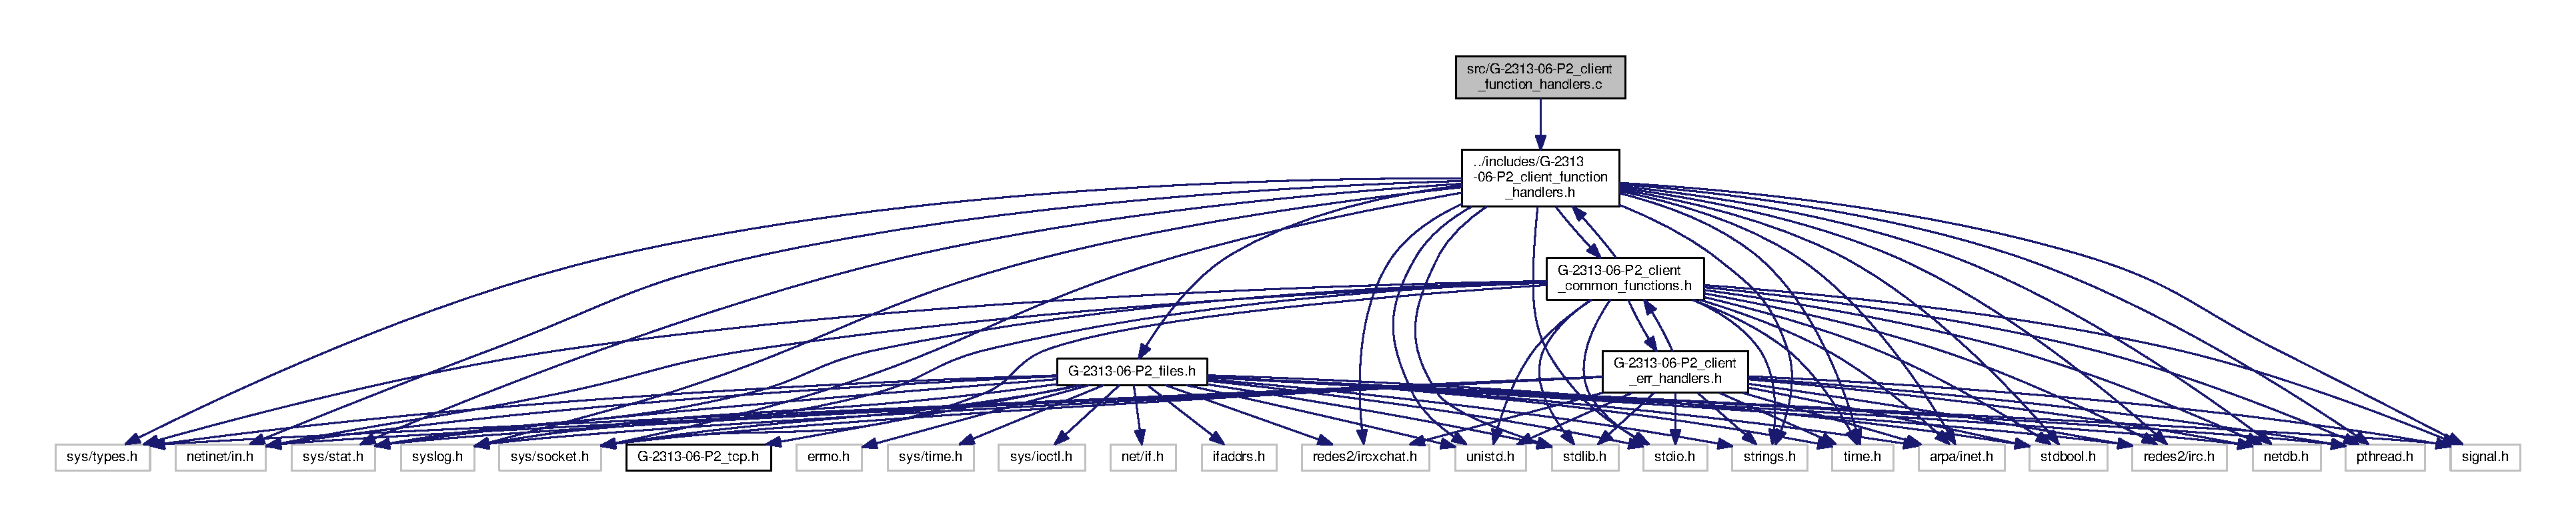
\includegraphics[width=350pt]{G-2313-06-P2__client__function__handlers_8c__incl}
\end{center}
\end{figure}
\subsection*{Funciones}
\begin{DoxyCompactItemize}
\item 
void \hyperlink{G-2313-06-P2__client__function__handlers_8c_a3271de16b2f7077059343bd6f52e4866}{server\+\_\+in\+\_\+command\+\_\+nick} (char $\ast$command)
\item 
void \hyperlink{G-2313-06-P2__client__function__handlers_8c_a64c324e32edf01774722861d3abc7be3}{server\+\_\+in\+\_\+command\+\_\+join} (char $\ast$command)
\item 
void \hyperlink{G-2313-06-P2__client__function__handlers_8c_a53568ffb9d2301140815861c2f7178ad}{server\+\_\+in\+\_\+command\+\_\+part} (char $\ast$command)
\item 
void \hyperlink{G-2313-06-P2__client__function__handlers_8c_ae5f66619469f8ea0efa0a7a5d75938dc}{server\+\_\+in\+\_\+command\+\_\+mode} (char $\ast$command)
\item 
void \hyperlink{G-2313-06-P2__client__function__handlers_8c_ad908abfd32d53b9483d5afa4ca18ff14}{server\+\_\+in\+\_\+command\+\_\+topic} (char $\ast$command)
\item 
void \hyperlink{G-2313-06-P2__client__function__handlers_8c_aa3d18c616914957b9794f086466788bb}{server\+\_\+in\+\_\+command\+\_\+kick} (char $\ast$command)
\item 
void \hyperlink{G-2313-06-P2__client__function__handlers_8c_a858c0e5586286e535590f7de14620300}{server\+\_\+in\+\_\+command\+\_\+who} (char $\ast$command)
\item 
void \hyperlink{G-2313-06-P2__client__function__handlers_8c_a32594eebe5482f63993568825a9e126a}{server\+\_\+in\+\_\+command\+\_\+privmsg} (char $\ast$command)
\item 
void \hyperlink{G-2313-06-P2__client__function__handlers_8c_a09a9d4d13037bd783036a70d5a76ac46}{server\+\_\+in\+\_\+command\+\_\+ping} (char $\ast$command)
\item 
void \hyperlink{G-2313-06-P2__client__function__handlers_8c_a06042a6459e89e0ae7586e66f8595fa3}{server\+\_\+in\+\_\+command\+\_\+pong} (char $\ast$command)
\item 
void \hyperlink{G-2313-06-P2__client__function__handlers_8c_a294ef5e5070e9859d88beb603ef950f2}{server\+\_\+in\+\_\+command\+\_\+rpl\+\_\+welcome} (char $\ast$command)
\item 
void \hyperlink{G-2313-06-P2__client__function__handlers_8c_a40e46db4017fb76fc547536d9c51f5d9}{server\+\_\+in\+\_\+command\+\_\+rpl\+\_\+created} (char $\ast$command)
\item 
void \hyperlink{G-2313-06-P2__client__function__handlers_8c_a3f4cf6c0d74b06a0916f7a9619972eee}{server\+\_\+in\+\_\+command\+\_\+rpl\+\_\+yourhost} (char $\ast$command)
\item 
void \hyperlink{G-2313-06-P2__client__function__handlers_8c_af5091cf59cbab7ce259c405c019fa8dd}{server\+\_\+in\+\_\+command\+\_\+rpl\+\_\+luserclient} (char $\ast$command)
\item 
void \hyperlink{G-2313-06-P2__client__function__handlers_8c_a5764225aa28906c7ccebf0996b2c5a08}{server\+\_\+in\+\_\+command\+\_\+rpl\+\_\+luserme} (char $\ast$command)
\item 
void \hyperlink{G-2313-06-P2__client__function__handlers_8c_acd688f18855dcb6ee9bf10a72e0c8f6c}{server\+\_\+in\+\_\+command\+\_\+rpl\+\_\+motdstart} (char $\ast$command)
\item 
void \hyperlink{G-2313-06-P2__client__function__handlers_8c_a774c98f4ea94eb6f92a5b22d33030674}{server\+\_\+in\+\_\+command\+\_\+rpl\+\_\+motd} (char $\ast$command)
\item 
void \hyperlink{G-2313-06-P2__client__function__handlers_8c_ad22233e08c30cad9e0598f80b5b38744}{server\+\_\+in\+\_\+command\+\_\+rpl\+\_\+endofmotd} (char $\ast$command)
\item 
void \hyperlink{G-2313-06-P2__client__function__handlers_8c_a86782df5d9b151dd061b9831a47a2c5f}{server\+\_\+in\+\_\+command\+\_\+rpl\+\_\+whoreply} (char $\ast$command)
\item 
void \hyperlink{G-2313-06-P2__client__function__handlers_8c_add282510a7e92a90d45091e6dc3a3488}{server\+\_\+in\+\_\+command\+\_\+rpl\+\_\+away} (char $\ast$command)
\item 
void \hyperlink{G-2313-06-P2__client__function__handlers_8c_ada377e1754f9a22a2ebe0bada8838b5b}{server\+\_\+in\+\_\+command\+\_\+rpl\+\_\+nowaway} (char $\ast$command)
\item 
void \hyperlink{G-2313-06-P2__client__function__handlers_8c_abc030e3bc9ce4ad126ea2c66e304e2d5}{server\+\_\+in\+\_\+command\+\_\+rpl\+\_\+topic} (char $\ast$command)
\item 
void \hyperlink{G-2313-06-P2__client__function__handlers_8c_ab9b55bd1e18bde61e8327fcf6936d91f}{server\+\_\+in\+\_\+command\+\_\+rpl\+\_\+notopic} (char $\ast$command)
\item 
void \hyperlink{G-2313-06-P2__client__function__handlers_8c_a24bb76a5941798964a8dd18e1cfb1d81}{server\+\_\+in\+\_\+command\+\_\+rpl\+\_\+youroper} (char $\ast$command)
\item 
void \hyperlink{G-2313-06-P2__client__function__handlers_8c_aa885b5d729d8a920a1c38678abdbe6b7}{server\+\_\+in\+\_\+command\+\_\+rpl\+\_\+luserop} (char $\ast$command)
\item 
void \hyperlink{G-2313-06-P2__client__function__handlers_8c_ae53c29cff5b1b8b3981be92c317cf29d}{server\+\_\+in\+\_\+command\+\_\+rpl\+\_\+luserchannels} (char $\ast$command)
\item 
void \hyperlink{G-2313-06-P2__client__function__handlers_8c_a9a54a1989e86596904bc4d1c2618ba84}{server\+\_\+in\+\_\+command\+\_\+rpl\+\_\+youreservice} (char $\ast$command)
\item 
void \hyperlink{G-2313-06-P2__client__function__handlers_8c_aa4c4d377b1cde9f0b40997a54c81c3de}{server\+\_\+in\+\_\+command\+\_\+rpl\+\_\+myinfo} (char $\ast$command)
\item 
void \hyperlink{G-2313-06-P2__client__function__handlers_8c_a441993de1d4be974fab21e17aacc553e}{server\+\_\+in\+\_\+command\+\_\+rpl\+\_\+endofwho} (char $\ast$command)
\item 
void \hyperlink{G-2313-06-P2__client__function__handlers_8c_a56185c77cfea8620c1ce413a44865bc4}{server\+\_\+in\+\_\+command\+\_\+rpl\+\_\+endofwhois} (char $\ast$command)
\item 
void \hyperlink{G-2313-06-P2__client__function__handlers_8c_a6477df39f199931be3274e311a18b276}{server\+\_\+in\+\_\+command\+\_\+rpl\+\_\+info} (char $\ast$command)
\item 
void \hyperlink{G-2313-06-P2__client__function__handlers_8c_af2190c9ca68abe019cde6f3a18e380c2}{server\+\_\+in\+\_\+command\+\_\+rpl\+\_\+whoisuser} (char $\ast$command)
\item 
void \hyperlink{G-2313-06-P2__client__function__handlers_8c_a7ed4d1bd7f485fe7c6d26bd1d8eef662}{server\+\_\+in\+\_\+command\+\_\+rpl\+\_\+whoischannels} (char $\ast$command)
\item 
void \hyperlink{G-2313-06-P2__client__function__handlers_8c_a890fb67530ca5c1f5c14da877fc9ba21}{server\+\_\+in\+\_\+command\+\_\+rpl\+\_\+whoisoperator} (char $\ast$command)
\item 
void \hyperlink{G-2313-06-P2__client__function__handlers_8c_a27bc970f66b7e5a2f3806853c3fa156f}{server\+\_\+in\+\_\+command\+\_\+rpl\+\_\+whoisserver} (char $\ast$command)
\item 
void \hyperlink{G-2313-06-P2__client__function__handlers_8c_ada14de5a081899ca2b5eccbfb9779d62}{server\+\_\+in\+\_\+command\+\_\+rpl\+\_\+whoisidle} (char $\ast$command)
\item 
void \hyperlink{G-2313-06-P2__client__function__handlers_8c_a23ae57a558e401f83bc03209efb34be2}{server\+\_\+in\+\_\+command\+\_\+rpl\+\_\+channelmodeis} (char $\ast$command)
\item 
void \hyperlink{G-2313-06-P2__client__function__handlers_8c_a11fdd753a098bb69dc7ca93a89433abb}{server\+\_\+in\+\_\+command\+\_\+rpl\+\_\+endofnames} (char $\ast$command)
\item 
void \hyperlink{G-2313-06-P2__client__function__handlers_8c_a032cc47903f14a4fbdcec9e54f6a8e4a}{server\+\_\+in\+\_\+command\+\_\+rpl\+\_\+list} (char $\ast$command)
\item 
void \hyperlink{G-2313-06-P2__client__function__handlers_8c_ad4a1e3d492ae6907a5e15e92cb9b69f7}{server\+\_\+in\+\_\+command\+\_\+rpl\+\_\+listend} (char $\ast$command)
\item 
void \hyperlink{G-2313-06-P2__client__function__handlers_8c_a770ed57ba6c48c4a349208439e3f19ef}{server\+\_\+in\+\_\+command\+\_\+rpl\+\_\+namreply} (char $\ast$command)
\item 
void \hyperlink{G-2313-06-P2__client__function__handlers_8c_a43f3e63fcf23bd087e02911f79b789b0}{server\+\_\+out\+\_\+command\+\_\+nick} (char $\ast$command)
\item 
void \hyperlink{G-2313-06-P2__client__function__handlers_8c_a49e60d29aef3725ab2a91c7f99e61021}{server\+\_\+out\+\_\+command\+\_\+join} (char $\ast$command)
\item 
void \hyperlink{G-2313-06-P2__client__function__handlers_8c_ab2f3bd779063c27074a6cdce0f98ee0a}{server\+\_\+out\+\_\+command\+\_\+names} (char $\ast$command)
\item 
void \hyperlink{G-2313-06-P2__client__function__handlers_8c_a0a66dad6908cd303ae31f06dda298e5f}{server\+\_\+out\+\_\+command\+\_\+list} (char $\ast$command)
\item 
void \hyperlink{G-2313-06-P2__client__function__handlers_8c_a39f81214b8394e2b7fb0989e5fe10fb3}{server\+\_\+out\+\_\+command\+\_\+part} (char $\ast$command)
\item 
void \hyperlink{G-2313-06-P2__client__function__handlers_8c_afa583197101ff2eb07ab93ccd10da962}{server\+\_\+out\+\_\+command\+\_\+mode} (char $\ast$command)
\item 
void \hyperlink{G-2313-06-P2__client__function__handlers_8c_a4e94d9864089e10109fc24ce92d4368b}{server\+\_\+out\+\_\+command\+\_\+kick} (char $\ast$command)
\item 
void \hyperlink{G-2313-06-P2__client__function__handlers_8c_a4c442d20949a3a3e84551a5f23ce8263}{server\+\_\+out\+\_\+command\+\_\+privmsg} (char $\ast$command)
\item 
void \hyperlink{G-2313-06-P2__client__function__handlers_8c_af34c02fb3b13802e2c457a302c66cb89}{server\+\_\+out\+\_\+command\+\_\+whois} (char $\ast$command)
\item 
void \hyperlink{G-2313-06-P2__client__function__handlers_8c_a6760491bb5560bf6db1e652022f0720f}{server\+\_\+out\+\_\+command\+\_\+invite} (char $\ast$command)
\item 
void \hyperlink{G-2313-06-P2__client__function__handlers_8c_affd97f456e87778153ec551468bb7f25}{server\+\_\+out\+\_\+command\+\_\+topic} (char $\ast$command)
\item 
void \hyperlink{G-2313-06-P2__client__function__handlers_8c_a9680c711ecaa492727c14a9c5d7e82ca}{server\+\_\+out\+\_\+command\+\_\+me} (char $\ast$command)
\item 
void \hyperlink{G-2313-06-P2__client__function__handlers_8c_ad2280719361affeaf8d3a663b48f0b3f}{server\+\_\+out\+\_\+command\+\_\+msg} (char $\ast$command)
\item 
void \hyperlink{G-2313-06-P2__client__function__handlers_8c_a6e05dad9592e0e473e84647cfe263034}{server\+\_\+out\+\_\+command\+\_\+notice} (char $\ast$command)
\item 
void \hyperlink{G-2313-06-P2__client__function__handlers_8c_a3b0bef634e60a6e59223cfb7e444fb36}{server\+\_\+out\+\_\+command\+\_\+ignore} (char $\ast$command)
\item 
void \hyperlink{G-2313-06-P2__client__function__handlers_8c_a4f8f2db21b7edd9e6b7fbad232ee27fd}{server\+\_\+out\+\_\+command\+\_\+who} (char $\ast$command)
\item 
void \hyperlink{G-2313-06-P2__client__function__handlers_8c_a74f475c007446256a2cbada71f51f30a}{server\+\_\+out\+\_\+command\+\_\+whowas} (char $\ast$command)
\item 
void \hyperlink{G-2313-06-P2__client__function__handlers_8c_ae721ae6a65ec5f0790d6b6883dcf94a5}{server\+\_\+out\+\_\+command\+\_\+motd} (char $\ast$command)
\item 
void \hyperlink{G-2313-06-P2__client__function__handlers_8c_ac0c8a1e0d4144fd3d78c124bad9228d6}{server\+\_\+out\+\_\+command\+\_\+away} (char $\ast$command)
\item 
void \hyperlink{G-2313-06-P2__client__function__handlers_8c_a3719651e6671245a46f4994fcf462c7d}{server\+\_\+out\+\_\+command\+\_\+ping} (char $\ast$command)
\end{DoxyCompactItemize}
\subsection*{Variables}
\begin{DoxyCompactItemize}
\item 
int \hyperlink{G-2313-06-P2__client__function__handlers_8c_adeadf7cb6916a10c7142ce7d265ab32a}{socket\+\_\+desc}
\item 
char $\ast$ \hyperlink{G-2313-06-P2__client__function__handlers_8c_ab93a317ee9a27c82844c9128a76b136a}{nick\+\_\+cliente}
\end{DoxyCompactItemize}


\subsection{Documentación de las funciones}
\index{G-\/2313-\/06-\/\+P2\+\_\+client\+\_\+function\+\_\+handlers.\+c@{G-\/2313-\/06-\/\+P2\+\_\+client\+\_\+function\+\_\+handlers.\+c}!server\+\_\+in\+\_\+command\+\_\+join@{server\+\_\+in\+\_\+command\+\_\+join}}
\index{server\+\_\+in\+\_\+command\+\_\+join@{server\+\_\+in\+\_\+command\+\_\+join}!G-\/2313-\/06-\/\+P2\+\_\+client\+\_\+function\+\_\+handlers.\+c@{G-\/2313-\/06-\/\+P2\+\_\+client\+\_\+function\+\_\+handlers.\+c}}
\subsubsection[{\texorpdfstring{server\+\_\+in\+\_\+command\+\_\+join(char $\ast$command)}{server_in_command_join(char *command)}}]{\setlength{\rightskip}{0pt plus 5cm}void server\+\_\+in\+\_\+command\+\_\+join (
\begin{DoxyParamCaption}
\item[{char $\ast$}]{command}
\end{DoxyParamCaption}
)}\hypertarget{G-2313-06-P2__client__function__handlers_8c_a64c324e32edf01774722861d3abc7be3}{}\label{G-2313-06-P2__client__function__handlers_8c_a64c324e32edf01774722861d3abc7be3}


Definición en la línea 51 del archivo G-\/2313-\/06-\/\+P2\+\_\+client\+\_\+function\+\_\+handlers.\+c.

\index{G-\/2313-\/06-\/\+P2\+\_\+client\+\_\+function\+\_\+handlers.\+c@{G-\/2313-\/06-\/\+P2\+\_\+client\+\_\+function\+\_\+handlers.\+c}!server\+\_\+in\+\_\+command\+\_\+kick@{server\+\_\+in\+\_\+command\+\_\+kick}}
\index{server\+\_\+in\+\_\+command\+\_\+kick@{server\+\_\+in\+\_\+command\+\_\+kick}!G-\/2313-\/06-\/\+P2\+\_\+client\+\_\+function\+\_\+handlers.\+c@{G-\/2313-\/06-\/\+P2\+\_\+client\+\_\+function\+\_\+handlers.\+c}}
\subsubsection[{\texorpdfstring{server\+\_\+in\+\_\+command\+\_\+kick(char $\ast$command)}{server_in_command_kick(char *command)}}]{\setlength{\rightskip}{0pt plus 5cm}void server\+\_\+in\+\_\+command\+\_\+kick (
\begin{DoxyParamCaption}
\item[{char $\ast$}]{command}
\end{DoxyParamCaption}
)}\hypertarget{G-2313-06-P2__client__function__handlers_8c_aa3d18c616914957b9794f086466788bb}{}\label{G-2313-06-P2__client__function__handlers_8c_aa3d18c616914957b9794f086466788bb}


Definición en la línea 204 del archivo G-\/2313-\/06-\/\+P2\+\_\+client\+\_\+function\+\_\+handlers.\+c.

\index{G-\/2313-\/06-\/\+P2\+\_\+client\+\_\+function\+\_\+handlers.\+c@{G-\/2313-\/06-\/\+P2\+\_\+client\+\_\+function\+\_\+handlers.\+c}!server\+\_\+in\+\_\+command\+\_\+mode@{server\+\_\+in\+\_\+command\+\_\+mode}}
\index{server\+\_\+in\+\_\+command\+\_\+mode@{server\+\_\+in\+\_\+command\+\_\+mode}!G-\/2313-\/06-\/\+P2\+\_\+client\+\_\+function\+\_\+handlers.\+c@{G-\/2313-\/06-\/\+P2\+\_\+client\+\_\+function\+\_\+handlers.\+c}}
\subsubsection[{\texorpdfstring{server\+\_\+in\+\_\+command\+\_\+mode(char $\ast$command)}{server_in_command_mode(char *command)}}]{\setlength{\rightskip}{0pt plus 5cm}void server\+\_\+in\+\_\+command\+\_\+mode (
\begin{DoxyParamCaption}
\item[{char $\ast$}]{command}
\end{DoxyParamCaption}
)}\hypertarget{G-2313-06-P2__client__function__handlers_8c_ae5f66619469f8ea0efa0a7a5d75938dc}{}\label{G-2313-06-P2__client__function__handlers_8c_ae5f66619469f8ea0efa0a7a5d75938dc}


Definición en la línea 103 del archivo G-\/2313-\/06-\/\+P2\+\_\+client\+\_\+function\+\_\+handlers.\+c.

\index{G-\/2313-\/06-\/\+P2\+\_\+client\+\_\+function\+\_\+handlers.\+c@{G-\/2313-\/06-\/\+P2\+\_\+client\+\_\+function\+\_\+handlers.\+c}!server\+\_\+in\+\_\+command\+\_\+nick@{server\+\_\+in\+\_\+command\+\_\+nick}}
\index{server\+\_\+in\+\_\+command\+\_\+nick@{server\+\_\+in\+\_\+command\+\_\+nick}!G-\/2313-\/06-\/\+P2\+\_\+client\+\_\+function\+\_\+handlers.\+c@{G-\/2313-\/06-\/\+P2\+\_\+client\+\_\+function\+\_\+handlers.\+c}}
\subsubsection[{\texorpdfstring{server\+\_\+in\+\_\+command\+\_\+nick(char $\ast$command)}{server_in_command_nick(char *command)}}]{\setlength{\rightskip}{0pt plus 5cm}void server\+\_\+in\+\_\+command\+\_\+nick (
\begin{DoxyParamCaption}
\item[{char $\ast$}]{command}
\end{DoxyParamCaption}
)}\hypertarget{G-2313-06-P2__client__function__handlers_8c_a3271de16b2f7077059343bd6f52e4866}{}\label{G-2313-06-P2__client__function__handlers_8c_a3271de16b2f7077059343bd6f52e4866}


Definición en la línea 7 del archivo G-\/2313-\/06-\/\+P2\+\_\+client\+\_\+function\+\_\+handlers.\+c.

\index{G-\/2313-\/06-\/\+P2\+\_\+client\+\_\+function\+\_\+handlers.\+c@{G-\/2313-\/06-\/\+P2\+\_\+client\+\_\+function\+\_\+handlers.\+c}!server\+\_\+in\+\_\+command\+\_\+part@{server\+\_\+in\+\_\+command\+\_\+part}}
\index{server\+\_\+in\+\_\+command\+\_\+part@{server\+\_\+in\+\_\+command\+\_\+part}!G-\/2313-\/06-\/\+P2\+\_\+client\+\_\+function\+\_\+handlers.\+c@{G-\/2313-\/06-\/\+P2\+\_\+client\+\_\+function\+\_\+handlers.\+c}}
\subsubsection[{\texorpdfstring{server\+\_\+in\+\_\+command\+\_\+part(char $\ast$command)}{server_in_command_part(char *command)}}]{\setlength{\rightskip}{0pt plus 5cm}void server\+\_\+in\+\_\+command\+\_\+part (
\begin{DoxyParamCaption}
\item[{char $\ast$}]{command}
\end{DoxyParamCaption}
)}\hypertarget{G-2313-06-P2__client__function__handlers_8c_a53568ffb9d2301140815861c2f7178ad}{}\label{G-2313-06-P2__client__function__handlers_8c_a53568ffb9d2301140815861c2f7178ad}


Definición en la línea 83 del archivo G-\/2313-\/06-\/\+P2\+\_\+client\+\_\+function\+\_\+handlers.\+c.

\index{G-\/2313-\/06-\/\+P2\+\_\+client\+\_\+function\+\_\+handlers.\+c@{G-\/2313-\/06-\/\+P2\+\_\+client\+\_\+function\+\_\+handlers.\+c}!server\+\_\+in\+\_\+command\+\_\+ping@{server\+\_\+in\+\_\+command\+\_\+ping}}
\index{server\+\_\+in\+\_\+command\+\_\+ping@{server\+\_\+in\+\_\+command\+\_\+ping}!G-\/2313-\/06-\/\+P2\+\_\+client\+\_\+function\+\_\+handlers.\+c@{G-\/2313-\/06-\/\+P2\+\_\+client\+\_\+function\+\_\+handlers.\+c}}
\subsubsection[{\texorpdfstring{server\+\_\+in\+\_\+command\+\_\+ping(char $\ast$command)}{server_in_command_ping(char *command)}}]{\setlength{\rightskip}{0pt plus 5cm}void server\+\_\+in\+\_\+command\+\_\+ping (
\begin{DoxyParamCaption}
\item[{char $\ast$}]{command}
\end{DoxyParamCaption}
)}\hypertarget{G-2313-06-P2__client__function__handlers_8c_a09a9d4d13037bd783036a70d5a76ac46}{}\label{G-2313-06-P2__client__function__handlers_8c_a09a9d4d13037bd783036a70d5a76ac46}


Definición en la línea 274 del archivo G-\/2313-\/06-\/\+P2\+\_\+client\+\_\+function\+\_\+handlers.\+c.

\index{G-\/2313-\/06-\/\+P2\+\_\+client\+\_\+function\+\_\+handlers.\+c@{G-\/2313-\/06-\/\+P2\+\_\+client\+\_\+function\+\_\+handlers.\+c}!server\+\_\+in\+\_\+command\+\_\+pong@{server\+\_\+in\+\_\+command\+\_\+pong}}
\index{server\+\_\+in\+\_\+command\+\_\+pong@{server\+\_\+in\+\_\+command\+\_\+pong}!G-\/2313-\/06-\/\+P2\+\_\+client\+\_\+function\+\_\+handlers.\+c@{G-\/2313-\/06-\/\+P2\+\_\+client\+\_\+function\+\_\+handlers.\+c}}
\subsubsection[{\texorpdfstring{server\+\_\+in\+\_\+command\+\_\+pong(char $\ast$command)}{server_in_command_pong(char *command)}}]{\setlength{\rightskip}{0pt plus 5cm}void server\+\_\+in\+\_\+command\+\_\+pong (
\begin{DoxyParamCaption}
\item[{char $\ast$}]{command}
\end{DoxyParamCaption}
)}\hypertarget{G-2313-06-P2__client__function__handlers_8c_a06042a6459e89e0ae7586e66f8595fa3}{}\label{G-2313-06-P2__client__function__handlers_8c_a06042a6459e89e0ae7586e66f8595fa3}


Definición en la línea 289 del archivo G-\/2313-\/06-\/\+P2\+\_\+client\+\_\+function\+\_\+handlers.\+c.

\index{G-\/2313-\/06-\/\+P2\+\_\+client\+\_\+function\+\_\+handlers.\+c@{G-\/2313-\/06-\/\+P2\+\_\+client\+\_\+function\+\_\+handlers.\+c}!server\+\_\+in\+\_\+command\+\_\+privmsg@{server\+\_\+in\+\_\+command\+\_\+privmsg}}
\index{server\+\_\+in\+\_\+command\+\_\+privmsg@{server\+\_\+in\+\_\+command\+\_\+privmsg}!G-\/2313-\/06-\/\+P2\+\_\+client\+\_\+function\+\_\+handlers.\+c@{G-\/2313-\/06-\/\+P2\+\_\+client\+\_\+function\+\_\+handlers.\+c}}
\subsubsection[{\texorpdfstring{server\+\_\+in\+\_\+command\+\_\+privmsg(char $\ast$command)}{server_in_command_privmsg(char *command)}}]{\setlength{\rightskip}{0pt plus 5cm}void server\+\_\+in\+\_\+command\+\_\+privmsg (
\begin{DoxyParamCaption}
\item[{char $\ast$}]{command}
\end{DoxyParamCaption}
)}\hypertarget{G-2313-06-P2__client__function__handlers_8c_a32594eebe5482f63993568825a9e126a}{}\label{G-2313-06-P2__client__function__handlers_8c_a32594eebe5482f63993568825a9e126a}


Definición en la línea 241 del archivo G-\/2313-\/06-\/\+P2\+\_\+client\+\_\+function\+\_\+handlers.\+c.

\index{G-\/2313-\/06-\/\+P2\+\_\+client\+\_\+function\+\_\+handlers.\+c@{G-\/2313-\/06-\/\+P2\+\_\+client\+\_\+function\+\_\+handlers.\+c}!server\+\_\+in\+\_\+command\+\_\+rpl\+\_\+away@{server\+\_\+in\+\_\+command\+\_\+rpl\+\_\+away}}
\index{server\+\_\+in\+\_\+command\+\_\+rpl\+\_\+away@{server\+\_\+in\+\_\+command\+\_\+rpl\+\_\+away}!G-\/2313-\/06-\/\+P2\+\_\+client\+\_\+function\+\_\+handlers.\+c@{G-\/2313-\/06-\/\+P2\+\_\+client\+\_\+function\+\_\+handlers.\+c}}
\subsubsection[{\texorpdfstring{server\+\_\+in\+\_\+command\+\_\+rpl\+\_\+away(char $\ast$command)}{server_in_command_rpl_away(char *command)}}]{\setlength{\rightskip}{0pt plus 5cm}void server\+\_\+in\+\_\+command\+\_\+rpl\+\_\+away (
\begin{DoxyParamCaption}
\item[{char $\ast$}]{command}
\end{DoxyParamCaption}
)}\hypertarget{G-2313-06-P2__client__function__handlers_8c_add282510a7e92a90d45091e6dc3a3488}{}\label{G-2313-06-P2__client__function__handlers_8c_add282510a7e92a90d45091e6dc3a3488}


Definición en la línea 410 del archivo G-\/2313-\/06-\/\+P2\+\_\+client\+\_\+function\+\_\+handlers.\+c.

\index{G-\/2313-\/06-\/\+P2\+\_\+client\+\_\+function\+\_\+handlers.\+c@{G-\/2313-\/06-\/\+P2\+\_\+client\+\_\+function\+\_\+handlers.\+c}!server\+\_\+in\+\_\+command\+\_\+rpl\+\_\+channelmodeis@{server\+\_\+in\+\_\+command\+\_\+rpl\+\_\+channelmodeis}}
\index{server\+\_\+in\+\_\+command\+\_\+rpl\+\_\+channelmodeis@{server\+\_\+in\+\_\+command\+\_\+rpl\+\_\+channelmodeis}!G-\/2313-\/06-\/\+P2\+\_\+client\+\_\+function\+\_\+handlers.\+c@{G-\/2313-\/06-\/\+P2\+\_\+client\+\_\+function\+\_\+handlers.\+c}}
\subsubsection[{\texorpdfstring{server\+\_\+in\+\_\+command\+\_\+rpl\+\_\+channelmodeis(char $\ast$command)}{server_in_command_rpl_channelmodeis(char *command)}}]{\setlength{\rightskip}{0pt plus 5cm}void server\+\_\+in\+\_\+command\+\_\+rpl\+\_\+channelmodeis (
\begin{DoxyParamCaption}
\item[{char $\ast$}]{command}
\end{DoxyParamCaption}
)}\hypertarget{G-2313-06-P2__client__function__handlers_8c_a23ae57a558e401f83bc03209efb34be2}{}\label{G-2313-06-P2__client__function__handlers_8c_a23ae57a558e401f83bc03209efb34be2}


Definición en la línea 602 del archivo G-\/2313-\/06-\/\+P2\+\_\+client\+\_\+function\+\_\+handlers.\+c.

\index{G-\/2313-\/06-\/\+P2\+\_\+client\+\_\+function\+\_\+handlers.\+c@{G-\/2313-\/06-\/\+P2\+\_\+client\+\_\+function\+\_\+handlers.\+c}!server\+\_\+in\+\_\+command\+\_\+rpl\+\_\+created@{server\+\_\+in\+\_\+command\+\_\+rpl\+\_\+created}}
\index{server\+\_\+in\+\_\+command\+\_\+rpl\+\_\+created@{server\+\_\+in\+\_\+command\+\_\+rpl\+\_\+created}!G-\/2313-\/06-\/\+P2\+\_\+client\+\_\+function\+\_\+handlers.\+c@{G-\/2313-\/06-\/\+P2\+\_\+client\+\_\+function\+\_\+handlers.\+c}}
\subsubsection[{\texorpdfstring{server\+\_\+in\+\_\+command\+\_\+rpl\+\_\+created(char $\ast$command)}{server_in_command_rpl_created(char *command)}}]{\setlength{\rightskip}{0pt plus 5cm}void server\+\_\+in\+\_\+command\+\_\+rpl\+\_\+created (
\begin{DoxyParamCaption}
\item[{char $\ast$}]{command}
\end{DoxyParamCaption}
)}\hypertarget{G-2313-06-P2__client__function__handlers_8c_a40e46db4017fb76fc547536d9c51f5d9}{}\label{G-2313-06-P2__client__function__handlers_8c_a40e46db4017fb76fc547536d9c51f5d9}


Definición en la línea 318 del archivo G-\/2313-\/06-\/\+P2\+\_\+client\+\_\+function\+\_\+handlers.\+c.

\index{G-\/2313-\/06-\/\+P2\+\_\+client\+\_\+function\+\_\+handlers.\+c@{G-\/2313-\/06-\/\+P2\+\_\+client\+\_\+function\+\_\+handlers.\+c}!server\+\_\+in\+\_\+command\+\_\+rpl\+\_\+endofmotd@{server\+\_\+in\+\_\+command\+\_\+rpl\+\_\+endofmotd}}
\index{server\+\_\+in\+\_\+command\+\_\+rpl\+\_\+endofmotd@{server\+\_\+in\+\_\+command\+\_\+rpl\+\_\+endofmotd}!G-\/2313-\/06-\/\+P2\+\_\+client\+\_\+function\+\_\+handlers.\+c@{G-\/2313-\/06-\/\+P2\+\_\+client\+\_\+function\+\_\+handlers.\+c}}
\subsubsection[{\texorpdfstring{server\+\_\+in\+\_\+command\+\_\+rpl\+\_\+endofmotd(char $\ast$command)}{server_in_command_rpl_endofmotd(char *command)}}]{\setlength{\rightskip}{0pt plus 5cm}void server\+\_\+in\+\_\+command\+\_\+rpl\+\_\+endofmotd (
\begin{DoxyParamCaption}
\item[{char $\ast$}]{command}
\end{DoxyParamCaption}
)}\hypertarget{G-2313-06-P2__client__function__handlers_8c_ad22233e08c30cad9e0598f80b5b38744}{}\label{G-2313-06-P2__client__function__handlers_8c_ad22233e08c30cad9e0598f80b5b38744}


Definición en la línea 374 del archivo G-\/2313-\/06-\/\+P2\+\_\+client\+\_\+function\+\_\+handlers.\+c.

\index{G-\/2313-\/06-\/\+P2\+\_\+client\+\_\+function\+\_\+handlers.\+c@{G-\/2313-\/06-\/\+P2\+\_\+client\+\_\+function\+\_\+handlers.\+c}!server\+\_\+in\+\_\+command\+\_\+rpl\+\_\+endofnames@{server\+\_\+in\+\_\+command\+\_\+rpl\+\_\+endofnames}}
\index{server\+\_\+in\+\_\+command\+\_\+rpl\+\_\+endofnames@{server\+\_\+in\+\_\+command\+\_\+rpl\+\_\+endofnames}!G-\/2313-\/06-\/\+P2\+\_\+client\+\_\+function\+\_\+handlers.\+c@{G-\/2313-\/06-\/\+P2\+\_\+client\+\_\+function\+\_\+handlers.\+c}}
\subsubsection[{\texorpdfstring{server\+\_\+in\+\_\+command\+\_\+rpl\+\_\+endofnames(char $\ast$command)}{server_in_command_rpl_endofnames(char *command)}}]{\setlength{\rightskip}{0pt plus 5cm}void server\+\_\+in\+\_\+command\+\_\+rpl\+\_\+endofnames (
\begin{DoxyParamCaption}
\item[{char $\ast$}]{command}
\end{DoxyParamCaption}
)}\hypertarget{G-2313-06-P2__client__function__handlers_8c_a11fdd753a098bb69dc7ca93a89433abb}{}\label{G-2313-06-P2__client__function__handlers_8c_a11fdd753a098bb69dc7ca93a89433abb}


Definición en la línea 613 del archivo G-\/2313-\/06-\/\+P2\+\_\+client\+\_\+function\+\_\+handlers.\+c.

\index{G-\/2313-\/06-\/\+P2\+\_\+client\+\_\+function\+\_\+handlers.\+c@{G-\/2313-\/06-\/\+P2\+\_\+client\+\_\+function\+\_\+handlers.\+c}!server\+\_\+in\+\_\+command\+\_\+rpl\+\_\+endofwho@{server\+\_\+in\+\_\+command\+\_\+rpl\+\_\+endofwho}}
\index{server\+\_\+in\+\_\+command\+\_\+rpl\+\_\+endofwho@{server\+\_\+in\+\_\+command\+\_\+rpl\+\_\+endofwho}!G-\/2313-\/06-\/\+P2\+\_\+client\+\_\+function\+\_\+handlers.\+c@{G-\/2313-\/06-\/\+P2\+\_\+client\+\_\+function\+\_\+handlers.\+c}}
\subsubsection[{\texorpdfstring{server\+\_\+in\+\_\+command\+\_\+rpl\+\_\+endofwho(char $\ast$command)}{server_in_command_rpl_endofwho(char *command)}}]{\setlength{\rightskip}{0pt plus 5cm}void server\+\_\+in\+\_\+command\+\_\+rpl\+\_\+endofwho (
\begin{DoxyParamCaption}
\item[{char $\ast$}]{command}
\end{DoxyParamCaption}
)}\hypertarget{G-2313-06-P2__client__function__handlers_8c_a441993de1d4be974fab21e17aacc553e}{}\label{G-2313-06-P2__client__function__handlers_8c_a441993de1d4be974fab21e17aacc553e}


Definición en la línea 515 del archivo G-\/2313-\/06-\/\+P2\+\_\+client\+\_\+function\+\_\+handlers.\+c.

\index{G-\/2313-\/06-\/\+P2\+\_\+client\+\_\+function\+\_\+handlers.\+c@{G-\/2313-\/06-\/\+P2\+\_\+client\+\_\+function\+\_\+handlers.\+c}!server\+\_\+in\+\_\+command\+\_\+rpl\+\_\+endofwhois@{server\+\_\+in\+\_\+command\+\_\+rpl\+\_\+endofwhois}}
\index{server\+\_\+in\+\_\+command\+\_\+rpl\+\_\+endofwhois@{server\+\_\+in\+\_\+command\+\_\+rpl\+\_\+endofwhois}!G-\/2313-\/06-\/\+P2\+\_\+client\+\_\+function\+\_\+handlers.\+c@{G-\/2313-\/06-\/\+P2\+\_\+client\+\_\+function\+\_\+handlers.\+c}}
\subsubsection[{\texorpdfstring{server\+\_\+in\+\_\+command\+\_\+rpl\+\_\+endofwhois(char $\ast$command)}{server_in_command_rpl_endofwhois(char *command)}}]{\setlength{\rightskip}{0pt plus 5cm}void server\+\_\+in\+\_\+command\+\_\+rpl\+\_\+endofwhois (
\begin{DoxyParamCaption}
\item[{char $\ast$}]{command}
\end{DoxyParamCaption}
)}\hypertarget{G-2313-06-P2__client__function__handlers_8c_a56185c77cfea8620c1ce413a44865bc4}{}\label{G-2313-06-P2__client__function__handlers_8c_a56185c77cfea8620c1ce413a44865bc4}


Definición en la línea 524 del archivo G-\/2313-\/06-\/\+P2\+\_\+client\+\_\+function\+\_\+handlers.\+c.

\index{G-\/2313-\/06-\/\+P2\+\_\+client\+\_\+function\+\_\+handlers.\+c@{G-\/2313-\/06-\/\+P2\+\_\+client\+\_\+function\+\_\+handlers.\+c}!server\+\_\+in\+\_\+command\+\_\+rpl\+\_\+info@{server\+\_\+in\+\_\+command\+\_\+rpl\+\_\+info}}
\index{server\+\_\+in\+\_\+command\+\_\+rpl\+\_\+info@{server\+\_\+in\+\_\+command\+\_\+rpl\+\_\+info}!G-\/2313-\/06-\/\+P2\+\_\+client\+\_\+function\+\_\+handlers.\+c@{G-\/2313-\/06-\/\+P2\+\_\+client\+\_\+function\+\_\+handlers.\+c}}
\subsubsection[{\texorpdfstring{server\+\_\+in\+\_\+command\+\_\+rpl\+\_\+info(char $\ast$command)}{server_in_command_rpl_info(char *command)}}]{\setlength{\rightskip}{0pt plus 5cm}void server\+\_\+in\+\_\+command\+\_\+rpl\+\_\+info (
\begin{DoxyParamCaption}
\item[{char $\ast$}]{command}
\end{DoxyParamCaption}
)}\hypertarget{G-2313-06-P2__client__function__handlers_8c_a6477df39f199931be3274e311a18b276}{}\label{G-2313-06-P2__client__function__handlers_8c_a6477df39f199931be3274e311a18b276}


Definición en la línea 533 del archivo G-\/2313-\/06-\/\+P2\+\_\+client\+\_\+function\+\_\+handlers.\+c.

\index{G-\/2313-\/06-\/\+P2\+\_\+client\+\_\+function\+\_\+handlers.\+c@{G-\/2313-\/06-\/\+P2\+\_\+client\+\_\+function\+\_\+handlers.\+c}!server\+\_\+in\+\_\+command\+\_\+rpl\+\_\+list@{server\+\_\+in\+\_\+command\+\_\+rpl\+\_\+list}}
\index{server\+\_\+in\+\_\+command\+\_\+rpl\+\_\+list@{server\+\_\+in\+\_\+command\+\_\+rpl\+\_\+list}!G-\/2313-\/06-\/\+P2\+\_\+client\+\_\+function\+\_\+handlers.\+c@{G-\/2313-\/06-\/\+P2\+\_\+client\+\_\+function\+\_\+handlers.\+c}}
\subsubsection[{\texorpdfstring{server\+\_\+in\+\_\+command\+\_\+rpl\+\_\+list(char $\ast$command)}{server_in_command_rpl_list(char *command)}}]{\setlength{\rightskip}{0pt plus 5cm}void server\+\_\+in\+\_\+command\+\_\+rpl\+\_\+list (
\begin{DoxyParamCaption}
\item[{char $\ast$}]{command}
\end{DoxyParamCaption}
)}\hypertarget{G-2313-06-P2__client__function__handlers_8c_a032cc47903f14a4fbdcec9e54f6a8e4a}{}\label{G-2313-06-P2__client__function__handlers_8c_a032cc47903f14a4fbdcec9e54f6a8e4a}


Definición en la línea 622 del archivo G-\/2313-\/06-\/\+P2\+\_\+client\+\_\+function\+\_\+handlers.\+c.

\index{G-\/2313-\/06-\/\+P2\+\_\+client\+\_\+function\+\_\+handlers.\+c@{G-\/2313-\/06-\/\+P2\+\_\+client\+\_\+function\+\_\+handlers.\+c}!server\+\_\+in\+\_\+command\+\_\+rpl\+\_\+listend@{server\+\_\+in\+\_\+command\+\_\+rpl\+\_\+listend}}
\index{server\+\_\+in\+\_\+command\+\_\+rpl\+\_\+listend@{server\+\_\+in\+\_\+command\+\_\+rpl\+\_\+listend}!G-\/2313-\/06-\/\+P2\+\_\+client\+\_\+function\+\_\+handlers.\+c@{G-\/2313-\/06-\/\+P2\+\_\+client\+\_\+function\+\_\+handlers.\+c}}
\subsubsection[{\texorpdfstring{server\+\_\+in\+\_\+command\+\_\+rpl\+\_\+listend(char $\ast$command)}{server_in_command_rpl_listend(char *command)}}]{\setlength{\rightskip}{0pt plus 5cm}void server\+\_\+in\+\_\+command\+\_\+rpl\+\_\+listend (
\begin{DoxyParamCaption}
\item[{char $\ast$}]{command}
\end{DoxyParamCaption}
)}\hypertarget{G-2313-06-P2__client__function__handlers_8c_ad4a1e3d492ae6907a5e15e92cb9b69f7}{}\label{G-2313-06-P2__client__function__handlers_8c_ad4a1e3d492ae6907a5e15e92cb9b69f7}


Definición en la línea 633 del archivo G-\/2313-\/06-\/\+P2\+\_\+client\+\_\+function\+\_\+handlers.\+c.

\index{G-\/2313-\/06-\/\+P2\+\_\+client\+\_\+function\+\_\+handlers.\+c@{G-\/2313-\/06-\/\+P2\+\_\+client\+\_\+function\+\_\+handlers.\+c}!server\+\_\+in\+\_\+command\+\_\+rpl\+\_\+luserchannels@{server\+\_\+in\+\_\+command\+\_\+rpl\+\_\+luserchannels}}
\index{server\+\_\+in\+\_\+command\+\_\+rpl\+\_\+luserchannels@{server\+\_\+in\+\_\+command\+\_\+rpl\+\_\+luserchannels}!G-\/2313-\/06-\/\+P2\+\_\+client\+\_\+function\+\_\+handlers.\+c@{G-\/2313-\/06-\/\+P2\+\_\+client\+\_\+function\+\_\+handlers.\+c}}
\subsubsection[{\texorpdfstring{server\+\_\+in\+\_\+command\+\_\+rpl\+\_\+luserchannels(char $\ast$command)}{server_in_command_rpl_luserchannels(char *command)}}]{\setlength{\rightskip}{0pt plus 5cm}void server\+\_\+in\+\_\+command\+\_\+rpl\+\_\+luserchannels (
\begin{DoxyParamCaption}
\item[{char $\ast$}]{command}
\end{DoxyParamCaption}
)}\hypertarget{G-2313-06-P2__client__function__handlers_8c_ae53c29cff5b1b8b3981be92c317cf29d}{}\label{G-2313-06-P2__client__function__handlers_8c_ae53c29cff5b1b8b3981be92c317cf29d}


Definición en la línea 479 del archivo G-\/2313-\/06-\/\+P2\+\_\+client\+\_\+function\+\_\+handlers.\+c.

\index{G-\/2313-\/06-\/\+P2\+\_\+client\+\_\+function\+\_\+handlers.\+c@{G-\/2313-\/06-\/\+P2\+\_\+client\+\_\+function\+\_\+handlers.\+c}!server\+\_\+in\+\_\+command\+\_\+rpl\+\_\+luserclient@{server\+\_\+in\+\_\+command\+\_\+rpl\+\_\+luserclient}}
\index{server\+\_\+in\+\_\+command\+\_\+rpl\+\_\+luserclient@{server\+\_\+in\+\_\+command\+\_\+rpl\+\_\+luserclient}!G-\/2313-\/06-\/\+P2\+\_\+client\+\_\+function\+\_\+handlers.\+c@{G-\/2313-\/06-\/\+P2\+\_\+client\+\_\+function\+\_\+handlers.\+c}}
\subsubsection[{\texorpdfstring{server\+\_\+in\+\_\+command\+\_\+rpl\+\_\+luserclient(char $\ast$command)}{server_in_command_rpl_luserclient(char *command)}}]{\setlength{\rightskip}{0pt plus 5cm}void server\+\_\+in\+\_\+command\+\_\+rpl\+\_\+luserclient (
\begin{DoxyParamCaption}
\item[{char $\ast$}]{command}
\end{DoxyParamCaption}
)}\hypertarget{G-2313-06-P2__client__function__handlers_8c_af5091cf59cbab7ce259c405c019fa8dd}{}\label{G-2313-06-P2__client__function__handlers_8c_af5091cf59cbab7ce259c405c019fa8dd}


Definición en la línea 336 del archivo G-\/2313-\/06-\/\+P2\+\_\+client\+\_\+function\+\_\+handlers.\+c.

\index{G-\/2313-\/06-\/\+P2\+\_\+client\+\_\+function\+\_\+handlers.\+c@{G-\/2313-\/06-\/\+P2\+\_\+client\+\_\+function\+\_\+handlers.\+c}!server\+\_\+in\+\_\+command\+\_\+rpl\+\_\+luserme@{server\+\_\+in\+\_\+command\+\_\+rpl\+\_\+luserme}}
\index{server\+\_\+in\+\_\+command\+\_\+rpl\+\_\+luserme@{server\+\_\+in\+\_\+command\+\_\+rpl\+\_\+luserme}!G-\/2313-\/06-\/\+P2\+\_\+client\+\_\+function\+\_\+handlers.\+c@{G-\/2313-\/06-\/\+P2\+\_\+client\+\_\+function\+\_\+handlers.\+c}}
\subsubsection[{\texorpdfstring{server\+\_\+in\+\_\+command\+\_\+rpl\+\_\+luserme(char $\ast$command)}{server_in_command_rpl_luserme(char *command)}}]{\setlength{\rightskip}{0pt plus 5cm}void server\+\_\+in\+\_\+command\+\_\+rpl\+\_\+luserme (
\begin{DoxyParamCaption}
\item[{char $\ast$}]{command}
\end{DoxyParamCaption}
)}\hypertarget{G-2313-06-P2__client__function__handlers_8c_a5764225aa28906c7ccebf0996b2c5a08}{}\label{G-2313-06-P2__client__function__handlers_8c_a5764225aa28906c7ccebf0996b2c5a08}


Definición en la línea 346 del archivo G-\/2313-\/06-\/\+P2\+\_\+client\+\_\+function\+\_\+handlers.\+c.

\index{G-\/2313-\/06-\/\+P2\+\_\+client\+\_\+function\+\_\+handlers.\+c@{G-\/2313-\/06-\/\+P2\+\_\+client\+\_\+function\+\_\+handlers.\+c}!server\+\_\+in\+\_\+command\+\_\+rpl\+\_\+luserop@{server\+\_\+in\+\_\+command\+\_\+rpl\+\_\+luserop}}
\index{server\+\_\+in\+\_\+command\+\_\+rpl\+\_\+luserop@{server\+\_\+in\+\_\+command\+\_\+rpl\+\_\+luserop}!G-\/2313-\/06-\/\+P2\+\_\+client\+\_\+function\+\_\+handlers.\+c@{G-\/2313-\/06-\/\+P2\+\_\+client\+\_\+function\+\_\+handlers.\+c}}
\subsubsection[{\texorpdfstring{server\+\_\+in\+\_\+command\+\_\+rpl\+\_\+luserop(char $\ast$command)}{server_in_command_rpl_luserop(char *command)}}]{\setlength{\rightskip}{0pt plus 5cm}void server\+\_\+in\+\_\+command\+\_\+rpl\+\_\+luserop (
\begin{DoxyParamCaption}
\item[{char $\ast$}]{command}
\end{DoxyParamCaption}
)}\hypertarget{G-2313-06-P2__client__function__handlers_8c_aa885b5d729d8a920a1c38678abdbe6b7}{}\label{G-2313-06-P2__client__function__handlers_8c_aa885b5d729d8a920a1c38678abdbe6b7}


Definición en la línea 467 del archivo G-\/2313-\/06-\/\+P2\+\_\+client\+\_\+function\+\_\+handlers.\+c.

\index{G-\/2313-\/06-\/\+P2\+\_\+client\+\_\+function\+\_\+handlers.\+c@{G-\/2313-\/06-\/\+P2\+\_\+client\+\_\+function\+\_\+handlers.\+c}!server\+\_\+in\+\_\+command\+\_\+rpl\+\_\+motd@{server\+\_\+in\+\_\+command\+\_\+rpl\+\_\+motd}}
\index{server\+\_\+in\+\_\+command\+\_\+rpl\+\_\+motd@{server\+\_\+in\+\_\+command\+\_\+rpl\+\_\+motd}!G-\/2313-\/06-\/\+P2\+\_\+client\+\_\+function\+\_\+handlers.\+c@{G-\/2313-\/06-\/\+P2\+\_\+client\+\_\+function\+\_\+handlers.\+c}}
\subsubsection[{\texorpdfstring{server\+\_\+in\+\_\+command\+\_\+rpl\+\_\+motd(char $\ast$command)}{server_in_command_rpl_motd(char *command)}}]{\setlength{\rightskip}{0pt plus 5cm}void server\+\_\+in\+\_\+command\+\_\+rpl\+\_\+motd (
\begin{DoxyParamCaption}
\item[{char $\ast$}]{command}
\end{DoxyParamCaption}
)}\hypertarget{G-2313-06-P2__client__function__handlers_8c_a774c98f4ea94eb6f92a5b22d33030674}{}\label{G-2313-06-P2__client__function__handlers_8c_a774c98f4ea94eb6f92a5b22d33030674}


Definición en la línea 365 del archivo G-\/2313-\/06-\/\+P2\+\_\+client\+\_\+function\+\_\+handlers.\+c.

\index{G-\/2313-\/06-\/\+P2\+\_\+client\+\_\+function\+\_\+handlers.\+c@{G-\/2313-\/06-\/\+P2\+\_\+client\+\_\+function\+\_\+handlers.\+c}!server\+\_\+in\+\_\+command\+\_\+rpl\+\_\+motdstart@{server\+\_\+in\+\_\+command\+\_\+rpl\+\_\+motdstart}}
\index{server\+\_\+in\+\_\+command\+\_\+rpl\+\_\+motdstart@{server\+\_\+in\+\_\+command\+\_\+rpl\+\_\+motdstart}!G-\/2313-\/06-\/\+P2\+\_\+client\+\_\+function\+\_\+handlers.\+c@{G-\/2313-\/06-\/\+P2\+\_\+client\+\_\+function\+\_\+handlers.\+c}}
\subsubsection[{\texorpdfstring{server\+\_\+in\+\_\+command\+\_\+rpl\+\_\+motdstart(char $\ast$command)}{server_in_command_rpl_motdstart(char *command)}}]{\setlength{\rightskip}{0pt plus 5cm}void server\+\_\+in\+\_\+command\+\_\+rpl\+\_\+motdstart (
\begin{DoxyParamCaption}
\item[{char $\ast$}]{command}
\end{DoxyParamCaption}
)}\hypertarget{G-2313-06-P2__client__function__handlers_8c_acd688f18855dcb6ee9bf10a72e0c8f6c}{}\label{G-2313-06-P2__client__function__handlers_8c_acd688f18855dcb6ee9bf10a72e0c8f6c}


Definición en la línea 356 del archivo G-\/2313-\/06-\/\+P2\+\_\+client\+\_\+function\+\_\+handlers.\+c.

\index{G-\/2313-\/06-\/\+P2\+\_\+client\+\_\+function\+\_\+handlers.\+c@{G-\/2313-\/06-\/\+P2\+\_\+client\+\_\+function\+\_\+handlers.\+c}!server\+\_\+in\+\_\+command\+\_\+rpl\+\_\+myinfo@{server\+\_\+in\+\_\+command\+\_\+rpl\+\_\+myinfo}}
\index{server\+\_\+in\+\_\+command\+\_\+rpl\+\_\+myinfo@{server\+\_\+in\+\_\+command\+\_\+rpl\+\_\+myinfo}!G-\/2313-\/06-\/\+P2\+\_\+client\+\_\+function\+\_\+handlers.\+c@{G-\/2313-\/06-\/\+P2\+\_\+client\+\_\+function\+\_\+handlers.\+c}}
\subsubsection[{\texorpdfstring{server\+\_\+in\+\_\+command\+\_\+rpl\+\_\+myinfo(char $\ast$command)}{server_in_command_rpl_myinfo(char *command)}}]{\setlength{\rightskip}{0pt plus 5cm}void server\+\_\+in\+\_\+command\+\_\+rpl\+\_\+myinfo (
\begin{DoxyParamCaption}
\item[{char $\ast$}]{command}
\end{DoxyParamCaption}
)}\hypertarget{G-2313-06-P2__client__function__handlers_8c_aa4c4d377b1cde9f0b40997a54c81c3de}{}\label{G-2313-06-P2__client__function__handlers_8c_aa4c4d377b1cde9f0b40997a54c81c3de}


Definición en la línea 502 del archivo G-\/2313-\/06-\/\+P2\+\_\+client\+\_\+function\+\_\+handlers.\+c.

\index{G-\/2313-\/06-\/\+P2\+\_\+client\+\_\+function\+\_\+handlers.\+c@{G-\/2313-\/06-\/\+P2\+\_\+client\+\_\+function\+\_\+handlers.\+c}!server\+\_\+in\+\_\+command\+\_\+rpl\+\_\+namreply@{server\+\_\+in\+\_\+command\+\_\+rpl\+\_\+namreply}}
\index{server\+\_\+in\+\_\+command\+\_\+rpl\+\_\+namreply@{server\+\_\+in\+\_\+command\+\_\+rpl\+\_\+namreply}!G-\/2313-\/06-\/\+P2\+\_\+client\+\_\+function\+\_\+handlers.\+c@{G-\/2313-\/06-\/\+P2\+\_\+client\+\_\+function\+\_\+handlers.\+c}}
\subsubsection[{\texorpdfstring{server\+\_\+in\+\_\+command\+\_\+rpl\+\_\+namreply(char $\ast$command)}{server_in_command_rpl_namreply(char *command)}}]{\setlength{\rightskip}{0pt plus 5cm}void server\+\_\+in\+\_\+command\+\_\+rpl\+\_\+namreply (
\begin{DoxyParamCaption}
\item[{char $\ast$}]{command}
\end{DoxyParamCaption}
)}\hypertarget{G-2313-06-P2__client__function__handlers_8c_a770ed57ba6c48c4a349208439e3f19ef}{}\label{G-2313-06-P2__client__function__handlers_8c_a770ed57ba6c48c4a349208439e3f19ef}


Definición en la línea 642 del archivo G-\/2313-\/06-\/\+P2\+\_\+client\+\_\+function\+\_\+handlers.\+c.

\index{G-\/2313-\/06-\/\+P2\+\_\+client\+\_\+function\+\_\+handlers.\+c@{G-\/2313-\/06-\/\+P2\+\_\+client\+\_\+function\+\_\+handlers.\+c}!server\+\_\+in\+\_\+command\+\_\+rpl\+\_\+notopic@{server\+\_\+in\+\_\+command\+\_\+rpl\+\_\+notopic}}
\index{server\+\_\+in\+\_\+command\+\_\+rpl\+\_\+notopic@{server\+\_\+in\+\_\+command\+\_\+rpl\+\_\+notopic}!G-\/2313-\/06-\/\+P2\+\_\+client\+\_\+function\+\_\+handlers.\+c@{G-\/2313-\/06-\/\+P2\+\_\+client\+\_\+function\+\_\+handlers.\+c}}
\subsubsection[{\texorpdfstring{server\+\_\+in\+\_\+command\+\_\+rpl\+\_\+notopic(char $\ast$command)}{server_in_command_rpl_notopic(char *command)}}]{\setlength{\rightskip}{0pt plus 5cm}void server\+\_\+in\+\_\+command\+\_\+rpl\+\_\+notopic (
\begin{DoxyParamCaption}
\item[{char $\ast$}]{command}
\end{DoxyParamCaption}
)}\hypertarget{G-2313-06-P2__client__function__handlers_8c_ab9b55bd1e18bde61e8327fcf6936d91f}{}\label{G-2313-06-P2__client__function__handlers_8c_ab9b55bd1e18bde61e8327fcf6936d91f}


Definición en la línea 445 del archivo G-\/2313-\/06-\/\+P2\+\_\+client\+\_\+function\+\_\+handlers.\+c.

\index{G-\/2313-\/06-\/\+P2\+\_\+client\+\_\+function\+\_\+handlers.\+c@{G-\/2313-\/06-\/\+P2\+\_\+client\+\_\+function\+\_\+handlers.\+c}!server\+\_\+in\+\_\+command\+\_\+rpl\+\_\+nowaway@{server\+\_\+in\+\_\+command\+\_\+rpl\+\_\+nowaway}}
\index{server\+\_\+in\+\_\+command\+\_\+rpl\+\_\+nowaway@{server\+\_\+in\+\_\+command\+\_\+rpl\+\_\+nowaway}!G-\/2313-\/06-\/\+P2\+\_\+client\+\_\+function\+\_\+handlers.\+c@{G-\/2313-\/06-\/\+P2\+\_\+client\+\_\+function\+\_\+handlers.\+c}}
\subsubsection[{\texorpdfstring{server\+\_\+in\+\_\+command\+\_\+rpl\+\_\+nowaway(char $\ast$command)}{server_in_command_rpl_nowaway(char *command)}}]{\setlength{\rightskip}{0pt plus 5cm}void server\+\_\+in\+\_\+command\+\_\+rpl\+\_\+nowaway (
\begin{DoxyParamCaption}
\item[{char $\ast$}]{command}
\end{DoxyParamCaption}
)}\hypertarget{G-2313-06-P2__client__function__handlers_8c_ada377e1754f9a22a2ebe0bada8838b5b}{}\label{G-2313-06-P2__client__function__handlers_8c_ada377e1754f9a22a2ebe0bada8838b5b}


Definición en la línea 422 del archivo G-\/2313-\/06-\/\+P2\+\_\+client\+\_\+function\+\_\+handlers.\+c.

\index{G-\/2313-\/06-\/\+P2\+\_\+client\+\_\+function\+\_\+handlers.\+c@{G-\/2313-\/06-\/\+P2\+\_\+client\+\_\+function\+\_\+handlers.\+c}!server\+\_\+in\+\_\+command\+\_\+rpl\+\_\+topic@{server\+\_\+in\+\_\+command\+\_\+rpl\+\_\+topic}}
\index{server\+\_\+in\+\_\+command\+\_\+rpl\+\_\+topic@{server\+\_\+in\+\_\+command\+\_\+rpl\+\_\+topic}!G-\/2313-\/06-\/\+P2\+\_\+client\+\_\+function\+\_\+handlers.\+c@{G-\/2313-\/06-\/\+P2\+\_\+client\+\_\+function\+\_\+handlers.\+c}}
\subsubsection[{\texorpdfstring{server\+\_\+in\+\_\+command\+\_\+rpl\+\_\+topic(char $\ast$command)}{server_in_command_rpl_topic(char *command)}}]{\setlength{\rightskip}{0pt plus 5cm}void server\+\_\+in\+\_\+command\+\_\+rpl\+\_\+topic (
\begin{DoxyParamCaption}
\item[{char $\ast$}]{command}
\end{DoxyParamCaption}
)}\hypertarget{G-2313-06-P2__client__function__handlers_8c_abc030e3bc9ce4ad126ea2c66e304e2d5}{}\label{G-2313-06-P2__client__function__handlers_8c_abc030e3bc9ce4ad126ea2c66e304e2d5}


Definición en la línea 434 del archivo G-\/2313-\/06-\/\+P2\+\_\+client\+\_\+function\+\_\+handlers.\+c.

\index{G-\/2313-\/06-\/\+P2\+\_\+client\+\_\+function\+\_\+handlers.\+c@{G-\/2313-\/06-\/\+P2\+\_\+client\+\_\+function\+\_\+handlers.\+c}!server\+\_\+in\+\_\+command\+\_\+rpl\+\_\+welcome@{server\+\_\+in\+\_\+command\+\_\+rpl\+\_\+welcome}}
\index{server\+\_\+in\+\_\+command\+\_\+rpl\+\_\+welcome@{server\+\_\+in\+\_\+command\+\_\+rpl\+\_\+welcome}!G-\/2313-\/06-\/\+P2\+\_\+client\+\_\+function\+\_\+handlers.\+c@{G-\/2313-\/06-\/\+P2\+\_\+client\+\_\+function\+\_\+handlers.\+c}}
\subsubsection[{\texorpdfstring{server\+\_\+in\+\_\+command\+\_\+rpl\+\_\+welcome(char $\ast$command)}{server_in_command_rpl_welcome(char *command)}}]{\setlength{\rightskip}{0pt plus 5cm}void server\+\_\+in\+\_\+command\+\_\+rpl\+\_\+welcome (
\begin{DoxyParamCaption}
\item[{char $\ast$}]{command}
\end{DoxyParamCaption}
)}\hypertarget{G-2313-06-P2__client__function__handlers_8c_a294ef5e5070e9859d88beb603ef950f2}{}\label{G-2313-06-P2__client__function__handlers_8c_a294ef5e5070e9859d88beb603ef950f2}


Definición en la línea 309 del archivo G-\/2313-\/06-\/\+P2\+\_\+client\+\_\+function\+\_\+handlers.\+c.

\index{G-\/2313-\/06-\/\+P2\+\_\+client\+\_\+function\+\_\+handlers.\+c@{G-\/2313-\/06-\/\+P2\+\_\+client\+\_\+function\+\_\+handlers.\+c}!server\+\_\+in\+\_\+command\+\_\+rpl\+\_\+whoischannels@{server\+\_\+in\+\_\+command\+\_\+rpl\+\_\+whoischannels}}
\index{server\+\_\+in\+\_\+command\+\_\+rpl\+\_\+whoischannels@{server\+\_\+in\+\_\+command\+\_\+rpl\+\_\+whoischannels}!G-\/2313-\/06-\/\+P2\+\_\+client\+\_\+function\+\_\+handlers.\+c@{G-\/2313-\/06-\/\+P2\+\_\+client\+\_\+function\+\_\+handlers.\+c}}
\subsubsection[{\texorpdfstring{server\+\_\+in\+\_\+command\+\_\+rpl\+\_\+whoischannels(char $\ast$command)}{server_in_command_rpl_whoischannels(char *command)}}]{\setlength{\rightskip}{0pt plus 5cm}void server\+\_\+in\+\_\+command\+\_\+rpl\+\_\+whoischannels (
\begin{DoxyParamCaption}
\item[{char $\ast$}]{command}
\end{DoxyParamCaption}
)}\hypertarget{G-2313-06-P2__client__function__handlers_8c_a7ed4d1bd7f485fe7c6d26bd1d8eef662}{}\label{G-2313-06-P2__client__function__handlers_8c_a7ed4d1bd7f485fe7c6d26bd1d8eef662}


Definición en la línea 556 del archivo G-\/2313-\/06-\/\+P2\+\_\+client\+\_\+function\+\_\+handlers.\+c.

\index{G-\/2313-\/06-\/\+P2\+\_\+client\+\_\+function\+\_\+handlers.\+c@{G-\/2313-\/06-\/\+P2\+\_\+client\+\_\+function\+\_\+handlers.\+c}!server\+\_\+in\+\_\+command\+\_\+rpl\+\_\+whoisidle@{server\+\_\+in\+\_\+command\+\_\+rpl\+\_\+whoisidle}}
\index{server\+\_\+in\+\_\+command\+\_\+rpl\+\_\+whoisidle@{server\+\_\+in\+\_\+command\+\_\+rpl\+\_\+whoisidle}!G-\/2313-\/06-\/\+P2\+\_\+client\+\_\+function\+\_\+handlers.\+c@{G-\/2313-\/06-\/\+P2\+\_\+client\+\_\+function\+\_\+handlers.\+c}}
\subsubsection[{\texorpdfstring{server\+\_\+in\+\_\+command\+\_\+rpl\+\_\+whoisidle(char $\ast$command)}{server_in_command_rpl_whoisidle(char *command)}}]{\setlength{\rightskip}{0pt plus 5cm}void server\+\_\+in\+\_\+command\+\_\+rpl\+\_\+whoisidle (
\begin{DoxyParamCaption}
\item[{char $\ast$}]{command}
\end{DoxyParamCaption}
)}\hypertarget{G-2313-06-P2__client__function__handlers_8c_ada14de5a081899ca2b5eccbfb9779d62}{}\label{G-2313-06-P2__client__function__handlers_8c_ada14de5a081899ca2b5eccbfb9779d62}


Definición en la línea 589 del archivo G-\/2313-\/06-\/\+P2\+\_\+client\+\_\+function\+\_\+handlers.\+c.

\index{G-\/2313-\/06-\/\+P2\+\_\+client\+\_\+function\+\_\+handlers.\+c@{G-\/2313-\/06-\/\+P2\+\_\+client\+\_\+function\+\_\+handlers.\+c}!server\+\_\+in\+\_\+command\+\_\+rpl\+\_\+whoisoperator@{server\+\_\+in\+\_\+command\+\_\+rpl\+\_\+whoisoperator}}
\index{server\+\_\+in\+\_\+command\+\_\+rpl\+\_\+whoisoperator@{server\+\_\+in\+\_\+command\+\_\+rpl\+\_\+whoisoperator}!G-\/2313-\/06-\/\+P2\+\_\+client\+\_\+function\+\_\+handlers.\+c@{G-\/2313-\/06-\/\+P2\+\_\+client\+\_\+function\+\_\+handlers.\+c}}
\subsubsection[{\texorpdfstring{server\+\_\+in\+\_\+command\+\_\+rpl\+\_\+whoisoperator(char $\ast$command)}{server_in_command_rpl_whoisoperator(char *command)}}]{\setlength{\rightskip}{0pt plus 5cm}void server\+\_\+in\+\_\+command\+\_\+rpl\+\_\+whoisoperator (
\begin{DoxyParamCaption}
\item[{char $\ast$}]{command}
\end{DoxyParamCaption}
)}\hypertarget{G-2313-06-P2__client__function__handlers_8c_a890fb67530ca5c1f5c14da877fc9ba21}{}\label{G-2313-06-P2__client__function__handlers_8c_a890fb67530ca5c1f5c14da877fc9ba21}


Definición en la línea 568 del archivo G-\/2313-\/06-\/\+P2\+\_\+client\+\_\+function\+\_\+handlers.\+c.

\index{G-\/2313-\/06-\/\+P2\+\_\+client\+\_\+function\+\_\+handlers.\+c@{G-\/2313-\/06-\/\+P2\+\_\+client\+\_\+function\+\_\+handlers.\+c}!server\+\_\+in\+\_\+command\+\_\+rpl\+\_\+whoisserver@{server\+\_\+in\+\_\+command\+\_\+rpl\+\_\+whoisserver}}
\index{server\+\_\+in\+\_\+command\+\_\+rpl\+\_\+whoisserver@{server\+\_\+in\+\_\+command\+\_\+rpl\+\_\+whoisserver}!G-\/2313-\/06-\/\+P2\+\_\+client\+\_\+function\+\_\+handlers.\+c@{G-\/2313-\/06-\/\+P2\+\_\+client\+\_\+function\+\_\+handlers.\+c}}
\subsubsection[{\texorpdfstring{server\+\_\+in\+\_\+command\+\_\+rpl\+\_\+whoisserver(char $\ast$command)}{server_in_command_rpl_whoisserver(char *command)}}]{\setlength{\rightskip}{0pt plus 5cm}void server\+\_\+in\+\_\+command\+\_\+rpl\+\_\+whoisserver (
\begin{DoxyParamCaption}
\item[{char $\ast$}]{command}
\end{DoxyParamCaption}
)}\hypertarget{G-2313-06-P2__client__function__handlers_8c_a27bc970f66b7e5a2f3806853c3fa156f}{}\label{G-2313-06-P2__client__function__handlers_8c_a27bc970f66b7e5a2f3806853c3fa156f}


Definición en la línea 577 del archivo G-\/2313-\/06-\/\+P2\+\_\+client\+\_\+function\+\_\+handlers.\+c.

\index{G-\/2313-\/06-\/\+P2\+\_\+client\+\_\+function\+\_\+handlers.\+c@{G-\/2313-\/06-\/\+P2\+\_\+client\+\_\+function\+\_\+handlers.\+c}!server\+\_\+in\+\_\+command\+\_\+rpl\+\_\+whoisuser@{server\+\_\+in\+\_\+command\+\_\+rpl\+\_\+whoisuser}}
\index{server\+\_\+in\+\_\+command\+\_\+rpl\+\_\+whoisuser@{server\+\_\+in\+\_\+command\+\_\+rpl\+\_\+whoisuser}!G-\/2313-\/06-\/\+P2\+\_\+client\+\_\+function\+\_\+handlers.\+c@{G-\/2313-\/06-\/\+P2\+\_\+client\+\_\+function\+\_\+handlers.\+c}}
\subsubsection[{\texorpdfstring{server\+\_\+in\+\_\+command\+\_\+rpl\+\_\+whoisuser(char $\ast$command)}{server_in_command_rpl_whoisuser(char *command)}}]{\setlength{\rightskip}{0pt plus 5cm}void server\+\_\+in\+\_\+command\+\_\+rpl\+\_\+whoisuser (
\begin{DoxyParamCaption}
\item[{char $\ast$}]{command}
\end{DoxyParamCaption}
)}\hypertarget{G-2313-06-P2__client__function__handlers_8c_af2190c9ca68abe019cde6f3a18e380c2}{}\label{G-2313-06-P2__client__function__handlers_8c_af2190c9ca68abe019cde6f3a18e380c2}


Definición en la línea 542 del archivo G-\/2313-\/06-\/\+P2\+\_\+client\+\_\+function\+\_\+handlers.\+c.

\index{G-\/2313-\/06-\/\+P2\+\_\+client\+\_\+function\+\_\+handlers.\+c@{G-\/2313-\/06-\/\+P2\+\_\+client\+\_\+function\+\_\+handlers.\+c}!server\+\_\+in\+\_\+command\+\_\+rpl\+\_\+whoreply@{server\+\_\+in\+\_\+command\+\_\+rpl\+\_\+whoreply}}
\index{server\+\_\+in\+\_\+command\+\_\+rpl\+\_\+whoreply@{server\+\_\+in\+\_\+command\+\_\+rpl\+\_\+whoreply}!G-\/2313-\/06-\/\+P2\+\_\+client\+\_\+function\+\_\+handlers.\+c@{G-\/2313-\/06-\/\+P2\+\_\+client\+\_\+function\+\_\+handlers.\+c}}
\subsubsection[{\texorpdfstring{server\+\_\+in\+\_\+command\+\_\+rpl\+\_\+whoreply(char $\ast$command)}{server_in_command_rpl_whoreply(char *command)}}]{\setlength{\rightskip}{0pt plus 5cm}void server\+\_\+in\+\_\+command\+\_\+rpl\+\_\+whoreply (
\begin{DoxyParamCaption}
\item[{char $\ast$}]{command}
\end{DoxyParamCaption}
)}\hypertarget{G-2313-06-P2__client__function__handlers_8c_a86782df5d9b151dd061b9831a47a2c5f}{}\label{G-2313-06-P2__client__function__handlers_8c_a86782df5d9b151dd061b9831a47a2c5f}


Definición en la línea 383 del archivo G-\/2313-\/06-\/\+P2\+\_\+client\+\_\+function\+\_\+handlers.\+c.

\index{G-\/2313-\/06-\/\+P2\+\_\+client\+\_\+function\+\_\+handlers.\+c@{G-\/2313-\/06-\/\+P2\+\_\+client\+\_\+function\+\_\+handlers.\+c}!server\+\_\+in\+\_\+command\+\_\+rpl\+\_\+youreservice@{server\+\_\+in\+\_\+command\+\_\+rpl\+\_\+youreservice}}
\index{server\+\_\+in\+\_\+command\+\_\+rpl\+\_\+youreservice@{server\+\_\+in\+\_\+command\+\_\+rpl\+\_\+youreservice}!G-\/2313-\/06-\/\+P2\+\_\+client\+\_\+function\+\_\+handlers.\+c@{G-\/2313-\/06-\/\+P2\+\_\+client\+\_\+function\+\_\+handlers.\+c}}
\subsubsection[{\texorpdfstring{server\+\_\+in\+\_\+command\+\_\+rpl\+\_\+youreservice(char $\ast$command)}{server_in_command_rpl_youreservice(char *command)}}]{\setlength{\rightskip}{0pt plus 5cm}void server\+\_\+in\+\_\+command\+\_\+rpl\+\_\+youreservice (
\begin{DoxyParamCaption}
\item[{char $\ast$}]{command}
\end{DoxyParamCaption}
)}\hypertarget{G-2313-06-P2__client__function__handlers_8c_a9a54a1989e86596904bc4d1c2618ba84}{}\label{G-2313-06-P2__client__function__handlers_8c_a9a54a1989e86596904bc4d1c2618ba84}


Definición en la línea 491 del archivo G-\/2313-\/06-\/\+P2\+\_\+client\+\_\+function\+\_\+handlers.\+c.

\index{G-\/2313-\/06-\/\+P2\+\_\+client\+\_\+function\+\_\+handlers.\+c@{G-\/2313-\/06-\/\+P2\+\_\+client\+\_\+function\+\_\+handlers.\+c}!server\+\_\+in\+\_\+command\+\_\+rpl\+\_\+yourhost@{server\+\_\+in\+\_\+command\+\_\+rpl\+\_\+yourhost}}
\index{server\+\_\+in\+\_\+command\+\_\+rpl\+\_\+yourhost@{server\+\_\+in\+\_\+command\+\_\+rpl\+\_\+yourhost}!G-\/2313-\/06-\/\+P2\+\_\+client\+\_\+function\+\_\+handlers.\+c@{G-\/2313-\/06-\/\+P2\+\_\+client\+\_\+function\+\_\+handlers.\+c}}
\subsubsection[{\texorpdfstring{server\+\_\+in\+\_\+command\+\_\+rpl\+\_\+yourhost(char $\ast$command)}{server_in_command_rpl_yourhost(char *command)}}]{\setlength{\rightskip}{0pt plus 5cm}void server\+\_\+in\+\_\+command\+\_\+rpl\+\_\+yourhost (
\begin{DoxyParamCaption}
\item[{char $\ast$}]{command}
\end{DoxyParamCaption}
)}\hypertarget{G-2313-06-P2__client__function__handlers_8c_a3f4cf6c0d74b06a0916f7a9619972eee}{}\label{G-2313-06-P2__client__function__handlers_8c_a3f4cf6c0d74b06a0916f7a9619972eee}


Definición en la línea 327 del archivo G-\/2313-\/06-\/\+P2\+\_\+client\+\_\+function\+\_\+handlers.\+c.

\index{G-\/2313-\/06-\/\+P2\+\_\+client\+\_\+function\+\_\+handlers.\+c@{G-\/2313-\/06-\/\+P2\+\_\+client\+\_\+function\+\_\+handlers.\+c}!server\+\_\+in\+\_\+command\+\_\+rpl\+\_\+youroper@{server\+\_\+in\+\_\+command\+\_\+rpl\+\_\+youroper}}
\index{server\+\_\+in\+\_\+command\+\_\+rpl\+\_\+youroper@{server\+\_\+in\+\_\+command\+\_\+rpl\+\_\+youroper}!G-\/2313-\/06-\/\+P2\+\_\+client\+\_\+function\+\_\+handlers.\+c@{G-\/2313-\/06-\/\+P2\+\_\+client\+\_\+function\+\_\+handlers.\+c}}
\subsubsection[{\texorpdfstring{server\+\_\+in\+\_\+command\+\_\+rpl\+\_\+youroper(char $\ast$command)}{server_in_command_rpl_youroper(char *command)}}]{\setlength{\rightskip}{0pt plus 5cm}void server\+\_\+in\+\_\+command\+\_\+rpl\+\_\+youroper (
\begin{DoxyParamCaption}
\item[{char $\ast$}]{command}
\end{DoxyParamCaption}
)}\hypertarget{G-2313-06-P2__client__function__handlers_8c_a24bb76a5941798964a8dd18e1cfb1d81}{}\label{G-2313-06-P2__client__function__handlers_8c_a24bb76a5941798964a8dd18e1cfb1d81}


Definición en la línea 456 del archivo G-\/2313-\/06-\/\+P2\+\_\+client\+\_\+function\+\_\+handlers.\+c.

\index{G-\/2313-\/06-\/\+P2\+\_\+client\+\_\+function\+\_\+handlers.\+c@{G-\/2313-\/06-\/\+P2\+\_\+client\+\_\+function\+\_\+handlers.\+c}!server\+\_\+in\+\_\+command\+\_\+topic@{server\+\_\+in\+\_\+command\+\_\+topic}}
\index{server\+\_\+in\+\_\+command\+\_\+topic@{server\+\_\+in\+\_\+command\+\_\+topic}!G-\/2313-\/06-\/\+P2\+\_\+client\+\_\+function\+\_\+handlers.\+c@{G-\/2313-\/06-\/\+P2\+\_\+client\+\_\+function\+\_\+handlers.\+c}}
\subsubsection[{\texorpdfstring{server\+\_\+in\+\_\+command\+\_\+topic(char $\ast$command)}{server_in_command_topic(char *command)}}]{\setlength{\rightskip}{0pt plus 5cm}void server\+\_\+in\+\_\+command\+\_\+topic (
\begin{DoxyParamCaption}
\item[{char $\ast$}]{command}
\end{DoxyParamCaption}
)}\hypertarget{G-2313-06-P2__client__function__handlers_8c_ad908abfd32d53b9483d5afa4ca18ff14}{}\label{G-2313-06-P2__client__function__handlers_8c_ad908abfd32d53b9483d5afa4ca18ff14}


Definición en la línea 188 del archivo G-\/2313-\/06-\/\+P2\+\_\+client\+\_\+function\+\_\+handlers.\+c.

\index{G-\/2313-\/06-\/\+P2\+\_\+client\+\_\+function\+\_\+handlers.\+c@{G-\/2313-\/06-\/\+P2\+\_\+client\+\_\+function\+\_\+handlers.\+c}!server\+\_\+in\+\_\+command\+\_\+who@{server\+\_\+in\+\_\+command\+\_\+who}}
\index{server\+\_\+in\+\_\+command\+\_\+who@{server\+\_\+in\+\_\+command\+\_\+who}!G-\/2313-\/06-\/\+P2\+\_\+client\+\_\+function\+\_\+handlers.\+c@{G-\/2313-\/06-\/\+P2\+\_\+client\+\_\+function\+\_\+handlers.\+c}}
\subsubsection[{\texorpdfstring{server\+\_\+in\+\_\+command\+\_\+who(char $\ast$command)}{server_in_command_who(char *command)}}]{\setlength{\rightskip}{0pt plus 5cm}void server\+\_\+in\+\_\+command\+\_\+who (
\begin{DoxyParamCaption}
\item[{char $\ast$}]{command}
\end{DoxyParamCaption}
)}\hypertarget{G-2313-06-P2__client__function__handlers_8c_a858c0e5586286e535590f7de14620300}{}\label{G-2313-06-P2__client__function__handlers_8c_a858c0e5586286e535590f7de14620300}


Definición en la línea 230 del archivo G-\/2313-\/06-\/\+P2\+\_\+client\+\_\+function\+\_\+handlers.\+c.

\index{G-\/2313-\/06-\/\+P2\+\_\+client\+\_\+function\+\_\+handlers.\+c@{G-\/2313-\/06-\/\+P2\+\_\+client\+\_\+function\+\_\+handlers.\+c}!server\+\_\+out\+\_\+command\+\_\+away@{server\+\_\+out\+\_\+command\+\_\+away}}
\index{server\+\_\+out\+\_\+command\+\_\+away@{server\+\_\+out\+\_\+command\+\_\+away}!G-\/2313-\/06-\/\+P2\+\_\+client\+\_\+function\+\_\+handlers.\+c@{G-\/2313-\/06-\/\+P2\+\_\+client\+\_\+function\+\_\+handlers.\+c}}
\subsubsection[{\texorpdfstring{server\+\_\+out\+\_\+command\+\_\+away(char $\ast$command)}{server_out_command_away(char *command)}}]{\setlength{\rightskip}{0pt plus 5cm}void server\+\_\+out\+\_\+command\+\_\+away (
\begin{DoxyParamCaption}
\item[{char $\ast$}]{command}
\end{DoxyParamCaption}
)}\hypertarget{G-2313-06-P2__client__function__handlers_8c_ac0c8a1e0d4144fd3d78c124bad9228d6}{}\label{G-2313-06-P2__client__function__handlers_8c_ac0c8a1e0d4144fd3d78c124bad9228d6}


Definición en la línea 943 del archivo G-\/2313-\/06-\/\+P2\+\_\+client\+\_\+function\+\_\+handlers.\+c.

\index{G-\/2313-\/06-\/\+P2\+\_\+client\+\_\+function\+\_\+handlers.\+c@{G-\/2313-\/06-\/\+P2\+\_\+client\+\_\+function\+\_\+handlers.\+c}!server\+\_\+out\+\_\+command\+\_\+ignore@{server\+\_\+out\+\_\+command\+\_\+ignore}}
\index{server\+\_\+out\+\_\+command\+\_\+ignore@{server\+\_\+out\+\_\+command\+\_\+ignore}!G-\/2313-\/06-\/\+P2\+\_\+client\+\_\+function\+\_\+handlers.\+c@{G-\/2313-\/06-\/\+P2\+\_\+client\+\_\+function\+\_\+handlers.\+c}}
\subsubsection[{\texorpdfstring{server\+\_\+out\+\_\+command\+\_\+ignore(char $\ast$command)}{server_out_command_ignore(char *command)}}]{\setlength{\rightskip}{0pt plus 5cm}void server\+\_\+out\+\_\+command\+\_\+ignore (
\begin{DoxyParamCaption}
\item[{char $\ast$}]{command}
\end{DoxyParamCaption}
)}\hypertarget{G-2313-06-P2__client__function__handlers_8c_a3b0bef634e60a6e59223cfb7e444fb36}{}\label{G-2313-06-P2__client__function__handlers_8c_a3b0bef634e60a6e59223cfb7e444fb36}


Definición en la línea 889 del archivo G-\/2313-\/06-\/\+P2\+\_\+client\+\_\+function\+\_\+handlers.\+c.

\index{G-\/2313-\/06-\/\+P2\+\_\+client\+\_\+function\+\_\+handlers.\+c@{G-\/2313-\/06-\/\+P2\+\_\+client\+\_\+function\+\_\+handlers.\+c}!server\+\_\+out\+\_\+command\+\_\+invite@{server\+\_\+out\+\_\+command\+\_\+invite}}
\index{server\+\_\+out\+\_\+command\+\_\+invite@{server\+\_\+out\+\_\+command\+\_\+invite}!G-\/2313-\/06-\/\+P2\+\_\+client\+\_\+function\+\_\+handlers.\+c@{G-\/2313-\/06-\/\+P2\+\_\+client\+\_\+function\+\_\+handlers.\+c}}
\subsubsection[{\texorpdfstring{server\+\_\+out\+\_\+command\+\_\+invite(char $\ast$command)}{server_out_command_invite(char *command)}}]{\setlength{\rightskip}{0pt plus 5cm}void server\+\_\+out\+\_\+command\+\_\+invite (
\begin{DoxyParamCaption}
\item[{char $\ast$}]{command}
\end{DoxyParamCaption}
)}\hypertarget{G-2313-06-P2__client__function__handlers_8c_a6760491bb5560bf6db1e652022f0720f}{}\label{G-2313-06-P2__client__function__handlers_8c_a6760491bb5560bf6db1e652022f0720f}


Definición en la línea 809 del archivo G-\/2313-\/06-\/\+P2\+\_\+client\+\_\+function\+\_\+handlers.\+c.

\index{G-\/2313-\/06-\/\+P2\+\_\+client\+\_\+function\+\_\+handlers.\+c@{G-\/2313-\/06-\/\+P2\+\_\+client\+\_\+function\+\_\+handlers.\+c}!server\+\_\+out\+\_\+command\+\_\+join@{server\+\_\+out\+\_\+command\+\_\+join}}
\index{server\+\_\+out\+\_\+command\+\_\+join@{server\+\_\+out\+\_\+command\+\_\+join}!G-\/2313-\/06-\/\+P2\+\_\+client\+\_\+function\+\_\+handlers.\+c@{G-\/2313-\/06-\/\+P2\+\_\+client\+\_\+function\+\_\+handlers.\+c}}
\subsubsection[{\texorpdfstring{server\+\_\+out\+\_\+command\+\_\+join(char $\ast$command)}{server_out_command_join(char *command)}}]{\setlength{\rightskip}{0pt plus 5cm}void server\+\_\+out\+\_\+command\+\_\+join (
\begin{DoxyParamCaption}
\item[{char $\ast$}]{command}
\end{DoxyParamCaption}
)}\hypertarget{G-2313-06-P2__client__function__handlers_8c_a49e60d29aef3725ab2a91c7f99e61021}{}\label{G-2313-06-P2__client__function__handlers_8c_a49e60d29aef3725ab2a91c7f99e61021}


Definición en la línea 674 del archivo G-\/2313-\/06-\/\+P2\+\_\+client\+\_\+function\+\_\+handlers.\+c.

\index{G-\/2313-\/06-\/\+P2\+\_\+client\+\_\+function\+\_\+handlers.\+c@{G-\/2313-\/06-\/\+P2\+\_\+client\+\_\+function\+\_\+handlers.\+c}!server\+\_\+out\+\_\+command\+\_\+kick@{server\+\_\+out\+\_\+command\+\_\+kick}}
\index{server\+\_\+out\+\_\+command\+\_\+kick@{server\+\_\+out\+\_\+command\+\_\+kick}!G-\/2313-\/06-\/\+P2\+\_\+client\+\_\+function\+\_\+handlers.\+c@{G-\/2313-\/06-\/\+P2\+\_\+client\+\_\+function\+\_\+handlers.\+c}}
\subsubsection[{\texorpdfstring{server\+\_\+out\+\_\+command\+\_\+kick(char $\ast$command)}{server_out_command_kick(char *command)}}]{\setlength{\rightskip}{0pt plus 5cm}void server\+\_\+out\+\_\+command\+\_\+kick (
\begin{DoxyParamCaption}
\item[{char $\ast$}]{command}
\end{DoxyParamCaption}
)}\hypertarget{G-2313-06-P2__client__function__handlers_8c_a4e94d9864089e10109fc24ce92d4368b}{}\label{G-2313-06-P2__client__function__handlers_8c_a4e94d9864089e10109fc24ce92d4368b}


Definición en la línea 757 del archivo G-\/2313-\/06-\/\+P2\+\_\+client\+\_\+function\+\_\+handlers.\+c.

\index{G-\/2313-\/06-\/\+P2\+\_\+client\+\_\+function\+\_\+handlers.\+c@{G-\/2313-\/06-\/\+P2\+\_\+client\+\_\+function\+\_\+handlers.\+c}!server\+\_\+out\+\_\+command\+\_\+list@{server\+\_\+out\+\_\+command\+\_\+list}}
\index{server\+\_\+out\+\_\+command\+\_\+list@{server\+\_\+out\+\_\+command\+\_\+list}!G-\/2313-\/06-\/\+P2\+\_\+client\+\_\+function\+\_\+handlers.\+c@{G-\/2313-\/06-\/\+P2\+\_\+client\+\_\+function\+\_\+handlers.\+c}}
\subsubsection[{\texorpdfstring{server\+\_\+out\+\_\+command\+\_\+list(char $\ast$command)}{server_out_command_list(char *command)}}]{\setlength{\rightskip}{0pt plus 5cm}void server\+\_\+out\+\_\+command\+\_\+list (
\begin{DoxyParamCaption}
\item[{char $\ast$}]{command}
\end{DoxyParamCaption}
)}\hypertarget{G-2313-06-P2__client__function__handlers_8c_a0a66dad6908cd303ae31f06dda298e5f}{}\label{G-2313-06-P2__client__function__handlers_8c_a0a66dad6908cd303ae31f06dda298e5f}


Definición en la línea 701 del archivo G-\/2313-\/06-\/\+P2\+\_\+client\+\_\+function\+\_\+handlers.\+c.

\index{G-\/2313-\/06-\/\+P2\+\_\+client\+\_\+function\+\_\+handlers.\+c@{G-\/2313-\/06-\/\+P2\+\_\+client\+\_\+function\+\_\+handlers.\+c}!server\+\_\+out\+\_\+command\+\_\+me@{server\+\_\+out\+\_\+command\+\_\+me}}
\index{server\+\_\+out\+\_\+command\+\_\+me@{server\+\_\+out\+\_\+command\+\_\+me}!G-\/2313-\/06-\/\+P2\+\_\+client\+\_\+function\+\_\+handlers.\+c@{G-\/2313-\/06-\/\+P2\+\_\+client\+\_\+function\+\_\+handlers.\+c}}
\subsubsection[{\texorpdfstring{server\+\_\+out\+\_\+command\+\_\+me(char $\ast$command)}{server_out_command_me(char *command)}}]{\setlength{\rightskip}{0pt plus 5cm}void server\+\_\+out\+\_\+command\+\_\+me (
\begin{DoxyParamCaption}
\item[{char $\ast$}]{command}
\end{DoxyParamCaption}
)}\hypertarget{G-2313-06-P2__client__function__handlers_8c_a9680c711ecaa492727c14a9c5d7e82ca}{}\label{G-2313-06-P2__client__function__handlers_8c_a9680c711ecaa492727c14a9c5d7e82ca}


Definición en la línea 842 del archivo G-\/2313-\/06-\/\+P2\+\_\+client\+\_\+function\+\_\+handlers.\+c.

\index{G-\/2313-\/06-\/\+P2\+\_\+client\+\_\+function\+\_\+handlers.\+c@{G-\/2313-\/06-\/\+P2\+\_\+client\+\_\+function\+\_\+handlers.\+c}!server\+\_\+out\+\_\+command\+\_\+mode@{server\+\_\+out\+\_\+command\+\_\+mode}}
\index{server\+\_\+out\+\_\+command\+\_\+mode@{server\+\_\+out\+\_\+command\+\_\+mode}!G-\/2313-\/06-\/\+P2\+\_\+client\+\_\+function\+\_\+handlers.\+c@{G-\/2313-\/06-\/\+P2\+\_\+client\+\_\+function\+\_\+handlers.\+c}}
\subsubsection[{\texorpdfstring{server\+\_\+out\+\_\+command\+\_\+mode(char $\ast$command)}{server_out_command_mode(char *command)}}]{\setlength{\rightskip}{0pt plus 5cm}void server\+\_\+out\+\_\+command\+\_\+mode (
\begin{DoxyParamCaption}
\item[{char $\ast$}]{command}
\end{DoxyParamCaption}
)}\hypertarget{G-2313-06-P2__client__function__handlers_8c_afa583197101ff2eb07ab93ccd10da962}{}\label{G-2313-06-P2__client__function__handlers_8c_afa583197101ff2eb07ab93ccd10da962}


Definición en la línea 738 del archivo G-\/2313-\/06-\/\+P2\+\_\+client\+\_\+function\+\_\+handlers.\+c.

\index{G-\/2313-\/06-\/\+P2\+\_\+client\+\_\+function\+\_\+handlers.\+c@{G-\/2313-\/06-\/\+P2\+\_\+client\+\_\+function\+\_\+handlers.\+c}!server\+\_\+out\+\_\+command\+\_\+motd@{server\+\_\+out\+\_\+command\+\_\+motd}}
\index{server\+\_\+out\+\_\+command\+\_\+motd@{server\+\_\+out\+\_\+command\+\_\+motd}!G-\/2313-\/06-\/\+P2\+\_\+client\+\_\+function\+\_\+handlers.\+c@{G-\/2313-\/06-\/\+P2\+\_\+client\+\_\+function\+\_\+handlers.\+c}}
\subsubsection[{\texorpdfstring{server\+\_\+out\+\_\+command\+\_\+motd(char $\ast$command)}{server_out_command_motd(char *command)}}]{\setlength{\rightskip}{0pt plus 5cm}void server\+\_\+out\+\_\+command\+\_\+motd (
\begin{DoxyParamCaption}
\item[{char $\ast$}]{command}
\end{DoxyParamCaption}
)}\hypertarget{G-2313-06-P2__client__function__handlers_8c_ae721ae6a65ec5f0790d6b6883dcf94a5}{}\label{G-2313-06-P2__client__function__handlers_8c_ae721ae6a65ec5f0790d6b6883dcf94a5}


Definición en la línea 927 del archivo G-\/2313-\/06-\/\+P2\+\_\+client\+\_\+function\+\_\+handlers.\+c.

\index{G-\/2313-\/06-\/\+P2\+\_\+client\+\_\+function\+\_\+handlers.\+c@{G-\/2313-\/06-\/\+P2\+\_\+client\+\_\+function\+\_\+handlers.\+c}!server\+\_\+out\+\_\+command\+\_\+msg@{server\+\_\+out\+\_\+command\+\_\+msg}}
\index{server\+\_\+out\+\_\+command\+\_\+msg@{server\+\_\+out\+\_\+command\+\_\+msg}!G-\/2313-\/06-\/\+P2\+\_\+client\+\_\+function\+\_\+handlers.\+c@{G-\/2313-\/06-\/\+P2\+\_\+client\+\_\+function\+\_\+handlers.\+c}}
\subsubsection[{\texorpdfstring{server\+\_\+out\+\_\+command\+\_\+msg(char $\ast$command)}{server_out_command_msg(char *command)}}]{\setlength{\rightskip}{0pt plus 5cm}void server\+\_\+out\+\_\+command\+\_\+msg (
\begin{DoxyParamCaption}
\item[{char $\ast$}]{command}
\end{DoxyParamCaption}
)}\hypertarget{G-2313-06-P2__client__function__handlers_8c_ad2280719361affeaf8d3a663b48f0b3f}{}\label{G-2313-06-P2__client__function__handlers_8c_ad2280719361affeaf8d3a663b48f0b3f}


Definición en la línea 861 del archivo G-\/2313-\/06-\/\+P2\+\_\+client\+\_\+function\+\_\+handlers.\+c.

\index{G-\/2313-\/06-\/\+P2\+\_\+client\+\_\+function\+\_\+handlers.\+c@{G-\/2313-\/06-\/\+P2\+\_\+client\+\_\+function\+\_\+handlers.\+c}!server\+\_\+out\+\_\+command\+\_\+names@{server\+\_\+out\+\_\+command\+\_\+names}}
\index{server\+\_\+out\+\_\+command\+\_\+names@{server\+\_\+out\+\_\+command\+\_\+names}!G-\/2313-\/06-\/\+P2\+\_\+client\+\_\+function\+\_\+handlers.\+c@{G-\/2313-\/06-\/\+P2\+\_\+client\+\_\+function\+\_\+handlers.\+c}}
\subsubsection[{\texorpdfstring{server\+\_\+out\+\_\+command\+\_\+names(char $\ast$command)}{server_out_command_names(char *command)}}]{\setlength{\rightskip}{0pt plus 5cm}void server\+\_\+out\+\_\+command\+\_\+names (
\begin{DoxyParamCaption}
\item[{char $\ast$}]{command}
\end{DoxyParamCaption}
)}\hypertarget{G-2313-06-P2__client__function__handlers_8c_ab2f3bd779063c27074a6cdce0f98ee0a}{}\label{G-2313-06-P2__client__function__handlers_8c_ab2f3bd779063c27074a6cdce0f98ee0a}


Definición en la línea 687 del archivo G-\/2313-\/06-\/\+P2\+\_\+client\+\_\+function\+\_\+handlers.\+c.

\index{G-\/2313-\/06-\/\+P2\+\_\+client\+\_\+function\+\_\+handlers.\+c@{G-\/2313-\/06-\/\+P2\+\_\+client\+\_\+function\+\_\+handlers.\+c}!server\+\_\+out\+\_\+command\+\_\+nick@{server\+\_\+out\+\_\+command\+\_\+nick}}
\index{server\+\_\+out\+\_\+command\+\_\+nick@{server\+\_\+out\+\_\+command\+\_\+nick}!G-\/2313-\/06-\/\+P2\+\_\+client\+\_\+function\+\_\+handlers.\+c@{G-\/2313-\/06-\/\+P2\+\_\+client\+\_\+function\+\_\+handlers.\+c}}
\subsubsection[{\texorpdfstring{server\+\_\+out\+\_\+command\+\_\+nick(char $\ast$command)}{server_out_command_nick(char *command)}}]{\setlength{\rightskip}{0pt plus 5cm}void server\+\_\+out\+\_\+command\+\_\+nick (
\begin{DoxyParamCaption}
\item[{char $\ast$}]{command}
\end{DoxyParamCaption}
)}\hypertarget{G-2313-06-P2__client__function__handlers_8c_a43f3e63fcf23bd087e02911f79b789b0}{}\label{G-2313-06-P2__client__function__handlers_8c_a43f3e63fcf23bd087e02911f79b789b0}


Definición en la línea 654 del archivo G-\/2313-\/06-\/\+P2\+\_\+client\+\_\+function\+\_\+handlers.\+c.

\index{G-\/2313-\/06-\/\+P2\+\_\+client\+\_\+function\+\_\+handlers.\+c@{G-\/2313-\/06-\/\+P2\+\_\+client\+\_\+function\+\_\+handlers.\+c}!server\+\_\+out\+\_\+command\+\_\+notice@{server\+\_\+out\+\_\+command\+\_\+notice}}
\index{server\+\_\+out\+\_\+command\+\_\+notice@{server\+\_\+out\+\_\+command\+\_\+notice}!G-\/2313-\/06-\/\+P2\+\_\+client\+\_\+function\+\_\+handlers.\+c@{G-\/2313-\/06-\/\+P2\+\_\+client\+\_\+function\+\_\+handlers.\+c}}
\subsubsection[{\texorpdfstring{server\+\_\+out\+\_\+command\+\_\+notice(char $\ast$command)}{server_out_command_notice(char *command)}}]{\setlength{\rightskip}{0pt plus 5cm}void server\+\_\+out\+\_\+command\+\_\+notice (
\begin{DoxyParamCaption}
\item[{char $\ast$}]{command}
\end{DoxyParamCaption}
)}\hypertarget{G-2313-06-P2__client__function__handlers_8c_a6e05dad9592e0e473e84647cfe263034}{}\label{G-2313-06-P2__client__function__handlers_8c_a6e05dad9592e0e473e84647cfe263034}


Definición en la línea 875 del archivo G-\/2313-\/06-\/\+P2\+\_\+client\+\_\+function\+\_\+handlers.\+c.

\index{G-\/2313-\/06-\/\+P2\+\_\+client\+\_\+function\+\_\+handlers.\+c@{G-\/2313-\/06-\/\+P2\+\_\+client\+\_\+function\+\_\+handlers.\+c}!server\+\_\+out\+\_\+command\+\_\+part@{server\+\_\+out\+\_\+command\+\_\+part}}
\index{server\+\_\+out\+\_\+command\+\_\+part@{server\+\_\+out\+\_\+command\+\_\+part}!G-\/2313-\/06-\/\+P2\+\_\+client\+\_\+function\+\_\+handlers.\+c@{G-\/2313-\/06-\/\+P2\+\_\+client\+\_\+function\+\_\+handlers.\+c}}
\subsubsection[{\texorpdfstring{server\+\_\+out\+\_\+command\+\_\+part(char $\ast$command)}{server_out_command_part(char *command)}}]{\setlength{\rightskip}{0pt plus 5cm}void server\+\_\+out\+\_\+command\+\_\+part (
\begin{DoxyParamCaption}
\item[{char $\ast$}]{command}
\end{DoxyParamCaption}
)}\hypertarget{G-2313-06-P2__client__function__handlers_8c_a39f81214b8394e2b7fb0989e5fe10fb3}{}\label{G-2313-06-P2__client__function__handlers_8c_a39f81214b8394e2b7fb0989e5fe10fb3}


Definición en la línea 714 del archivo G-\/2313-\/06-\/\+P2\+\_\+client\+\_\+function\+\_\+handlers.\+c.

\index{G-\/2313-\/06-\/\+P2\+\_\+client\+\_\+function\+\_\+handlers.\+c@{G-\/2313-\/06-\/\+P2\+\_\+client\+\_\+function\+\_\+handlers.\+c}!server\+\_\+out\+\_\+command\+\_\+ping@{server\+\_\+out\+\_\+command\+\_\+ping}}
\index{server\+\_\+out\+\_\+command\+\_\+ping@{server\+\_\+out\+\_\+command\+\_\+ping}!G-\/2313-\/06-\/\+P2\+\_\+client\+\_\+function\+\_\+handlers.\+c@{G-\/2313-\/06-\/\+P2\+\_\+client\+\_\+function\+\_\+handlers.\+c}}
\subsubsection[{\texorpdfstring{server\+\_\+out\+\_\+command\+\_\+ping(char $\ast$command)}{server_out_command_ping(char *command)}}]{\setlength{\rightskip}{0pt plus 5cm}void server\+\_\+out\+\_\+command\+\_\+ping (
\begin{DoxyParamCaption}
\item[{char $\ast$}]{command}
\end{DoxyParamCaption}
)}\hypertarget{G-2313-06-P2__client__function__handlers_8c_a3719651e6671245a46f4994fcf462c7d}{}\label{G-2313-06-P2__client__function__handlers_8c_a3719651e6671245a46f4994fcf462c7d}


Definición en la línea 959 del archivo G-\/2313-\/06-\/\+P2\+\_\+client\+\_\+function\+\_\+handlers.\+c.

\index{G-\/2313-\/06-\/\+P2\+\_\+client\+\_\+function\+\_\+handlers.\+c@{G-\/2313-\/06-\/\+P2\+\_\+client\+\_\+function\+\_\+handlers.\+c}!server\+\_\+out\+\_\+command\+\_\+privmsg@{server\+\_\+out\+\_\+command\+\_\+privmsg}}
\index{server\+\_\+out\+\_\+command\+\_\+privmsg@{server\+\_\+out\+\_\+command\+\_\+privmsg}!G-\/2313-\/06-\/\+P2\+\_\+client\+\_\+function\+\_\+handlers.\+c@{G-\/2313-\/06-\/\+P2\+\_\+client\+\_\+function\+\_\+handlers.\+c}}
\subsubsection[{\texorpdfstring{server\+\_\+out\+\_\+command\+\_\+privmsg(char $\ast$command)}{server_out_command_privmsg(char *command)}}]{\setlength{\rightskip}{0pt plus 5cm}void server\+\_\+out\+\_\+command\+\_\+privmsg (
\begin{DoxyParamCaption}
\item[{char $\ast$}]{command}
\end{DoxyParamCaption}
)}\hypertarget{G-2313-06-P2__client__function__handlers_8c_a4c442d20949a3a3e84551a5f23ce8263}{}\label{G-2313-06-P2__client__function__handlers_8c_a4c442d20949a3a3e84551a5f23ce8263}


Definición en la línea 776 del archivo G-\/2313-\/06-\/\+P2\+\_\+client\+\_\+function\+\_\+handlers.\+c.

\index{G-\/2313-\/06-\/\+P2\+\_\+client\+\_\+function\+\_\+handlers.\+c@{G-\/2313-\/06-\/\+P2\+\_\+client\+\_\+function\+\_\+handlers.\+c}!server\+\_\+out\+\_\+command\+\_\+topic@{server\+\_\+out\+\_\+command\+\_\+topic}}
\index{server\+\_\+out\+\_\+command\+\_\+topic@{server\+\_\+out\+\_\+command\+\_\+topic}!G-\/2313-\/06-\/\+P2\+\_\+client\+\_\+function\+\_\+handlers.\+c@{G-\/2313-\/06-\/\+P2\+\_\+client\+\_\+function\+\_\+handlers.\+c}}
\subsubsection[{\texorpdfstring{server\+\_\+out\+\_\+command\+\_\+topic(char $\ast$command)}{server_out_command_topic(char *command)}}]{\setlength{\rightskip}{0pt plus 5cm}void server\+\_\+out\+\_\+command\+\_\+topic (
\begin{DoxyParamCaption}
\item[{char $\ast$}]{command}
\end{DoxyParamCaption}
)}\hypertarget{G-2313-06-P2__client__function__handlers_8c_affd97f456e87778153ec551468bb7f25}{}\label{G-2313-06-P2__client__function__handlers_8c_affd97f456e87778153ec551468bb7f25}


Definición en la línea 823 del archivo G-\/2313-\/06-\/\+P2\+\_\+client\+\_\+function\+\_\+handlers.\+c.

\index{G-\/2313-\/06-\/\+P2\+\_\+client\+\_\+function\+\_\+handlers.\+c@{G-\/2313-\/06-\/\+P2\+\_\+client\+\_\+function\+\_\+handlers.\+c}!server\+\_\+out\+\_\+command\+\_\+who@{server\+\_\+out\+\_\+command\+\_\+who}}
\index{server\+\_\+out\+\_\+command\+\_\+who@{server\+\_\+out\+\_\+command\+\_\+who}!G-\/2313-\/06-\/\+P2\+\_\+client\+\_\+function\+\_\+handlers.\+c@{G-\/2313-\/06-\/\+P2\+\_\+client\+\_\+function\+\_\+handlers.\+c}}
\subsubsection[{\texorpdfstring{server\+\_\+out\+\_\+command\+\_\+who(char $\ast$command)}{server_out_command_who(char *command)}}]{\setlength{\rightskip}{0pt plus 5cm}void server\+\_\+out\+\_\+command\+\_\+who (
\begin{DoxyParamCaption}
\item[{char $\ast$}]{command}
\end{DoxyParamCaption}
)}\hypertarget{G-2313-06-P2__client__function__handlers_8c_a4f8f2db21b7edd9e6b7fbad232ee27fd}{}\label{G-2313-06-P2__client__function__handlers_8c_a4f8f2db21b7edd9e6b7fbad232ee27fd}


Definición en la línea 894 del archivo G-\/2313-\/06-\/\+P2\+\_\+client\+\_\+function\+\_\+handlers.\+c.

\index{G-\/2313-\/06-\/\+P2\+\_\+client\+\_\+function\+\_\+handlers.\+c@{G-\/2313-\/06-\/\+P2\+\_\+client\+\_\+function\+\_\+handlers.\+c}!server\+\_\+out\+\_\+command\+\_\+whois@{server\+\_\+out\+\_\+command\+\_\+whois}}
\index{server\+\_\+out\+\_\+command\+\_\+whois@{server\+\_\+out\+\_\+command\+\_\+whois}!G-\/2313-\/06-\/\+P2\+\_\+client\+\_\+function\+\_\+handlers.\+c@{G-\/2313-\/06-\/\+P2\+\_\+client\+\_\+function\+\_\+handlers.\+c}}
\subsubsection[{\texorpdfstring{server\+\_\+out\+\_\+command\+\_\+whois(char $\ast$command)}{server_out_command_whois(char *command)}}]{\setlength{\rightskip}{0pt plus 5cm}void server\+\_\+out\+\_\+command\+\_\+whois (
\begin{DoxyParamCaption}
\item[{char $\ast$}]{command}
\end{DoxyParamCaption}
)}\hypertarget{G-2313-06-P2__client__function__handlers_8c_af34c02fb3b13802e2c457a302c66cb89}{}\label{G-2313-06-P2__client__function__handlers_8c_af34c02fb3b13802e2c457a302c66cb89}


Definición en la línea 795 del archivo G-\/2313-\/06-\/\+P2\+\_\+client\+\_\+function\+\_\+handlers.\+c.

\index{G-\/2313-\/06-\/\+P2\+\_\+client\+\_\+function\+\_\+handlers.\+c@{G-\/2313-\/06-\/\+P2\+\_\+client\+\_\+function\+\_\+handlers.\+c}!server\+\_\+out\+\_\+command\+\_\+whowas@{server\+\_\+out\+\_\+command\+\_\+whowas}}
\index{server\+\_\+out\+\_\+command\+\_\+whowas@{server\+\_\+out\+\_\+command\+\_\+whowas}!G-\/2313-\/06-\/\+P2\+\_\+client\+\_\+function\+\_\+handlers.\+c@{G-\/2313-\/06-\/\+P2\+\_\+client\+\_\+function\+\_\+handlers.\+c}}
\subsubsection[{\texorpdfstring{server\+\_\+out\+\_\+command\+\_\+whowas(char $\ast$command)}{server_out_command_whowas(char *command)}}]{\setlength{\rightskip}{0pt plus 5cm}void server\+\_\+out\+\_\+command\+\_\+whowas (
\begin{DoxyParamCaption}
\item[{char $\ast$}]{command}
\end{DoxyParamCaption}
)}\hypertarget{G-2313-06-P2__client__function__handlers_8c_a74f475c007446256a2cbada71f51f30a}{}\label{G-2313-06-P2__client__function__handlers_8c_a74f475c007446256a2cbada71f51f30a}


Definición en la línea 910 del archivo G-\/2313-\/06-\/\+P2\+\_\+client\+\_\+function\+\_\+handlers.\+c.



\subsection{Documentación de las variables}
\index{G-\/2313-\/06-\/\+P2\+\_\+client\+\_\+function\+\_\+handlers.\+c@{G-\/2313-\/06-\/\+P2\+\_\+client\+\_\+function\+\_\+handlers.\+c}!nick\+\_\+cliente@{nick\+\_\+cliente}}
\index{nick\+\_\+cliente@{nick\+\_\+cliente}!G-\/2313-\/06-\/\+P2\+\_\+client\+\_\+function\+\_\+handlers.\+c@{G-\/2313-\/06-\/\+P2\+\_\+client\+\_\+function\+\_\+handlers.\+c}}
\subsubsection[{\texorpdfstring{nick\+\_\+cliente}{nick_cliente}}]{\setlength{\rightskip}{0pt plus 5cm}char$\ast$ nick\+\_\+cliente}\hypertarget{G-2313-06-P2__client__function__handlers_8c_ab93a317ee9a27c82844c9128a76b136a}{}\label{G-2313-06-P2__client__function__handlers_8c_ab93a317ee9a27c82844c9128a76b136a}


Definición en la línea 5 del archivo G-\/2313-\/06-\/\+P2\+\_\+client.\+c.

\index{G-\/2313-\/06-\/\+P2\+\_\+client\+\_\+function\+\_\+handlers.\+c@{G-\/2313-\/06-\/\+P2\+\_\+client\+\_\+function\+\_\+handlers.\+c}!socket\+\_\+desc@{socket\+\_\+desc}}
\index{socket\+\_\+desc@{socket\+\_\+desc}!G-\/2313-\/06-\/\+P2\+\_\+client\+\_\+function\+\_\+handlers.\+c@{G-\/2313-\/06-\/\+P2\+\_\+client\+\_\+function\+\_\+handlers.\+c}}
\subsubsection[{\texorpdfstring{socket\+\_\+desc}{socket_desc}}]{\setlength{\rightskip}{0pt plus 5cm}int socket\+\_\+desc}\hypertarget{G-2313-06-P2__client__function__handlers_8c_adeadf7cb6916a10c7142ce7d265ab32a}{}\label{G-2313-06-P2__client__function__handlers_8c_adeadf7cb6916a10c7142ce7d265ab32a}


Definición en la línea 4 del archivo G-\/2313-\/06-\/\+P2\+\_\+client.\+c.


\hypertarget{G-2313-06-P2__files_8c}{}\section{Referencia del Archivo srclib/\+G-\/2313-\/06-\/\+P2\+\_\+files.c}
\label{G-2313-06-P2__files_8c}\index{srclib/\+G-\/2313-\/06-\/\+P2\+\_\+files.\+c@{srclib/\+G-\/2313-\/06-\/\+P2\+\_\+files.\+c}}
{\ttfamily \#include \char`\"{}../includes/\+G-\/2313-\/06-\/\+P2\+\_\+files.\+h\char`\"{}}\\*
Dependencia gráfica adjunta para G-\/2313-\/06-\/\+P2\+\_\+files.c\+:\nopagebreak
\begin{figure}[H]
\begin{center}
\leavevmode
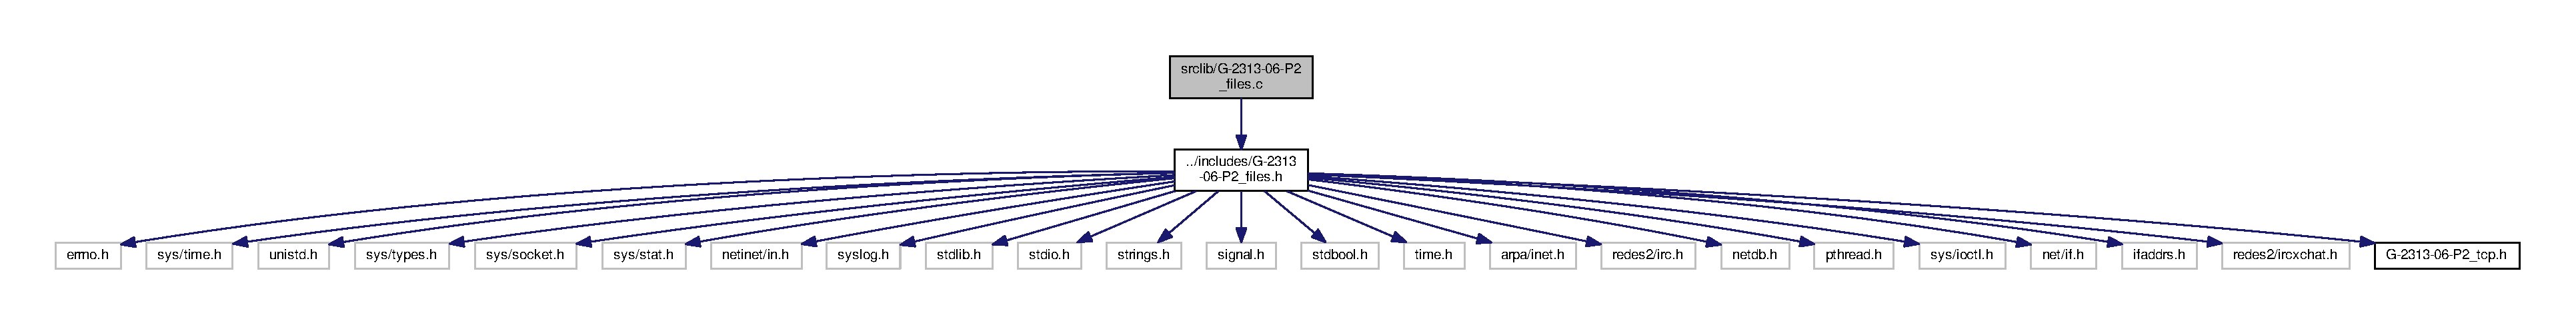
\includegraphics[width=350pt]{G-2313-06-P2__files_8c__incl}
\end{center}
\end{figure}
\subsection*{Funciones}
\begin{DoxyCompactItemize}
\item 
void $\ast$ \hyperlink{G-2313-06-P2__files_8c_ad00af19306b45db3947f1b89ae4b5def}{server\+\_\+especial\+\_\+enviar\+\_\+ficheros} (void $\ast$vrecv)
\item 
void $\ast$ \hyperlink{G-2313-06-P2__files_8c_a6796f20636727f52161d02748cb2b17e}{server\+\_\+especial\+\_\+recibir\+\_\+ficheros} (void $\ast$vmsg)
\end{DoxyCompactItemize}
\subsection*{Variables}
\begin{DoxyCompactItemize}
\item 
int \hyperlink{G-2313-06-P2__files_8c_adeadf7cb6916a10c7142ce7d265ab32a}{socket\+\_\+desc}
\item 
char $\ast$ \hyperlink{G-2313-06-P2__files_8c_ab93a317ee9a27c82844c9128a76b136a}{nick\+\_\+cliente}
\end{DoxyCompactItemize}


\subsection{Documentación de las funciones}
\index{G-\/2313-\/06-\/\+P2\+\_\+files.\+c@{G-\/2313-\/06-\/\+P2\+\_\+files.\+c}!server\+\_\+especial\+\_\+enviar\+\_\+ficheros@{server\+\_\+especial\+\_\+enviar\+\_\+ficheros}}
\index{server\+\_\+especial\+\_\+enviar\+\_\+ficheros@{server\+\_\+especial\+\_\+enviar\+\_\+ficheros}!G-\/2313-\/06-\/\+P2\+\_\+files.\+c@{G-\/2313-\/06-\/\+P2\+\_\+files.\+c}}
\subsubsection[{\texorpdfstring{server\+\_\+especial\+\_\+enviar\+\_\+ficheros(void $\ast$vrecv)}{server_especial_enviar_ficheros(void *vrecv)}}]{\setlength{\rightskip}{0pt plus 5cm}void$\ast$ server\+\_\+especial\+\_\+enviar\+\_\+ficheros (
\begin{DoxyParamCaption}
\item[{void $\ast$}]{vrecv}
\end{DoxyParamCaption}
)}\hypertarget{G-2313-06-P2__files_8c_ad00af19306b45db3947f1b89ae4b5def}{}\label{G-2313-06-P2__files_8c_ad00af19306b45db3947f1b89ae4b5def}


Definición en la línea 6 del archivo G-\/2313-\/06-\/\+P2\+\_\+files.\+c.

\index{G-\/2313-\/06-\/\+P2\+\_\+files.\+c@{G-\/2313-\/06-\/\+P2\+\_\+files.\+c}!server\+\_\+especial\+\_\+recibir\+\_\+ficheros@{server\+\_\+especial\+\_\+recibir\+\_\+ficheros}}
\index{server\+\_\+especial\+\_\+recibir\+\_\+ficheros@{server\+\_\+especial\+\_\+recibir\+\_\+ficheros}!G-\/2313-\/06-\/\+P2\+\_\+files.\+c@{G-\/2313-\/06-\/\+P2\+\_\+files.\+c}}
\subsubsection[{\texorpdfstring{server\+\_\+especial\+\_\+recibir\+\_\+ficheros(void $\ast$vmsg)}{server_especial_recibir_ficheros(void *vmsg)}}]{\setlength{\rightskip}{0pt plus 5cm}void$\ast$ server\+\_\+especial\+\_\+recibir\+\_\+ficheros (
\begin{DoxyParamCaption}
\item[{void $\ast$}]{vmsg}
\end{DoxyParamCaption}
)}\hypertarget{G-2313-06-P2__files_8c_a6796f20636727f52161d02748cb2b17e}{}\label{G-2313-06-P2__files_8c_a6796f20636727f52161d02748cb2b17e}


Definición en la línea 122 del archivo G-\/2313-\/06-\/\+P2\+\_\+files.\+c.



\subsection{Documentación de las variables}
\index{G-\/2313-\/06-\/\+P2\+\_\+files.\+c@{G-\/2313-\/06-\/\+P2\+\_\+files.\+c}!nick\+\_\+cliente@{nick\+\_\+cliente}}
\index{nick\+\_\+cliente@{nick\+\_\+cliente}!G-\/2313-\/06-\/\+P2\+\_\+files.\+c@{G-\/2313-\/06-\/\+P2\+\_\+files.\+c}}
\subsubsection[{\texorpdfstring{nick\+\_\+cliente}{nick_cliente}}]{\setlength{\rightskip}{0pt plus 5cm}char$\ast$ nick\+\_\+cliente}\hypertarget{G-2313-06-P2__files_8c_ab93a317ee9a27c82844c9128a76b136a}{}\label{G-2313-06-P2__files_8c_ab93a317ee9a27c82844c9128a76b136a}


Definición en la línea 5 del archivo G-\/2313-\/06-\/\+P2\+\_\+client.\+c.

\index{G-\/2313-\/06-\/\+P2\+\_\+files.\+c@{G-\/2313-\/06-\/\+P2\+\_\+files.\+c}!socket\+\_\+desc@{socket\+\_\+desc}}
\index{socket\+\_\+desc@{socket\+\_\+desc}!G-\/2313-\/06-\/\+P2\+\_\+files.\+c@{G-\/2313-\/06-\/\+P2\+\_\+files.\+c}}
\subsubsection[{\texorpdfstring{socket\+\_\+desc}{socket_desc}}]{\setlength{\rightskip}{0pt plus 5cm}int socket\+\_\+desc}\hypertarget{G-2313-06-P2__files_8c_adeadf7cb6916a10c7142ce7d265ab32a}{}\label{G-2313-06-P2__files_8c_adeadf7cb6916a10c7142ce7d265ab32a}


Definición en la línea 4 del archivo G-\/2313-\/06-\/\+P2\+\_\+client.\+c.


\hypertarget{G-2313-06-P2__tcp_8c}{}\section{Referencia del Archivo srclib/\+G-\/2313-\/06-\/\+P2\+\_\+tcp.c}
\label{G-2313-06-P2__tcp_8c}\index{srclib/\+G-\/2313-\/06-\/\+P2\+\_\+tcp.\+c@{srclib/\+G-\/2313-\/06-\/\+P2\+\_\+tcp.\+c}}
{\ttfamily \#include \char`\"{}../includes/\+G-\/2313-\/06-\/\+P2\+\_\+tcp.\+h\char`\"{}}\\*
{\ttfamily \#include $<$sys/socket.\+h$>$}\\*
{\ttfamily \#include $<$string.\+h$>$}\\*
{\ttfamily \#include $<$netdb.\+h$>$}\\*
{\ttfamily \#include $<$unistd.\+h$>$}\\*
Dependencia gráfica adjunta para G-\/2313-\/06-\/\+P2\+\_\+tcp.c\+:\nopagebreak
\begin{figure}[H]
\begin{center}
\leavevmode
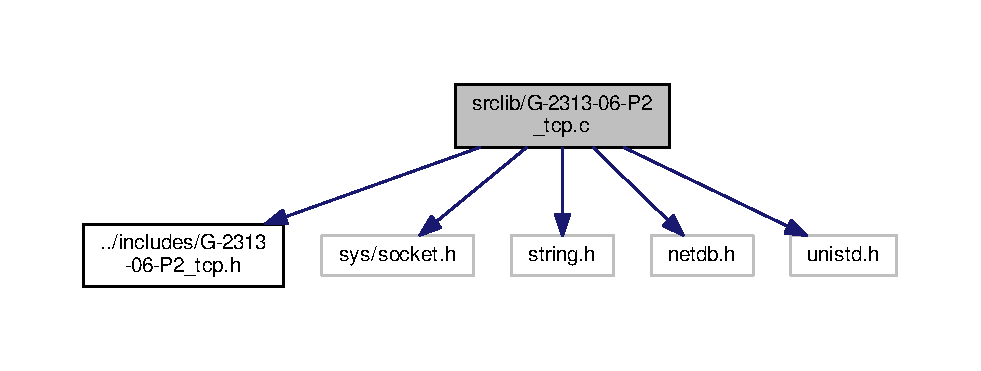
\includegraphics[width=350pt]{G-2313-06-P2__tcp_8c__incl}
\end{center}
\end{figure}
\subsection*{Funciones}
\begin{DoxyCompactItemize}
\item 
int \hyperlink{G-2313-06-P2__tcp_8c_a4e5ce422aa030ac8b3998e858b79cae2}{tcp\+\_\+connect} (char $\ast$server, int port)
\item 
int \hyperlink{G-2313-06-P2__tcp_8c_a14d727cfbcd2ce3c5f4fae5a470a84da}{tcp\+\_\+listen} (int port, int max\+\_\+conn)
\item 
int \hyperlink{G-2313-06-P2__tcp_8c_a1e2b75e457a02f23d433a6821f6902b7}{tcp\+\_\+send} (int fd, char $\ast$msg)
\item 
int \hyperlink{G-2313-06-P2__tcp_8c_af3354e60e1181adcd72f9f242063fafe}{tcp\+\_\+receive} (int fd, char $\ast$msg, int len)
\item 
int \hyperlink{G-2313-06-P2__tcp_8c_a2d1f9e76e5da3a7c1e172d1294a33611}{tcp\+\_\+disconnect} (int fd)
\end{DoxyCompactItemize}


\subsection{Documentación de las funciones}
\index{G-\/2313-\/06-\/\+P2\+\_\+tcp.\+c@{G-\/2313-\/06-\/\+P2\+\_\+tcp.\+c}!tcp\+\_\+connect@{tcp\+\_\+connect}}
\index{tcp\+\_\+connect@{tcp\+\_\+connect}!G-\/2313-\/06-\/\+P2\+\_\+tcp.\+c@{G-\/2313-\/06-\/\+P2\+\_\+tcp.\+c}}
\subsubsection[{\texorpdfstring{tcp\+\_\+connect(char $\ast$server, int port)}{tcp_connect(char *server, int port)}}]{\setlength{\rightskip}{0pt plus 5cm}int tcp\+\_\+connect (
\begin{DoxyParamCaption}
\item[{char $\ast$}]{server, }
\item[{int}]{port}
\end{DoxyParamCaption}
)}\hypertarget{G-2313-06-P2__tcp_8c_a4e5ce422aa030ac8b3998e858b79cae2}{}\label{G-2313-06-P2__tcp_8c_a4e5ce422aa030ac8b3998e858b79cae2}


Definición en la línea 7 del archivo G-\/2313-\/06-\/\+P2\+\_\+tcp.\+c.

\index{G-\/2313-\/06-\/\+P2\+\_\+tcp.\+c@{G-\/2313-\/06-\/\+P2\+\_\+tcp.\+c}!tcp\+\_\+disconnect@{tcp\+\_\+disconnect}}
\index{tcp\+\_\+disconnect@{tcp\+\_\+disconnect}!G-\/2313-\/06-\/\+P2\+\_\+tcp.\+c@{G-\/2313-\/06-\/\+P2\+\_\+tcp.\+c}}
\subsubsection[{\texorpdfstring{tcp\+\_\+disconnect(int fd)}{tcp_disconnect(int fd)}}]{\setlength{\rightskip}{0pt plus 5cm}int tcp\+\_\+disconnect (
\begin{DoxyParamCaption}
\item[{int}]{fd}
\end{DoxyParamCaption}
)}\hypertarget{G-2313-06-P2__tcp_8c_a2d1f9e76e5da3a7c1e172d1294a33611}{}\label{G-2313-06-P2__tcp_8c_a2d1f9e76e5da3a7c1e172d1294a33611}


Definición en la línea 88 del archivo G-\/2313-\/06-\/\+P2\+\_\+tcp.\+c.

\index{G-\/2313-\/06-\/\+P2\+\_\+tcp.\+c@{G-\/2313-\/06-\/\+P2\+\_\+tcp.\+c}!tcp\+\_\+listen@{tcp\+\_\+listen}}
\index{tcp\+\_\+listen@{tcp\+\_\+listen}!G-\/2313-\/06-\/\+P2\+\_\+tcp.\+c@{G-\/2313-\/06-\/\+P2\+\_\+tcp.\+c}}
\subsubsection[{\texorpdfstring{tcp\+\_\+listen(int port, int max\+\_\+conn)}{tcp_listen(int port, int max_conn)}}]{\setlength{\rightskip}{0pt plus 5cm}int tcp\+\_\+listen (
\begin{DoxyParamCaption}
\item[{int}]{port, }
\item[{int}]{max\+\_\+conn}
\end{DoxyParamCaption}
)}\hypertarget{G-2313-06-P2__tcp_8c_a14d727cfbcd2ce3c5f4fae5a470a84da}{}\label{G-2313-06-P2__tcp_8c_a14d727cfbcd2ce3c5f4fae5a470a84da}


Definición en la línea 39 del archivo G-\/2313-\/06-\/\+P2\+\_\+tcp.\+c.

\index{G-\/2313-\/06-\/\+P2\+\_\+tcp.\+c@{G-\/2313-\/06-\/\+P2\+\_\+tcp.\+c}!tcp\+\_\+receive@{tcp\+\_\+receive}}
\index{tcp\+\_\+receive@{tcp\+\_\+receive}!G-\/2313-\/06-\/\+P2\+\_\+tcp.\+c@{G-\/2313-\/06-\/\+P2\+\_\+tcp.\+c}}
\subsubsection[{\texorpdfstring{tcp\+\_\+receive(int fd, char $\ast$msg, int len)}{tcp_receive(int fd, char *msg, int len)}}]{\setlength{\rightskip}{0pt plus 5cm}int tcp\+\_\+receive (
\begin{DoxyParamCaption}
\item[{int}]{fd, }
\item[{char $\ast$}]{msg, }
\item[{int}]{len}
\end{DoxyParamCaption}
)}\hypertarget{G-2313-06-P2__tcp_8c_af3354e60e1181adcd72f9f242063fafe}{}\label{G-2313-06-P2__tcp_8c_af3354e60e1181adcd72f9f242063fafe}


Definición en la línea 81 del archivo G-\/2313-\/06-\/\+P2\+\_\+tcp.\+c.

\index{G-\/2313-\/06-\/\+P2\+\_\+tcp.\+c@{G-\/2313-\/06-\/\+P2\+\_\+tcp.\+c}!tcp\+\_\+send@{tcp\+\_\+send}}
\index{tcp\+\_\+send@{tcp\+\_\+send}!G-\/2313-\/06-\/\+P2\+\_\+tcp.\+c@{G-\/2313-\/06-\/\+P2\+\_\+tcp.\+c}}
\subsubsection[{\texorpdfstring{tcp\+\_\+send(int fd, char $\ast$msg)}{tcp_send(int fd, char *msg)}}]{\setlength{\rightskip}{0pt plus 5cm}int tcp\+\_\+send (
\begin{DoxyParamCaption}
\item[{int}]{fd, }
\item[{char $\ast$}]{msg}
\end{DoxyParamCaption}
)}\hypertarget{G-2313-06-P2__tcp_8c_a1e2b75e457a02f23d433a6821f6902b7}{}\label{G-2313-06-P2__tcp_8c_a1e2b75e457a02f23d433a6821f6902b7}


Definición en la línea 74 del archivo G-\/2313-\/06-\/\+P2\+\_\+tcp.\+c.


%--- End generated contents ---

% Index
\backmatter
\newpage
\phantomsection
\clearemptydoublepage
\addcontentsline{toc}{chapter}{Índice}
\printindex

\end{document}
